%\documentclass[11pt,a4paper]{report}
%\documentclass[11pt,a4paper,titlepage]{article}
%\documentclass[11pt,a4paper]{amsart}

\documentclass[titlepage]{article}

% 1 inch margins
\usepackage{fullpage}
\usepackage{textcomp}  % \textgreater, \textless
\usepackage{framed}
\usepackage{listings}
  \usepackage{courier}
\usepackage{amsmath}
\usepackage{verbatim}
\usepackage{graphicx}             % latex, eps
%\usepackage[pdftex]{graphicx}    % pdflatex, png, jpg, pdf
\usepackage[usenames]{color}   % dvips here screws up graphicx png version, above
\usepackage{hyperref}
%\usepackage{titletoc}

\usepackage{fancyhdr}
\pagestyle{fancy}
\fancyhf{}
\renewcommand{\headheight}{14pt}
\renewcommand{\headsep}{10pt}
\lhead{\leftmark}
\rhead{\rightmark}
\lfoot{Copyright Hilary Oliver, NIWA, 2008-2012}
\rfoot{\thepage}

\usepackage{titlepic}  % off CTAN, held locally in cylc doc dir.

\usepackage{tocloft}
% prevent double digit sub-sections crowding the toc line
\addtolength\cftsubsecnumwidth{0.5em}  % see tocloft manual

\definecolor{codeblock}{rgb}{0.95,0.95,1.0}
%\definecolor{keywords}{rgb}{1.0,0.3,0.0}
\definecolor{keywords}{rgb}{0.7,0.1,1.0}
%\definecolor{comments}{rgb}{0.0,0.7,0.8}
\definecolor{comments}{rgb}{1.0,0.4,0.0}
\definecolor{identifiers}{rgb}{0.0,0.2,0.5}
\definecolor{strings}{rgb}{0.0,0.6,0.0}
\definecolor{basic}{rgb}{0.1,0.1,0.2}
\definecolor{command}{rgb}{0.0,0.2,0.1}
\definecolor{transcr}{rgb}{0.0,0.2,0.4}
\definecolor{level1}{rgb}{1.0,0.2,1.0}
\definecolor{level2}{rgb}{0.6,0.0,0.6}
\definecolor{level3}{rgb}{0.2,0.0,0.2}

% hyperlink color:
%\definecolor{linkc}{rgb}{0,0.2,0.68}
% colored hyperlink instead of boxed
%\hypersetup{colorlinks=true, linkcolor=linkc}
\hypersetup{colorlinks=true, linkcolor=blue}

\definecolor{shadecolor}{rgb}{0.9,0.9,0.1}

\lstset{
language=,
%%xleftmargin=2em,
%%frame=single,
backgroundcolor=\color{codeblock},
basicstyle=\color{basic},
%identifierstyle=\color{identifiers},
%keywordstyle=\color{keywords},
%commentstyle=\color{comments},
%stringstyle=\color{strings},
%showstringspaces=false,
numbers=left,
%%numberstyle=\color{Gray}
}

\lstdefinelanguage{transcript}
{
showstringspaces=false,
string=[b]{"},
comment=[l][\color{comments}]{\#},
morecomment=[l][\color{command}]{\%},
}

%\lstset{
%language=bash,
%basicstyle=\color{blue}\ttfamily,
%stringstyle=\color{black},
%}

\lstdefinelanguage{suiterc}
{
showstringspaces=false,
string=[b]{"},
sensitive=true,
comment=[l]{\#},
morecomment=[s][\color{level1}]{[}{]},
morecomment=[s][\color{level2}]{[[}{]]},
morecomment=[s][\color{level3}]{[[[}{]]]},
}

\lstdefinelanguage{usage}
{
%string=[b]{"},
%sensitive=false,
%morecomment=[l]{Usage:},
%morecomment=[l]{USAGE:},
%morecomment=[l]{usage:},
%morecomment=[l]{HELP:},
%morecomment=[l]{CATEGORY:},
%morecomment=[l]{COMMANDs:},
%morecomment=[l]{Arguments:},
%morecomment=[l]{Options:},
%morecomment=[l]{arguments:},
%morecomment=[l]{command-options:},
%morecomment=[l]{COMMANDS:},
%morecomment=[l]{options:},
%%morecomment=[l]{\#},
numbers=none,
}

\lstset{
language=usage,
basicstyle=\color{basic}\ttfamily,
}

% allow \paragraph as subsubsubsection
% and \subparagraph as subsubsubsubsection
\setcounter{secnumdepth}{5}
\setcounter{tocdepth}{5}

% the follow makes \paragraph{} be followed 
% by a newline, as for section headings.
\makeatletter
\renewcommand\paragraph{%
   \@startsection{paragraph}{4}{0mm}%
      {-\baselineskip}%
      {.5\baselineskip}%
      {\normalfont\normalsize\bfseries}}
\makeatother
% and similarly for \subparagraph{} 
\makeatletter
\renewcommand\subparagraph{%
   \@startsection{subparagraph}{4}{0mm}%
      {-\baselineskip}%
      {.5\baselineskip}%
      {\normalfont\normalsize\bfseries}}
\makeatother

% define a more compact itemized list environment
\newenvironment{myitemize} {
\begin{itemize}
    \setlength{\itemsep}{1pt}
    \setlength{\parskip}{0pt}
    \setlength{\parsep}{0pt}
    \setlength{\topsep}{0pt}
    }{\end{itemize}}

% define a more compact enumerate list environment
\newenvironment{myenumerate} {
\begin{enumerate}
    \setlength{\itemsep}{1pt}
    \setlength{\parskip}{0pt}
    \setlength{\parsep}{0pt}
    \setlength{\topsep}{0pt}
    }{\end{enumerate}}

\usepackage{color}
\newcommand{\hilight}[1]{\colorbox{yellow}{#1}}

\begin{document}

 % cylc-version.txt is generated each time by doc/process
\title{The Cylc Suite Engine\\
User Guide \\
\protect \input{cylc-version.txt} \\
GNU GPL v3.0 Software License \\
Copyright (C) 2008-2013 Hilary Oliver, NIWA}

\author{Hilary Oliver}

\titlepic{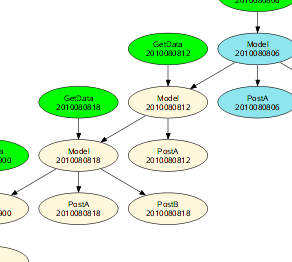
\includegraphics{graphics/png/orig/logo.png} \\

\includegraphics{graphics/png/orig/niwa-colour-small.png}}

\maketitle

%\pagebreak
%\begin{abstract}

    {\em Cylc} (``silk'') is a
    metascheduler\footnote{A metascheduler determines when dependent
    jobs are {\em ready to run} and then submits them to run by other
    means, usually a batch queue scheduler. The
    term can also refer to an aggregate view of multiple distributed
    resource managers, but that is not the topic of this document.  We
    drop the ``meta'' prefix from here on because a metascheduler is
    also a type of scheduler.} for
    cycling environmental forecasting suites containing many forecast
    models and associated processing tasks.  Cylc has a novel
    self-organising scheduling algorithm: a
    pool of task proxy objects, that each know just their own inputs and
    outputs, negotiate dependencies so that correct scheduling emerges
    naturally at run time. Cylc does not group tasks
    artificially by forecast cycle\footnote{A {\em forecast cycle}
    comprises all tasks with a common {\em cycle time} (later referred
    to here as {\em cycle point}) i.e.\ the analysis time or nominal
    start time of a forecast model, or that of the associated forecast
    model(s) for other tasks.} (each task has a private cycle time and
    is self-spawning - there is no suite-wide cycle time) and handles
    dependencies within and between cycles equally so that tasks from
    multiple cycles can run at once to the maximum possible extent. This
    matters in particular whenever the external driving data
    \footnote{Forecast suites are typically driven by real time
    observational data or timely model fields from an external
    forecasting system.} for upcoming cycles are available in advance:
    cylc suites can catch up from  delays very quickly, parallel test
    suites can be started behind the main operation to catch up quickly,
    and one can likewise achieve greater throughput in historical case
    studies; the usual sequence of distinct forecast cycles emerges
    naturally if a suite catches up to real time operation. Cylc can
    easily use existing tasks and can run suites distributed across a
    heterogenous network. Suites can be stopped and restarted in any state
    of operation, and they dynamically adapt to insertion and removal of
    tasks, and to delays or failures in particular tasks or in the
    external environment: tasks not directly affected will carry on
    cycling as normal while the problem is addressed, and then the
    affected tasks will catch up as quickly as possible. Cylc has
    comprehensive command line and graphical interfaces, including a
    dependency graph based suite control GUI. Other notable features
    include suite databases; a fast simulation mode; a structured,
    validated suite definition file format; dependency graph plotting;
    task event hooks for centralized alerting; and cryptographic suite
    security.
\end{abstract}



%\pagebreak

\tableofcontents
%\listoffigures
%\listoftables

%\pagebreak

\lstset{language=transcript}

\section{Introduction: How Cylc Works}
\label{HowCylcWorks}

\subsection{Scheduling Forecast Suites}
\label{SchedulingForecastSuites}

Environmental forecasting suites generate forecast products from a
potentially large group of interdependent scientific models and
associated data processing tasks. They are constrained by availability
of external driving data: typically one or more tasks will wait on real
time observations and/or model data from an external system, and these
will drive other downstream tasks, and so on. The dependency diagram for
a single forecast cycle point in such a system is a {\em Directed Acyclic
Graph} as shown in Figure~\ref{fig-dep-one} (in our terminology, a {\em
forecast cycle point} is comprised of all tasks with a common {\em cycle
point}, which is the nominal analysis time or start time of the forecast
models in the group). In real time operation processing will consist of
a series of distinct forecast cycle points that are each initiated, after a
gap, by arrival of the new cycle point's external driving data.

From a job scheduling perspective task execution order in such a system
must be carefully controlled in order to avoid dependency violations.
Ideally, each task should be queued for execution at the instant its
last prerequisite is satisfied; this is the best that can be done even
if queued tasks are not able to execute immediately because of resource
contention.

\subsection{EcoConnect}
\label{EcoConnect}

Cylc was developed for the EcoConnect Forecasting System at NIWA
(National Institute of Water and Atmospheric Research, New Zealand).
EcoConnect takes real time atmospheric and stream flow observations, and
operational global weather forecasts from the Met Office (UK), and uses
these to drive global sea state and regional data assimilating weather
models, which in turn drive regional sea state, storm surge, and
catchment river models, plus tide prediction, and a large number of
associated data collection, quality control, preprocessing,
post-processing, product generation, and archiving tasks.\footnote{Future
plans for EcoConnect include additional deterministic regional weather
forecasts and a statistical ensemble.} The global sea state forecast
runs once daily. The regional weather forecast runs four times daily but
it supplies surface winds and pressure to several downstream models that
run only twice daily, and precipitation accumulations to catchment river
models that run on an hourly cycle assimilating real time stream flow
observations and using the most recently available regional weather
forecast. EcoConnect runs on heterogeneous distributed hardware,
including a massively parallel supercomputer and several Linux servers.


\subsection{Dependence Between Tasks}

\subsubsection{Intra-cycle Dependence}
\label{IntracycleDependence}

Most dependence between tasks applies within a single forecast cycle
point. Figure~\ref{fig-dep-one} shows the dependency diagram for a single
forecast cycle point of a simple example suite of three forecast models
({\em a, b,} and {\em c}) and three post processing or product generation
tasks ({\em d, e} and {\em f}). A scheduler capable of handling this
must manage, within a single forecast cycle point, multiple parallel
streams of execution that branch when one task generates output for
several downstream tasks, and merge when one task takes input from several
upstream tasks.

\begin{figure}
    \begin{center}
        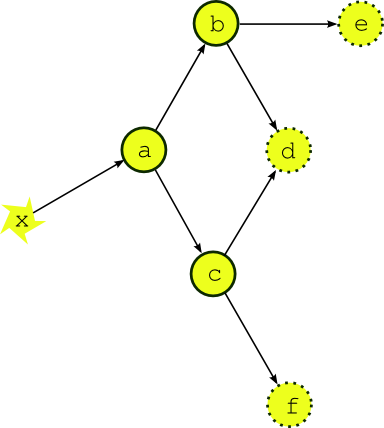
\includegraphics[width=6cm]{graphics/png/orig/dep-one-cycle.png}
    \end{center}
    \caption[A single cycle point dependency graph for a simple suite]
    {\scriptsize
    The dependency graph for a single forecast cycle point of a simple
    example suite. Tasks {\em a, b,} and {\em c} represent forecast models,
    {\em d, e} and {\em f} are post processing or product generation
    tasks, and {\em x} represents external data that the upstream
    forecast model depends on.}
    \label{fig-dep-one}
\end{figure}

\begin{figure}
    \begin{center}
        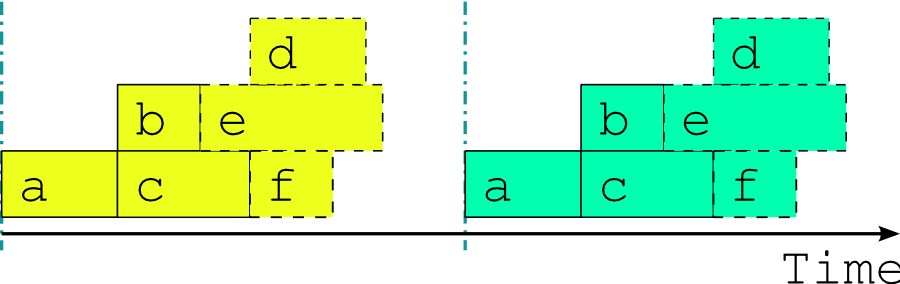
\includegraphics[width=8cm]{graphics/png/orig/timeline-one.png}
    \end{center}
    \caption[A single cycle point job schedule for real time operation]
    {\scriptsize
    The optimal job schedule for two consecutive cycle points of our
    example suite during real time operation, assuming that all tasks
    trigger off upstream tasks finishing completely. The horizontal
    extent of a task bar represents its execution time, and the vertical
    blue lines show when the external driving data becomes available.}
    \label{fig-time-one}
\end{figure}

Figure~\ref{fig-time-one} shows the optimal job schedule for two
consecutive cycle points of the example suite in real time operation, given
execution times represented by the horizontal extent of the task bars.
There is a time gap between cycle points as the suite waits on new external
driving data. Each task in the example suite happens to trigger off
upstream tasks {\em finishing}, rather than off any intermediate output
or event; this is merely a simplification that makes for clearer
diagrams.

\begin{figure}
    \begin{center}
        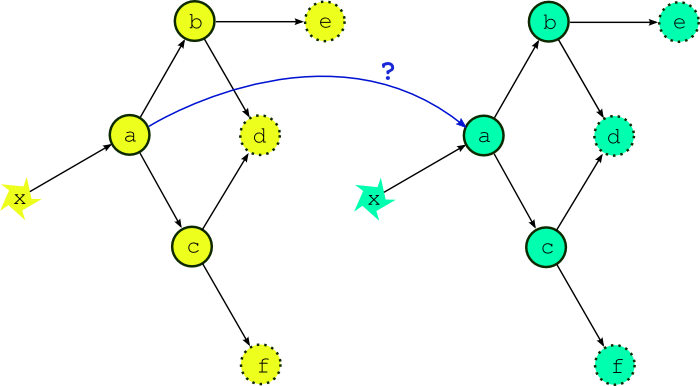
\includegraphics[width=10cm]{graphics/png/orig/dep-two-cycles-linked.png}
    \end{center}
    \caption[What if the external driving data is available early?]{\scriptsize If
    the external driving data is available in advance, can we start
    running the next cycle point early?}
    \label{fig-dep-two-linked}
\end{figure}

\begin{figure}
    \begin{center}
        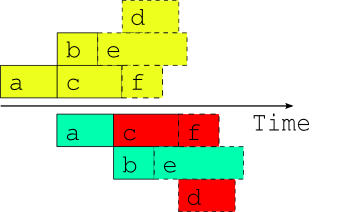
\includegraphics[width=6cm]{graphics/png/orig/timeline-one-c.png}
    \end{center}
    \caption[Attempted overlap of consecutive single-cycle-point job
    schedules]{\scriptsize A naive attempt to overlap two consecutive cycle
    points using the single-cycle-point dependency graph. The red shaded
    tasks will fail because of dependency violations (or will not be able to
    run because of upstream dependency violations).}
    \label{fig-overlap}
\end{figure}

\begin{figure}
    \begin{center}
        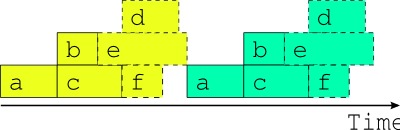
\includegraphics[width=8cm]{graphics/png/orig/timeline-one-a.png}
    \end{center}
    \caption[The only safe multi-cycle-point job schedule?]
    {\scriptsize The best that can be done {\em in general} when
    inter-cycle dependence is ignored.}
    \label{fig-job-no-overlap}
\end{figure}

Now the question arises, what happens if the external driving data for
upcoming cycle points is available in advance, as it would be after a
significant delay in operations, or when running a historical case
study?  While the forecast model {\em a} appears to depend only on the
external data {\em x} at this stage of the discussion, in fact it would
typically also depend on its own previous instance for the model {\em
background state} used in initializing the new forecast. Thus, as
alluded to in Figure~\ref{fig-dep-two-linked}, task {\em a} could in
principle start
as soon as its predecessor has finished. Figure~\ref{fig-overlap}
shows, however, that starting a whole new cycle point at this point is
dangerous - it results in dependency violations in half of the tasks in
the example suite. In fact the situation could be even worse than this
- imagine that task {\em b} in the first cycle point is delayed for some
reason {\em after} the second cycle point has been launched. Clearly we must
consider handling inter-cycle dependence explicitly or else agree not to
start the next cycle point early, as is illustrated in
Figure~\ref{fig-job-no-overlap}.

\subsubsection{Inter-Cycle Dependence}
\label{InterCyclePointDependence}

Forecast models typically depend on their own most recent previous
forecast for background state or restart files of some kind (this is
called {\em warm cycling}) but there can also be inter-cycle dependence
between different tasks. In an atmospheric forecast analysis suite, for
instance, the weather model may generate background states for observation
processing and data-assimilation tasks in the next cycle point as well as for
the next forecast model run. In real time operation inter-cycle
dependence can be ignored because it is automatically satisfied when one cycle
point finishes before the next begins. If it is not ignored it drastically
complicates the dependency graph by blurring the clean boundary between
cycle points. Figure~\ref{fig-dep-multi} illustrates the problem for our
simple example suite assuming minimal inter-cycle dependence: the warm
cycled models ($a$, $b$, and $c$) each depend on their own previous instances.

For this reason, and because we tend to see forecasting suites in terms of
their real time characteristics, other metaschedulers have ignored
inter-cycle dependence and are thus restricted to running entire cycle
points in sequence at all times. This does not affect normal real time
operation but it can be a serious impediment when advance availability of
external driving data makes it possible, in principle, to run some tasks from
upcoming cycle points before the current cycle point is finished - as was
suggested at the end of the previous section. This can occur, for instance,
after operational delays (late arrival of external data, system maintenance,
etc.) and to an even greater extent in historical case studies and parallel
test suites started behind a real time operation. It can be a serious problem
for suites that have little downtime between forecast cycle points and
therefore take many cycle points to catch up after a delay. Without taking
account of inter-cycle dependence, the best that can be done, in
general, is to reduce the gap between cycle points to zero as shown in
Figure~\ref{fig-job-no-overlap}. A limited crude overlap of the single cycle
point job schedule may be possible for specific task sets but the allowable
overlap may change if new tasks are added, and it is still dangerous: it
amounts to running different parts of a dependent system as if they were not
dependent and as such it cannot be guaranteed that some unforeseen delay in
one cycle point, after the next cycle point has begun, (e.g.\ due to resource
contention or task failures) won't result in dependency violations.

\begin{figure}
    \begin{center}
        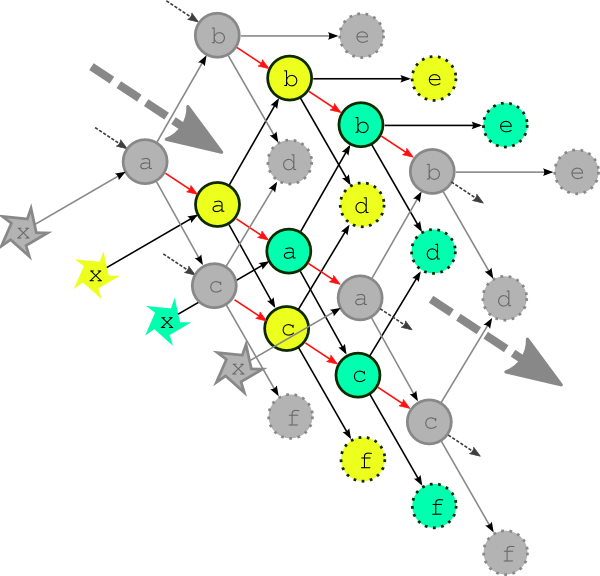
\includegraphics[width=8cm]{graphics/png/orig/dep-multi-cycle.png}
    \end{center}
    \caption[The complete multi-cycle-point dependency graph]
    {\scriptsize The complete dependency graph for the example suite, assuming
    the least possible inter-cycle dependence: the forecast models ($a$,
    $b$, and $c$) depend on their own previous instances. The dashed arrows
    show connections to previous and subsequent forecast cycle points.}
    \label{fig-dep-multi}
\end{figure}

\begin{figure}
    \begin{center}
        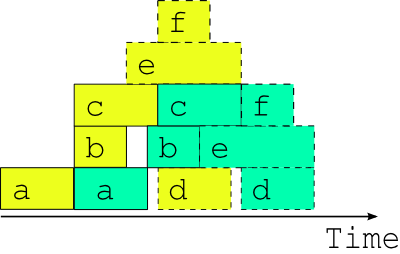
\includegraphics[width=6cm]{graphics/png/orig/timeline-two-cycles-optimal.png}
    \end{center}
    \caption[The optimal two-cycle-point job schedule]
    {\scriptsize The optimal two cycle job schedule when the next cycle's driving data is available in
    advance, possible in principle when inter-cycle dependence is
    handled explicitly.}
    \label{fig-optimal-two}
\end{figure}

Figure~\ref{fig-optimal-two} shows, in contrast to
Figure~\ref{fig-overlap}, the optimal two cycle point job schedule obtained by
respecting all inter-cycle dependence. This assumes no delays due to
resource contention or otherwise - i.e.\ every task runs
as soon as it is ready to run. The scheduler running
this suite must be able to adapt dynamically to external conditions
that impact on multi-cycle-point scheduling in the presence of
inter-cycle dependence or else, again, risk bringing the system down
with dependency violations.

\begin{figure}
    \begin{center}
        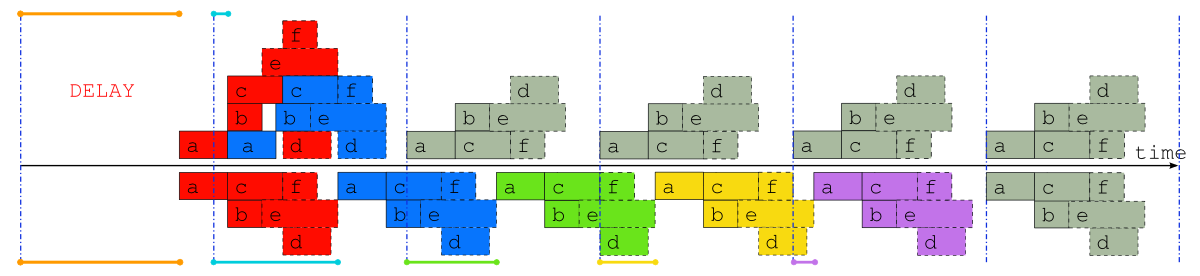
\includegraphics[width=12cm]{graphics/png/orig/timeline-three.png}
    \end{center}
    \caption[Comparison of job schedules after a delay]{\scriptsize Job
    schedules for the example suite after a delay of almost one whole
    forecast cycle point, when inter-cycle dependence is
    taken into account (above the time axis), and when it is not
    (below the time axis). The colored lines indicate the time that
    each cycle point is delayed, and normal ``caught up'' cycle points
    are shaded gray.}
    \label{fig-time-three}
\end{figure}

\begin{figure}
    \begin{center}
        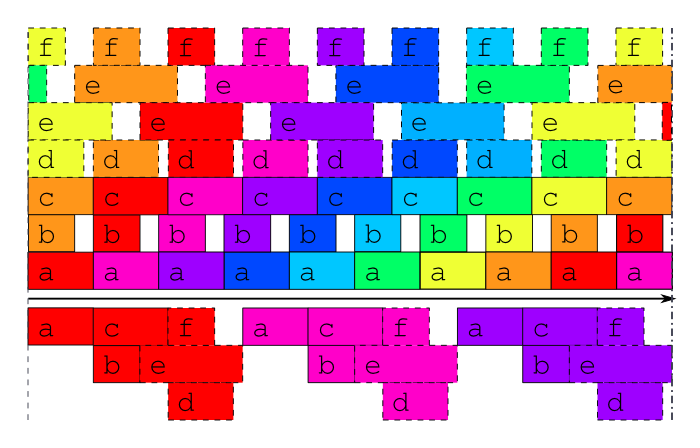
\includegraphics[width=8cm]{graphics/png/orig/timeline-two.png}
    \end{center}
    \caption[Optimal job schedule when all external data is
    available]{\scriptsize Job schedules for the example suite in case study
    mode, or after a long delay, when the external driving data are
    available many cycle points in advance. Above the time axis is the optimal
    schedule obtained when the suite is constrained only by its true
    dependencies, as in Figure \ref{fig-dep-two-linked}, and underneath
    is the best that can be done, in general, when inter-cycle
    dependence is ignored.}
    \label{fig-time-two}
\end{figure}

To further illustrate the potential benefits of proper inter-cycle
dependency handling, Figure~\ref{fig-time-three} shows an operational
delay of almost one whole cycle point in a suite with little downtime between
cycle points. Above the time axis is the optimal schedule that is possible in
principle when inter-cycle dependence is taken into account, and below
it is the only safe schedule possible {\em in general} when it is ignored.
In the former case, even the cycle point immediately after the delay is hardly
affected, and subsequent cycle points are all on time, whilst in the latter
case it takes five full cycle points to catch up to normal real time
operation.

%Note that simply overlapping the single cycle point schedules of
%Figure~\ref{fig-time-one} from the same start point would have resulted
%in dependency violation by task {\em c}.

Similarly, Figure~\ref{fig-time-two} shows example suite job schedules
for an historical case study, or when catching up after a very long
delay; i.e.\ when the external driving data are available many cycle
points in advance. Task {\em a}, which as the most upstream forecast
model is likely to be a resource intensive atmosphere or ocean model,
has no upstream dependence on co-temporal tasks and can therefore run
continuously, regardless of how much downstream processing is yet to be
completed in its own, or any previous, forecast cycle point (actually,
task {\em a} does depend on co-temporal task {\em x} which waits on the
external driving data, but that returns immediately when the data is
available in advance, so the result stands). The other forecast models
can also cycle continuously or with a short gap between, and some
post processing tasks, which have no previous-instance dependence, can
run continuously or even overlap (e.g.\ {\em e} in this case). Thus,
even for this very simple example suite, tasks from three or four
different cycle points can in principle run simultaneously at any given
time.

In fact, if our tasks are able to trigger off internal outputs of
upstream tasks (message triggers) rather than waiting on full completion,
then successive instances of the forecast models could overlap as well (because
model restart outputs are generally completed early in the forecast) for an
even more efficient job schedule.

%Finally, we note again that a good job scheduler should be able to
%dynamically adapt to delays in any part of the suite due to resource
%contention, varying run times, or anything else that will inevitably
%modify the depicted job schedules.

\subsection{The Cylc Scheduling Algorithm}
\label{TheCylcSchedulingAlgorithm}

\begin{figure}
    \begin{center}
        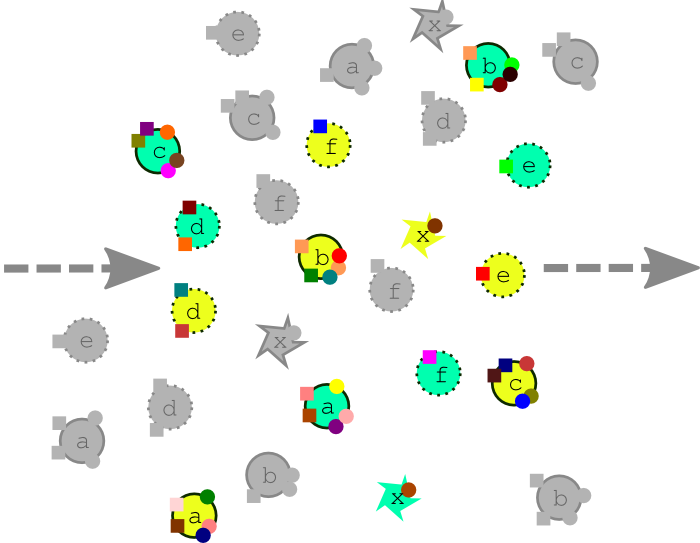
\includegraphics[width=8cm]{graphics/png/orig/task-pool.png}
    \end{center}
    \caption[The cylc task pool]{\scriptsize How cylc sees a suite, in
    contrast to the multi-cycle-point dependency graph of
    Figure~\ref{fig-dep-multi}.
    Task colors represent different cycle points, and the small squares
    and circles represent different prerequisites and outputs. A task
    can run when its prerequisites are satisfied by the outputs
    of other tasks in the pool.}
    \label{fig-task-pool}
\end{figure}

Cylc manages a pool of proxy objects that represent the real tasks in a
suite. Task proxies know how to run the real tasks that they represent,
and they receive progress messages from the tasks as they run (usually
reports of completed outputs). There is no global cycling mechanism to
advance the suite; instead individual task proxies have their own
private cycle point and spawn their own successors when the time is
right. Task proxies are self-contained - they know their own
prerequisites and outputs but are not aware of the wider suite.
Inter-cycle dependence is not treated as special, and the task pool can
be populated with tasks with many different cycle points. The task pool
is illustrated in Figure~\ref{fig-task-pool}. {\em Whenever any task
changes state due to completion of an output, every task checks to see
if its own prerequisites have been satisfied.}
%\footnote{In fact this dependency negotiation goes through a broker
%object (rather than every task literally checking every other task)
%which scales as $n$ (rather than $n^2$) where $n$ is the number of task
%proxies in the pool.}
In effect, cylc gets a pool of tasks to self-organize by negotiating
their own dependencies so that optimal scheduling, as described in the
previous section, emerges naturally at run time.

%\pagebreak
\section{Cylc Screenshots}

\begin{figure}
    \begin{center}
        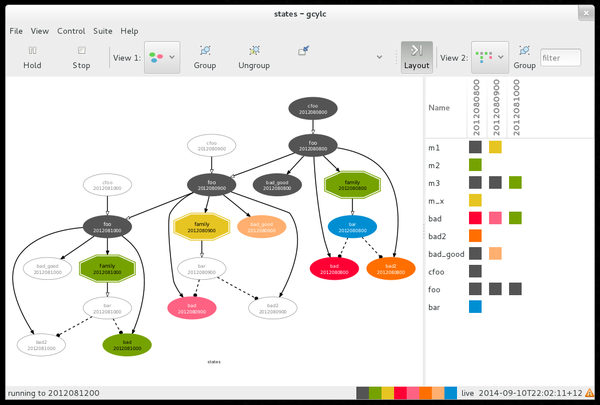
\includegraphics[width=0.8\textwidth]{graphics/png/orig/gcylc-graph-and-dot-views.png}
    \end{center}
\caption[gcylc graph and dot views]{\scriptsize gcylc graph and dot views.}
\label{fig-gcylc-1}
\end{figure}

\begin{figure}
    \begin{center}
        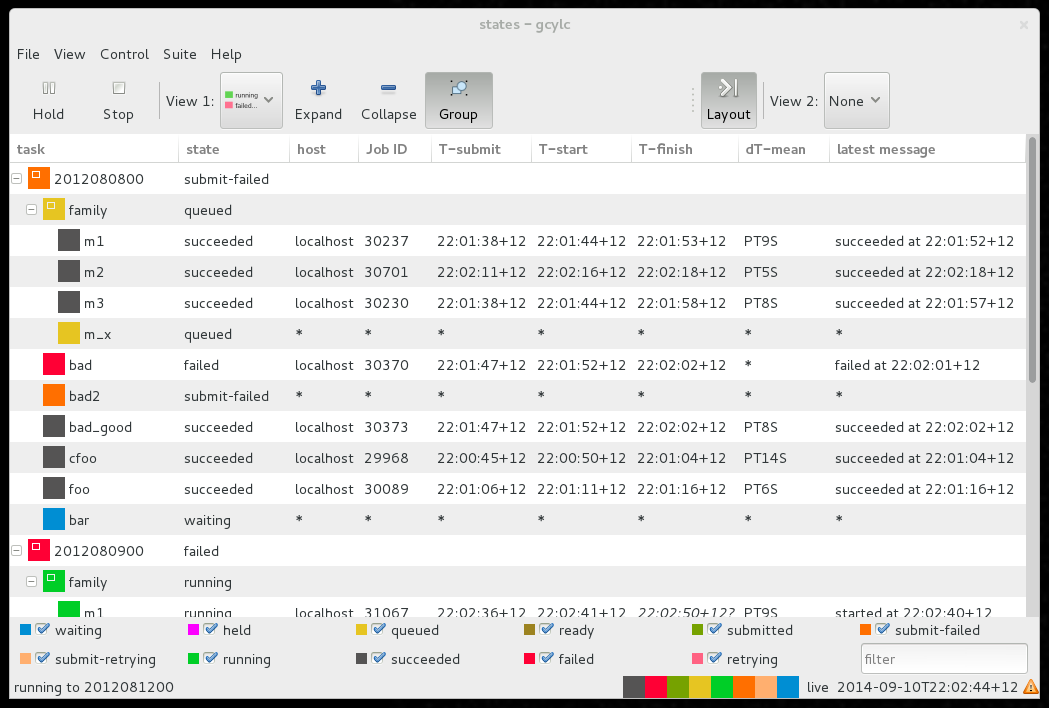
\includegraphics[width=0.8\textwidth]{graphics/png/orig/gcylc-text-view.png}
    \end{center}
\caption[gcylc text view]{\scriptsize gcylc text view.}
\label{fig-gcylc-2}
\end{figure}

\begin{figure}
    \begin{center}
        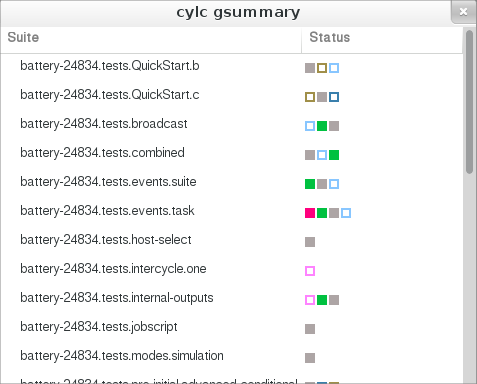
\includegraphics[width=0.5\textwidth]{graphics/png/orig/gscan.png}
    \end{center}
\caption[gscan multi-suite state summary GUI]{\scriptsize gscan multi-suite state summary GUI.}
\label{fig-gscan}
\end{figure}


\begin{figure}
    \begin{center}
        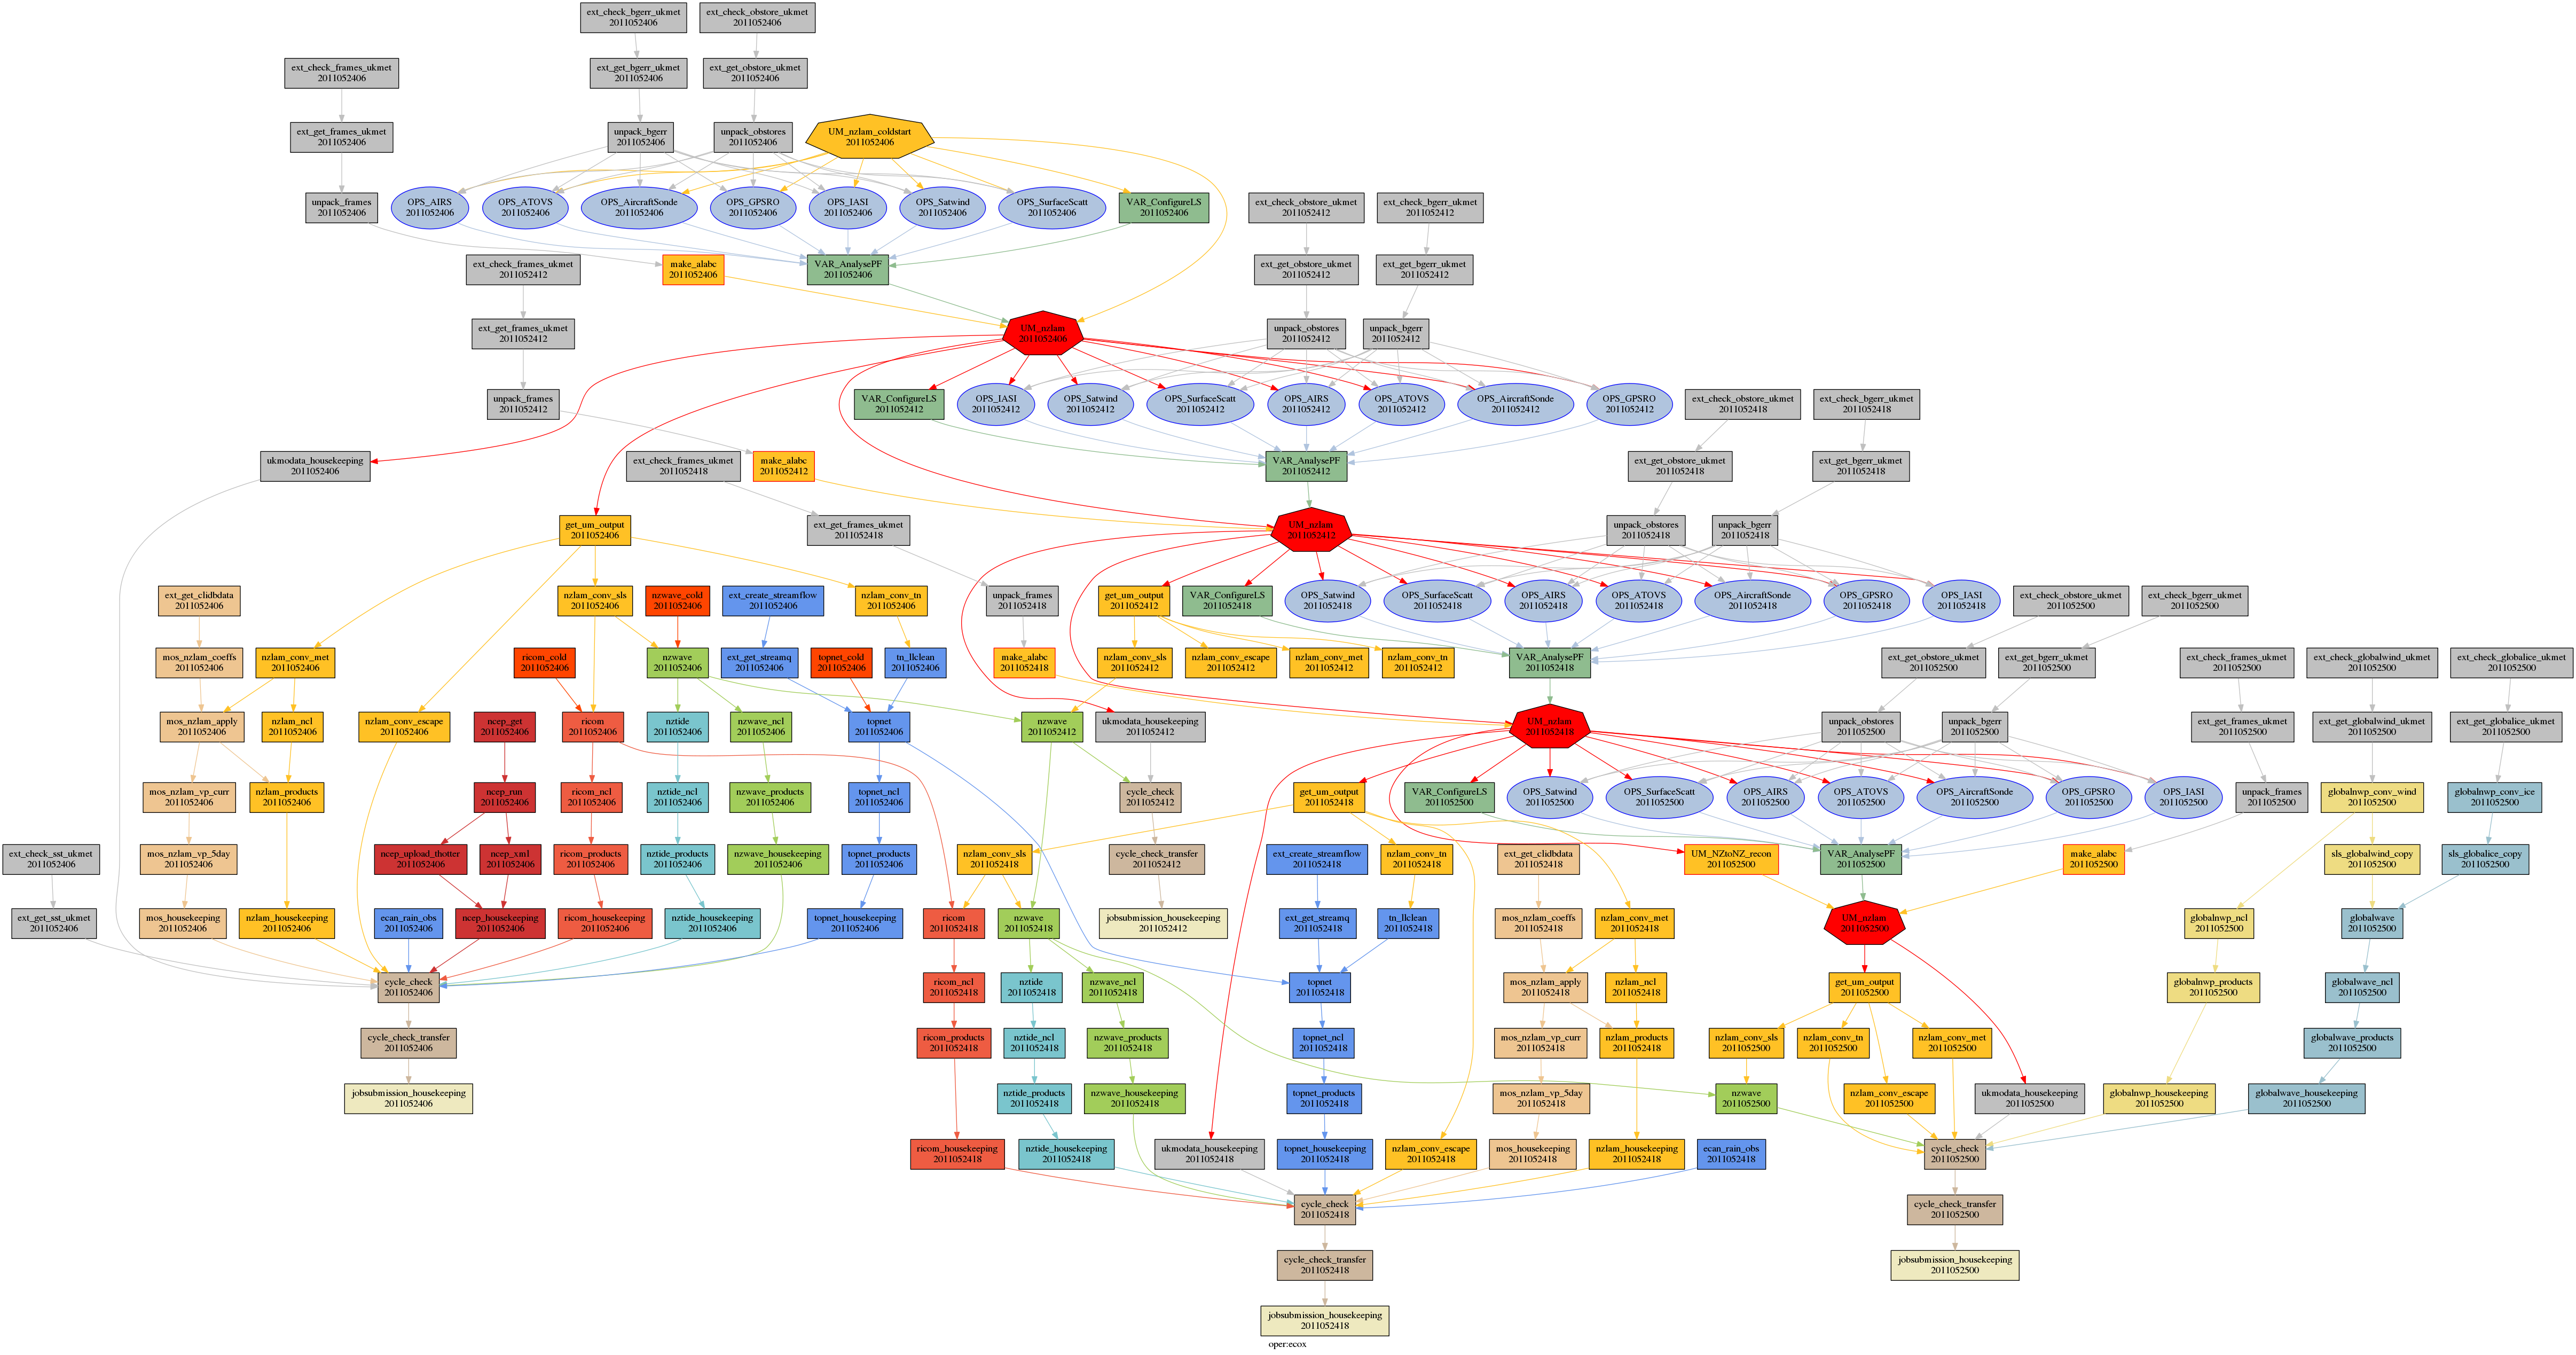
\includegraphics[width=\textwidth]{graphics/png/orig/ecox-1.png}
    \end{center}
\caption[A large-ish suite graphed by cylc]{\scriptsize A large-ish suite graphed by cylc.}
\label{fig-ecox-1}
\end{figure}

% dump floats
\clearpage

%\pagebreak

\section{Required Software}
\label{Requirements}

\begin{myitemize}
    \item {\bf Cylc}, the version associated with this document is: \input{cylc-version.txt}. % generated each time by doc/process
        \newline Cylc can be downloaded from from GitHub: \url{https://cylc.github.com/cylc}
    \item {\bf OS: A Linux or Unix variant (including, reportedly, Apple OS X).}
    \item {\bf The Python Language, version 2.6 or later, but not 3.x yet}.
        \newline \url{https://python.org}
    \item {\bf sqlite (a server-less, zero-configuration, SQL database
        engine}). The Python API to sqlite is part of the Python standard
        library. The command line interface is likely included in your Linux
        distribution already. Cylc generates an sqlite database for each suite
        as it runs, to record task events and status.
        \newline \url{http://sqlite.org}
\end{myitemize}

The following packages are technically optional as you can construct
and run cylc suites without dependency graphing and the gcylc GUI:

\begin{myitemize}
    \item {\bf PyGTK}, a Python wrapper for the GTK+ GUI toolkit,
        required for the gcylc GUI.
        PyGTK is included in most Linux Distributions.
        \newline \url{http://www.pygtk.org}
    \item {\bf Graphviz} (latest tested 2.28.0) and {\bf Pygraphviz}
        (latest tested 1.1), a graph layout engine and a Python
        interface to it.
        \newline \url{http://www.graphviz.org}
        \newline \url{http://pygraphviz.github.io/}
\end{myitemize}

If you use a binary package manager to install graphviz you may also
need a couple of {\em devel} packages for the pygraphviz build:

\begin{myitemize}
    \item python-devel
    \item graphviz-devel
\end{myitemize}

This user guide can be generated from the \LaTeX source by
running \lstinline=make= in the top level cylc directory after download.
The following \TeX packages are required (but note that the exact
packages required may be somewhat OS or distribution-dependent):

\begin{myitemize}
    \item texlive
    \item texlive-tocloft
    \item texlive-framed
    \item texlive-preprint (for fullpage.sty, formerly in tetex)
\end{myitemize}
And for HTML versions of the User Guide:

\begin{myitemize}
    \item texlive-tex4ht
    \item ImageMagick (for image scaling)
\end{myitemize}

Cylc includes a slightly modified version of cherrypy 6.0.2, a pure Python
HTTP framework that we use as a web server for communication
between server processes (cylc suites) and client programs (running tasks,
the gcylc GUI, user commands). Client communication is done via the
Python requests library if available (recommended) or via pure Python via
urllib2.
\newline \url{http://www.cherrypy.org/}
\newline \url{http://docs.python-requests.org/}

Cylc includes Jinja2 2.8, a full featured template engine for Python and its
dependency MarkupSafe 0.23, both BSD licensed.
\newline \url{http://jinja.pocoo.org/}
\newline \url{http://www.pocoo.org/projects/markupsafe/}

Finally, cylc makes heavy use of Python {\em ordered dictionary}
data structures. Significant speedup in parsing large suites can be had
by installing the
fast C-coded \lstinline=ordereddict= module by Anthon van der Neut:
\begin{myitemize}
    \item {\bf ordereddict} (latest tested 0.4.5) \newline
        \url{https://anthon.home.xs4all.nl/Python/ordereddict/}
\end{myitemize}
{\em This module is currently included with cylc} under
\lstinline=$CYLC_DIR/ext=, and is built by the top level cylc Makefile.
If you install the resulting library appropriately cylc will
automatically use it in place of a slower Python implementation of
the ordered dictionary structure.

\subsection{Known Version Compatibility Issues}

Cylc should run ``out of the box'' on recent Linux distributions.

\subsubsection{Apple Mac OSX}

It has been reported that cylc runs fine on OSX 10.6 SnowLeopard, but on
OSX 10.7 Lion there is an issue with constructing proper FQDNs (Fully
Qualified Domain Names) that requires a change to the DNS service.
Here's how to solve the problem:

\begin{myitemize}
    \item Edit \lstinline=/System/Library/LaunchDaemons/com.apple.mDNSResponder.plist= \newline
        by adding \lstinline=<string>-AlwaysAppendSearchDomains</string>= after line 16:
\begin{lstlisting}
<key>ProgramArguments</key>
  <array>
    <string>/usr/sbin/mDNSResponder</string>
    <string>-launchd</string>
        <string>-AlwaysAppendSearchDomains</string>
  </array>
\end{lstlisting}
    \item Now unload and reload the mDNSResponder service:
\begin{lstlisting}
% sudo launchctl unload -w
/System/Library/LaunchDaemons/com.apple.mDNSResponder.plist
% sudo launchctl load -w
/System/Library/LaunchDaemons/com.apple.mDNSResponder.plist
\end{lstlisting}
\end{myitemize}


\subsection{Other Software Used Internally By Cylc}

Cylc has incorporated a custom-modified version the {\em xdot} graph
viewer (\url{https://github.com/jrfonseca/xdot.py}, LGPL license).


\section{Installation}
\label{Installation}

\subsection{Install The External Dependencies}

First install graphviz, Pygraphviz, \TeX, and ImageMagick
using the package manager on your system if possible; otherwise download
the packages manually and follow their native installation documentation.
On a modern Linux system, this is very easy. For example, to install
cylc-5.1.0 on the Fedora 18 Linux distribution:

\lstset{language=transcript}
\begin{lstlisting}
shell$ yum install graphviz       # (2.28)
shell$ yum install graphviz-devel # (for pgraphviz build)
shell$ yum install python-devel   # (ditto)

# TeX packages, and ImageMagick, for generating the Cylc User Guide:
shell$ yum install texlive
shell$ yum install texlive-tex4ht
shell$ yum install texlive-tocloft
shell$ yum install texlive-framed
shell$ yum install texlive-preprint
shell$ yum install ImageMagick

# Python packages:
shell$ easy_install pygraphviz

# (sqlite 3.7.13 already installed on the system)
\end{lstlisting}

If you do not have root access on your intended cylc host machine and
cannot get a sysadmin to do this at system level, see~\ref{LocalInstall} for
tips on installing everything to a local user account.

Now check that everything other than the \LaTeX packages is
installed properly:
\lstset{language=transcript}
\begin{lstlisting}
shell$ cylc check-software
Checking for Python >= 2.6 ... found 2.7.3 ... ok
Checking for non-Python packages:
 + Graphviz ... ok
 + sqlite ... ok
Checking for Python packages:
 + pygraphviz ... ok
 + pygtk ... ok
\end{lstlisting}
If this command reports any errors then the packages concerned are not
installed, not in the system Python search path, or (for a local
install) not present in your \lstinline=$PYTHONPATH= variable.

\subsection{Install Cylc}
\label{InstallCylc}

Cylc installs into a normal user account, as an unpacked release tarball
or a git repository clone. See the \lstinline=INSTALL= file in the source
tree for instructions (also listed in~\ref{INSTALL}).

\subsubsection{Create A Site Config File}

Site and user global config files define some important parameters that affect
all suites, some of which may need to be customized for your site.
See~\ref{SiteAndUserConfiguration} for how to generate an initial site file and
where to install it. All legal site and user global config items are defined
in~\ref{SiteRCReference}.

\subsubsection{Configure Site Environment on Job Hosts}

If your users submit task jobs to hosts other than the hosts they use to run
their suites, you should ensure that the job hosts have the correct environment
for running cylc. A cylc suite generates task job scripts that normally invoke
\lstinline=bash=. The job will attempt to source the first of these files it
finds to set up its environment:

\begin{myitemize}
\item \lstinline=${HOME}/.cylc/job-init-env.sh=
\item \lstinline=${CYLC_DIR}/conf/job-init-env.sh=
\item \lstinline=${CYLC_DIR}/conf/job-init-env-default.sh=
\end{myitemize}

The \lstinline=${CYLC_DIR}/conf/job-init-env-default.sh= file is provided in
the cylc distribution, and will attempt to source \lstinline=/etc/profile= and
\lstinline=${HOME}/.profile=. If this behaviour is not desirable, you should
override it by adding a \lstinline=${CYLC_DIR}/conf/job-init-env.sh= file and
populate it with the appropriate contents.

\subsection{Automated Tests}
\label{RTAST}

The cylc test battery is primarily intended for developers to check that
changes to the source code don't break existing functionality. Note that
some test failures can be expected to result from suites timing out,
even if nothing is wrong, if you run too many tests in parallel. See
\lstinline=cylc test-battery --help=.

\subsection{Local User Installation}
\label{LocalInstall}

It is possible to install cylc and all of its software prerequisites
under your own user account. Cylc itself is already designed to be
installed into a normal user account, just follow the instructions above
in~\ref{InstallCylc}. For the other packages, depending on the
installation method used for each, it is just a matter of learning
how to change the default install path prefix from, for example,
\lstinline=/usr/local= to \lstinline=$HOME/installed/usr/local= and
then ensuring that the resulting local package paths are set properly
in your \lstinline=PYTHONPATH= environment variable.

\subsubsection{Some Guidelines}

\lstset{language=transcript}

\begin{myitemize}
\item For \lstinline=python setup.py install= installation:
\begin{lstlisting}
shell$ python setup.py install --prefix=/my/local/install/path
\end{lstlisting}
\item For building graphviz from source:
\begin{lstlisting}
shell$ ./configure --prefix=/my/local/install/path --with-qt=no
shell$ make
shell$ make install
\end{lstlisting}
The graphviz build reportedly may fail on systems that do not have QT
installed, hence the \lstinline@./configure --with-qt=no@ option above.
The graphviz lib and include locations are required when installing
Pygraphviz.
\item The pygraphviz \lstinline=setup.py= file may need to be edited
to point at your local graphviz library and include directories:
\begin{lstlisting}
# setup.py lines 31 and 32
library_path='/path/to/local/graphviz/lib'
include_path='/path/to/local/graphviz/include'
\end{lstlisting}
\item Note that when using \lstinline=python setup.py= or
\lstinline=easy_install= the local install location may need to exist
and it may be need to be present in \lstinline=PYTHONPATH= {\em before}
you initiate the install process.
\end{myitemize}

Finally, check that everything (other than \LaTeX for document
processing) is installed:

\lstset{language=transcript}
\begin{lstlisting}
shell$ cylc check-software
Checking for Python >= 2.6 ... found 2.7.3 ... ok
Checking for non-Python packages:
 + Graphviz ... ok
 + sqlite ... ok
Checking for Python packages:
 + pygraphviz ... ok
 + pygtk ... ok
\end{lstlisting}
If this command reports any errors then the packages concerned are not
installed, not in the system Python search path, or (for a local
install) not present in your \lstinline=$PYTHONPATH= variable.

\subsection{Upgrading To New Cylc Versions}

Upgrading is just a matter of unpacking the new cylc release. Successive
cylc releases can be installed in parallel as suggested in the
\lstinline=INSTALL= file (\ref{INSTALL}).

\section{{\em Cycling} And {\em Cycle Points} In Cylc}

There are several reasons why an atmospheric model (say) may need to be cycled:
\begin{myitemize}
    \item In real time forecasting it may need to wait on new real time data
        before each run.
    \item Job run length limits on compute hosts may require long jobs
        to be split into multiple shorter jobs. (This also makes
        incremental post-processing easier.)
\end{myitemize}
This section defines the terminology associated with cycling, and describes the
two ways to make a cylc workflow that cycles a model and associated jobs.

\subsection{Cycle Points}

In cylc terminology, a {\em cycle point} is a particular
date-time (or integer) point in a sequence. If a task has an hourly date-time
cycle that starts at 2014-01-01T00 and ends at 2014-01-02T00, the first cycle
point will be 2014-01-01T01, the second will be 2014-01-01T02, and so on.

You may be accustomed to the idea that a forecasting suite has a global (in the
suite-wide, not geographic, sense) cycle point that only advances when all
tasks in the current cycle point have finished (or even when a particular wall
clock time is reached, in real time operation). As explained in the
Introduction, that is not how cylc works. Rather, each task has a private cycle
point and can advance independently. The workflow is constrained only by the
dependencies of individual tasks, which may cross over to other cycle points.
It may still be convenient at times, however, to refer to the ``current cycle
point'', the ``previous cycle point'', or the ``next cycle point'' and so
forth, with reference to a particular task, or in the sense of all tasks that
``belong to'' a particular cycle point. But keep in mind that the members of
these groups may not be present simultaneously in the running suite - different
tasks may pass through the ``current cycle point'' at different times as the
suite evolves.

\subsection{Ways Of Cycling}
\label{Ways Of Cycling}

\subsubsection{Iterative Cycling}

Cylc's classic cycling mode, as described in the Introduction, can be termed
{\em iterative cycling.} The scheduler continually extends the workflow to
future cycle points as the suite runs, and each instance of a repeated job is
represented by the same logical task with a different cycle point.  For
example, a program \lstinline=model.exe= could be executed by a task
\lstinline@model@ that runs repeatedly for a series of cycle points
\lstinline=2016-01-01, 2016-01-02, 2016-01-03, ...=

This is the most powerful and flexible way of running cycling jobs in cylc, and
it is really the only way to run large operational suites that need to continue
indefinitely. The cycling is configured with general standards-based (ISO 8601)
{\em recurrence expressions} for any date-time sequence. Multiple cycling
sequences can be used at once. See Section~\ref{ConfiguringScheduling}.

\subsubsection{Parameterized Cycling}

{\em Parameterized cycling} is alternative cycling mode for workflows that are
{\em finite in extent and not too large}. Parameter expansion (or Jinja2 loops)
can be used to generate the entire workflow from start to finish, at start-up.
Once this is done, there is no sequence of cycle points in the sense defined
above, and every single instance of a repeated job is represented by a
different logical task with a different task name.  Functionally this is
entirely equivalent to defining every task instance separately in the suite
definition; parameter expansion is just a very efficient way to do that.
For example, a program \lstinline=model.exe= could be executed by each
of a series of tasks called
\lstinline=model-run0, model-run1, model-run2, ...=, where the integer
parameter values in the task names can be multiplied by an interval
(e.g.\ \lstinline=P1D= for one day) to get to the correct ``cycle point'' for
the job.

This is generally not as flexible or powerful as iterative cycling, and it has
several significant disadvantages: it is necessarily bounded (i.e.\ it can't go
on indefinitely), the difficult date-time arithmetic is not done automatically,
and at run time the full extent of the workflow (every single task instance
from start to finish) is visible at all times.  However, for smaller suites of
relatively short duration, it may be useful.  See Section~\ref{Parameterized
Cycling}.

\subsubsection{Mixed Cycling}

The two cycling approaches can be combined within a single suite.  In a daily
iterative cycling suite, for instance, long daily model runs could be split
into multiple shorter steps or chunks by parameterized cycling. (However, you
should first consider simply using a shorter iterative cycle).

\section{Global (Site, User) Configuration Files}
\label{SiteAndUserConfiguration}

Cylc site and user global configuration files contain settings that affect all
suites. Some of these, such as the range of network ports used by cylc,
should be set at site level,
\lstset{language=transcript}
\begin{lstlisting}
# cylc site global config file
/path/to/cylc/conf/global.rc
# Deprecated path to cylc site global config file
/path/to/cylc/conf/siterc/site.rc
\end{lstlisting}
Others, such as the preferred text editor for suite definitions,
can be overridden by users,
\lstset{language=transcript}
\begin{lstlisting}
# cylc user global config file
~/.cylc/global.rc
# Deprecated cylc user global config file
~/.cylc/user.rc
\end{lstlisting}

The \lstinline=cylc get-site-config= command retrieves current
global settings consisting of cylc defaults overridden by site settings,
if any, overridden by user settings, if any. To generate an
initial site or user global config file:
\lstset{language=transcript}
\begin{lstlisting}
shell$ cylc get-site-config > $HOME/.cylc/global.rc
\end{lstlisting}
Settings that do not need to be changed should be deleted or commented
out of user global config files so that they don't override future changes to
the site file.

Legal items, values, and system defaults are documented in
(\ref{SiteRCReference}).

%\pagebreak
\section{Tutorial}
\label{Tutorial}

This section provides a hands-on tutorial introduction to basic cylc
suite preparation and control. A number of features are not yet touched
on by the tutorial examples, however, so please also read the rest of
the User Guide.

\subsection{User Config File}

Some global parameters affecting cylc's behaviour are defined in a
{\em site global config file}, and can be customized per user in
{\em user global config files}. For example, to choose the text editor
invoked by cylc on suite definitions:
\lstset{language=suiterc}
\begin{lstlisting}
# $HOME/.cylc/global.rc
[editors]
    terminal = vim
    gui = gvim -f
\end{lstlisting}

\begin{myitemize}
\item For more on site and user global config files, including how to generate
one at first, see~\ref{SiteAndUserConfiguration} and~\ref{SiteRCReference}.
\end{myitemize}

\subsubsection{Configure Environment on Job Hosts}

If you submit task jobs to hosts other than the hosts you use to run your
suites, you may need to customise the environment for
running cylc. A cylc suite generates task job scripts that normally invoke
\lstinline=bash=. The job will attempt to source the first of these files it
finds to set up its environment:

\begin{myitemize}
\item \lstinline=${HOME}/.cylc/job-init-env.sh=
\item \lstinline=${CYLC_DIR}/conf/job-init-env.sh=
\item \lstinline=${CYLC_DIR}/conf/job-init-env-default.sh=
\end{myitemize}

The \lstinline=${CYLC_DIR}/conf/job-init-env-default.sh= file is provided in
the cylc distribution, and will attempt to source \lstinline=/etc/profile= and
\lstinline=${HOME}/.profile=. If this behaviour is not desirable, your site
administrator who installed cylc should have overridden it by adding a
\lstinline=${CYLC_DIR}/conf/job-init-env.sh= file and populate it with the
appropriate contents. If customisation is still required, you can add your own
\lstinline=${HOME}/.cylc/job-init-env.sh= file and populate it with the
appropriate contents.

\subsection{User Interfaces}
\label{CUI}

Cylc has command line (CLI) and graphical (GUI) user interfaces.
To access them {\em do not simply put the bin directory of the current release
the shell search path for users.} Instead, as described in the cylc INSTALL
file (\ref{INSTALL}), configure the provided multi-version wrapper script to
point to install location for any or all cylc releases. This allows existing
suites to continue running at old cylc versions if necessary.

\subsubsection{Command Line Interface (CLI)}

The command line interface is unified under a single top level
\lstinline=cylc= command that provides access to many sub-commands
and their help documentation.
\lstset{language=transcript}
\begin{lstlisting}
shell$ cylc help       # Top level command help.
shell$ cylc run --help # Example command-specific help.
\end{lstlisting}

\begin{myitemize}
    \item Command help transcripts are also printed in~\ref{CommandReference},
        and can be accessed from the \lstinline=cylc gui= Help menu.
    \item Cylc suites are {\em scriptable} because the error status returned by
        all commands can be relied on.
\end{myitemize}

\subsubsection{Graphical User Interface (GUI)}

The cylc GUI covers the same functionality as the CLI, but it has more
sophisticated suite monitoring capability. It can start and stop suites, or
connect to suites that are already running; in either case, shutting down the
GUI does not affect the suite itself.
\lstset{language=transcript}
\begin{lstlisting}
shell$ gcylc & # or:
shell$ cylc gui & # Use the File menu to switch to specific suite.
shell$ cylc gscan & # Scan GUI for multiple running suites.
\end{lstlisting}
Clicking on a suite in the scan GUI, shown in
Figure~\ref{fig-gscan}, opens a gcylc instance for it.

\subsection{Suite Definitions}

Cylc suites are defined by extended-INI format \lstinline=suite.rc=
files (the main file format extension is section nesting). These reside
in {\em suite definition directories} that may also contain a
\lstinline=bin= directory and any other suite-related files.

\begin{myitemize}
\item For more on the suite definition file format, see~\ref{SuiteDefinition}
    and~\ref{SuiteRCReference}.
\end{myitemize}

\subsection{Suite Name Registration}

Suite registration associates a name with a suite definition directory,
in a simple database. Cylc commands that parse suite definition files
can take the file path or the suite name as input; commands that
interact with running suites have to target the suite by name.
\lstset{language=transcript}
\begin{lstlisting}
# target a suite by file path:
shell$ cylc validate /path/to/my/suite/suite.rc
shell$ cylc graph /path/to/my/suite/suite.rc
# register a name for a suite:
shell$ cylc register my.suite /path/to/my/suite/
# target a suite by name:
shell$ cylc graph my.suite
shell$ cylc validate my.suite
shell$ cylc run my.suite
shell$ cylc stop my.suite
# etc.
\end{lstlisting}

\begin{myitemize}
\item For more on registering, copying, deleting, and renaming suites,
see \lstinline=cylc db --help= (see~\ref{SuiteRegistration}
and~\ref{SuiteStorageEtc}).
\end{myitemize}

\subsection{Suite Passphrases}
\label{tutPassphrases}

A suite-specific passphrase file is automatically generated in the suite
definition directory at registration time. It is loaded by the suite daemon at
start-up and used to authenticate all client connections. Clients on the suite
host account automatically load the passphrase from the suite definition
directory. The passphrase is also installed automatically in the suite run
directory on hosts for running task jobs. On other accounts that do not share
the same HOME directory with the suite host account and do not have
non-interactive SSH access to the suite host account, it is possible to install
the passphrase manually. (A client will attempt to install the passphrase
automatically via non-interactive SSH.)

Possession of a suite passphrase gives full control and full read-access to the
suite. Without it, client access is determined by the suite's public access
privilege level.

For more on connection authentication, suite passphrases, and public access,
see~\ref{ConnectionAuthentication}.

\subsection{Import The Example Suites}
\label{ImportTheExampleSuites}

Run the following command to import cylc's example suites to a chosen
directory location and register them for use under the {\em examples}
name group:
\lstset{language=transcript}
\begin{lstlisting}
shell$ cylc import-examples $TMPDIR examples
\end{lstlisting}
(first check that \lstinline=$TMPDIR= is defined in your environment, or
else use a different location). List the newly registered tutorial
suites using the \lstinline=cylc print= command:
\lstset{language=transcript}
\begin{lstlisting}
shell$ cylc db print examples.tutorial -y
examples.tutorial.oneoff.jinja2   /tmp/examples/tutorial/oneoff/jinja2
examples.tutorial.cycling.two     /tmp/examples/tutorial/cycling/two
examples.tutorial.cycling.three   /tmp/examples/tutorial/cycling/three
examples.tutorial.oneoff.remote   /tmp/examples/tutorial/oneoff/remote
# ...
\end{lstlisting}
See \lstinline=cylc db print --help= for other display options. The
tree-form display shows how hierarchical suite names can be used to
organize related suites nicely (suite names do not have to be related
to their source directory paths, although they are in this case):
\lstset{language=transcript}
\begin{lstlisting}
shell$ cylc db pr --tree -x examples.tutorial
examples
 `-tutorial
   `-cycling
   | | ...
   | |-two        Two cycling tasks with inter-cycle dependence.
   | | ...
   `-oneoff
     |-retry      A task with automatic retry on failure
     |-remote     Hello World! on a remote host
     | ...
     |-basic      The cylc Hello World! suite
     `-jobsub     Hello World! by 'at' job submission
\end{lstlisting}

\subsection{Rename The Imported Tutorial Suites}
\
Rename (re-register) the tutorial suites to make their names a bit
shorter:
\begin{lstlisting}
$ cylc rereg examples.tutorial tut
REREGISTER examples.tutorial.oneoff.jinja2 to tut.oneoff.jinja2
#...
shell$ cylc db print -x tut
tut.oneoff.external   Hello World! from an external task script
# ...
\end{lstlisting}

\subsection{Suite Validation}

Suite definitions can be validated against the \lstinline=suite.rc=
file format specification to detect many types of error without running
the suite.
\lstset{language=transcript}
\begin{lstlisting}
# pass:
shell$ cylc validate tut.oneoff.basic
Valid for cylc-6.0.0
shell$ echo $?
0
# fail:
shell$ cylc validate my.bad.suite
'Illegal item: [scheduling]special tusks'
shell$ echo $?
1
\end{lstlisting}

\subsection{Hello World in Cylc}

\hilight{ suite: \lstinline=tut.oneoff.basic= }
\vspace{3mm}

Here's the traditional {\em Hello World} program rendered as a cylc
suite:
\lstset{language=suiterc}
\lstinputlisting{../examples/tutorial/oneoff/basic/suite.rc}
\lstset{language=transcript}

Cylc suites feature a clean separation of scheduling configuration,
which determines {\em when} tasks are ready to run; and runtime
configuration, which determines {\em what} to run (and {\em where} and
{\em how} to run it) when a task is ready. In this example the
\lstinline=[scheduling]= section defines a single task called
\lstinline=hello= that triggers immediately when the suite starts
up. When the task finishes the suite shuts down. That this is a
{\em dependency graph} will be more obvious when more tasks are added.
Under the \lstinline=[runtime]= section the
\lstinline=script= item defines a simple inlined
implementation for \lstinline=hello=: it sleeps for ten seconds,
then prints \lstinline=Hello World!=, and exits. This ends up in a {\em
job script} generated by cylc to encapsulate the task (below) and,
thanks to some defaults designed to allow quick
prototyping of new suites, it is submitted to run as a background job on
the suite host. In fact cylc even provides a default task implementation
that makes the entire \lstinline=[runtime]= section technically optional:
\lstset{language=suiterc}
\lstinputlisting{../examples/tutorial/oneoff/minimal/suite.rc}
\lstset{language=transcript}
(the resulting {\em dummy task} just prints out some identifying
information and exits).

\subsection{Editing Suites}

The text editor invoked by cylc on suite definitions is determined
by cylc site and user global config files, as shown above in~\ref{CUI}.
Check that you have renamed the tutorial examples suites as described
just above and open the {\em Hello World} suite definition in your text
editor:
\lstset{language=transcript}
\begin{lstlisting}
shell$ cylc edit tut.oneoff.basic # in-terminal
shell$ cylc edit -g tut.oneoff.basic & # or GUI
\end{lstlisting}
Alternatively, start gcylc on the suite:
\lstset{language=transcript}
\begin{lstlisting}
shell$ gcylc tut.oneoff.basic &
\end{lstlisting}
and choose {\em Suite } \textrightarrow {\em Edit} from the menu.

The editor will be invoked from within the suite definition directory for easy
access to other suite files (in this case there are none). There are syntax
highlighting control files for several text editors under
\lstinline=/path/to/cylc/conf/=; see in-file comments for installation
instructions.

\subsection{Running Suites}
\label{RunningSuitesCLI}

\subsubsection{CLI}
Run \lstinline=tut.oneoff.basic= using the \lstinline=cylc run= command.
As a suite runs detailed timestamped information is written to a {\em suite
log} and progress can be followed with cylc's suite monitoring tools (below).
By default a running suite daemonizes after printing a short message so that
you can exit the terminal or even log out without killing the suite:

\lstset{language=transcript}
\begin{lstlisting}
shell$ cylc run tut.oneoff.basic
************************************************************************
*                     The Cylc Suite Engine [6.0.0]                    *
*             Copyright (C) 2008-2016 NIWA              *
*                                                                      *
* This program comes with ABSOLUTELY NO WARRANTY.  It is free software;*
* you are welcome to redistribute it under certain conditions. Details:*
*          `cylc license conditions'; `cylc license warranty'          *
************************************************************************

Suite Info:
 + Name: tut.oneoff.basic
 + PID:  29338
 + Port: 7766
 + Logs: /home/oliverh/cylc-run/tut.oneoff.basic/log/suite/{log,out,err}

To see if this suite is still running:
 * cylc scan
 * cylc ping -v tut.oneoff.basic
 * ps -fu $USER | grep 'cylc-run .* tut.oneoff.basic'

To run in non-daemon mode use --no-detach or --debug.
For more information see 'cylc --help' and the User Guide.
\end{lstlisting}

If you're quick enough (this example only takes 10-15 seconds to run) the
\lstinline=cylc scan= command will detect the running suite:
\begin{lstlisting}
shell$ cylc scan
tut.oneoff.basic oliverh oliverh-34403DL 7766

# wait 10-15 seconds ...

shell$ cylc scan
# (nothing: suite finished)
\end{lstlisting}

Using the \lstinline=--no-detach= option prevents the suite daemonizing,
but only warnings and errors, if any, are printed to the terminal.
The \lstinline=--debug= option, however, causes (among other things) task job
submission commands to to be printed stdout:

\lstset{language=transcript}
\begin{lstlisting}
shell$ cylc run --debug tut.oneoff.basic
************************************************************************
*                     The Cylc Suite Engine [6.0.0]                    *
*             Copyright (C) 2008-2016 NIWA              *
*                                                                      *
* This program comes with ABSOLUTELY NO WARRANTY.  It is free software;*
* you are welcome to redistribute it under certain conditions. Details:*
*          `cylc license conditions'; `cylc license warranty'          *
************************************************************************
cylc job-submit /home/oliverh/cylc-run/tut.oneoff.basic/log/job/1/hello/01/job
'Finished'
Suite shutting down at 2014-08-14T13:26:52+12
DONE
\end{lstlisting}
When a task is ready to run a {\em job script} is generated to run it. The
command printed just above is how cylc executes background jobs on the
suite host (this is the default), retrieves the job process ID, and directs the
output to log files in standard locations. For the log file locations that can
be seen above, in \lstinline=job/1/hello/01/= the first \lstinline=1/= is the
{\em cycle point} of the task \lstinline=hello= (for a non-cycling task
this is just the integer 1); and the final \lstinline=01/= directory is
its {\em submission number} (tasks can be made to retry on failure, manually
or automatically, in which case the submission number increments).

The suite shuts down automatically once all tasks have succeeded.

\subsubsection{GUI}

The cylc GUI can start and stop suites, or (re)connect to suites that
are already running:
\begin{lstlisting}
shell$ cylc gui tut.oneoff.basic &
\end{lstlisting}
Use the tool bar {\em Play} button, or the {\em Control}
\textrightarrow {\em Run} menu item, to run the suite again.
You may want to alter the suite definition slightly to make the task
take longer to run. Try right-clicking on the \lstinline=hello= task
to view its output logs. The relative merits of the three {\em suite
views} - dot, text, and graph - will be more apparent later when we
have more tasks. Closing the GUI does not affect the suite itself.

\subsection{Discovering Running Suites}

Suites that are currently running can be detected with command line or
GUI tools:
\begin{lstlisting}
# list currently running suites and their port numbers:
shell$ cylc scan
tut.oneoff.basic oliverh oliverh-34403DL 7766

# GUI summary view of running suites:
shell$ cylc gscan &
\end{lstlisting}

The scan GUI is shown in Figure~\ref{fig-gscan}; clicking on a suite in it
opens gcylc.

\subsection{Task Identifiers}

At run time, task instances are identified by {\em name}, which is
determined entirely by the suite definition, and a {\em cycle point} which is
usually a date-time or an integer:
\lstset{language=transcript}
\begin{lstlisting}
foo.20100808T00Z   # a task with a date-time cycle point
bar.1              # a task with an integer cycle point (could be non-cycling)
\end{lstlisting}
Non-cycling tasks usually just have the cycle point \lstinline=1=, but this
still has to be used to target the task instance with cylc commands.

\subsection{Job Submission: How Tasks Are Executed}

\hilight{ suite: \lstinline=tut.oneoff.jobsub= }
\vspace{3mm}

Task {\em job scripts} are generated by cylc to wrap the task implementation
specified in the suite definition (environment, script, etc.) in
error trapping code, messaging calls to report task progress back to the suite
daemon, and so forth. Job scripts are written to the {\em suite job log
directory} where they can be viewed alongside the job output logs. They
can be accessed at run time by right-clicking on the task in the cylc GUI, or
printed to the terminal:
\lstset{language=transcript}
\begin{lstlisting}
shell$ cylc cat-log tut.oneoff.basic hello.1
\end{lstlisting}
This command can also print the suite log (and stdout and stderr for suites
in daemon mode) and task stdout and stderr logs (see
\lstinline=cylc cat-log --help=).
A new job script can also be generated on the fly for inspection:
\lstset{language=transcript}
\begin{lstlisting}
shell$ cylc jobscript tut.oneoff.basic hello.1
\end{lstlisting}

Take a look at the job script generated for \lstinline=hello.1= during
the suite run above. The custom scripting should be clearly visible
toward the bottom of the file.

The \lstinline=hello= task in the first tutorial suite defaults to
running as a background job on the suite host. To submit it to the Unix
\lstinline=at= scheduler instead, configure its job submission settings
as in \lstinline=tut.oneoff.jobsub=:
\lstset{language=suiterc}
\begin{lstlisting}
[runtime]
    [[hello]]
        script = "sleep 10; echo Hello World!"
        [[[job]]]
            batch system = at
\end{lstlisting}
If you run the suite (first check that the {\em at daemon}
\lstinline=atd= is running on the suite host) you'll see a slightly different
job submission command printed to stdout:
\lstset{language=transcript}
\begin{lstlisting}
 cylc run --debug tut.oneoff.jobsub
************************************************************************
*        The Cylc Suite Engine [6.0.0alpha1-294-ge08560-dirty]         *
*             Copyright (C) 2008-2016 NIWA              *
*                                                                      *
* This program comes with ABSOLUTELY NO WARRANTY.  It is free software;*
* you are welcome to redistribute it under certain conditions. Details:*
*          `cylc license conditions'; `cylc license warranty'          *
************************************************************************
cylc job-submit /home/oliverh/cylc-run/tut.oneoff.jobsub/log/job/1/hello/01/job
'Finished'
Suite shutting down at 2014-08-14T14:14:43+12
DONE
\end{lstlisting}

Cylc supports a number of different job submission methods. Tasks
submitted to external batch queuing systems like \lstinline=at=,
\lstinline=PBS=, \lstinline=SLURM=, \lstinline=Moab=, or
\lstinline=LoadLeveler=, are displayed as {\em submitted} in the cylc GUI until
they actually start executing.

\begin{myitemize}
\item For more on task job scripts, see~\ref{JobScripts}.
\item For more on job submission methods, see~\ref{AvailableMethods}.
\end{myitemize}

\subsection{Locating Suite And Task Output}

If the \lstinline=--no-detach= option is not used, suite stdout and
stderr will be directed to the suite run directory along with the
time-stamped suite log file, and task job scripts and job logs
(task stdout and stderr). The default suite run directory location is
\lstinline=$HOME/cylc-run=:

\lstset{language=transcript}
\begin{lstlisting}
shell$ tree $HOME/cylc-run/tut.oneoff.basic/
|-- cylc-suite-private.db # private suite run database
|-- cylc-suite-public.db  # public suite run database
|-- cylc-suite.db         # symbolic link to public suite run database
|-- cylc-suite-env        # suite environment file
|-- share                 # suite share directory (not used in this example)
|-- work                  # task work space (sub-dirs are deleted if not used)
|    `-- 1                   # task cycle point directory (or 1)
|        `-- hello              # task work directory (deleted if not used)
|-- log                   # suite log directory
|   `-- suite                # suite daemon log directory
|   |   |-- err                 # suite daemon stderr log (daemon mode only)
|   |   |-- out                 # suite daemon stdout log (damon mode only)
|   |   `-- log                 # suite daemon event log (timestamped info)
|   `-- job                  # task job log directory
|       `-- 1                   # task cycle point directory (or 1)
|           `-- hello              # task name
|               |-- 01                # task submission number
|               |   |-- job              # task job script
|               |   `-- job-activity.log # task job activity log
|               |   |-- job.err          # task stderr log
|               |   |-- job.out          # task stdout log
|               |   `-- job.status       # task status file
|               `-- NN -> 01          # symlink to latest submission number
\end{lstlisting}
The suite run database files, suite environment file,
and task status files are used internally by cylc. Tasks execute in
private \lstinline=work/= directories that are deleted automatically
if empty when the task finishes. The suite
\lstinline=share/= directory is made available to all tasks (by
\lstinline=$CYLC_SUITE_SHARE_DIR=) as a common share space. The task submission
number increments from 1 if a task retries on failure; this is used a
sub-directory of the log tree to avoid overwriting log files from earlier
job submissions.

The top level run directory location can be changed in site and user
config files if necessary, and the suite share and work locations can be
configured separately because of the potentially larger disk space
requirement.

Task job logs can be viewed by right-clicking on tasks in the gcylc
GUI (so long as the task proxy is live in the suite), manually
accessed from the log directory (of course), or printed to the terminal
with the \lstinline=cylc cat-log= command:
\lstset{language=transcript}
\begin{lstlisting}
# suite logs:
shell$ cylc cat-log    tut.oneoff.basic           # suite event log
shell$ cylc cat-log -o tut.oneoff.basic           # suite stdout log
shell$ cylc cat-log -e tut.oneoff.basic           # suite stderr log
# task logs:
shell$ cylc cat-log    tut.oneoff.basic hello.1   # task job script
shell$ cylc cat-log -o tut.oneoff.basic hello.1   # task stdout log
shell$ cylc cat-log -e tut.oneoff.basic hello.1   # task stderr log
\end{lstlisting}
\begin{myitemize}
    \item For a web-based interface to suite and task logs (and much more),
        see {\em Rose} in~\ref{SuiteStorageEtc}.
    \item For more on environment variables supplied to tasks,
    such as \lstinline=$CYLC_SUITE_SHARE_DIR=, see~\ref{TaskExecutionEnvironment}.
\end{myitemize}

\subsection{Remote Tasks}
\label{RemoteTasks}

\hilight{ suite: \lstinline=tut.oneoff.remote= }
\vspace{3mm}

The \lstinline=hello= task in the first two tutorial suites defaults to
running on the suite host. To make it run on a remote host instead
change its runtime configuration as in \lstinline=tut.oneoff.remote=:
\lstset{language=suiterc}
\begin{lstlisting}
[runtime]
    [[hello]]
        script = "sleep 10; echo Hello World!"
        [[[remote]]]
            host = server1.niwa.co.nz
\end{lstlisting}

For remote task hosting to work several requirements must be satisfied:
\begin{myitemize}

\item Passwordless ssh must be enabled from the suite host account to
the task host account, for task job submission.

\item Your shell initialization (.profile, .bashrc, .cshrc, etc) on the remote
host must not produce any standard output as it may confuse commands such as
scp. See \url{http://www.openssh.com/faq.html#2.9} for more information.

\item Networking settings must allow communication {\em back} from
the task host to the suite host, either by network ports or ssh,
unless the last-resort one way {\em task polling} communication method
is used.

\item Cylc must be installed on the task host. Other software dependencies like
graphviz are not required there.

\item Any files needed by a remote task must be installed on the task
host. In this example there is nothing to install because the
implementation of \lstinline=hello= is inlined in the suite definition
and thus ends up entirely contained within the task job script.

\end{myitemize}

If your username is different on the task host the
\lstinline=[[[remote]]]= section also supports an
\lstinline@owner=username@ item, or your \lstinline=$HOME/.ssh/config=
file can be configured for username translation.

If you configure a task host according to the requirements above and run
the suite again in debug mode, you'll see that the job submission command
printed to suite stdout is now considerably more complicated. That's because it
has to create remote log directories, source login scripts on the remote host
to ensure cylc is visible there, send the task job script over, and submit it
to run there by the configured job submission method:

\lstset{language=transcript}
\begin{lstlisting}
shell$ cylc run --debug tut.oneoff.remote
# ...
ssh -oBatchMode=yes -oConnectTimeout=10 wrh-1.niwa.co.nz\
'CYLC_VERSION='"'"'6.1.0'"'"\
' "/opt/cylc/bin/cylc" '"'"'job-submit'"'"\
' --remote-mode "/home/oliverh/cylc-run/tut.oneoff.remote/log/job/1/hello/01/job"'
\end{lstlisting}
(Don't be intimidated by this - it is really quite straightforward and would
appear much simpler if the job log path was shorter!). Remote task job logs are
saved to the suite run directory on the task host, not on the suite host,
although they can be retrieved by right-clicking on the task in the GUI. If you
want the job logs pulled back to the suite host automatically, you can set
"retrieve job logs=True" under the "[[[remote]]]" section:

\lstset{language=suiterc}
\begin{lstlisting}
[runtime]
    [[hello]]
        script = "sleep 10; echo Hello World!"
        [[[remote]]]
            host = server1.niwa.co.nz
            retrieve job logs = True
\end{lstlisting}

The suite will attempt to \lstinline=rsync= the job logs once from the remote
host each time a task job completes. E.g. if the job file is
\lstinline=~/cylc-run/tut.oneoff.remote/log/job/1/hello/01/job=, anything under
\lstinline=~/cylc-run/tut.oneoff.remote/log/job/1/hello/01/= will be retrieved.

Some batch systems have considerable delays between the time when the job
completes and when it writes the job logs in its normal location. If this is
the case, you can configure an initial delay and retry delays for job log
retrieval by setting some delays. E.g.:

\lstset{language=suiterc}
\begin{lstlisting}
[runtime]
    [[hello]]
        script = "sleep 10; echo Hello World!"
        [[[remote]]]
            host = server1.niwa.co.nz
            retrieve job logs = True
            # Retry after 10 seconds, 1 minute and 3 minutes
            retrieve job logs retry delays = PT10S, PT1M, PT3M
\end{lstlisting}

Finally, if the disk space of the suite host is limited, you may want to set
\lstinline@[[[remote]]]retrieve job logs max size=SIZE@. The value of SIZE can
be anything that is accepted by the \lstinline@--max-size=SIZE@ option of the
\lstinline=rsync= command. E.g.:

\lstset{language=suiterc}
\begin{lstlisting}
[runtime]
    [[hello]]
        script = "sleep 10; echo Hello World!"
        [[[remote]]]
            host = server1.niwa.co.nz
            retrieve job logs = True
            # Don't get anything bigger than 10MB
            retrieve job logs max size = 10M
\end{lstlisting}

It is worth noting that cylc uses the existence of a job's \lstinline=job.out=
or \lstinline=job.err= in the local file system to indicate a successful job
log retrieval. If \lstinline=retrieve job logs max size=SIZE= is set and both
\lstinline=job.out= and \lstinline=job.err= are bigger than \lstinline=SIZE=
then cylc will consider the retrieval as failed. If retry delays are specified,
this will trigger some useless (but harmless) retries. If this occurs
regularly, you should try the following:

\begin{myitemize}
\item Reduce the verbosity of STDOUT or STDERR from the task.
\item Redirect the verbosity from STDOUT or STDERR to an alternate log file.
\item Adjust the size limit with tolerance to the expected size of STDOUT or STDERR.
\end{myitemize}

\begin{myitemize}
\item For more on remote tasks see~\ref{RunningTasksOnARemoteHost}

\item For more on task communications, see~\ref{TaskComms}.

\item For more on suite passphrases and authentication,
    see~\ref{tutPassphrases} and~\ref{ConnectionAuthentication}.
\end{myitemize}


\subsection{Task Triggering}

\hilight{ suite: \lstinline=tut.oneoff.goodbye= }
\vspace{3mm}

To make a second task called \lstinline=goodbye= trigger after
\lstinline=hello= finishes successfully, return to the original
example, \lstinline=tut.oneoff.basic=, and change the suite graph
as in \lstinline=tut.oneoff.goodbye=:
\lstset{language=suiterc}
\begin{lstlisting}
[scheduling]
    [[dependencies]]
        graph = "hello => goodbye"
\end{lstlisting}
or to trigger it at the same time as \lstinline=hello=,
\lstset{language=suiterc}
\begin{lstlisting}
[scheduling]
    [[dependencies]]
        graph = "hello & goodbye"
\end{lstlisting}
and configure the new task's behaviour under \lstinline=[runtime]=:
\lstset{language=suiterc}
\begin{lstlisting}
[runtime]
    [[goodbye]]
        script = "sleep 10; echo Goodbye World!"
\end{lstlisting}

Run \lstinline=tut.oneoff.goodbye= and check the output from the new
task:
\lstset{language=transcript}
\begin{lstlisting}
shell$ cat ~/cylc-run/tut.oneoff.goodbye/log/job/1/goodbye/01/job.out
  # or
shell$ cylc cat-log -o tut.oneoff.goodbye goodbye.1
JOB SCRIPT STARTING
cylc (scheduler - 2014-08-14T15:09:30+12): goodbye.1 started at 2014-08-14T15:09:30+12
cylc Suite and Task Identity:
  Suite Name  : tut.oneoff.goodbye
  Suite Host  : oliverh-34403dl.niwa.local
  Suite Port  : 7766
  Suite Owner : oliverh
  Task ID     : goodbye.1
  Task Host   : oliverh-34403DL
  Task Owner  : oliverh
  Task Try No.: 1

Goodbye World!
cylc (scheduler - 2014-08-14T15:09:40+12): goodbye.1 succeeded at 2014-08-14T15:09:40+12
JOB SCRIPT EXITING (TASK SUCCEEDED)
\end{lstlisting}

\subsubsection{Task Failure And Suicide Triggering}

\hilight{ suite: \lstinline=tut.oneoff.suicide= }
\vspace{3mm}

Task names in the graph string can be qualified with a state indicator
to trigger off task states other than success:
\lstset{language=suiterc}
\lstset{language=suiterc}
\begin{lstlisting}
    graph = """
 a => b        # trigger b if a succeeds
 c:submit => d # trigger d if c submits
 e:finish => f # trigger f if e succeeds or fails
 g:start  => h # trigger h if g starts executing
 i:fail   => j # trigger j if i fails
            """
\end{lstlisting}

A common use of this is to automate recovery from known modes of failure:
\lstset{language=suiterc}
\begin{lstlisting}
    graph = "goodbye:fail => really_goodbye"
\end{lstlisting}
i.e. if task \lstinline=goodbye= fails, trigger another task that
(presumably) really says goodbye.

Failure triggering generally requires use of {\em suicide triggers} as
well, to remove the recovery task if it isn't required (otherwise it
would hang about indefinitely in the waiting state):
\begin{lstlisting}
[scheduling]
    [[dependencies]]
        graph = """hello => goodbye
            goodbye:fail => really_goodbye
         goodbye => !really_goodbye # suicide"""
\end{lstlisting}
This means if \lstinline=goodbye= fails, trigger
\lstinline=really_goodbye=; and otherwise, if \lstinline=goodbye=
succeeds, remove \lstinline=really_goodbye= from the suite.

Try running \lstinline=tut.oneoff.suicide=, which also configures
the \lstinline=hello= task's runtime to make it fail, to see how this
works.
\begin{myitemize}
    \item For more on suite dependency graphs see~\ref{ConfiguringScheduling}.
    \item For more on task triggering see~\ref{TriggerTypes}.
\end{myitemize}

\subsection{Runtime Inheritance}

\hilight{ suite: \lstinline=tut.oneoff.inherit= }
\vspace{3mm}

The \lstinline=[runtime]= section is actually a {\em multiple
inheritance} hierarchy. Each subsection is a {\em namespace} that
represents a task, or if it is inherited by other namespaces, a {\em
family}. This allows common configuration to be factored out of related
tasks very efficiently.
\lstset{language=suiterc}
\lstinputlisting{../examples/tutorial/oneoff/inherit/suite.rc}
The \lstinline=[root]= namespace provides defaults for all tasks in the suite.
Here both tasks inherit \lstinline=script= from \lstinline=root=, which they
customize with different values of the environment variable
\lstinline=$GREETING=. Note that inheritance from \lstinline=root= is
implicit; from other parents an explicit \lstinline@inherit = PARENT@
is required, as shown below.

\begin{myitemize}
\item For more on runtime inheritance, see~\ref{NIORP}.
\end{myitemize}

\subsection{Triggering Families}

\hilight{ suite: \lstinline=tut.oneoff.ftrigger1= }
\vspace{3mm}

Task families defined by runtime inheritance can also be used as
shorthand in graph trigger expressions. To see this, consider two
``greeter'' tasks that trigger off another task \lstinline=foo=:
\lstset{language=suiterc}
\begin{lstlisting}
[scheduling]
    [[dependencies]]
        graph = "foo => greeter_1 & greeter_2"
\end{lstlisting}
If we put the common greeting functionality of \lstinline=greeter_1=
and \lstinline=greeter_2= into a special \lstinline=GREETERS= family,
the graph can be expressed more efficiently like this:
\lstset{language=suiterc}
\begin{lstlisting}
[scheduling]
    [[dependencies]]
        graph = "foo => GREETERS"
\end{lstlisting}
i.e.\ if \lstinline=foo= succeeds, trigger all members of
\lstinline=GREETERS= at once. Here's the full suite with runtime
hierarchy shown:
\lstset{language=suiterc}
\lstinputlisting{../examples/tutorial/oneoff/ftrigger1/suite.rc}

(Note that we recommend given ALL-CAPS names to task families to help
distinguish them from task names. However, this is just a convention).

Verbose validation shows the family member substitution done
when the suite definition is parsed:
\lstset{language=transcript}
\begin{lstlisting}
shell$ cylc val -v tut.oneoff.ftrigger1
...
Graph line substitutions occurred:
  IN: foo => GREETERS
  OUT: foo => greeter_1 & greeter_2
...
\end{lstlisting}

Experiment with the \lstinline=tut.oneoff.ftrigger1= suite to see
how this works.

\subsection{Triggering Off Families}

\hilight{ suite: \lstinline=tut.oneoff.ftrigger2= }
\vspace{3mm}

Tasks (or families) can also trigger {\em off} other families, but
in this case we need to specify what the trigger means in terms of
the upstream family members. Here's how to trigger another task
\lstinline=bar= if all members of \lstinline=GREETERS= succeed:
\lstset{language=suiterc}
\begin{lstlisting}
[scheduling]
    [[dependencies]]
        graph = """foo => GREETERS
            GREETERS:succeed-all => bar"""
\end{lstlisting}
Verbose validation in this case reports:
\lstset{language=transcript}
\begin{lstlisting}
shell$ cylc val -v tut.oneoff.ftrigger2
...
Graph line substitutions occurred:
  IN: GREETERS:succeed-all => bar
  OUT: greeter_1:succeed & greeter_2:succeed => bar
...
\end{lstlisting}
Cylc ignores family member qualifiers like \lstinline=succeed-all= on
the right side of a trigger arrow, where they don't make sense, to
allow the two graph lines above to be combined in simple cases:
\lstset{language=suiterc}
\begin{lstlisting}
[scheduling]
    [[dependencies]]
        graph = "foo => GREETERS:succeed-all => bar"
\end{lstlisting}

Any task triggering status qualified by \lstinline=-all= or
\lstinline=-any=, for the members, can be used with a family trigger.
For example, here's how to trigger \lstinline=bar= if all members
of \lstinline=GREETERS= finish (succeed or fail) and any of them them
succeed:
\lstset{language=suiterc}
\begin{lstlisting}
[scheduling]
    [[dependencies]]
        graph = """foo => GREETERS
    GREETERS:finish-all & GREETERS:succeed-any => bar"""
\end{lstlisting}
(use of \lstinline@GREETERS:succeed-any@ by itself here would trigger
\lstinline=bar= as soon as any one member of \lstinline=GREETERS=
completed successfully). Verbose validation now begins to show how
family triggers can simplify complex graphs, even for this tiny
two-member family:
\lstset{language=transcript}
\begin{lstlisting}
shell$ cylc val -v tut.oneoff.ftrigger2
...
Graph line substitutions occurred:
  IN: GREETERS:finish-all & GREETERS:succeed-any => bar
  OUT: ( greeter_1:succeed | greeter_1:fail ) & \
       ( greeter_2:succeed | greeter_2:fail ) & \
       ( greeter_1:succeed | greeter_2:succeed ) => bar
...
\end{lstlisting}

Experiment with \lstinline=tut.oneoff.ftrigger2= to see how this
works.

\begin{myitemize}
\item For more on family triggering, see~\ref{FamilyTriggers}.
\end{myitemize}

\subsection{Suite Visualization}

\lstset{language=suiterc}
You can style dependency graphs with an optional
\lstinline=[visualization]= section, as shown in
\lstinline=tut.oneoff.ftrigger2=:
\lstset{language=suiterc}
\begin{lstlisting}
[visualization]
    default node attributes = "style=filled"
    [[node attributes]]
        foo = "fillcolor=#6789ab", "color=magenta"
        GREETERS = "fillcolor=#ba9876"
        bar = "fillcolor=#89ab67"
\end{lstlisting}

To display the graph in an interactive viewer:
\lstset{language=transcript}
\begin{lstlisting}
shell$ cylc graph tut.oneoff.ftrigger2 &    # dependency graph
shell$ cylc graph -n tut.oneoff.ftrigger2 & # runtime inheritance graph
\end{lstlisting}
It should look like Figure~\ref{fig-tut-hello-multi} (with the
GREETERS family node expanded on the right).
\begin{figure}
    \begin{center}
        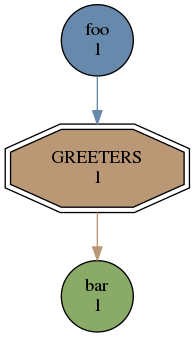
\includegraphics[height=0.3\textheight]{graphics/png/orig/tut-hello-multi-1.png}
        \hspace{20mm}
        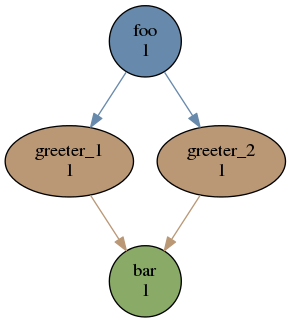
\includegraphics[height=0.3\textheight]{graphics/png/orig/tut-hello-multi-2.png}
        \hspace{20mm}
        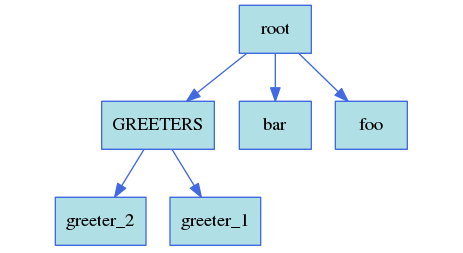
\includegraphics[height=0.3\textheight]{graphics/png/orig/tut-hello-multi-3.png}
    \end{center}
    \caption{The {\em tut.oneoff.ftrigger2} dependency and runtime inheritance graphs}
\label{fig-tut-hello-multi}
\end{figure}

Graph styling can be applied to entire families at once, and custom
``node groups'' can also be defined for non-family groups.


\subsection{External Task Scripts}

\hilight{ suite: \lstinline=tut.oneoff.external= }
\vspace{3mm}

The tasks in our examples so far have all had inlined implementation, in
the suite definition, but real tasks often need to call external
commands, scripts, or executables. To try this, let's return to the
basic Hello World suite and cut the implementation of the task
\lstinline=hello= out to a file \lstinline=hello.sh= in the suite
bin directory:
\lstset{language=bash}
\lstinputlisting{../examples/tutorial/oneoff/external/bin/hello.sh}
Make the task script executable, and change the \lstinline=hello= task
runtime section to invoke it:
\lstset{language=suiterc}
\lstinputlisting{../examples/tutorial/oneoff/external/suite.rc}

If you run the suite now the new greeting from the external task script
should appear in the \lstinline=hello= task stdout log. This works
because cylc automatically adds the suite bin directory to
\lstinline=$PATH= in the environment passed to tasks via their job
scripts. To execute scripts (etc.) located elsewhere you can
refer to the file by its full file path, or set \lstinline=$PATH=
appropriately yourself (this could be done via
\lstinline=$HOME/.profile=, which is sourced at the top of the task job
script, or in the suite definition itself).

Note the use of \lstinline=set -e= above to make the script abort on
error. This allows the error trapping code in the task job script to
automatically detect unforeseen errors.

\subsection{Cycling Tasks}

\hilight{ suite: \lstinline=tut.cycling.one= }
\vspace{3mm}

So far we've considered non-cycling tasks, which finish without spawning
a successor.

Cycling is based around iterating through date-time or integer sequences. A
cycling task may run at each cycle point in a given sequence (cycle). For
example, a sequence might be a set of date-times every 6 hours starting from a
particular date-time. A cycling task may run for each date-time item (cycle
point) in that sequence.

There may be multiple instances of this type of task running in parallel, if
the opportunity arises and their dependencies allow it. Alternatively, a
sequence can be defined with only one valid cycle point - in that case, a task
belonging to that sequence may only run once.

Open the \lstinline=tut.cycling.one= suite:
\lstset{language=suiterc}
\lstinputlisting{../examples/tutorial/cycling/one/suite.rc}
The difference between cycling and non-cycling suites is all in the
\lstinline=[scheduling]= section, so we will leave the
\lstinline=[runtime]= section alone for now (this will result in
cycling dummy tasks). Note that the graph is now defined under a new
section heading that makes each task under it have a succession of cycle points
ending in $00$ or $12$ hours, between specified initial and final cycle
points (or indefinitely if no final cycle point is given), as shown in
Figure~\ref{fig-tut-one}.

\begin{figure}
    \begin{center}
        %Q Image out of date now
        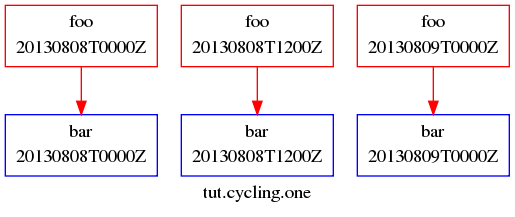
\includegraphics[width=0.5\textwidth]{graphics/png/orig/tut-one.png}
    \end{center}
    \caption{The \lstinline=tut.cycling.one= suite}
\label{fig-tut-one}
\end{figure}

\lstset{language=transcript}

If you run this suite instances of \lstinline=foo= will spawn in parallel out
to the {\em runahead limit}, and each \lstinline=bar= will trigger off the
corresponding instance of \lstinline=foo= at the same cycle point. The
runahead limit, which defaults to a few cycles but is configurable, prevents
uncontrolled spawning of cycling tasks in suites that are not constrained by
clock triggers in real time operation.

Experiment with \lstinline=tut.cycling.one= to see how cycling tasks work.

\paragraph{ISO 8601 Date-Time Syntax}

The suite above is a very simple example of a cycling date-time workflow. More
generally, cylc comprehensively supports the ISO 8601 standard for date-time
instants, intervals, and sequences. Cycling graph sections can be specified
using full ISO 8601 recurrence expressions, but these may be simplified
by assuming context information from the suite - namely initial and final cycle
points. One form of the recurrence syntax looks like
\lstinline=Rn/start-date-time/period= (\lstinline=Rn= means run
\lstinline=n= times). In the example above, if the initial cycle point
is always at 00 or 12 hours then \lstinline=[[[T00,T12]]]= could be
written as \lstinline=[[[PT12H]]]=, which is short for
\lstinline=[[[R/initial-cycle-point/PT12H/]]]= - i.e.\ run every 12 hours
indefinitely starting at the initial cycle point. It is possible to add
constraints to the suite to only allow initial cycle points at 00 or 12 hours
e.g.

\lstset{language=suiterc}
\begin{lstlisting}
[scheduling]
    initial cycle point = 20130808T00
    initial cycle point constraints = T00, T12
\end{lstlisting}
\lstset{language=transcript}

\begin{myitemize}
    %Q Runahead factor now
    \item For a comprehensive description of ISO 8601 based date-time cycling,
        see~\ref{AdvancedCycling}
    \item For more on runahead limiting in cycling suites,
        see~\ref{RunaheadLimit}.
\end{myitemize}

\subsubsection{Inter-Cycle Triggers}
\label{TutInterCyclePointTriggers}

\hilight{ suite: \lstinline=tut.cycling.two= }
\vspace{3mm}

The \lstinline=tut.cycling.two= suite adds inter-cycle dependence
to the previous example:
\begin{lstlisting}
[scheduling]
    [[dependencies]]
        # Repeat with cycle points of 00 and 12 hours every day:
        [[[T00,T12]]]
            graph = "foo[-PT12H] => foo => bar"
\end{lstlisting}
For any given cycle point in the sequence defined by the
cycling graph section heading, \lstinline=bar= triggers off
\lstinline=foo= as before, but now \lstinline=foo= triggers off its own
previous instance \lstinline=foo[-PT12H]=. Date-time offsets in
inter-cycle triggers are expressed as ISO 8601 intervals (12 hours
in this case). Figure~\ref{fig-tut-two} shows how this connects the cycling
graph sections together.
\begin{figure}
    \begin{center}
        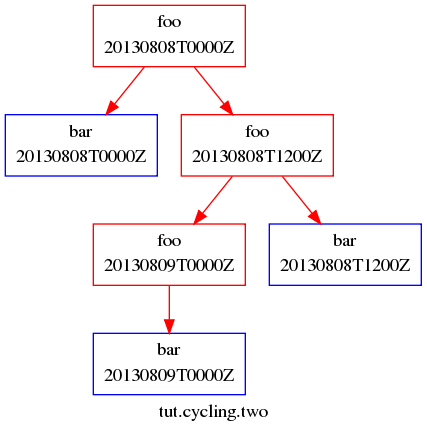
\includegraphics[width=0.5\textwidth]{graphics/png/orig/tut-two.png}
    \end{center}
    \caption{The \lstinline=tut.cycling.two= suite}
\label{fig-tut-two}
\end{figure}

Experiment with this suite to see how inter-cycle triggers work.
Note that the first instance of \lstinline=foo=, at suite start-up, will
trigger immediately in spite of its inter-cycle trigger, because cylc
ignores dependence on points earlier than the initial cycle point.
However, the presence of an inter-cycle trigger usually implies something
special has to happen at start-up. If a model depends on its own previous
instance for restart files, for example, then some special process has to
generate the initial set of restart files when there is no previous cycle point
to do it. The following section shows one way to handle this in cylc suites.

\subsubsection{Initial Non-Repeating (R1) Tasks}
\label{initial-non-repeating-r1-tasks}
\hilight{ suite: \lstinline=tut.cycling.three= }
\vspace{3mm}

Sometimes we want to be able to run a task at the initial cycle point, but
refrain from running it in subsequent cycles. We can do this by writing an
extra set of dependencies that are only valid at a single date-time cycle
point. If we choose this to be the initial cycle point, these will only apply
at the very start of the suite.

The cylc syntax for writing this single date-time cycle point occurrence is
\lstinline=R1=, which stands for
\lstinline=R1/no-specified-date-time/no-specified-period=.
This is an adaptation of part of the ISO 8601 date-time standard's recurrence
syntax (\lstinline=Rn/date-time/period=) with some special context information
supplied by cylc for the \lstinline=no-specified-*= data.

The \lstinline=1= in the \lstinline=R1= means run once. As we've specified
no date-time, Cylc will use the initial cycle point date-time by default,
which is what we want. We've also missed out specifying the period - this is
set by cylc to a zero amount of time in this case (as it never
repeats, this is not significant).

For example, in \lstinline=tut.cycling.three=:
\lstset{language=suiterc}
\begin{lstlisting}
[cylc]
    cycle point time zone = +13
[scheduling]
    initial cycle point = 20130808T00
    final cycle point = 20130812T00
    [[dependencies]]
        [[[R1]]]
            graph = "prep => foo"
        [[[T00,T12]]]
            graph = "foo[-PT12H] => foo => bar"
\end{lstlisting}
\lstset{language=transcript}
This is shown in Figure~\ref{fig-tut-three}.

Note that the time zone has been set to \lstinline=+1300= in this case,
instead of UTC (\lstinline=Z=) as before. If no time zone or UTC mode was
set, the local time zone of your machine will be used in the cycle points.


At the initial cycle point, \lstinline=foo= will depend on
\lstinline=foo[-PT12H]= and also on \lstinline=prep=:
\lstset{language=suiterc}
\begin{lstlisting}
prep.20130808T0000+13 & foo.20130807T1200+13 => foo.20130808T0000+13
\end{lstlisting}
\lstset{language=transcript}

Thereafter, it will just look like e.g.:
\lstset{language=suiterc}
\begin{lstlisting}
foo.20130808T0000+13 => foo.20130808T1200+13
\end{lstlisting}
\lstset{language=transcript}

However, in our initial cycle point example, the dependence on
\lstinline=foo.20130807T1200+13= will be ignored, because that task's cycle
point is earlier than the suite's initial cycle point and so it cannot run.
This means that the initial cycle point dependencies for \lstinline=foo=
actually look like:
\lstset{language=suiterc}
\begin{lstlisting}
prep.20130808T0000+13 => foo.20130808T0000+13
\end{lstlisting}
\lstset{language=transcript}

\begin{figure}
    \begin{center}
        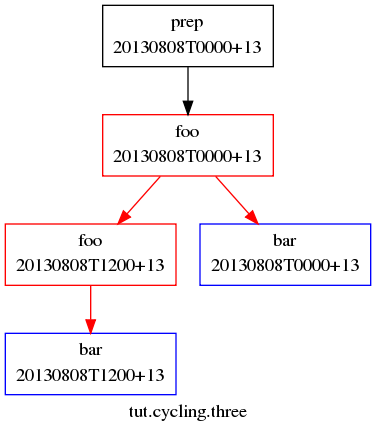
\includegraphics[width=0.5\textwidth]{graphics/png/orig/tut-three.png}
    \end{center}
    \caption{The \lstinline=tut.cycling.three= suite}
\label{fig-tut-three}
\end{figure}

\begin{myitemize}
    \item \lstinline=R1= tasks can also be used to make something special
        happen at suite shutdown, or at any single cycle point throughout the
        suite run. For a full primer on cycling syntax,
        see~\ref{AdvancedCycling}.
\end{myitemize}


\subsubsection{Integer Cycling}
\label{TutInteger}
\hilight{ suite: \lstinline=tut.cycling.integer= }
\vspace{3mm}

Cylc can do also do integer cycling for repeating workflows that are not
date-time based.

Open the \lstinline=tut.cycling.integer= suite, which is plotted in
Figure~\ref{fig-tut-int}.
\lstset{language=suiterc}
\lstinputlisting{../examples/tutorial/cycling/integer/suite.rc}

\begin{figure}
    \begin{center}
        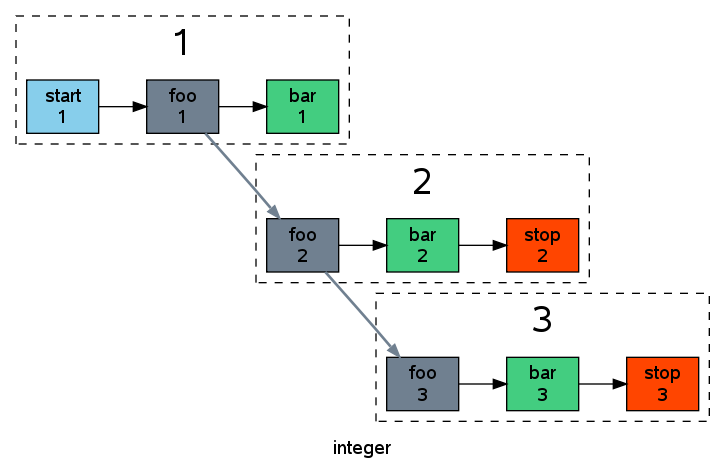
\includegraphics[width=0.65\textwidth]{graphics/png/orig/tut-cyc-int.png}
    \end{center}
    \caption{The \lstinline=tut.cycling.integer= suite}
\label{fig-tut-int}
\end{figure}

The integer cycling notation is intended to look similar to the ISO 8601
date-time notation, but it is simpler for obvious reasons. The example suite
illustrates two recurrence forms,
\lstinline=Rn/start-point/period= and
\lstinline=Rn/period/stop-point=, simplified somewhat using suite context
information (namely the initial and final cycle points). The first form is
used to run one special task called \lstinline=start= at start-up, and for the
main cycling body of the suite; and the second form to run another special task
called \lstinline=stop= in the final two cycles. The \lstinline=P= character
denotes period (interval) just like in the date-time notation.
\lstinline=R/1/P2= would generate the sequence of points \lstinline=1,3,5,...=.

\begin{myitemize}
    \item For more on integer cycling, including a more realistic usage example
        see ~\ref{IntegerCycling}.
\end{myitemize}

\subsection{Jinja2}
\hilight{ suite: \lstinline=tut.oneoff.jinja2= }
\vspace{3mm}

Cylc has built in support for the Jinja2 template processor, which
allows us to embed code in suite definitions to generate the
final result seen by cylc.

The \lstinline=tut.oneoff.jinja2= suite illustrates two common
uses of Jinja2: changing suite content or structure based on the value
of a logical switch; and iteratively generating dependencies and runtime
configuration for groups of related tasks:
\lstset{language=suiterc}
\lstinputlisting{../examples/tutorial/oneoff/jinja2/suite.rc}

To view the result of Jinja2 processing with the Jinja2 flag
\lstinline@MULTI@ set to \lstinline=False=:
\lstset{language=transcript}
\begin{lstlisting}
shell$ cylc view --jinja2 --stdout tut.oneoff.jinja2
\end{lstlisting}
\lstset{language=suiterc}
\begin{lstlisting}
title = "A Jinja2 Hello World! suite"
[scheduling]
    [[dependencies]]
        graph = "hello"
[runtime]
    [[hello]]
        script = "sleep 10; echo Hello World!"
\end{lstlisting}

And with \lstinline=MULTI= set to \lstinline=True=:
\lstset{language=transcript}
\begin{lstlisting}
shell$ cylc view --jinja2 --stdout tut.oneoff.jinja2
\end{lstlisting}
\lstset{language=suiterc}
\begin{lstlisting}
title = "A Jinja2 Hello World! suite"
[scheduling]
    [[dependencies]]
        graph = "hello => BYE"
[runtime]
    [[hello]]
        script = "sleep 10; echo Hello World!"
    [[BYE]]
        script = "sleep 10; echo Goodbye World!"
    [[ goodbye_0 ]]
        inherit = BYE
    [[ goodbye_1 ]]
        inherit = BYE
    [[ goodbye_2 ]]
        inherit = BYE
\end{lstlisting}

\subsection{Task Retry On Failure}

\hilight{ suite: \lstinline=tut.oneoff.retry= }
\vspace{3mm}

Tasks can be configured to retry a number of times if they fail.
An environment variable \lstinline=$CYLC_TASK_TRY_NUMBER= increments
from $1$ on each successive try, and is passed to the task to allow
different behaviour on the retry:
\lstset{language=suiterc}
\lstinputlisting{../examples/tutorial/oneoff/retry/suite.rc}

When a task with configured retries fails, its cylc task proxy goes
into the {\em retrying} state until the next retry delay is up, then it
resubmits. It only enters the {\em failed} state on a final definitive
failure.

Experiment with \lstinline=tut.oneoff.retry= to see how this works.

\subsection{Other Users' Suites}

If you have read access to another user's account (even on another host)
it is possible to use \lstinline=cylc monitor= to look at their suite's
progress without full shell access to their account. To do this, you
will need to copy their suite passphrase to
\lstset{language=transcript}
\begin{lstlisting}
    $HOME/.cylc/SUITE_OWNER@SUITE_HOST/SUITE_NAME/passphrase
\end{lstlisting}
(use of the host and owner names is optional here - see~\ref{passphrases})
{\em and} also retrieve the port number of the running suite from:
\begin{lstlisting}
    ~SUITE_OWNER/.cylc/ports/SUITE_NAME
\end{lstlisting}
Once you have this information, you can run
\begin{lstlisting}
shell$ cylc monitor --user=SUITE_OWNER --port=SUITE_PORT SUITE_NAME
\end{lstlisting}
to view the progress of their suite.

Other suite-connecting commands work in the same way too;
see~\ref{RemoteControl}.

\subsection{Searching A Suite}

The cylc suite search tool reports pattern matches in the suite definition
by line number, suite section, and file, even if the suite uses nested
include-files, and by file and line number for matches in suite bin
scripts:
\lstset{language=transcript}

\begin{lstlisting}
shell$ cylc search examples/admin/suite.rc OUTPUT_DIR

FILE: /home/hilary/cylc/examples/admin/suite.rc
   SECTION: [runtime]->[[root]]->[[[environment]]]
      (52):             OUTPUT_DIR = $WORKSPACE

FILE: /home/hilary/cylc/examples/admin/bin/A.sh
   (28): touch $OUTPUT_DIR/surface-winds-${CYLC_TASK_CYCLE_POINT}.nc
   (29): touch $OUTPUT_DIR/precipitation-${CYLC_TASK_CYCLE_POINT}.nc

#...
\end{lstlisting}

\subsection{Other Things To Try}

Almost every feature of cylc can be tested quickly and easily with a
simple dummy suite. You can write your own, or start from one of the
example suites in \lstinline=/path/to/cylc/examples= (see use of
\lstinline=cylc import-examples= above) - they all run ``out the box''
and can be copied and modified at will.

\begin{myitemize}

\item Change the suite runahead limit in a cycling suite.

\item Stop a suite mid-run with \lstinline=cylc stop=, and restart
it again with \lstinline=cylc restart=.

\item Hold (pause) a suite mid-run with \lstinline=cylc hold=,
    then modify the suite definition and \lstinline=cylc reload= it
    before using \lstinline=cylc release= to continue (you can also
    reload without holding).

\item Use the gcylc View menu to show the task state color key and
watch tasks in the \lstinline=task-states= example evolve
as the suite runs.

\item Manually re-run a task that has already completed or failed,
    with \lstinline=cylc trigger=.

\item Use an {\em internal queue} to prevent more than an alotted number
    of tasks from running at once even though they are ready -
   see~\ref{InternalQueues}.

\item Configure task event hooks to send an email, or shut the suite down,
    on task failure.

\end{myitemize}


\section{Suite Name Registration}
\label{SuiteRegistration}

Cylc commands target suites via names registered in a {\em suite name
database} located at \lstinline=$HOME/.cylc/REGDB/=. Suite names are
hierarchical like directory paths, allowing nested tree-like grouping,
but use the `.' character as a delimiter. This :
\begin{lstlisting}
shell$ cylc db print -t nwp
nwp
 |-oper
 | |-region1  Local Model Region1       /oper/nwp/suites/LocalModel/nested/Region1
 | `-region2  Local Model Region2       /oper/nwp/suites/LocalModel/nested/Region2
 `-test
   `-region1  Local Model TEST Region1  /home/hilary/suites/Regional/TESTS/Region1
\end{lstlisting}

Suite titles held in the name database are parsed from the suite
definition at the time of initial suite registration. If you change the
title later use \lstinline=cylc db refresh= to update the database.

Name groups are entirely virtual, they do not need to be
explicitly created before use, and they automatically disappear if all
tasks are removed from them. From the listing above, for example, to
move the suite \lstinline=nwp.oper.region2= into the
\lstinline=nwp.test= group:
\begin{lstlisting}
shell$ cylc db rereg nwp.oper.region2 nwp.test.region2
REREGISTER nwp.oper.region2 to nwp.test.region2
shell$ cylc db print -tx nwp
nwp
 |-oper
 | `-region1  Local Model Region1
 `-test
   |-region1  Local Model TEST Region1
   `-region2  Local Model Region2
\end{lstlisting}
And to move \lstinline=nwp.test.region2= into a new group \lstinline=nwp.para=:
\begin{lstlisting}
shell$ cylc db rereg nwp.test.region2 nwp.para.region2
REREGISTER nwp.test.region2 to nwp.para.region2
shell$ cylc db print -tx nwp
nwp
 |-oper
 | `-region1  Local Model Region1
 |-test
 | `-region1  Local Model TEST Region1
 `-para
   `-region2  Local Model Region2
\end{lstlisting}

Currently you cannot explicitly indicate a group name on the command
line by appending a dot character. Rather, in database operations such
as copy, reregister, or unregister, the identity of the source item
(group or suite) is inferred from the content of the database; and if
the source item is a group, so must the target be a group (or it will
be, in the case of an item that will be created by the operation). This
means that you cannot copy a single suite into a group that does not
exist yet unless you specify the entire target suite name.

\lstinline=cylc db register --help= shows a number of other examples.

\subsection{Suite Name Registration Commands}

On the command line, the  `database' (or `db') command category contains
commands to implement the aforementioned operations.

\lstset{language=usage}
\begin{lstlisting}
shell$ cylc db help
CATEGORY: db|database - Suite name registration, copying, deletion, etc.

Suite name registrations are held in a simple database $HOME/.cylc/REGDB
$ cat $HOME/.cylc/REGDB/my.suite
   title=my suite title
   path=/path/to/my/suite

HELP: cylc [db|database] COMMAND help,--help
  You can abbreviate db|database and COMMAND.
  The category db|database may be omitted.

COMMANDS:
  copy|cp ............. Copy a suite or a group of suites
  get-directory ....... Retrieve suite definition directory paths
  print ............... Print registered suites
  refresh ............. Report invalid registrations and update suite titles
  register ............ Register a suite for use
  reregister|rename ... Change the name of a suite
  unregister .......... Unregister and optionally delete suites
\end{lstlisting}

Groups of suites (at any level in the name hierarchy) can be deleted,
copied, imported, and exported; as well as individual suites. To do this,
just use suite group names as source and/or target for operations, as
appropriate. For instance, if a group \lstinline=foo.bar= contains the
suites \lstinline=foo.bar.baz= and \lstinline=foo.bar.qux=, you can copy
a single suite like this:
\lstset{language=transcript}
\begin{lstlisting}
shell$ cylc copy foo.bar.baz boo $HOME/suites
\end{lstlisting}
(resulting in a new suite \lstinline=boo=); or the group like this:
\lstset{language=transcript}
\begin{lstlisting}
shell$ cylc copy foo.bar boo $HOME/suites
\end{lstlisting}
(resulting in new suites \lstinline=boo.baz= and \lstinline=boo.qux=); or the group like this:
\lstset{language=transcript}
\begin{lstlisting}
shell$ cylc copy foo boo $HOME/suites
\end{lstlisting}
(resulting in new suites \lstinline=boo.bar.baz= and \lstinline=boo.bar.qux=).
When suites are copied, the suite definition directories are copied into
a directory tree, under the target directory, that reflects the
suite name hierarchy. \lstinline=cylc copy --help= has some explicit examples.

The same functionality is also available by right-clicking on suites
or groups in the gcylc ``Open Registered Suite'' dialog.


%\pagebreak
\section{Suite Definition}
\label{SuiteDefinition}

Cylc suites are defined in structured, validated, {\em suite.rc} files
that concisely specify the properties of, and the relationships
between, the various tasks managed by the suite. This section of the
User Guide deals with the format and content of the suite.rc file,
including task definition. Task implementation - what's required of the
real commands, scripts, or programs that do the processing that the
tasks represent - is covered in~\ref{TaskImplementation}; and
task job submission - how tasks are submitted to run - is
in~\ref{TaskJobSubmission}.

\subsection{Suite Definition Directories}
\label{SuiteDefinitionDirectories}

A cylc {\em suite definition directory} contains:
\begin{myitemize}
    \item {\bf A suite.rc file}: this is the suite definition.
        \begin{myitemize}
            \item And any include-files used in it (see below; may be
                kept in sub-directories).
        \end{myitemize}
    \item {\bf A \lstinline=bin/= sub-directory} (optional)
        \begin{myitemize}
            \item For scripts and executables that implement, or are
                used by, suite tasks.
            \item Automatically added to \lstinline=$PATH= in task
                execution environments.
            \item Alternatively, tasks can call external
                commands, scripts, or programs; or they can be scripted
                entirely within the suite.rc file.
        \end{myitemize}
    \item {\bf A \lstinline=lib/python/= sub-directory} (optional)
        \begin{myitemize}
            \item For custom job submission modules
                (see~\ref{CustomJobSubmissionMethods})
                and local Python modules imported by custom Jinja2 filters
                (see~\ref{CustomJinja2Filters}).
        \end{myitemize}
    \item {\bf Any other sub-directories and files} - documentation,
        control files, etc. (optional)
        \begin{myitemize}
            \item Holding everything in one place makes proper suite
                revision control possible.
            \item Portable access to files here, for running tasks, is
                provided through
                \lstinline=$CYLC_SUITE_DEF_PATH=
                (see~\ref{TaskExecutionEnvironment}).
            \item Ignored by cylc, but the entire suite definition
                directory tree is copied when you copy a
                suite using cylc commands.

        \end{myitemize}
\end{myitemize}
A typical example:
\lstset{language=transcript}
\begin{lstlisting}
/path/to/my/suite   # suite definition directory
    suite.rc           # THE SUITE DEFINITION FILE
    bin/               # scripts and executables used by tasks
        foo.sh
        bar.sh
        ...
    # (OPTIONAL) any other suite-related files, for example:
    inc/               # suite.rc include-files
        nwp-tasks.rc
        globals.rc
        ...
    doc/               # documentation
    control/           # control files
    ancil/             # ancillary files
    ...
\end{lstlisting}

\subsection{Suite.rc File Overview}
\label{SuiteRCFile}

Suite.rc files are an extended-INI format with section nesting.

Embedded template processor expressions may also be used in the file, to
programatically generate the final suite definition seen by
cylc. Currently the Jinja2 template processor is supported
(\url{http://jinja.pocoo.org/docs}); see~\ref{Jinja2} for examples. In the
future cylc may provide a plug-in interface to allow use of other template
engines too.

\subsubsection{Syntax}
\label{Syntax}

The following defines legal suite.rc syntax:
\begin{myitemize}
    \item {\bf Items} are of the form \lstinline@item = value@.
    \item {\bf [Section]} headings are enclosed in square brackets.
    \item {\bf Sub-section [[nesting]]} is defined by repeated square brackets.
    \item Sections are {\bf closed} by the next section heading.
    \item {\bf Comments} (line and trailing) follow a hash character: \#
    \item {\bf List values} are comma-separated.
    \item {\bf Single-line string values} can be single-, double-, or un-quoted.
    \item {\bf Multi-line string values} are triple-quoted (using
        single or double quote characters).
    \item {\bf Boolean values} are capitalized: True, False.
    \item {\bf Leading and trailing whitespace} is ignored.
    \item {\bf Indentation} is optional but should be used for clarity.
    \item {\bf Continuation lines} follow a trailing backslash: \textbackslash
    \item {\bf Duplicate sections} add their items to those previously
        defined under the same section.
    \item {\bf Duplicate items} override, {\em except for dependency
        \lstinline=graph= strings, which are additive}.
    \item {\bf Include-files} \lstinline=%include inc/foo.rc= can be
        used as a verbatim inlining mechanism.
\end{myitemize}
Suites that embed Jinja2 code (see~\ref{Jinja2}) must
process to raw suite.rc syntax.

\subsubsection{Include-Files}

Cylc has native support for suite.rc include-files, which may help to
organize large suites. Inclusion boundaries are completely arbitrary -
you can think of include-files as chunks of the suite.rc file simply
cut-and-pasted into another file. Include-files may be included
multiple times in the same file, and even nested. Include-file paths
can be specified portably relative to the suite definition directory,
e.g.:
\lstset{language=suiterc}
\begin{lstlisting}
# include the file $CYLC_SUITE_DEF_PATH/inc/foo.rc:
%include inc/foo.rc
\end{lstlisting}

\paragraph{Editing Temporarily Inlined Suites}

Cylc's native file inclusion mechanism supports optional inlined
editing:
\lstset{language=transcript}
\begin{lstlisting}
shell$ cylc edit --inline SUITE
\end{lstlisting}
The suite will be split back into its constituent include-files when you
exit the edit session. While editing, the inlined file becomes the
official suite definition so that changes take effect whenever you save
the file. See \lstinline=cylc prep edit --help= for more information.

\paragraph{Include-Files via Jinja2}

Jinja2 (\ref{Jinja2}) also has template inclusion functionality.

\subsubsection{Syntax Highlighting For Suite Definitions}
\label{SyntaxHighlighting}

\lstset{language=transcript}
Cylc comes with syntax files for a number of text editors:
\lstset{language=transcript}
\begin{lstlisting}
$CYLC_DIR/conf/cylc.vim     # vim
$CYLC_DIR/conf/cylc-mode.el # emacs
$CYLC_DIR/conf/cylc.lang    # gedit (and other gtksourceview programs)
$CYLC_DIR/conf/cylc.xml     # kate
\end{lstlisting}
Refer to comments at the top of each file to see how to use them.

\subsubsection{Gross File Structure}

Cylc suite.rc files consist of a suite title and description followed by
configuration items grouped under several top level section headings:

\begin{myitemize}
    \item {\bf [cylc] } - {\em non task-specific suite configuration}
    \item {\bf [scheduling] } - {\em determines when tasks are ready to run}
        \begin{myitemize}
            \item tasks with special behaviour, e.g. clock-trigger tasks
            \item the dependency graph, which defines the relationships
                between tasks
        \end{myitemize}
    \item {\bf [runtime] } - {\em determines how, where, and what to
        execute when tasks are ready}
        \begin{myitemize}
            \item script, environment, job submission, remote
                hosting, etc.
            \item suite-wide defaults in the {\em root} namespace
            \item a nested family hierarchy with common properties
                inherited by related tasks
        \end{myitemize}
    \item {\bf [visualization] } - suite graph styling
\end{myitemize}


\subsubsection{Validation}
\label{Validation}

Cylc suite.rc files are automatically validated against a specification
that defines all legal entries, values, options, and defaults. This
detects formatting errors, typographic errors, illegal items and illegal
values prior to run time. Some values are complex strings that require
further parsing by cylc to determine their correctness (this is also
done during validation). All legal entries are documented in the {\em
Suite.rc Reference} (\ref{SuiteRCReference}).

The validator reports the line numbers of detected errors. Here's an
example showing a section heading with a missing right bracket:
\lstset{language=transcript}
\begin{lstlisting}
shell$ cylc validate my.suite
    [[special tasks]
'Section bracket mismatch, line 19'
\end{lstlisting}

If the suite.rc file uses include-files \lstinline=cylc view= will
show an inlined copy of the suite with correct line numbers
(you can also edit suites in a temporarily inlined state with
\lstinline=cylc edit --inline=).

Validation does not check the validity of chosen job submission methods.
%this is to allow users to extend cylc with their own job submission
%methods, which are by definition unknown to the suite.rc spec.

\subsection{Scheduling - Dependency Graphs}
\label{ConfiguringScheduling}

\lstset{language=suiterc}
The \lstinline=[scheduling]= section of a suite.rc file defines the
relationships between tasks in a suite - the information that allows
cylc to determine when tasks are ready to run. The most important
component of this is the suite dependency graph. Cylc graph notation
makes clear textual graph representations that are very concise because
sections of the graph that repeat at different hours of the day, say,
only have to be defined once. Here's an example with dependencies that
vary depending on the particular cycle point:
\lstset{language=suiterc}
\begin{lstlisting}
[scheduling]
    initial cycle point = 20200401
    final cycle point = 20200405
    [[dependencies]]
        [[[T00,T06,T12,T18]]] # validity (hours)
            graph = """
A => B & C   # B and C trigger off A
A[-PT6H] => A  # Model A restart trigger
                    """
        [[[T06,T18]]] # hours
            graph = "C => X"
\end{lstlisting}
\lstset{language=transcript}
Figure~\ref{fig-dep-eg-1} shows the complete suite.rc listing alongside
the suite graph.
This is a complete, valid, runnable suite (it will use default
task runtime properties such as \lstinline=script=).

\begin{figure}
\begin{minipage}[b]{0.5\textwidth}
\lstset{language=suiterc}
\begin{lstlisting}
title = "Dependency Example 1"
[cylc]
    UTC mode = True
[scheduling]
    initial cycle point = 20200401
    final cycle point = 20200405
    [[dependencies]]
        [[[T00,T06,T12,T18]]] # validity (hours)
            graph = """
A => B & C   # B and C trigger off A
A[-PT6H] => A  # Model A restart trigger
                    """
        [[[T06,T18]]] # hours
            graph = "C => X"
[visualization]
    initial cycle point = 20200401
    final cycle point = 20200401T06
    [[node attributes]]
        X = "color=red"
\end{lstlisting}
\lstset{language=transcript}
\end{minipage}
\hfill
\begin{minipage}[b]{0.5\textwidth}
    \begin{center}
        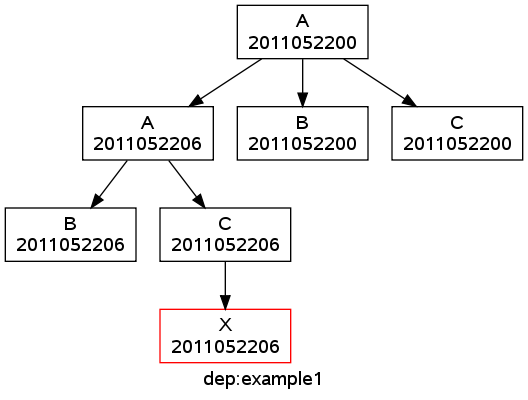
\includegraphics[width=\textwidth]{graphics/png/orig/dep-eg-1.png}
    \end{center}
\end{minipage}
\caption[Example Suite]{\scriptsize Example Suite}
\label{fig-dep-eg-1}
\end{figure}

\subsubsection{Graph String Syntax}

Multiline graph strings may contain:
\begin{myitemize}
    \item {\bf blank lines}
    \item {\bf arbitrary white space}
    \item {\bf internal comments:} following the \lstinline=#= character
    \item {\bf conditional task trigger expressions} - see below.
\end{myitemize}

\subsubsection{Interpreting Graph Strings}

Suite dependency graphs can be broken down into pairs in which the left
side (which may be a single task or family, or several that are
conditionally related) defines a trigger for the task or family on the
right. For instance the ``word graph'' {\em C triggers off B which
triggers off A} can be deconstructed into pairs {\em C triggers off B}
and {\em B triggers off A}. In this section we use only the default
trigger type, which is to trigger off the upstream task succeeding;
see~\ref{TriggerTypes} for other available triggers.

In the case of cycling tasks, the triggers defined by a graph string are
valid for cycle points matching the list of hours specified for the
graph section. For example this graph:
\lstset{language=suiterc}
\begin{lstlisting}
[scheduling]
    [[dependencies]]
        [[[T00,T12]]]
            graph = "A => B"
\end{lstlisting}
\lstset{language=transcript}
implies that B triggers off A for cycle points in which the hour matches $00$
or $12$.

To define inter-cycle dependencies, attach an offset indicator to the
left side of a pair:
\lstset{language=suiterc}
\begin{lstlisting}
[scheduling]
    [[dependencies]]
        [[[T00,T12]]]
            graph = "A[-PT12H] => B"
\end{lstlisting}
\lstset{language=transcript}
This means B[time] triggers off A[time-PT12H] (12 hours before) for cycle
points with hours matching $00$ or $12$. $time$ is implicit because this keeps
graphs clean and concise, given that the majority of tasks will typically
depend only on others with the same cycle point. Cycle point offsets can only
appear on the left of a pair, because a pairs define triggers for the right
task at cycle point $time$. However, \lstinline@A => B[-PT6H]@, which is
illegal, can be reformulated as a {\em future trigger}
\lstinline@A[+PT6H] => B@ (see~\ref{InterCyclePointTriggers}). It is also
possible to combine multiple offsets within a cycle point offset e.g.
\lstset{language=suiterc}
\begin{lstlisting}
[scheduling]
    [[dependencies]]
        [[[T00,T12]]]
            graph = "A[-P1D-PT12H] => B"
\end{lstlisting}
\lstset{language=transcript}
This means that B[Time] triggers off A[time-P1D-PT12H] (1 day and 12 hours
before).

Triggers can be chained together. This graph:
\lstset{language=suiterc}
\begin{lstlisting}
    graph = """A => B  # B triggers off A
               B => C  # C triggers off B"""
\end{lstlisting}
is equivalent to this:
\begin{lstlisting}
    graph = "A => B => C"
\end{lstlisting}
\lstset{language=transcript}

{\em Each trigger in the graph must be unique} but {\em the same task
can appear in multiple pairs or chains}. Separately defined triggers
for the same task have an AND relationship. So this:
\lstset{language=suiterc}
\begin{lstlisting}
    graph = """A => X  # X triggers off A
               B => X  # X also triggers off B"""
\end{lstlisting}
\lstset{language=transcript}
\lstset{language=suiterc}
is equivalent to this:
\begin{lstlisting}
    graph = "A & B => X"  # X triggers off A AND B
\end{lstlisting}
\lstset{language=transcript}

In summary, the branching tree structure of a dependency graph can
be partitioned into lines (in the suite.rc graph string) of pairs
or chains, in any way you like, with liberal use of internal white space
and comments to make the graph structure as clear as possible.

\begin{lstlisting}
# B triggers if A succeeds, then C and D trigger if B succeeds:
    graph = "A => B => C & D"
# which is equivalent to this:
    graph = """A => B => C
               B => D"""
# and to this:
    graph = """A => B => D
               B => C"""
# and to this:
    graph = """A => B
               B => C
               B => D"""
# and it can even be written like this:
    graph = """A => B # blank line follows:

               B => C # comment ...
               B => D"""
\end{lstlisting}

\paragraph{Handling Long Graph Lines}

Long chains of dependencies can be split into pairs:
\begin{lstlisting}
    graph = "A => B => C"
# is equivalent to this:
    graph = """A => B
               B => C"""
# BUT THIS IS AN ERROR:
    graph = """A => B => # WRONG!
               C"""      # WRONG!
\end{lstlisting}
If you have very long task names, or long conditional trigger
expressions (below) then you can use the suite.rc line continuation
marker:
\begin{lstlisting}
    graph = "A => B \
    => C"  # OK
\end{lstlisting}
Note that a line continuation marker must be the final character on
the line; it cannot be followed by trailing spaces or a comment.

\lstset{language=transcript}

\subsubsection{Graph Types}
\label{GraphTypes}

A suite definition can contain multiple graph strings that are combined
to generate the final graph.

\paragraph{One-off (Non-Cycling)}

Figure~\ref{fig-test1} shows a small suite of one-off non-cycling
tasks; these all share a single cycle point (\lstinline=1=) and don't spawn
successors (once they're all finished the suite just exits). The integer
\lstinline=1= attached to each graph node is just an arbitrary label here.
\begin{figure}
\begin{minipage}[b]{0.5\textwidth}
\lstset{language=suiterc}
\begin{lstlisting}
title = some one-off tasks
[scheduling]
    [[dependencies]]
        graph = "foo => bar & baz => qux"
\end{lstlisting}
\lstset{language=transcript}
\end{minipage}
\hfill
\begin{minipage}[b]{0.5\textwidth}
    \begin{center}
        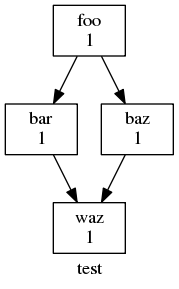
\includegraphics[width=0.25\textwidth]{graphics/png/orig/test1.png}
    \end{center}
\end{minipage}
\caption[One-off (Non-Cycling) Tasks]{\scriptsize One-off (Non-Cycling) Tasks.}
\label{fig-test1}
\end{figure}

\paragraph{Cycling Graphs}

For cycling tasks the graph section heading defines a sequence of cycle points
for which the subsequent graph section is valid. Figure~\ref{fig-test2} shows
a small suite of cycling tasks.
\begin{figure}
\begin{minipage}[b]{0.5\textwidth}
\lstset{language=suiterc}
\begin{lstlisting}
title = some cycling tasks
# (no dependence between cycle points)
[scheduling]
    [[dependencies]]
        [[[T00,T12]]]
            graph = "foo => bar & baz => qux"
\end{lstlisting}
\lstset{language=transcript}
\end{minipage}
\hfill
\begin{minipage}[b]{0.5\textwidth}
    \begin{center}
        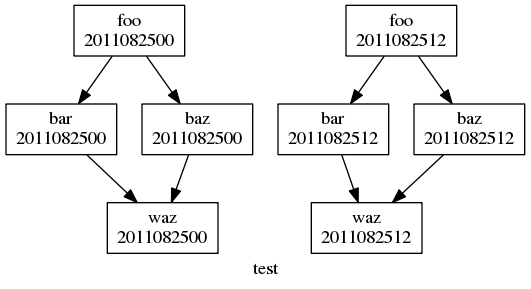
\includegraphics[width=\textwidth]{graphics/png/orig/test2.png}
    \end{center}
\end{minipage}
\caption[Cycling Tasks]{\scriptsize Cycling Tasks.}
\label{fig-test2}
\end{figure}

\subsubsection{Graph Section Headings}

Graph section headings define recurrence expressions, the graph within a graph
section heading defines a workflow at each point of the recurrence. For
example in the following scenario:

\lstset{language=suiterc}
\begin{lstlisting}
[scheduling]
    [[dependencies]]
        [[[ T06 ]]]  # A graph section heading
            graph = foo => bar
\end{lstlisting}
\lstset{language=transcript}

\lstinline=T06= means "Run every day starting at 06:00 after the
initial cycle point". Cylc allows you to start (or end) at any particular
time, repeat at whatever frequency you like, and even optionally limit the
number of repetitions.

Graph section heading can also be used with integer cycling see
\ref{IntegerCycling}.

\paragraph{Syntax Rules}

Date-time cycling information is made up of a starting {\em date-time}, an
{\em interval}, and an optional {\em limit}.

The time is assumed to be in the local time zone unless you set
\lstinline=[cylc]cycle point time zone= or \lstinline=[cylc]UTC mode=. The
calendar is assumed to be the proleptic Gregorian calendar unless you set
\lstinline=[scheduling]cycling mode=.

The syntax for representations is based on the ISO 8601 date-time standard.
This includes the representation of {\em date-time}, {\em interval}. What we
define for cylc's cycling syntax is our own optionally-heavily-condensed form
of ISO 8601 recurrence syntax. The most common full form is:
\lstinline=R[limit?]/[date-time]/[interval]=. However, we allow omitting
information that can be guessed from the context (rules below). This means
that it can be written as:
\begin{lstlisting}
R[limit?]/[date-time]
R[limit?]//[interval]
[date-time]/[interval]
R[limit?] # Special limit of 1 case
[date-time]
[interval]
\end{lstlisting}

with example graph headings for each form being:

\lstset{language=suiterc}
\begin{lstlisting}
[[[ R5/T00 ]]]           # Run 5 times at 00:00 every day
[[[ R//PT1H ]]]          # Run every hour (Note the R// is redundant)
[[[ 20000101T00Z/P1D ]]] # Run every day starting at 00:00 1st Jan 2000
[[[ R1 ]]]               # Run once at the initial cycle point
[[[ 20000101T00Z ]]]     # Run once at 00:00 1st Jan 2000
[[[ P1Y ]]]              # Run every year
\end{lstlisting}

Note that \lstinline=T00= is an example of \lstinline=[date-time]=, with an
inferred 1 day period and no limit.

Where some or all {\em date-time} information is omitted, it is inferred to
be relative to the initial date-time cycle point. For example, \lstinline=T00=
by itself would mean the next occurrence of midnight that follows, or is, the
initial cycle point. Entering \lstinline=+PT6H= would mean 6 hours after the
initial cycle point. Entering \lstinline=-P1D= would mean 1 day before the
initial cycle point. Entering no information for the {\em date-time} implies
the initial cycle point date-time itself.

Where the {\em interval} is omitted and some (but not all) {\em date-time}
information is omitted, it is inferred to be a single unit above
the largest given specific {\em date-time } unit. For example, the largest
given specific unit in \lstinline=T00= is hours, so the inferred interval is
1 day (daily), \lstinline=P1D=.

Where the {\em limit} is omitted, unlimited cycling is assumed. This will be
bounded by the final cycle point's date-time if given.

Another supported form of ISO 8601 recurrence is:
\lstinline=R[limit?]/[interval]/[date-time]=. This form uses the
{\em date-time } as the end of the cycling sequence rather than the start.
For example, \lstinline=R3/P5D/20140430T06= means:
\begin{lstlisting}
20140420T06
20140425T06
20140430T06
\end{lstlisting}

This kind of form can be used for specifying special behaviour near the end of
the suite, at the final cycle point's date-time. We can also represent this in
cylc with a collapsed form:
\begin{lstlisting}
R[limit?]/[interval]
R[limit?]//[date-time]
[interval]/[date-time]
\end{lstlisting}

So, for example, you can write:
\lstset{language=suiterc}
\begin{lstlisting}
[[[ R1//+P0D ]]]  # Run once at the final cycle point
[[[ R5/P1D ]]]    # Run 5 times, every 1 day, ending at the final
                  # cycle point
[[[ P2W/T00 ]]]   # Run every 2 weeks ending at 00:00 following
                  # the final cycle point
[[[ R//T00 ]]]    # Run every 1 day ending at 00:00 following the
                  # final cycle point
\end{lstlisting}
\lstset{language=transcript}

\paragraph{Referencing The Initial And Final Cycle Points}
\label{referencing-the-initial-and-final-cycle-points}

For convenience the caret and dollar symbols may be used as shorthand for the
initial and final cycle points. Using this shorthand you can write:

\lstset{language=suiterc}
\begin{lstlisting}
[[[ R1/^+PT12H ]]]  # Repeat once 12 hours after the initial cycle point
                    # R[limit]/[date-time]
                    # Equivalent to [[[ R1/+PT12H ]]]
[[[ R1/$ ]]]        # Repeat once at the final cycle point
                    # R[limit]/[date-time]
                    # Equivalent to [[[ R1//+P0D ]]]
[[[ $-P2D/PT3H ]]]  # Repeat 3 hourly starting two days before the
                    # [date-time]/[interval]
                    # final cycle point
\end{lstlisting}
\lstset{language=transcript}

Note that there can be multiple ways to write the same headings, for instance
the following all run once at the final cycle point:

\lstset{language=suiterc}
\begin{lstlisting}
[[[ R1/P0Y ]]]      # R[limit]/[interval]
[[[ R1/P0Y/$ ]]]    # R[limit]/[interval]/[date-time]
[[[ R1/$ ]]]        # R[limit]/[date-time]
\end{lstlisting}
\lstset{language=transcript}

\paragraph{Excluding Dates}
\label{excluding-dates}
\lstset{language=suiterc}

Datetimes can be excluded from a recurrence by an exclamation mark for example
\lstinline=[[[ PT1D!20000101 ]]]= means run daily except on the
first of January 2000.

This syntax can only be used to exclude one datetime from a recurrence. Note
that the \lstinline=^= and \lstinline=$= symbols (shorthand for the initial
and final cycle points) are both datetimes so \lstinline=[[[ T12!$-PT1D ]]]=
is valid.

If using a run limit in combination with an exclusion, the heading might not
run the number of times specified in the limit. For example in the following
suite \lstinline=foo= will only run once as its second run has been excluded.

\begin{lstlisting}
[scheduling]
    initial cycle point = 20000101T00Z
    final cycle point = 20000105T00Z
    [[dependencies]]
        [[[ R2/P1D!20000102 ]]]
            graph = foo
\end{lstlisting}
\lstset{language=transcript}

\paragraph{How Multiple Graph Strings Combine}
\label{HowMultipleGraphStringsCombine}

For a cycling graph with multiple validity sections for different
hours of the day, the different sections {\em add} to generate the
complete graph. Different graph sections can overlap (i.e.\ the same
hours may appear in multiple section headings) and the same tasks may
appear in multiple sections, but individual dependencies should be
unique across the entire graph. For example, the following graph defines
a duplicate prerequisite for task C:
\lstset{language=suiterc}
\begin{lstlisting}
[scheduling]
    [[dependencies]]
        [[[T00,T06,T12,T18]]]
            graph = "A => B => C"
        [[[T06,T18]]]
            graph = "B => C => X"
            # duplicate prerequisite: B => C already defined at T06, T18
\end{lstlisting}
\lstset{language=transcript}
This does not affect scheduling, but for the sake of clarity and brevity
the graph should be written like this:
\lstset{language=suiterc}
\begin{lstlisting}
[scheduling]
    [[dependencies]]
        [[[T00,T06,T12,T18]]]
            graph = "A => B => C"
        [[[T06,T18]]]
            # X triggers off C only at 6 and 18 hours
            graph = "C => X"
\end{lstlisting}
\lstset{language=transcript}

\paragraph{Advanced Examples}
\label{AdvancedCycling}

The following examples show the various ways of writing graph headings in cylc.
\lstset{language=suiterc}
\begin{lstlisting}
[[[ R1 ]]]         # Run once at the initial cycle point
[[[ P1D ]]]        # Run every day starting at the initial cycle point
[[[ PT5M ]]]       # Run every 5 minutes starting at the initial cycle
                   # point
[[[ T00/P2W ]]]    # Run every 2 weeks starting at 00:00 after the
                   # initial cycle point
[[[ +P5D/P1M ]]]   # Run every month, starting 5 days after the initial
                   # cycle point
[[[ R1/T06 ]]]     # Run once at 06:00 after the initial cycle point
[[[ R1/P0Y ]]]     # Run once at the final cycle point
[[[ R1/$ ]]]       # Run once at the final cycle point (alternative
                   # form)
[[[ R1/$-P3D ]]]   # Run once three days before the final cycle point
[[[ R3/T0830 ]]]   # Run 3 times, every day at 08:30 after the initial
                   # cycle point
[[[ R3/01T00 ]]]   # Run 3 times, every month at 00:00 on the first
                   # of the month after the initial cycle point
[[[ R5/W-1/P1M ]]] # Run 5 times, every month starting on Monday
                   # following the initial cycle point
[[[ T00!^ ]]]      # Run at the first occurrence of T00 that isn't the
                   # initial cycle point
[[[ PT1D!20000101 ]]]  # Run every day days excluding 1st Jan 2000
[[[ 20140201T06/P1D ]]]    # Run every day starting at 20140201T06
[[[ R1/min(T00,T06,T12,T18) ]]]  # Run once at the first instance
                                 # of either T00, T06, T12 or T18
                                 # starting at the initial cycle
                                 # point
\end{lstlisting}
\lstset{language=transcript}

\paragraph{Advanced Starting Up}
\label{AdvancedStartingUp}

Dependencies that are only valid at the initial cycle point can be written
using the \lstinline=R1= notation (e.g. as
in~\ref{initial-non-repeating-r1-tasks}. For example:
\lstset{language=suiterc}
\begin{lstlisting}
[cylc]
    UTC mode = True
[scheduling]
    initial cycle point = 20130808T00
    final cycle point = 20130812T00
    [[dependencies]]
        [[[R1]]]
            graph = "prep => foo"
        [[[T00]]]
            graph = "foo[-P1D] => foo => bar"
\end{lstlisting}
\lstset{language=transcript}

In the example above, \lstinline=R1= implies \lstinline=R1/20130808T00=, so
\lstinline=prep= only runs once at that cycle point (the initial cycle point).
At that cycle point, \lstinline=foo= will have a dependence on
\lstinline=prep= - but not at subsequent cycle points.

However, it is possible to have a suite that has multiple effective initial
cycles - for example, one starting at \lstinline=T00= and another starting
at \lstinline=T12=. What if they need to share an initial task?

Let's suppose that we add the following section to the suite example above:
\lstset{language=suiterc}
\begin{lstlisting}
[cylc]
    UTC mode = True
[scheduling]
    initial cycle point = 20130808T00
    final cycle point = 20130812T00
    [[dependencies]]
        [[[R1]]]
            graph = "prep => foo"
        [[[T00]]]
            graph = "foo[-P1D] => foo => bar"
        [[[T12]]]
            graph = "baz[-P1D] => baz => qux"
\end{lstlisting}
\lstset{language=transcript}

We'll also say that there should be a starting dependence between
\lstinline=prep= and our new task \lstinline=baz= - but we still want to have
a single \lstinline=prep= task, at a single cycle.

We can write this using a special case of the \lstinline=task[-interval]= syntax -
if the interval is null, this implies the task at the initial cycle point.

For example, we can write our suite like~\ref{fig-test4}.

\begin{figure}
\begin{minipage}[b]{0.5\textwidth}
\lstset{language=suiterc}
\begin{lstlisting}
[cylc]
    UTC mode = True
[scheduling]
    initial cycle point = 20130808T00
    final cycle point = 20130812T00
    [[dependencies]]
        [[[R1]]]
            graph = "prep"
        [[[R1/T00]]]
# ^ implies the initial cycle point:
     graph = "prep[^] => foo"
        [[[R1/T12]]]
# ^ is initial cycle point, as above:
     graph = "prep[^] => baz"
        [[[T00]]]
     graph = "foo[-P1D] => foo => bar"
        [[[T12]]]
     graph = "baz[-P1D] => baz => qux"
[visualization]
    initial cycle point = 20130808T00
    final cycle point = 20130810T00
    [[node attributes]]
        foo = "color=red"
        bar = "color=orange"
        baz = "color=green"
        qux = "color=blue"
\end{lstlisting}
\lstset{language=transcript}
\end{minipage}
\hfill
\begin{minipage}[b]{0.5\textwidth}
    \begin{center}
        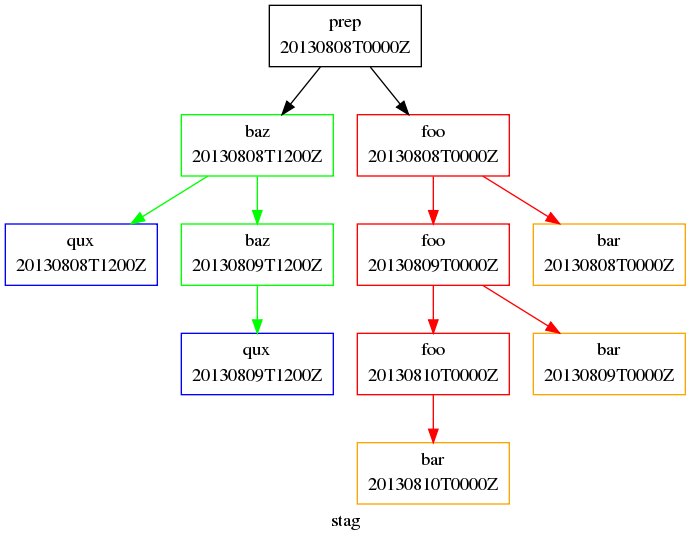
\includegraphics[width=\textwidth]{graphics/png/orig/test4.png}
    \end{center}
\end{minipage}
\caption[Staggered Start Suite]{\scriptsize Staggered Start Suite}
\label{fig-test4}
\end{figure}

This neatly expresses what we want - a task running at the initial cycle point
that has one-off dependencies with other task sets at different cycles.

\begin{figure}
\begin{minipage}[h]{0.5\textwidth}
\lstset{language=suiterc}
\begin{lstlisting}
[cylc]
    UTC mode = True
[scheduling]
    initial cycle point = 20130808T00
    final cycle point = 20130808T18
    [[dependencies]]
        [[[R1]]]
            graph = "setup_foo => foo"
        [[[+PT6H/PT6H]]]
            graph = """
                foo[-PT6H] => foo
                foo => bar
            """
[visualization]
    initial cycle point = 20130808T00
    final cycle point = 20130808T18
    [[node attributes]]
        foo = "color=red"
        bar = "color=orange"
\end{lstlisting}
\lstset{language=transcript}
\end{minipage}
\hfill
\begin{minipage}[h]{0.5\textwidth}
    \begin{center}
        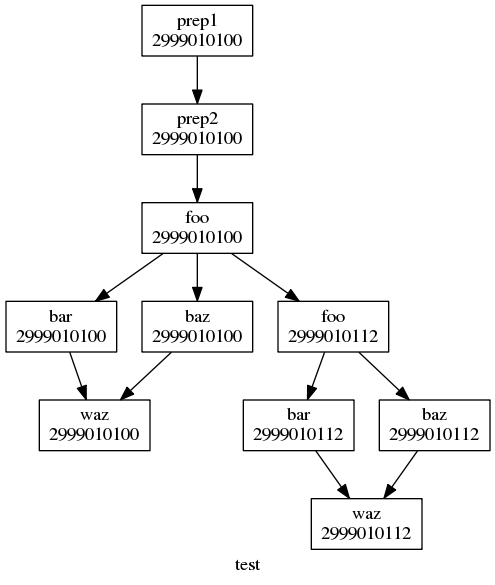
\includegraphics[width=\textwidth]{graphics/png/orig/test5.png}
    \end{center}
\end{minipage}
\caption[Restricted First Cycle Point Suite]{
    \scriptsize Restricted First Cycle Point Suite}
\label{fig-test5}
\end{figure}


A different kind of requirement is displayed in Figure \ref{fig-test5}.
Usually, we want to specify additional tasks and dependencies at the initial
cycle point. What if we want our first cycle point to be entirely special, with
some tasks missing compared to subsequent cycle points?

In Figure \ref{fig-test5}, \lstinline=bar= will not be run at the initial
cycle point, but will still run at subsequent cycle points.
\lstinline=[[[+PT6H/PT6H]]]= means start at \lstinline=+PT6H= (6 hours after
the initial cycle point) and then repeat every \lstinline=PT6H= (6 hours).

Some suites may have staggered start-up sequences where different tasks need
running once but only at specific cycle points, potentially due to differing
data sources at different cycle points with different possible initial cycle
points. To allow this cylc provides a \lstinline=min( )= function that can be
used as follows:

\lstset{language=suiterc}
\begin{lstlisting}
[cylc]
    UTC mode = True
[scheduling]
    initial cycle point = 20100101T03
    [[dependencies]]
        [[[R1/min(T00,T12)]]]
            graph = "prep1 => foo"
        [[[R1/min(T06,T18)]]]
            graph = "prep2 => foo"
        [[[T00,T06,T12,T18]]]
            graph = "foo => bar"

\end{lstlisting}
\lstset{language=transcript}


In this example the initial cycle point is \lstinline=20100101T03=, so the
\lstinline=prep1= task will run once at \lstinline=20100101T12= and the
\lstinline=prep2= task will run once at \lstinline=20100101T06= as these are
the first cycle points after the initial cycle point in the respective
\lstinline=min( )= entries.


\paragraph{Integer Cycling}
\label{IntegerCycling}

In addition to non-repeating and date-time cycling workflows, cylc can do
integer cycling for repeating workflows that are not date-time based.

To construct an integer cycling suite, set
\lstinline@[scheduling]cycling mode = integer@, and specify integer values for
the initial and (optional) final cycle points. The notation for intervals,
offsets, and recurrences (sequences) is similar to the date-time cycling
notation, except for the simple integer values.

The full integer recurrence expressions supported are:
\begin{myitemize}
    \item \lstinline@Rn/start-point/interval # e.g. R3/1/P2@
    \item \lstinline@Rn/interval/end-point # e.g. R3/P2/9@
\end{myitemize}
But, as for date-time cycling, sequence start and end points can be omitted
where suite initial and final cycle points can be assumed. Some examples:

\lstset{language=suiterc}
\begin{lstlisting}
[[[ R1 ]]]        # Run once at the initial cycle point
                  # (short for R1/initial-point/?)
[[[ P1 ]]]        # Repeat with step 1 from the initial cycle point
                  # (short for R/initial-point/P1)
[[[ P5 ]]]        # Repeat with step 5 from the initial cycle point
                  # (short for R/initial-point/P5)
[[[ R2//P2 ]]]    # Run twice with step 3 from the initial cycle point
                  # (short for R2/initial-point/P2)
[[[ R/+P1/P2 ]]]  # Repeat with step 2, from 1 after the initial cycle point
[[[ R2/P2 ]]]     # Run twice with step 2, to the final cycle point
                  # (short for R2/P2/final-point)
[[[ R1/P0 ]]]     # Run once at the final cycle point
                  # (short for R1/P0/final-point)
\end{lstlisting}

\subparagraph{Example}

The tutorial illustrates integer cycling in~\ref{TutInteger}, and
\lstinline=$CYLC_DIR/examples/satellite/= is a
self-contained example of a realistic use for integer cycling. It simulates
the processing of incoming satellite data: each new dataset arrives after a
random (as far as the suite is concerned) interval, and is labeled by an
arbitrary (as far as the suite is concerned) ID in the filename. A task called
\lstinline=get_data= at the top of the repeating workflow waits on the next
dataset and, when it finds one, moves it to a cycle-point-specific shared
workspace for processing by the downstream tasks. When \lstinline=get_data.1=
finishes, \lstinline=get_data.2= triggers and begins waiting for the next
dataset at the same time as the downstream tasks in cycle point 1 are
processing the first one, and so on. In this way multiple datasets can be
processed at once if they happen to come in quickly. A single shutdown task
runs at the end of the final cycle to collate results. The suite graph is
shown in Figure~\ref{fig-satellite}.

\begin{figure}
    \begin{center}
        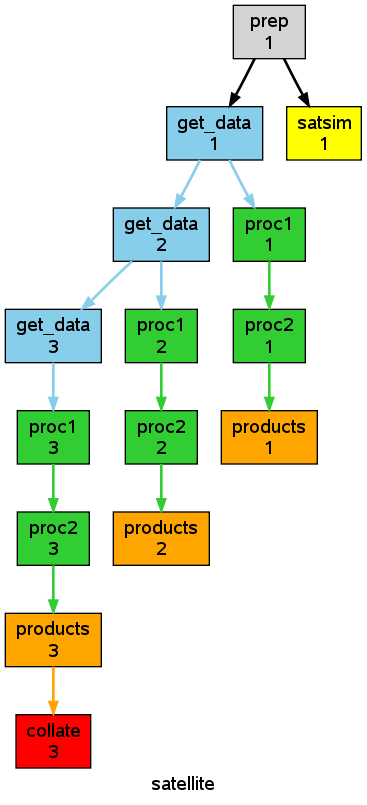
\includegraphics[width=0.4\textwidth]{graphics/png/orig/satellite.png}
    \end{center}
    \caption{The \lstinline=examples/satellite= integer suite}
\label{fig-satellite}
\end{figure}

\subparagraph{Advanced Integer Cycling Syntax}

The same syntax used to reference the initial and final cycle points
introduced in~\ref{referencing-the-initial-and-final-cycle-points}) for
use with datetime cycling can also be used for integer cycling. For
example you can write:

\lstset{language=suiterc}
\begin{lstlisting}
[[[ R1/^ ]]]     # Run once at the initial cycle point
[[[ R1/$ ]]]     # Run once at the final cycle point
[[[ R3/^/P2 ]]]  # Run three times with step two starting at the
                 # initial cycle point
\end{lstlisting}
\lstset{language=transcript}

Likewise the syntax introduced in~\ref{excluding-dates} for excluding
a particular point from a recurrence also works for integer cycling. For
example:

\lstset{language=suiterc}
\begin{lstlisting}
[[[ R/P4!8 ]]]       # Run with step 4, to the final cycle point
                     # but not at point 8
[[[ R3/3/P2!5 ]]]    # Run with step 2 from point 3 but not at
                     # point 5
[[[ R/+P1/P6!14 ]]]  # Run with step 6 from 1 step after the
                     # initial cycle point but not at point 14
\end{lstlisting}
\lstset{language=transcript}


\subsubsection{Trigger Types}
\label{TriggerTypes}

\lstset{language=suiterc}

Trigger type, indicated by {\em:type} after the upstream task (or family)
name, determines what kind of event results in the downstream task (or
family) triggering.

\paragraph{Success Triggers}

The default, with no trigger type specified, is to trigger off the
upstream task succeeding:
\begin{lstlisting}
# B triggers if A SUCCEEDS:
    graph = "A => B"
\end{lstlisting}
For consistency and completeness, however, the success trigger can be explicit:
\begin{lstlisting}
# B triggers if A SUCCEEDS:
    graph = "A => B"
# or:
    graph = "A:succeed => B"
\end{lstlisting}

\paragraph{Failure Triggers}

To trigger off the upstream task reporting failure:
\begin{lstlisting}
# B triggers if A FAILS:
    graph = "A:fail => B"
\end{lstlisting}
{\em Suicide triggers} can be used to remove task \lstinline=B= here if
\lstinline=A= does not fail, see~\ref{SuicideTriggers}.

\paragraph{Start Triggers}

To trigger off the upstream task starting to execute:
\begin{lstlisting}
# B triggers if A STARTS EXECUTING:
    graph = "A:start => B"
\end{lstlisting}
This can be used to trigger tasks that monitor other tasks once they
(the target tasks) start executing. Consider a long-running forecast model,
for instance, that generates a sequence of output files as it runs. A
postprocessing task could be launched with a start trigger on the model
(\lstinline@model:start => post@) to process the model output as it
becomes available. Note, however, that there are several alternative
ways of handling this scenario: both tasks could be triggered at the
same time (\lstinline@foo => model & post@), but depending on
external queue delays this could result in the monitoring task starting
to execute first; or a different postprocessing task could be
triggered off a message output for each data file
(\lstinline@model:out1 => post1@ etc.; see~\ref{MessageTriggers}), but this
may not be practical if the
number of output files is large or if it is difficult to add cylc
messaging calls to the model.

\paragraph{Finish Triggers}

To trigger off the upstream task succeeding or failing, i.e.\ finishing
one way or the other:
\begin{lstlisting}
# B triggers if A either SUCCEEDS or FAILS:
    graph = "A | A:fail => B"
# or
    graph = "A:finish => B"
\end{lstlisting}

\paragraph{Message Triggers}
\label{MessageTriggers}

Tasks can also trigger off custom output messages. These must be registered in
the \lstinline=[runtime]= section of the emitting task, and reported using the
\lstinline=cylc message= command in task scripting. The graph trigger notation
refers to the item name of the registered output message.
The example suite \lstinline=$CYLC_DIR/examples/message-triggers= illustrates
message triggering.

\lstset{language=suiterc}
\lstinputlisting{../examples/message-triggers/suite.rc}

\paragraph{Job Submission Triggers}

It is also possible to trigger off a task submitting, or failing to submit:
\begin{lstlisting}
# B triggers if A submits successfully:
    graph = "A:submit => B"
# D triggers if C fails to submit successfully:
    graph = "C:submit-fail => D"
\end{lstlisting}

A possible use case for submit-fail triggers: if a task goes into the
submit-failed state, possibly after several job submission retries,
another task that inherits the same runtime but sets a different job
submission method and/or host could be triggered to, in effect, run the
same job on a different platform.


\paragraph{Conditional Triggers}

AND operators (\lstinline=&=) can appear on both sides of an arrow. They
provide a concise alternative to defining multiple triggers separately:
\begin{lstlisting}
# 1/ this:
    graph = "A & B => C"
# is equivalent to:
    graph = """A => C
               B => C"""
# 2/ this:
    graph = "A => B & C"
# is equivalent to:
    graph = """A => B
               A => C"""
# 3/ and this:
    graph = "A & B => C & D"
# is equivalent to this:
    graph = """A => C
               B => C
               A => D
               B => D"""
\end{lstlisting}

OR operators (\lstinline=|=) which result in true conditional triggers,
can only appear on the left,\footnote{An OR
operator on the right doesn't make much sense: if ``B or C'' triggers
off A, what exactly should cylc do when A finishes?}
\begin{lstlisting}
# C triggers when either A or B finishes:
    graph = "A | B => C"
\end{lstlisting}

Forecasting suites typically have simple conditional
triggering requirements, but any valid conditional expression can be
used, as shown in Figure~\ref{fig-conditional}
(conditional triggers are plotted with open arrow heads).
\begin{figure}
\begin{minipage}[b]{0.5\textwidth}
\lstset{language=suiterc}
\begin{lstlisting}
        graph = """
# D triggers if A or (B and C) succeed
A | B & C => D
# just to align the two graph sections
D => W
# Z triggers if (W or X) and Y succeed
(W|X) & Y => Z
                """
\end{lstlisting}
\lstset{language=transcript}
\end{minipage}
\hfill
\begin{minipage}[b]{0.5\textwidth}
    \begin{center}
        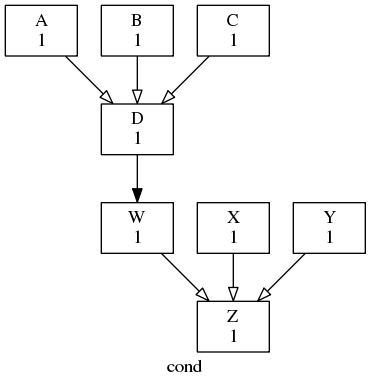
\includegraphics[width=0.5\textwidth]{graphics/png/orig/conditional-triggers.png}
    \end{center}
\end{minipage}
\caption[Conditional Triggers] {\scriptsize
Conditional triggers are plotted with open arrow heads.}
\label{fig-conditional}
\end{figure}

\paragraph{Suicide Triggers}
\label{SuicideTriggers}

Suicide triggers take tasks out of the suite. This can be used for
automated failure recovery. The suite.rc listing and accompanying
graph in Figure~\ref{fig-suicide} show how to define a chain of failure
recovery tasks
that trigger if they're needed but otherwise remove themselves from the
suite (you can run the {\em AutoRecover.async} example suite to see how
this works). The dashed graph edges ending in solid dots indicate
suicide triggers, and the open arrowheads indicate conditional triggers
as usual. Suicide triggers are ignored by default in the graph view, unless you toggle them on with {\em View} -> {\em Options} -> {\em Ignore Suicide Triggers}.

\begin{figure}
\begin{minipage}[b]{0.5\textwidth}
\lstset{language=suiterc}
\begin{lstlisting}
title = automated failure recovery
description = """
Model task failure triggers diagnosis
and recovery tasks, which take themselves
out of the suite if model succeeds. Model
post processing triggers off model OR
recovery tasks.
              """
[scheduling]
    [[dependencies]]
        graph = """
pre => model
model:fail => diagnose => recover
model => !diagnose & !recover
model | recover => post
                """
[runtime]
    [[model]]
        # UNCOMMENT TO TEST FAILURE:
        # script = /bin/false
\end{lstlisting}
\lstset{language=transcript}
\end{minipage}
\hfill
\begin{minipage}[b]{0.5\textwidth}
    \begin{center}
        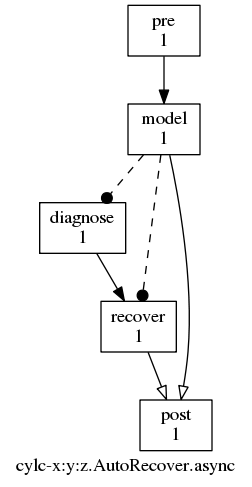
\includegraphics[width=0.5\textwidth]{graphics/png/orig/suicide.png}
    \end{center}
\end{minipage}
\caption[Automated failure recovery via suicide triggers] {\scriptsize
Automated failure recovery via suicide triggers.}
\label{fig-suicide}
\end{figure}

Note that multiple suicide triggers combine in the same way as other triggers, so this:
\begin{lstlisting}
foo => !baz
bar => !baz
\end{lstlisting}
is equivalent to this:
\begin{lstlisting}
foo & bar => !baz
\end{lstlisting}
i.e.\ both \lstinline=foo= and \lstinline=bar= must succeed for
\lstinline=baz= to be taken out of the suite. If you really want a task
to be taken out if any one of several events occurs then be careful to
write it that way:
\begin{lstlisting}
foo | bar => !baz
\end{lstlisting}

A word of warning on the meaning of ``bare suicide triggers''. Consider
the following suite:
\lstset{language=suiterc}
\begin{lstlisting}
[scheduling]
    [[dependencies]]
        graph = "foo => !bar"
\end{lstlisting}
Task \lstinline=bar= has a suicide trigger but no normal prerequisites
(a suicide trigger is not a task triggering prerequisite, it is a task
removal prerequisite) so this is entirely equivalent to:
\lstset{language=suiterc}
\begin{lstlisting}
[scheduling]
    [[dependencies]]
        graph = """
            foo & bar
           foo => !bar
                """
\end{lstlisting}
In other words both tasks will trigger immediately, at the same time,
and then \lstinline=bar= will be removed if \lstinline=foo= succeeds.

If an active task proxy (currently in the submitted or running states)
is removed from the suite by a suicide trigger, a warning will be logged.

\paragraph{Family Triggers}
\label{FamilyTriggers}

Families defined by the namespace inheritance hierarchy
(~\ref{NIORP}) can be used in the graph trigger whole groups of
tasks at the same time (e.g.\ forecast model ensembles and groups of
tasks for processing different observation types at the same time) and
for triggering downstream tasks off families as a whole. Higher level
families, i.e.\ families of families, can also be used, and are reduced
to the lowest level member tasks. Note that tasks can also trigger off
individual family members if necessary.

To trigger an entire task family at once:
\begin{lstlisting}
[scheduling]
    [[dependencies]]
        graph = "foo => FAM"
[runtime]
    [[FAM]]    # a family (because others inherit from it)
    [[m1,m2]]  # family members (inherit from namespace FAM)
        inherit = FAM
\end{lstlisting}
This is equivalent to:
\begin{lstlisting}
[scheduling]
    [[dependencies]]
        graph = "foo => m1 & m2"
[runtime]
    [[FAM]]
    [[m1,m2]]
        inherit = FAM
\end{lstlisting}

To trigger other tasks off families we have to specify whether
to triggering off {\em all members} starting, succeeding, failing,
or finishing, or off {\em any} members (doing the same). Legal family
triggers are thus:

\begin{lstlisting}
[scheduling]
    [[dependencies]]
        graph = """
      # all-member triggers:
    FAM:start-all => one
    FAM:succeed-all => one
    FAM:fail-all => one
    FAM:finish-all => one
      # any-member triggers:
    FAM:start-any => one
    FAM:succeed-any => one
    FAM:fail-any => one
    FAM:finish-any => one
                """
\end{lstlisting}

Here's how to trigger downstream processing after if one or more family
members succeed, but only after all members have finished (succeeded or
failed):

\begin{lstlisting}
[scheduling]
    [[dependencies]]
        graph = """
    FAM:finish-all & FAM:succeed-any => foo
                """
\end{lstlisting}

\paragraph{Writing Efficient Inter-Family Triggering}
\label{EfficientInterFamilyTriggering}

While cylc allows writing dependencies between two families it is important to
consider the number of dependencies this will generate. In the following
example, each member of \lstinline=FAM2= has dependencies pointing at all the
members of \lstinline=FAM1=.

\begin{lstlisting}
[scheduling]
    [[dependencies]]
        graph = """
    FAM1:succeed-any => FAM2
                """
\end{lstlisting}

Expanding this out, you generate \lstinline=N * M= dependencies, where
\lstinline=N= is the number of members of \lstinline=FAM1= and \lstinline=M= is
the number of members of \lstinline=FAM2=. This can result in high memory use
as the number of members of these families grows, potentially rendering the
suite impractical for running on some systems.

You can greatly reduce the number of dependencies generated in these situations
by putting dummy tasks in the graphing to represent the state of the family you
want to trigger off. For example, if \lstinline=FAM2= should trigger off any
member of \lstinline=FAM1= succeeding you can create a dummy task
\lstinline=FAM1_succeed_any_marker= and place a dependency on it as follows:

\begin{lstlisting}
[scheduling]
    [[dependencies]]
        graph = """
    FAM1:succeed-any => FAM1_succeed_any_marker => FAM2
                """
[runtime]
...
    [[FAM1_succeed_any_marker]]
        script = true
...
\end{lstlisting}

This graph generates only \lstinline=N + M= dependencies, which takes
significantly less memory and CPU to store and evaluate.

\paragraph{Inter-Cycle Triggers}
\label{InterCyclePointTriggers}

Typically most tasks in a suite will trigger off others in the same
cycle point, but some may depend on others with other cycle points.
This notably applies to warm-cycled forecast models, which depend on
their own previous instances (see below); but other kinds of inter-cycle
dependence are possible too.\footnote{In NWP forecast analysis
suites parts of the observation processing and data assimilation
subsystem will typically also depend on model background fields
generated by the previous forecast.} Here's how to express this
kind of relationship in cylc:
\begin{lstlisting}
[dependencies]
    [[PT6H]]
        # B triggers off A in the previous cycle point
        graph = "A[-PT6H] => B"
\end{lstlisting}
inter-cycle and trigger type (or message trigger) notation can be
combined:
\begin{lstlisting}
    # B triggers if A in the previous cycle point fails:
    graph = "A[-PT6H]:fail => B"
\end{lstlisting}

At suite start-up inter-cycle triggers refer to a previous cycle point
that does not exist. This does not cause the dependent task to wait
indefinitely, however, because cylc ignores triggers that reach back
beyond the initial cycle point. That said, the presence of an
inter-cycle trigger does normally imply that something special has to
happen at start-up. If a model depends on its own previous instance for
restart files, for instance, then an initial set of restart files has to be
generated somehow or the first model task will presumably fail with
missing input files. There are several ways to handle this in cylc
using different kinds of one-off (non-cycling) tasks that run at suite
start-up. They are illustrated in the Tutorial
(\ref{TutInterCyclePointTriggers}); to summarize here briefly:

\begin{myitemize}
    \item \lstinline=R1= tasks (recommended):
\lstset{language=suiterc}
\begin{lstlisting}
[scheduling]
    [[dependencies]]
        [[[R1]]]
            graph = "prep"
        [[[R1/T00,R1/T12]]]
            graph = "prep[^] => foo"
        [[[T00,T12]]]
            graph = "foo[-PT12H] => foo => bar"
\end{lstlisting}

\end{myitemize}
\lstset{language=transcript}

\lstinline=R1=, or \lstinline=R1/date-time= tasks are the recommended way to
specify unusual start up conditions. They allow you to specify a clean
distinction between the dependencies of initial cycles and the dependencies
of the subsequent cycles.

Initial tasks can be used for real model cold-start processes, whereby a
warm-cycled model at any given cycle point can in principle have its inputs
satisfied by a previous instance of itself, {\em or} by an initial task with
(nominally) the same cycle point.

In effect, the \lstinline=R1= task masquerades as the previous-cycle-point trigger
of its associated cycling task. At suite start-up initial tasks will
trigger the first cycling tasks, and thereafter the inter-cycle trigger
will take effect.

If a task has a dependency on another task in a different cycle point, the
dependency can be written using the \lstinline=[offset]= syntax such as
\lstinline=[-PT12H]= in \lstinline@foo[-PT12H] => foo@. This means that
\lstinline=foo= at the current cycle point depends on a previous instance of
 \lstinline=foo= at 12 hours before the current cycle point. Unlike the
 cycling section headings (e.g. \lstinline=[[[T00,T12]]]=), dependencies
 assume that relative times are relative to the current cycle point, not the
 initial cycle point.

However, it can be useful to have specific dependencies on tasks at or near
the initial cycle point. You can switch the context of the offset to be
the initial cycle point by using the caret symbol: \lstinline=^=.

For example, you can write \lstinline=foo[^]= to mean foo at the initial
cycle point, and \lstinline=foo[^+PT6H]= to mean foo 6 hours after the initial
cycle point. Usually, this kind of dependency will only apply in a limited
number of cycle points near the start of the suite, so you may want to write
it in \lstinline=R1=-based cycling sections. Here's the example inter-cycle
\lstinline=R1= suite from above again.

\lstset{language=suiterc}
\begin{lstlisting}
[scheduling]
    [[dependencies]]
        [[[R1]]]
            graph = "prep"
        [[[R1/T00,R1/T12]]]
            graph = "prep[^] => foo"
        [[[T00,T12]]]
            graph = "foo[-PT12H] => foo => bar"
\end{lstlisting}
\lstset{language=transcript}

You can see there is a dependence on the initial \lstinline=R1= task
\lstinline=prep= for \lstinline=foo= at the first \lstinline=T00= cycle point,
and at the first \lstinline=T12= cycle point. Thereafter, \lstinline=foo= just
depends on its previous (12 hours ago) instance.

\paragraph{Special Sequential Tasks}
\label{SequentialTasks}

If a cycling task does not generate files required by its own successor,
then successive instances can run in parallel if the opportunity arises.
However, if such a task would interfere with its own siblings for
internal reasons (e.g.\ use of a hardwired non cycle dependent
temporary file or similar) then it can be forced to run sequentially.
This can be done with explicit inter-cycle triggers in the graph:
\lstset{language=suiterc}
\begin{lstlisting}
[scheduling]
    [[dependencies]]
        [[[T00,T12]]]
            graph = "foo[-PT12H] => foo => bar"
\end{lstlisting}
or by declaring the task to be {\em sequential}:
\lstset{language=suiterc}
\begin{lstlisting}
[scheduling]
    [[special tasks]]
        sequential = foo
    [[dependencies]]
        [[[T00,T12]]]
            graph = "foo => bar"
\end{lstlisting}

The {\em sequential} declaration also results in each instance of
\lstinline=foo= triggering off its own predecessor, exactly as in
the explicit version. The only difference is that implicit triggers will
not appear in graph visualizations. The implicit version can also be
considerably simpler when the task appears in multiple graph sections or
in a non-uniform cycling sequence: this suite:
\lstset{language=suiterc}
\begin{lstlisting}
[scheduling]
    [[special tasks]]
        sequential = foo
    [[dependencies]]
        [[[T00,T03,T11]]]
            graph = "foo => bar"
\end{lstlisting}
is equivalent to this one:
\lstset{language=suiterc}
\begin{lstlisting}
[scheduling]
    [[dependencies]]
        [[[T00,T03,T11]]]
            graph = "foo => bar"
        [[[T00]]]
            graph = "foo[-PT13H] => foo"
        [[[T03]]]
            graph = "foo[-PT3H] => foo"
        [[[T11]]]
            graph = "foo[-PT8H] => foo"
\end{lstlisting}


\paragraph{Future Triggers}

Cylc also supports inter-cycle triggering off tasks ``in the future'' (with
respect to cycle point):
\begin{lstlisting}
[[dependencies]]
    [[[T00,T06,T12,T18]]]
        graph = """
    # A runs in this cycle:
            A
    # B in this cycle triggers off A in the next cycle.
            A[PT6H] => B
        """
\end{lstlisting}
(Recall that \lstinline=A[t+PT6H]= can run before B[t] because tasks in cylc
have private cycle points). Future triggers present a problem at the suite
shutdown rather than at start-up. Here, \lstinline=B= at the final cycle
point wants to trigger off an instance of \lstinline=A= that will never exist
because it is beyond the suite stop point. Consequently cylc prevents tasks
from spawning successors that depend on other tasks beyond the stop point.

\paragraph{Clock Triggers}
\label{ClockTriggerTasks}

In addition to depending on other tasks (and on external events -
see~\ref{ExternalTriggers}) tasks can depend on the wall clock: specifically,
they can trigger off a wall clock time expressed as an offset from their own
cycle point:
\lstset{language=suiterc}
\begin{lstlisting}
[scheduling]
    [[special tasks]]
        clock-trigger = foo(PT2H)
    [[dependencies]]
        [[[T00]]]
            graph = foo
\end{lstlisting}
Here, \lstinline=foo[2015-08-23T00]= would trigger (other dependencies allowing)
when the wall clock time reaches \lstinline=2015-08-23T02=. Clock-trigger
offsets are normally positive, to trigger some time {\em after} the wall-clock
time is equal to task cycle point.

Clock-triggers have no effect on scheduling if the suite is running sufficiently
far behind the clock (e.g.\ after a delay, or because it is processing archived
historical data) that the trigger times, which are relative to task cycle
point, have already passed.

\paragraph{Clock-Expire Triggers}
\label{ClockExpireTasks}

Tasks can be configured to {\em expire} - i.e.\ to skip job submission and
enter the {\em expired} state - if they are too far behind the wall clock when
they become ready to run, and other tasks can trigger off this. As a possible
use case, consider a cycling task that copies the latest of a set of files to
overwrite the previous set: if the task is delayed by more than one cycle there
may be no point in running it because the freshly copied files will just be
overwritten immediately by the next task instance as the suite catches back up
to real time operation. Clock-expire tasks are configured like clock-trigger
tasks, with a date-time offset relative to cycle point (\ref{ClockExpireRef}).
The offset should be positive to make the task expire if the wall-clock time
has gone beyond the cycle point. Triggering off an expired task typically
requires suicide triggers to remove the workflow that runs if the task has not
expired. Here a task called \lstinline=copy= expires, and its downstream
workflow is skipped, if it is more than one day behind the wall-clock (see also
\lstinline=examples/clock-expire=):
\lstset{language=suiterc}
\begin{lstlisting}
[cylc]
   cycle point format = %Y-%m-%dT%H
[scheduling]
    initial cycle point = 2015-08-15T00
    [[special tasks]]
        clock-expire = copy(-P1D)
    [[dependencies]]
        [[[P1D]]]
            graph = """
        model[-P1D] => model => copy => proc
              copy:expired => !proc"""
\end{lstlisting}

\paragraph{External Triggers}
\label{ExternalTriggers}

In addition to depending on other tasks (and on the wall clock -
see~\ref{ClockTriggerTasks}) tasks can trigger off events reported by an
external system. For example, an external process could detect incoming data
on an ftp server, and then notify a suite containing a task to retrieve the
new data for processing. This is an alternative to long-running tasks that poll
for external events.

Note that cylc does not currently support triggering off ``filesystem events''
(e.g.\ \lstinline=inotify= on Linux). However, external watcher processes can
use filesystem events to detect triggering conditions, if that is appropriate,
before notifying a suite with our general external event system.

The external triggering process must call \lstinline=cylc ext-trigger= with the
name of the target suite, the message that identifies this type of event to the
suite, and an ID that distinguishes this particular event instance from others
(the name of the target task or its current cycle point is not required). The
event ID is just an arbitary string to cylc, but it typically identifies the
filename(s) of the latest dataset in some way. When the suite daemon receives
the external event notification it will trigger the next instance of any task
waiting on that trigger (whatever its cycle point) and then broadcast
(see~\ref{cylc-broadcast}) the event ID to the cycle point of the triggered
task as \lstinline=$CYLC_EXT_TRIGGER_ID=. Downstream tasks with the same cycle
point therefore know the new event ID too and can use it, if they need to, to
identify the same new dataset. In this way a whole workflow can be associated
with each new dataset, and multiple datasets can be processed in parallel if
they happen to arrive in quick succession.

An externally-triggered task must register the event it waits on in the suite
scheduling section:
\lstset{language=suiterc}
\begin{lstlisting}
# suite "sat-proc"
[scheduling]
    cycling mode = integer
    initial cycle point = 1
    [[special tasks]]
        external-trigger = get-data("new sat X data avail")
    [[dependencies]]
        [[[P1]]]
            graph = get-data => conv-data => products
\end{lstlisting}

Then, each time a new dataset arrives the external detection system should
notify the suite like this:
\lstset{language=transcript}
\begin{lstlisting}
shell$ cylc ext-trigger sat-proc "new sat X data avail" passX12334a
\end{lstlisting}
where ``sat-proc'' is the suite name and ``passX12334a'' is the ID string for
the new event. The suite passphrase must be installed on triggering account.

Note that only one task in a suite can trigger off a particular external
message. Other tasks can trigger off the externally triggered task as required,
of course.

\lstinline=$CYLC_DIR/examples/satellite/ext-triggers/suite.rc= is a working
example of a simulated satellite processing suite.

External triggers are not normally needed in date-time cycling suites driven
by real time data that comes in at regular intervals. In these cases a data
retrieval task can be clock-triggered (and have appropriate retry intervals
supplied) to submit at the expected data arrival time, so little time if any
is wasted in polling. However, if the arrival time of the cycle-point-specific
data is highly variable, external triggering may be used with the cycle point
embedded in the message:
\lstset{language=suiterc}
\begin{lstlisting}
# suite "data-proc"
[scheduling]
    initial cycle point = 20150125T00
    final cycle point   = 20150126T00
    [[special tasks]]
        external-trigger = get-data("data arrived for $CYLC_TASK_CYCLE_POINT")
    [[dependencies]]
        [[[T00]]]
            graph = init-process => get-data => post-process
\end{lstlisting}

Once the variable-length waiting is finished, an external detection system
should notify the suite like this:
\lstset{language=transcript}
\begin{lstlisting}
shell$ cylc ext-trigger data-proc "data arrived for 20150126T00" passX12334a
\end{lstlisting}
where ``data-proc'' is the suite name, the cycle point has replaced the
variable in the trigger string, and ``passX12334a'' is the ID string for
the new event. The suite passphrase must be installed on the triggering
account. In this case, the event will trigger for the second cycle point but
not the first because of the cycle-point matching.

\subsubsection{Model Restart Dependencies}
\label{ModelRestartDependencies}

Warm-cycled forecast models generate {\em restart files}, e.g.\ model
background fields, to initialize the next forecast. This kind of
dependence requires an inter-cycle trigger:
\lstset{language=suiterc}
\begin{lstlisting}
[scheduling]
    [[dependencies]]
        [[[T00,T06,T12,T18]]]
            graph = "A[-PT6H] => A"
\end{lstlisting}

If your model is configured to write out additional restart files
to allow one or more cycle points to be skipped in an emergency {\em do not
represent these potential dependencies in the suite graph} as they
should not be used under normal circumstances. For example, the
following graph would result in task \lstinline=A= erroneously
triggering off \lstinline=A[T-24]= as a matter of course, instead of
off \lstinline=A[T-6]=, because \lstinline=A[T-24]= will always
be finished first:
\lstset{language=suiterc}
\begin{lstlisting}
[scheduling]
    [[dependencies]]
        [[[T00,T06,T12,T18]]]
            # DO NOT DO THIS (SEE ACCOMPANYING TEXT):
            graph = "A[-PT24H] | A[-PT18H] | A[-PT12H] | A[-PT6H] => A"
\end{lstlisting}

\subsection{Runtime - Task Configuration}
\label{NIORP}

The \lstinline=[runtime]= section of a suite definition configures what
to execute (and where and how to execute it) when each task is ready to
run, in a {\em multiple inheritance hierarchy} of {\em
namespaces} culminating in individual tasks. This allows all common
configuration detail to be factored out and defined in one place.

Any namespace can configure any or all of the items defined in the
{\em Suite.rc Reference} (\ref{SuiteRCReference}).

Namespaces that do not explicitly inherit from others automatically
inherit from the {\em root} namespace (below).

Nested namespaces define {\em task families} that can be used in the
graph as convenient shorthand for triggering all member tasks at once,
or for triggering other tasks off all members at once -
see~\ref{FamilyTriggers}. Nested namespaces can be
progressively expanded and collapsed in the dependency graph viewer, and
in the gcylc graph and text views. Only the first parent of each
namespace (as for single-inheritance) is used for suite visualization
purposes.

\subsubsection{Namespace Names}

Namespace names may contain letters, digits, underscores, and hyphens.
%They may not contain colons, which would preclude use of suite
%suite names in shell \lstinline=$PATH= variables. The
%`.' character is the suite registration hierarchy delimiter (which
%separates suite groups and names, e.g.\
%my\_suites.test.foo).

Note that {\em task names need not be hardwired into task implementations}
because task and suite identity can be extracted portably from the task
execution environment supplied by the suite daemon
(\ref{TaskExecutionEnvironment}) - then to rename a task you can just change
its name in the suite definition.

\subsubsection{Root - Runtime Defaults}

The root namespace, at the base of the inheritance hierarchy,
provides default configuration for all tasks in the suite.
Most root items are unset by default, but some have default values
sufficient to allow test suites to be defined by dependency graph alone.
The {\em script} item, for example, defaults to code that
prints a message then sleeps for between 1 and 15 seconds and
exits. Default values are documented with each item in~\ref{SuiteRCReference}.
You can override the defaults or
provide your own defaults by explicitly configuring the root namespace.

\subsubsection{Defining Multiple Namespaces At Once}
\label{MultiTaskDef}

If a namespace section heading is a comma-separated list of names
then the subsequent configuration applies to each list member.
Particular tasks can be singled out at run time using the
\lstinline=$CYLC_TASK_NAME= variable.

As an example, consider a suite containing an ensemble of closely
related tasks that each invokes the same script but with a unique
argument that identifies the calling task name:

\lstset{language=suiterc}
\begin{lstlisting}
[runtime]
    [[ENSEMBLE]]
        script = "run-model.sh $CYLC_TASK_NAME"
    [[m1, m2, m3]]
        inherit = ENSEMBLE
\end{lstlisting}

For large ensembles Jinja2 template processing can be used to
automatically generate the member names and associated dependencies
(see~\ref{Jinja2}).

\subsubsection{Runtime Inheritance - Single}

The following listing of the {\em inherit.single.one} example suite
illustrates basic runtime inheritance with single parents.

\lstset{language=suiterc}
\lstinputlisting{../examples/inherit/single/one/suite.rc}
\lstset{language=transcript}

\subsubsection{Runtime Inheritance - Multiple}

If a namespace inherits from multiple parents the linear order of
precedence (which namespace overrides which) is determined by the
so-called {\em C3 algorithm} used to find the linear {\em method
resolution order} for class hierarchies in Python and several other
object oriented programming languages. The result of this should be
fairly obvious for typical use of multiple inheritance in cylc suites,
but for detailed documentation of how the algorithm works refer to the
official Python documentation here:
\lstinline=http://www.python.org/download/releases/2.3/mro/=.

The {\em inherit.multi.one} example suite, listed here, makes use of
multiple inheritance:

\lstset{language=suiterc}
\lstinputlisting{../examples/inherit/multi/one/suite.rc}
\lstset{language=transcript}

\lstinline=cylc get-suite-config= provides an easy way to check the result of
inheritance in a suite. You can extract specific items, e.g.:
\begin{lstlisting}
shell$ cylc get-suite-config --item '[runtime][var_p2]script' \
    inherit.multi.one
echo ``RUN: run-var.sh''
\end{lstlisting}
or use the \lstinline=--sparse= option to print entire namespaces
without obscuring the result with the dense runtime structure obtained
from the root namespace:
\begin{lstlisting}
shell$ cylc get-suite-config --sparse --item '[runtime]ops_s1' inherit.multi.one
script = echo ``RUN: run-ops.sh''
inherit = ['OPS', 'SERIAL']
[directives]
   job_type = serial
\end{lstlisting}

\paragraph{Suite Visualization And Multiple Inheritance}

The first parent inherited by a namespace is also used as the
collapsible family group when visualizing the suite. If this is not what
you want, you can demote the first parent for visualization purposes,
without affecting the order of inheritance of runtime properties:
\begin{lstlisting}
[runtime]
    [[BAR]]
        # ...
    [[foo]]
        # inherit properties from BAR, but stay under root for visualization:
        inherit = None, BAR
\end{lstlisting}


\subsubsection{How Runtime Inheritance Works}

The linear precedence order of ancestors is computed for each namespace
using the C3 algorithm. Then any runtime items that are explicitly
configured in the suite definition are ``inherited'' up the linearized
hierarchy for each task, starting at the root namespace: if a particular
item is defined at multiple levels in the hierarchy, the level nearest
the final task namespace takes precedence. Finally, root namespace
defaults are applied for every item that has not been configured in the
inheritance process (this is more efficient than carrying the full dense
namespace structure through from root from the beginning).

\subsubsection{Task Execution Environment}
\label{TaskExecutionEnvironment}

The task execution environment contains suite and task identity
variables provided by the suite daemon, and user-defined environment variables.
The environment is explicitly exported (by the task job script) prior to
executing the task \lstinline=script= (see~\ref{TaskJobSubmission}).

Suite and task identity are exported first, so that user-defined
variables can refer to them. Order of definition is preserved throughout
so that variable assignment expressions can safely refer to previously
defined variables.

Additionally, access to cylc itself is configured prior to the user-defined
environment, so that variable assignment expressions can make use of
cylc utility commands:
\lstset{language=suiterc}
\begin{lstlisting}
[runtime]
    [[foo]]
        [[[environment]]]
            REFERENCE_TIME = $( cylc util cycletime --offset-hours=6 )
\end{lstlisting}

\paragraph{User Environment Variables}

A task's user-defined environment results from its inherited
\lstinline=[[[environment]]]= sections:
\begin{lstlisting}
[runtime]
    [[root]]
        [[[environment]]]
            COLOR = red
            SHAPE = circle
    [[foo]]
        [[[environment]]]
            COLOR = blue  # root override
            TEXTURE = rough # new variable
\end{lstlisting}
This results in a task {\em foo} with
\lstinline@SHAPE=circle@,
\lstinline@COLOR=blue@, and
\lstinline@TEXTURE=rough@ in its environment.

\paragraph{Overriding Environment Variables}

When you override inherited namespace items the original parent
item definition is {\em replaced} by the new definition. This applies to
all items including those in the environment sub-sections which,
strictly speaking, are not ``environment variables'' until they are
written, post inheritance processing, to the task job script that
executes the associated task. Consequently, if you override an
environment variable you cannot also access the original parent value:
\begin{lstlisting}
[runtime]
    [[FOO]]
        [[[environment]]]
            COLOR = red
    [[bar]]
        inherit = FOO
        [[[environment]]]
            tmp = $COLOR        # !! ERROR: $COLOR is undefined here
            COLOR = dark-$tmp   # !! as this overrides COLOR in FOO.
\end{lstlisting}
The compressed variant of this, \lstinline@COLOR = dark-$COLOR@, is
also in error for the same reason. To achieve the desired result you
must use a different name for the parent variable:
\begin{lstlisting}
[runtime]
    [[FOO]]
        [[[environment]]]
            FOO_COLOR = red
    [[bar]]
        inherit = FOO
        [[[environment]]]
            COLOR = dark-$FOO_COLOR  # OK
\end{lstlisting}

\paragraph{Suite And Task Identity Variables}

The task identity variables provided to tasks by the suite daemon include:
\lstset{language=bash}
\begin{lstlisting}
$CYLC_TASK_ID                    # X.20110511T1800Z (e.g.)
$CYLC_TASK_NAME                  # X
$CYLC_TASK_CYCLE_POINT           # 20110511T1800Z
$CYLC_TASK_LOG_ROOT              # ~/cylc-run/foo.bar.baz/log/job/20110511T1800Z/X/01/job
$CYLC_TASK_NAMESPACE_HIERARCHY   # "root postproc X" (e.g.)
$CYLC_TASK_SUBMIT_NUMBER         # increments with every submit
$CYLC_TASK_TRY_NUMBER            # increments with automatic retry-on-fail
$CYLC_TASK_WORK_DIR              # task work directory (see below)
$CYLC_SUITE_SHARE_DIR            # suite (or task!) shared directory (see below)
\end{lstlisting}
And the suite identity variables are:
\begin{lstlisting}
$CYLC_SUITE_DEF_PATH   # $HOME/mysuites/baz (e.g.)
$CYLC_SUITE_NAME       # foo.bar.baz (e.g.)
$CYLC_SUITE_REG_PATH   # name translate to path: foo/bar/baz
$CYLC_SUITE_HOST       # orca.niwa.co.nz (e.g.)
$CYLC_SUITE_PORT       # 7766 (e.g.)
$CYLC_SUITE_OWNER      # hilary (e.g.)
\end{lstlisting}
Some of these variables are also used by cylc task messaging commands in
order to target the right task proxy object in the right suite.

\paragraph{Suite Share Directories}

A {\em suite share directory} is created automatically under the suite run
directory as a share space for tasks. The location is available to tasks as
\lstinline=$CYLC_SUITE_SHARE_DIR=. In a cycling suite, output files are
typically held in cycle point sub-directories of the suite share directory.

The top level share and work directory (below) location can be changed
(e.g.\ to a large data area) by a global config setting
(see~\ref{workdirectory}).

\paragraph{Task Work Directories}

Task job scripts are executed from within {\em work directories} created
automatically under the suite run directory. A task can get its own work
directory from \lstinline=$CYLC_TASK_WORK_DIR= (or simply \lstinline=$PWD= if
it does not \lstinline=cd= elsewhere at runtime). By default the location
contains task name and cycle point, to provide a unique workspace for every
instance of every task. This can be overridden in the suite definition,
however, to get several tasks to share the same work directory
(see~\ref{worksubdirectory}).

The top level work and share directory (above) location can be changed
(e.g.\ to a large data area) by a global config setting
(see~\ref{workdirectory}).


\paragraph{Other Cylc-Defined Environment Variables}

Initial and final cycle points, if supplied via the suite.rc file or the
command line, are passed to task execution environments as:
\begin{lstlisting}
$CYLC_SUITE_INITIAL_CYCLE_POINT
$CYLC_SUITE_FINAL_CYCLE_POINT
\end{lstlisting}
Tasks can use these to determine whether or not they are running
in the first or final cycles. Note however that \lstinline=R1= graph
sections are now the preferred way to get different behaviour at suite
start-up or shutdown.

\lstset{language=transcript}

\paragraph{Environment Variable Evaluation}

Variables in the task execution environment are not evaluated in the
shell in which the suite is running prior to submitting the task. They
are written in unevaluated form to the job script that is submitted by
cylc to run the task (\ref{JobScripts}) and are therefore
evaluated when the task begins executing under the task owner account
on the task host. Thus \lstinline=$HOME=, for instance, evaluates at
run time to the home directory of task owner on the task host.

\subsubsection{How Tasks Get Access To The Suite Directory}

Tasks can use \lstinline=$CYLC_SUITE_DEF_PATH= to access suite files on
the task host, and the suite bin directory is automatically added
\lstinline=$PATH=. If a remote suite definition directory is not
specified the local (suite host) path will be assumed with the local
home directory, if present, swapped for literal \lstinline=$HOME= for
evaluation on the task host.

\subsubsection{Remote Task Hosting}
\label{RunningTasksOnARemoteHost}

If a task declares an owner other than the suite owner and/or
a host other than the suite host, cylc will use non-interactive ssh to
execute the task on the \lstinline=owner@host= account by the configured
job submission method:
\lstset{language=suiterc}
\begin{lstlisting}
[runtime]
    [[foo]]
        [[[remote]]]
            host = orca.niwa.co.nz
            owner = bob
        [[[job]]]
            batch system = pbs
\end{lstlisting}
\lstset{language=transcript}
For this to work:
\begin{myitemize}
    \item non-interactive ssh/scp is required from the suite host to the task
    host accounts. Note: Your shell initialization (.profile, .bashrc, .cshrc,
    etc) on the remote host must not produce any standard output as it may
    confuse commands such as scp. See \url{http://www.openssh.com/faq.html#2.9}
    for more information.

    \item cylc must be installed on task hosts.
    \begin{myitemize}
        \item Optional software dependencies such as graphviz and
        Jinja2 are not needed on task hosts.
        \item If polling task communication is used, there is no other
        requirement.
        \item If SSH task communication is configured, non-interactive ssh is
        required from the task host to the suite host.
        \item If (default) task communication is configured, the task host
        should have access to the port on the suite host.
    \end{myitemize}
    \item the suite definition directory, or some fraction of its
        content, can be installed on the task host, if needed.
\end{myitemize}

To learn how to give remote tasks access to cylc,
see~\ref{HowTasksGetAccessToCylc}.

Tasks running on the suite host under another user account are treated as
remote tasks.

Remote hosting, like all namespace settings, can be declared globally in
the root namespace, or per family, or for individual tasks.

\paragraph{Dynamic Host Selection}

Instead of hardwiring host names into the suite definition you can
specify a shell command that prints a hostname, or an environment
variable that holds a hostname, as the value of the host config item.
See~\ref{DynamicHostSelection}.

\paragraph{Remote Task Log Directories}

Task stdout and stderr streams are written to log files in a
suite-specific sub-directory of the {\em suite run directory}, as
explained in~\ref{WhitherStdoutAndStderr}. For remote tasks
the same directory is used, but {\em on the task host}.
Remote task log directories, like local ones, are created on the fly, if
necessary, during job submission.

\subsection{Visualization}
\label{viso}

The visualization section of a suite definition is used to configure
suite graphing, principally graph node (task) and edge (dependency
arrow) style attributes. Tasks can be grouped for the purpose of
applying common style attributes. See~\ref{SuiteRCReference} for details.

\subsubsection{Collapsible Families In Suite Graphs}

\lstset{language=suiterc}
\begin{lstlisting}
[visualization]
    collapsed families = family1, family2
\end{lstlisting}
\lstset{language=transcript}

Nested families from the runtime inheritance hierarchy can be expanded
and collapsed in suite graphs and the gcylc graph view. All families
are displayed in the collapsed state at first, unless
\lstinline=[visualization]collapsed families= is used to single out
specific families for initial collapsing.

In the gcylc graph view, nodes outside of the main graph (such as the
members of collapsed families) are plotted as rectangular nodes to
the right if they are doing anything interesting (submitted, running,
failed).

Figure~\ref{fig-namespaces} illustrates successive expansion of nested task
families in the {\em namespaces} example suite.

\begin{figure}
\begin{minipage}[t]{0.3\textwidth}
    \begin{center}
        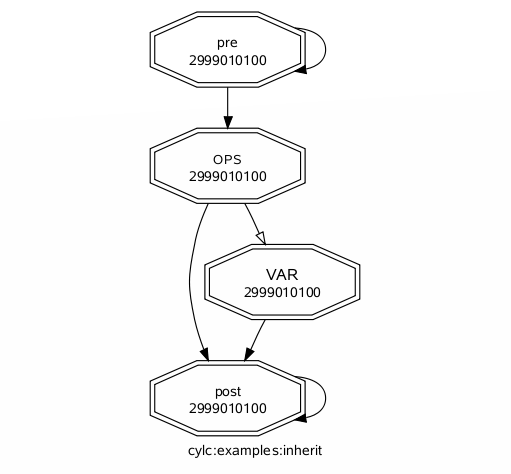
\includegraphics[width=\textwidth]{graphics/png/orig/inherit-2.png}
    \end{center}
\end{minipage}
\hfill
\begin{minipage}[t]{0.3\textwidth}
    \begin{center}
        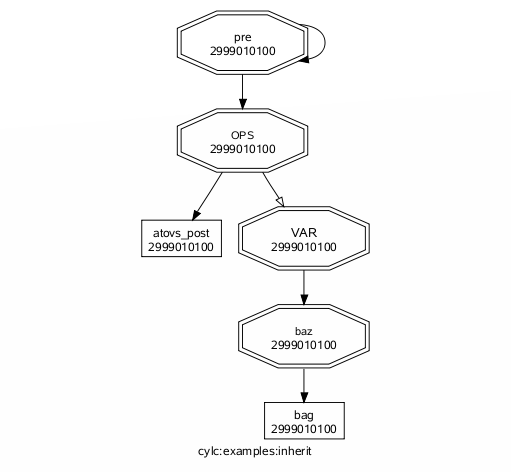
\includegraphics[width=\textwidth]{graphics/png/orig/inherit-3.png}
    \end{center}
\end{minipage}
\hfill
\begin{minipage}[t]{0.3\textwidth}
    \begin{center}
        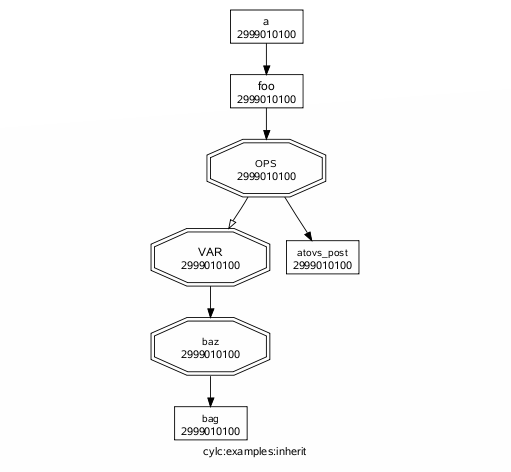
\includegraphics[width=\textwidth]{graphics/png/orig/inherit-4.png}
    \end{center}
\end{minipage}

\begin{minipage}[t]{0.3\textwidth}
    \begin{center}
        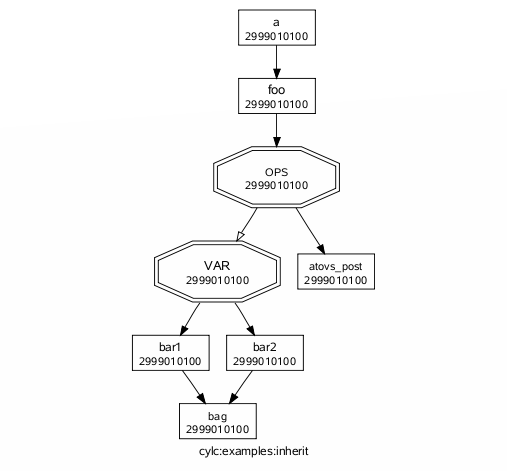
\includegraphics[width=\textwidth]{graphics/png/orig/inherit-5.png}
    \end{center}
\end{minipage}
\hfill
\begin{minipage}[t]{0.3\textwidth}
    \begin{center}
        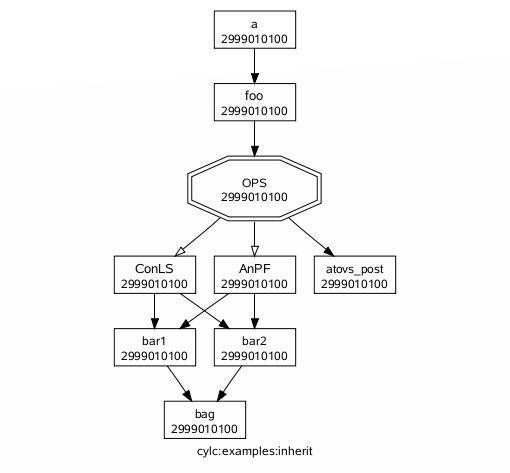
\includegraphics[width=\textwidth]{graphics/png/orig/inherit-6.png}
    \end{center}
\end{minipage}
\hfill
\begin{minipage}[t]{0.3\textwidth}
    \begin{center}
        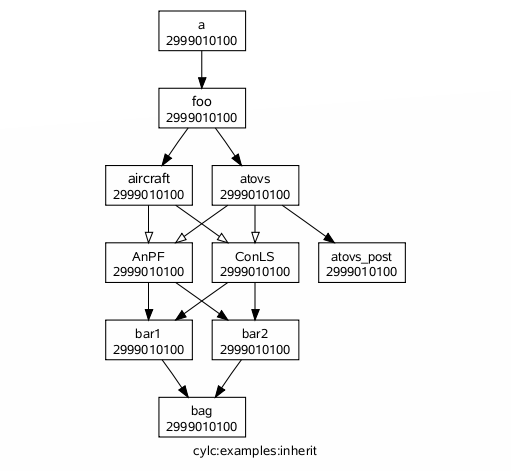
\includegraphics[width=\textwidth]{graphics/png/orig/inherit-7.png}
    \end{center}
\end{minipage}
\caption[{\em namespaces} example suite graphs]{\scriptsize Graphs of the {\em
namespaces} example suite showing various states of expansion of the
nested namespace family hierarchy, from all families collapsed (top
left) through to all expanded (bottom right). This can also be done by
right-clicking on tasks in the gcylc graph view.}
\label{fig-namespaces}
\end{figure}

\subsection{Parameterized Tasks}
\label{Parameterized Tasks}

Cylc can automatically generate tasks and dependencies by expanding
parameterized task names over lists of parameter values. Uses for this
include:
\begin{myitemize}
    \item generating an ensemble of similar model runs
    \item generating chains of tasks to process similar datasets
    \item replicating an entire workflow, or part thereof, over several runs
    \item splitting a long model run into smaller steps or ``chunks``
        (parameterized cycling)
\end{myitemize}

{\em Note that this can be done with Jinja2 loops too (Section~\ref{Jinja2})
    but parameterization is much cleaner (nested loops can seriously reduce
the clarity of a suite definition).}

\subsubsection{Parameter Expansion}

Parameter values can be lists of strings, or integer ranges (with inclusive bounds):
\begin{lstlisting}
[cylc]
    [[parameters]]
        obs = ship, buoy, plane
        run = 1..5  # 1, 2, 3, 4, 5
\end{lstlisting}
Then angle brackets denote use of these parameters throughout the suite
definition. For the values above, this parameterized name:
\begin{lstlisting}
    model<run>  # for run = 1..2
\end{lstlisting}
expands to these concrete task names:
\begin{lstlisting}
    model_run1, model_run2
\end{lstlisting}
and this parameterized name:
\begin{lstlisting}
    proc<obs>  # for obs = ship, buoy, plane
\end{lstlisting}
expands to these concrete task names:
\begin{lstlisting}
    proc_ship, proc_buoy, proc_plane
\end{lstlisting}
By default, to avoid any ambiguity, the parameter name appears in the expanded
task names for integer values, but not for string values. For example,
\lstinline=model_run1= for \lstinline@run = 1@, but \lstinline=proc_ship= for
\lstinline@obs = ship@. However, the default expansion templates can be
overridden if need be:
\begin{lstlisting}
[cylc]
    [[parameters]]
        obs = ship, buoy, plane
        run = 1..5
    [[parameter templates]]
        run = -R%(run)s  # Make foo<run> expand to foo-R1 etc.
\end{lstlisting}
(See~\ref{RefParameterTemplates} for more on the string template syntax.)

Any number of parameters can be used at once. This parameterization:
\begin{lstlisting}
    model<run,obs>  # for run = 1..2 and obs = ship, buoy, plane
\end{lstlisting}
expands to these tasks names:
\begin{lstlisting}
    model_run1_ship, model_run1_buoy, model_run1_plane,
    model_run2_ship, model_run2_buoy, model_run2_plane
\end{lstlisting}

Here's a simple but complete example suite:
\begin{lstlisting}
[cylc]
    [[parameters]]
        run = 1..2
[scheduling]
    [[dependencies]]
        graph = "prep => model<run>"
[runtime]
    [[model<run>]]
        # ...
\end{lstlisting}
The result, post parameter expansion, is this:
\begin{lstlisting}
[scheduling]
    [[dependencies]]
        graph = "prep => model_run1 & model_run2"
[runtime]
    [[model_run1]]
        # ...
    [[model_run2]]
        # ...
\end{lstlisting}

Here's a more complex graph using two parameters (\lstinline@[runtime]@ omitted):
\begin{lstlisting}
[cylc]
    [[parameters]]
        run = 1..2
        mem = cat, dog
[scheduling]
    [[dependencies]]
        graph = """prep => init<run> => model<run,mem> =>
                      post<run,mem> => wrap<run> => done"""
\end{lstlisting}
%which expands to:
%\begin{lstlisting}
%[scheduling]
%    [[dependencies]]
%        graph = """
%            prep => init_run1 => model_run1_cat => post_run1_cat => wrap_run1 => done
%                init_run1 => model_run1_dog => post_run2_dog => wrap_run1
%            prep => init_run2 => model_run2_cat => post_run2_cat => wrap_run2 => done
%                init_run2 => model_run2_dog => post_run2_dog => wrap_run2"""
%\end{lstlisting}
Figure~\ref{fig-params-1} shows the result as visualized by \lstinline=cylc graph=.
\begin{figure}
    \begin{center}
        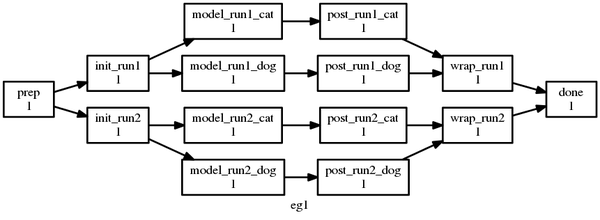
\includegraphics[width=10cm]{graphics/png/orig/params1.png}
    \end{center}
    \caption[Parameter expansion example.]{\scriptsize
     Parameter expansion example.}
    \label{fig-params-1}
\end{figure}

\paragraph{Zero-Padded Integer Values}

Integer parameter values are zero-padded according to the size of their
largest value, so \lstinline@foo<p>@ for \lstinline@p = 9..10@ expands to
\lstinline@foo_p09, foo_p10@.

To get thicker padding, prepend extra zeroes to the upper range value: 
\lstinline@foo<p>@ for \lstinline@p = 9..010@ expands to
\lstinline@foo_p009, foo_p010@.


\subsubsection{Passing Parameter Values To Tasks}

Parameter values are passed as environment variables to tasks generated by
parameter expansion. For the example above, task \lstinline=model_run2_ship=
would get the following environment variables:
\begin{lstlisting}
    $CYLC_TASK_PARAM_run  # value "2" etc.
    $CYLC_TASK_PARAM_obs  # value "ship" etc.
\end{lstlisting}
These variables allow tasks to determine which member of a parameterized
group they are, and so to vary their behaviour accordingly.


\subsubsection{Selecting Specific Parameter Values}

Specific parameter values can be singled out in the graph and under
\lstinline=[runtime]= with the notation \lstinline@<p=5>@ (for example).
Here's how to make a special task trigger off just the first of a
set of model runs:
\begin{lstlisting}
[cylc]
    [[parameters]]
        run = 1..5
[scheduling]
    [[dependencies]]
        graph = """model<run> => post_proc<run>  # general case
                   model<run=1> => check_first_run  # special case"""
[runtime]
    [[model<run>]]
        # config for all "model" runs...
    [[model<run=1>
        # special config (if any) for the first model run...
    #...
\end{lstlisting}

\subsubsection{Selecting Partial Parameter Ranges}

The parameter notation does not currently support partial range selection such
as \lstinline@foo<p=5..10>@, but you can achieve the same result by defining a
second parameter that covers the partial range and giving it the same expansion
template as the full-range parameter. For example:

\begin{lstlisting}
[cylc]
    [[parameters]]
        run = 1..10 # 01, 02, ..., 10
        runx = 1..03  # 01, 02, 03 (note `03' to get correct padding)
    [[parameter templates]]
        run = _R%(run)s
        runx = _R%(runx)s
[scheduling]
    [[dependencies]]
        graph = """model<run> => post<run>
                   model<runx> => checkx<runx>"""
[runtime]
    [[model<run>]]
        # ...
    #...
\end{lstlisting}


\subsubsection{Parameter Offsets In The Graph}

A negative offset notation \lstinline@<NAME-1>@ is interpreted as the
previous value in the ordered list of parameter values. For example, to split
a model run into multiple steps with each step depending on the previous one,
this graph:
\begin{lstlisting}
    graph = "model<run-1> => model<run>"  # for run = 1, 2, 3
\end{lstlisting}
expands to:
\begin{lstlisting}
    graph = """model_run1 => model_run2
               model_run2 => model_run3"""
# or equivalently:
    graph = "model_run1 => model_run2 => model_run3"
\end{lstlisting}
And this graph:
\begin{lstlisting}
    graph = "proc<size-1> => proc<size>"  # for size = small, big, huge
\end{lstlisting}
expands to:
\begin{lstlisting}
    graph = """proc_small => proc_big
               proc_big => proc_huge"""
# or equivalently:
    graph = "proc_small => proc_big => proc_huge"
\end{lstlisting}

\subsubsection{Task Families And Parameterization}

Task family members can be generated by parameter expansion:
\begin{lstlisting}
[runtime]
    [[FAM]]
    [[member<r>]]
        inherit = FAM
# Result: family FAM contains member_r1, member_r2, etc.
\end{lstlisting}

Family names can be parameterized too, just like task names:
\begin{lstlisting}
[runtime]
    [[RUN<r>]]
    [[model<r>]]
        inherit = RUN<r>
    [[post_proc<r>]]
        inherit = RUN<r>
# Result: family RUN_r1 contains model_r1 and post_proc_r1,
#         family RUN_r2 contains model_r2 and post_proc_r1, etc.
\end{lstlisting}

As described in Section~\ref{FamilyTriggers} family names can be used to
trigger all members at once:
\begin{lstlisting}
    graph = "foo => FAMILY"
\end{lstlisting}
or to trigger off all members:
\begin{lstlisting}
    graph = "FAMILY:succeed-all => bar"
\end{lstlisting}
or to trigger off any members:
\begin{lstlisting}
    graph = "FAMILY:succeed-any => bar"
\end{lstlisting}

If the members of \lstinline=FAMILY= were generated with parameters, you can
also trigger them all at once with parameter notation:
\begin{lstlisting}
    graph = "foo => member<m>"
\end{lstlisting}
Similarly, to trigger off all members:
\begin{lstlisting}
    graph = "member<m> => bar"
    # (member<m>:fail etc., for other trigger types)
\end{lstlisting}

Family names are still needed in the graph, however, to succinctly express
``succeed-any'' triggering semantics, and all-to-all or any-to-all triggering:
\begin{lstlisting}
    graph = "FAM1:succeed-any => FAM2"
\end{lstlisting}
(Direct all-to-all and any-to-all family triggering is not recommended for
efficiency reasons though - see Section~\ref{EfficientInterFamilyTriggering}).

For family {\em member-to-member} triggering use parameterized members.
For example, if family \lstinline=OBS_GET= has members \lstinline=get<obs>= and
family \lstinline=OBS_PROC= has members \lstinline=proc<obs>= then this graph:
\begin{lstlisting}
    graph = "get<obs> => proc<obs>"  # for obs = ship, buoy, plane
\end{lstlisting}
expands to:
\begin{lstlisting}
    get_ship => proc_ship
    get_buoy => proc_buoy
    get_plane => proc_plane
\end{lstlisting}

\subsubsection{Parameterized Cycling}
\label{Parameterized Cycling}

Parameterized cycling is described and contrasted with iterative cycling in
Section~\ref{Ways Of Cycling}. In iterative cycling (which is recommended in
most cases) each instance of a cycled job is run by the same logical task at
different cycle points, and the scheduler extends the workflow to future cycle
points as the suite runs, potentially indefinitely.  In parameterized cycling,
parameter expansion (or Jinja2 loops) is used to generate the entire workflow
(every task instance from start to finish) at start-up. Each instance of a
cycled job is run by a different logical task with a different task name, and
the only ``cycling'' that occurs in the scheduler is during the workflow
definition phase at start-up.

Here's an iterative cycling workflow of two-monthly model runs for one year,
with previous-instance model dependence (e.g.\ for model restart files):
\lstset{language=suiterc}
\begin{lstlisting}
[scheduling]
    initial cycle point = 2020-01
    final cycle point = 2020-12
    [[dependencies]]
        [[[R1]]]  # Run once, at the initial point.
            graph = "prep => model"
        [[[P2M]]]  # Run at 2-month intervals between the initial and final points.
            graph = "model[-P2M] => model => post_proc & archive"
[runtime]
    [[model]]
        script = "run-model $CYLC_TASK_CYCLE_POINT"
\end{lstlisting}

And here's how to do the same thing with parameterized tasks:
\lstset{language=suiterc}
\begin{lstlisting}
[cylc]
    [[parameters]]
        chunk = 1..6
[scheduling]
    [[dependencies]]
        graph = """prep => model<chunk=1>
                     model<chunk-1> => model<chunk> =>
                       post_proc<chunk> & archive<chunk>"""
[runtime]
    [[model<chunk>]]
        script = """
# Compute start date from chunk index and interval, then run the model.
INITIAL_POINT=2020-01
INTERVAL_MONTHS=2
OFFSET_MONTHS=(( (CYLC_TASK_PARAM_chunk - 1)*INTERVAL_MONTHS ))
OFFSET=P${OFFSET_MONTHS}M  # e.g. P4M for chunk=3
run-model $(cylc cyclepoint --offset=$OFFSET $INITIAL_POINT)"""
\end{lstlisting}

The two workflows are shown together in Figure~\ref{fig-eg2}. They both achieve
the same result, and special tasks at the start or end, or anywhere in between,
can easily be added in both cases. But note that parameterized version has
several disadvantages: it must be finite in extent and not too large; the
date-time arithmetic has to be done manually; and the full extent of the workflow
will be visible at all times as the suite runs - because it does not have
``cycle points''.

\begin{figure}
    \begin{center}
        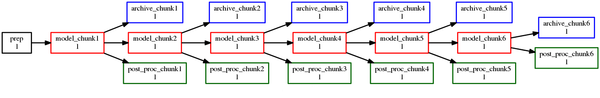
\includegraphics[width=16cm]{graphics/png/orig/eg2-static.png}
    \end{center}
    \begin{center}
        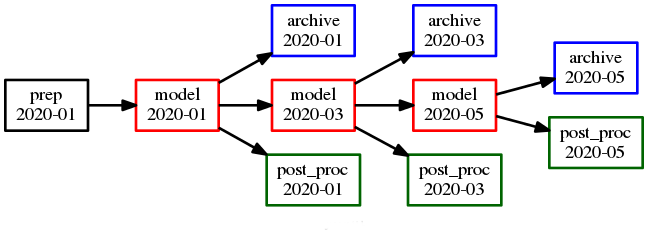
\includegraphics[width=10cm]{graphics/png/orig/eg2-dynamic.png}
    \end{center}
    \caption[Parameterized (top) and iterative cycling (bottom) versions of the
        same workflow.]{\scriptsize parameterized and iterative cycling versions
            of the same workflow. The first three cycle points are shown in the
            iterative case (the parameterized case does not have ``cycle
        points'').}
    \label{fig-eg2}
\end{figure}

Here's a yearly-cycling suite with four parameterized chunks in each cycle
point:
\begin{lstlisting}
[cylc]
    [[parameters]]
        chunk = 1..4
[scheduling]
    initial cycle point = 2020-01
    [[dependencies]]
        [[[P1Y]]]
            graph = """model<chunk-1> => model<chunk>
                    model<chunk=4>[-P1Y] => model<chunk=1>"""
\end{lstlisting}
Note the inter-cycle trigger that connects the first chunk in each cycle point
to the last chunk in the previous cycle point. Of course it would be simpler
to just use 3-monthly iterative cycling:
\begin{lstlisting}
[scheduling]
    initial cycle point = 2020-01
    [[dependencies]]
        [[[P3M]]]
            graph = "model[-P3M] => model"
\end{lstlisting}

A possible use-case for mixed iterative and parameterized cycling: consider a
portable date-time cycling workflow of model jobs that can each take too long
to run, or not, depending on the host platform.  This could be handled without
changing the (iterative) cycling structure of the suite, by splitting the run
(at each cycle point) into a variable number of shorter steps, using more steps
on less powerful hosts.

\paragraph{Cycle Point And Parameter Offsets At Start-Up}

In iterative cycling, cylc ignores anything earlier than the suite initial
cycle point. So this graph:
\begin{lstlisting}
    graph = "model[-P1D] => model"
\end{lstlisting}
simplifies at the initial cycle point to:
\begin{lstlisting}
    graph = "model"
\end{lstlisting}

Similarly, parameter offsets are ignored if they extend beyond the start of the
parameter value list. So this graph:
\begin{lstlisting}
    graph = "model<chunk-1> => model<chunk>"
\end{lstlisting}
simplifies for \lstinline@chunk=1@ to this:
\begin{lstlisting}
    graph = "model_chunk1"
\end{lstlisting}

Note however that the initial cut-off applies to every parameter list, but only
to cycle point sequences that start at the suite initial cycle point. Therefore
it may be somewhat easier to use parameterized cycling if you need multiple
date-time sequences {\em with different start points} in the same suite. We
plan to allow this sequence-start simplification for any date-time sequence in
the future, not just at the suite initial point, but it needs to be optional
because delayed-start cycling tasks sometimes need to trigger off earlier
cycling tasks.

\subsection{Jinja2}
\label{Jinja2}

{\em This section needs to be revised - the Parameterized Task feature
    introduced in cylc-6.11.0 (see Section~\ref{Parameterized Tasks}) provides
    a cleaner way to auto-generate tasks without coding messy Jinja2 loops.}

Cylc has built in support for the Jinja2 template processor in suite
definitions. Jinja2 variables, mathematical expressions, loop control
structures, conditional logic, etc., are automatically processed to
generate the final suite definition seen by cylc.

The need for Jinja2 processing must be declared with a hash-bang
comment as the first line of the suite.rc file:
\begin{lstlisting}
#!jinja2
# ...
\end{lstlisting}

Potential uses for this include automatic generation of repeated groups
of similar tasks and dependencies, and inclusion or exclusion of entire
suite sections according to the value of a single flag. Consider a
large complicated operational suite and several related parallel test
suites with slightly different task content and structure (the parallel
suites, for instance, might take certain large input files from the
operation or the archive rather than downloading them again) - these can
now be maintained as a single master suite definition that reconfigures
itself according to the value of a flag variable indicating the intended use.

Template processing is the first thing done on parsing a suite
definition so Jinja2 expressions can appear anywhere in the file (inside
strings and namespace headings, for example).

Jinja2 is well documented at \url{http://jinja.pocoo.org/docs}, so here
we just provide an example suite that uses it. The meaning of the
embedded Jinja2 code should be reasonably self-evident to anyone familiar
with standard programming techniques.

\begin{figure}
    \begin{center}
        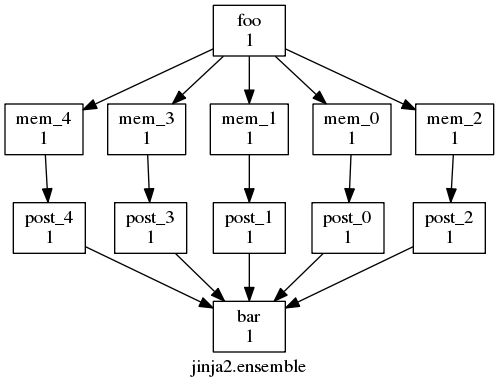
\includegraphics[width=10cm]{graphics/png/orig/jinja2-ensemble-graph.png}
    \end{center}
    \caption[The Jinja2 ensemble example suite graph.]{\scriptsize
    The Jinja2 ensemble example suite graph.}
    \label{fig-jinja2-ensemble}
\end{figure}

The \lstinline=jinja2.ensemble= example, graphed in
Figure~\ref{fig-jinja2-ensemble}, shows an ensemble of similar tasks
generated using Jinja2:
\lstset{language=suiterc}
\begin{lstlisting}
#!jinja2

[scheduling]
    [[dependencies]]
        graph = """{# generate ensemble dependencies #}
            
               foo => mem_{{ I }} => post_{{ I }} => bar
            """
\end{lstlisting}
Here is the generated suite definition, after Jinja2 processing:
\lstset{language=suiterc}
\begin{lstlisting}
#!jinja2
[scheduling]
    [[dependencies]]
        graph = """
          foo => mem_0 => post_0 => bar
          foo => mem_1 => post_1 => bar
          foo => mem_2 => post_2 => bar
          foo => mem_3 => post_3 => bar
          foo => mem_4 => post_4 => bar
                """
\end{lstlisting}

And finally, the \lstinline=jinja2.cities= example uses variables,
includes or excludes special cleanup tasks according to the value of a
logical flag, and it automatically generates all dependencies and family
relationships for a group of tasks that is repeated for each city in the
suite. To add a new city and associated tasks and dependencies simply
add the city name to list at the top of the file. The suite is graphed,
with the New York City task family expanded, in
Figure~\ref{fig-jinja2-cities}.

\lstset{language=suiterc}
\lstinputlisting{../examples/jinja2/cities/suite.rc}
\lstset{language=transcript}

\begin{figure}
    \begin{center}
        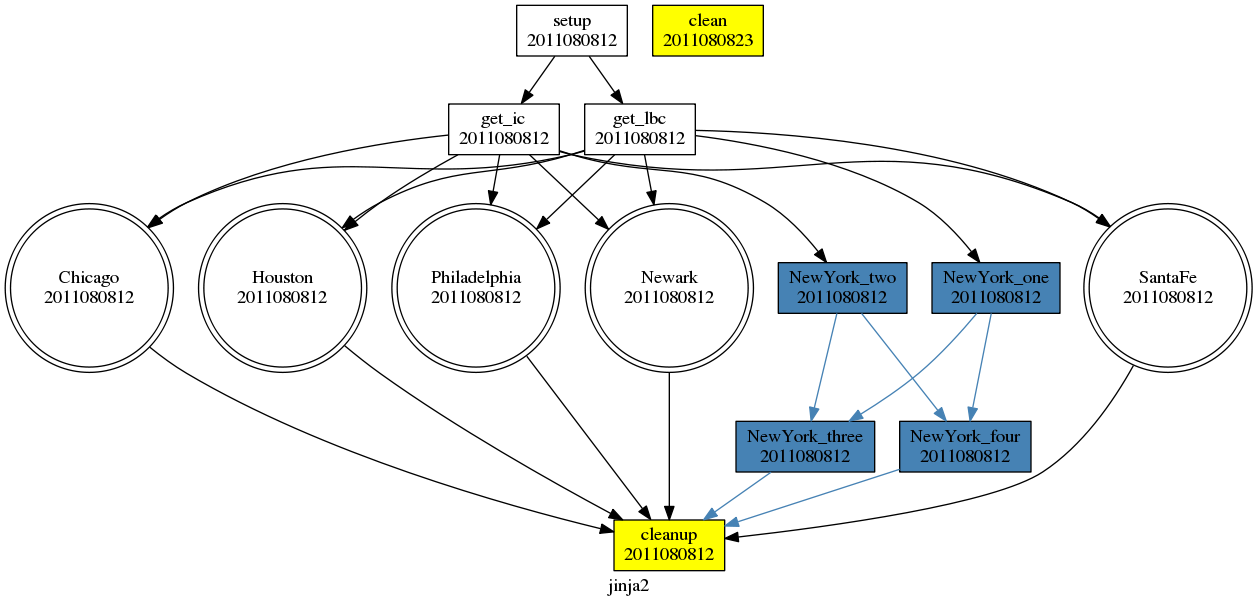
\includegraphics[width=16cm]{graphics/png/orig/jinja2-suite-graph.png}
    \end{center}
    \caption[Jinja2 cities example suite graph.]{\scriptsize
    The Jinja2 cities example suite graph, with the
    New York City task family expanded.}
    \label{fig-jinja2-cities}
\end{figure}

\subsubsection{Accessing Environment Variables With Jinja2}

This functionality is not provided by Jinja2 by default, but cylc
automatically imports the user environment to the template in a
dictionary structure called {\em environ}. A usage example:
\begin{lstlisting}
#!Jinja2
#...
[runtime]
    [[root]]
        [[[environment]]]
            SUITE_OWNER_HOME_DIR_ON_SUITE_HOST = {{environ['HOME']}}
\end{lstlisting}
This example is emphasizes that {\em the environment is read on the suite
host at the time the suite definition is parsed} - it is not, for
instance, read at task run time on the task host.

\subsubsection{Custom Jinja2 Filters}
\label{CustomJinja2Filters}

Jinja2 variable values can be modified by ``filters'', using pipe
notation. For example, the built-in \lstinline=trim= filter strips
leading and trailing white space from a string:
\lstset{language=suiterc}
\begin{lstlisting}

{{ MyString | trim() }}  # "dog"
\end{lstlisting}
(See official Jinja2 documentation for available built-in filters.)

Cylc also supports custom Jinja2 filters. A custom filter is a
single Python function in a source file with the same name as the
function (plus ``.py'' extension) and stored in one of the following
locations:
\begin{myitemize}
    \item \lstinline=$CYLC_DIR/lib/Jinja2Filters/=
    \item \lstinline=[suite definition directory]/Jinja2Filters/=
    \item \lstinline=$HOME/.cylc/Jinja2Filters/=
\end{myitemize}

In the filter function argument list, the first argument is the variable
value to be ``filtered'', and subsequent arguments can be whatever is
needed. Currently there is one custom filter called ``pad'' in the
central cylc Jinja2 filter directory, for padding string values to some
constant length with a fill character - useful for generating task names
and related values in ensemble suites:

\lstset{language=suiterc}
\begin{lstlisting}
  # 0, 1, ..., 99
    
    A_{{j}}          # A_00, A_01, ..., A_99

\end{lstlisting}

\subsubsection{Associative Arrays In Jinja2}

Associative arrays ({\em dicts} in Python) can be very useful.
Here's an example, from \\*
\lstinline=$CYLC_DIR/examples/jinja2/dict=:

\lstset{language=suiterc}
\begin{lstlisting}
#!Jinja2



[scheduling]
    [[dependencies]]
        graph = OBS
[runtime]
    [[OBS]]
        [[[job]]]
            batch system = pbs
    
    [[ {{i}} ]]
        inherit = OBS
        [[[directives]]]
             -I = {{ resource[i] }}
     
 \end{lstlisting}

Here's the result:
\lstset{language=transcript}
\begin{lstlisting}
shell$ cylc get-suite-config -i [runtime][airs]directives SUITE
-I = ncpus=9
\end{lstlisting}

\subsubsection{Jinja2 Default Values And Template Inputs}

The values of Jinja2 variables can be passed in from the cylc command
line rather than hardwired in the suite definition.
Here's an example, from \\*
\lstinline=$CYLC_DIR/examples/jinja2/defaults=:

\lstset{language=suiterc}
\begin{lstlisting}
#!Jinja2

title = "Jinja2 example: use of defaults and external input"

description = """
The template variable FIRST_TASK must be given on the cylc command line
using --set or --set-file=FILE; two other variables, LAST_TASK and
N_MEMBERS can be set similarly, but if not they have default values."""




{# input of FIRST_TASK is required - no default #}

[scheduling]
    initial cycle point = 20100808T00
    final cycle point   = 20100816T00
    [[dependencies]]
        [[[0]]]
            graph = """{{ FIRST_TASK }} => ENS
                 ENS:succeed-all => {{ LAST_TASK }}"""
[runtime]
    [[ENS]]

    [[ mem_{{ I }} ]]
        inherit = ENS

\end{lstlisting}

Here's the result:

\lstset{language=transcript}
\begin{lstlisting}
shell$ cylc list SUITE
Jinja2 Template Error
'FIRST_TASK' is undefined
cylc-list foo  failed:  1

shell$ cylc list --set FIRST_TASK=bob foo
bob
baz
mem_2
mem_1
mem_0

shell$ cylc list --set FIRST_TASK=bob --set LAST_TASK=alice foo
bob
alice
mem_2
mem_1
mem_0

shell$ cylc list --set FIRST_TASK=bob --set N_MEMBERS=10 foo
mem_9
mem_8
mem_7
mem_6
mem_5
mem_4
mem_3
mem_2
mem_1
mem_0
baz
bob
\end{lstlisting}

\lstset{language=suiterc}
Note also that
\lstinline@cylc view --set FIRST_TASK=bob --jinja2 SUITE@ will show the
suite with the Jinja2 variables as set.

{\em Note:} suites started with template variables set on the command
line will {\em restart} with the same settings. However, you can set
them again on the \lstinline=cylc restart= command line if they need to
be overridden.


\subsection{Omitting Tasks At Runtime}

It is sometimes convenient to omit certain tasks from the suite at
runtime without actually deleting their definitions from the suite.

Defining [runtime] properties for tasks that do not appear in the suite
graph results in verbose-mode validation warnings that the tasks are
disabled. They cannot be used because the suite graph is what defines
their dependencies and valid cycle points. Nevertheless, it is legal to
leave these orphaned runtime sections in the suite definition because it
allows you to temporarily remove tasks from the suite by simply
commenting them out of the graph.

To omit a task from the suite at runtime but still leave it fully
defined and available for use (by insertion or \lstinline=cylc submit=)
use one or both of [scheduling][[special task]] lists, {\em include at
start-up} or {\em exclude at start-up} (documented in~\ref{IASU}
and~\ref{EASU}). Then the graph still defines the
validity of the tasks and their dependencies, but they are not actually
loaded into the suite at start-up. Other tasks that depend on the
omitted ones, if any, will have to wait on their insertion at a later
time or otherwise be triggered manually.

Finally, with Jinja2 (\ref{Jinja2}) you can radically alter
suite structure by including or excluding tasks from the [scheduling]
and [runtime] sections according to the value of a single logical flag
defined at the top of the suite.
\subsection{Naked Dummy Tasks And Strict Validation}

A {\em naked dummy task} appears in the suite graph but has no
explicit runtime configuration section. Such tasks automatically
inherit the default ``dummy task'' configuration from the root
namespace. This is very useful because it allows functional suites to
be mocked up quickly for test and demonstration purposes by simply
defining the graph. It is somewhat dangerous, however, because there
is no way to distinguish an intentional naked dummy task from one
generated by typographic error: misspelling a task name in the graph
results in a new naked dummy task replacing the intended task in the
affected trigger expression; and misspelling a task name in a runtime
section heading results in the intended task becoming a dummy task
itself (by divorcing it from its intended runtime config section).

To avoid this problem any dummy task used in a real suite should not be
naked - i.e.\ it should have an explicit entry in under the runtime
section of the suite definition, even if the section is empty. This
results in exactly the same dummy task behaviour, via implicit
inheritance from root, but it allows use of
\lstinline=cylc validate --strict=
to catch errors in task names by failing the suite if any naked dummy
tasks are detected.

\section{Task Implementation}
\label{TaskImplementation}

Existing scripts or executables can be used as cylc tasks without any
modification so long as they return standard exit status on success or
failure, and do not internally spawn detaching processes
(see~\ref{DetachingJobs}).

\subsection{Inlined Tasks}

Simple tasks can be entirely implemented within the suite.rc file,
as the task {\em script} items can be multi-line strings.

\subsection{Returning Proper Error Status}

Tasks should abort with non-zero exit status if a fatal error occurs
(this is just good coding practice anyway). This allows cylc's task
job scripts to automatically trap errors and send
\lstinline=cylc task message "failed"= back to the suite. The shell
\lstinline=set -e= option can be used in lieu of explicit error
checks for every command:
\lstset{language=bash}
\begin{lstlisting}
#!/bin/bash
set -e  # abort on error
mkdir /illegal/dir  # this will abort the script with error status
\end{lstlisting}


\subsection{Other Task Messages}

General (non-output) messages can also be sent to report progress,
warnings, and so on, e.g.:
\lstset{language=bash}
\begin{lstlisting}
#!/bin/bash
# a warning message (this will be logged by the suite):
cylc task message -p WARNING "oops, something's fishy here"
# information (this will also be logged by the suite):
cylc task message "Hello from task foo"
\end{lstlisting}

Explanatory messages can be sent before aborting on error:
\lstset{language=bash}
\begin{lstlisting}
#!/bin/bash
set -e  # abort on error
if ! mkdir /illegal/dir; then
    # (use inline error checking to avoid triggering the above 'set -e')
    cylc task message -p CRITICAL "Failed to create directory /illegal/dir"
    exit 1 # now abort non-zero exit status to trigger the task failed message
fi
\end{lstlisting}
Or equivalently, with different syntax:
\lstset{language=bash}
\begin{lstlisting}
#!/bin/bash
set -e
mkdir /illegal/dir || {  # inline error checking using OR operator
    cylc task message -p CRITICAL "Failed to create directory /illegal/dir"
    exit 1
}
\end{lstlisting}
But not this:
\lstset{language=bash}
\begin{lstlisting}
#!/bin/bash
set -e
mkdir /illegal/dir  # aborted via 'set -e'
if [[ $? != 0 ]]; then  # so this will never be reached.
    cylc task message -p CRITICAL "Failed to create directory /illegal/dir"
    exit 1
fi
\end{lstlisting}
If critical errors are not reported in this way task failures will still
be detected and logged by the suite daemon, but you may have to examine task
logs to determine what the problem was.

\subsection{Avoid Detaching Processes}
\label{DetachingJobs}

\lstset{language=transcript}
If a task script starts background sub-processes and does not wait on them, or
internally submits jobs to a batch scheduler and then exits immediately, the
detached processes will not be visible to cylc and the task will appear to
finish when the top-level script finishes. You will need to modify scripts
like this to make them execute all sub-processes in the foreground (or use the
shell \lstinline=wait= command to wait on them before exiting) and to prevent
job submission commands from returning before the job completes (e.g.\
\lstinline=llsubmit -s= for Loadleveler,
\lstinline=qsub -sync yes= for Sun Grid Engine, and
\lstinline@qsub -W block=true@ for PBS).

If this is not possible - perhaps you don't have control over the script
or can't work out how to fix it - one alternative approach is to use another
task to repeatedly poll for the results of the detached processes:
\begin{lstlisting}
[scheduling]
    [[dependencies]]
        graph = "model => checker => post-proc"
[runtime]
    [[model]]
        # Uh-oh, this script does an internal job submission to run model.exe:
        script = "run-model.sh"
    [[checker]]
        # Fail and retry every minute (for 10 tries at the most) if the model's
        # job.done indicator file does not exist yet.
        retry delays = 10 * PT1M
        script = "[[ ! -f $RUN_DIR/job.done ]] && exit 1"
\end{lstlisting}

\section{Task Job Submission and Management}
\label{TaskJobSubmission}

For the requirements a command, script, or program, must fulfill in order
to function as a cylc task, see~\ref{TaskImplementation}.
This section explains how tasks are submitted by the suite daemon when they are
ready to run, and how to define new task job submission methods.

\subsection{Task Job Scripts}
\label{JobScripts}

When a task is ready cylc generates a {\em task job script} that encapsulates
the runtime settings (environment and scripting) defined for it in the suite.rc
file. The job script is submitted to run by the {\em job submission method}
chosen for the task. Different tasks can have different job submission methods.
Like other runtime properties, you can set a suite default job submission
method and override it for specific tasks or families:
\lstset{language=suiterc}
\begin{lstlisting}
[runtime]
   [[root]] # suite defaults
        [[[job]]]
            batch system = loadleveler
   [[foo]] # just task foo
        [[[job]]]
            batch system = at
\end{lstlisting}

As shown in the Tutorial (\ref{RunningSuitesCLI}) job scripts are
saved to the suite run directory; the commands used to submit them are
printed to stdout by cylc in debug mode; and they can be printed with the
\lstinline=cylc cat-log= command or new ones generated and printed with the
\lstinline=cylc jobscript= command. Take a look at one to see exactly
how cylc wraps and runs your tasks.

\subsection{Supported Job Submission Methods}
\label{AvailableMethods}

Cylc supports a number of commonly used job submission methods.
See~\ref{CustomJobSubmissionMethods} for how to add new job
submission methods.

\subsubsection{background}

Runs tasks as Unix background processes.

If an execution time limit is specified for a task, its job will be wrapped
by the \lstinline=timeout= command.

\subsubsection{at}

Submits tasks to the rudimentary Unix \lstinline=at= scheduler. The
\lstinline=atd= daemon must be running.

If an execution time limit is specified for a task, its job will be wrapped
by the \lstinline=timeout= command.

\subsubsection{loadleveler}

Submits tasks to loadleveler by the \lstinline=llsubmit= command.
Loadleveler directives can be provided in the suite.rc file:

\lstset{language=suiterc}
\begin{lstlisting}
[runtime]
    [[my_task]]
        [[[job]]]
            batch system = loadleveler
            execution time limit = PT10M
        [[[directives]]]
            foo = bar
            baz = qux
\end{lstlisting}
These are written to the top of the task job script like this:
\lstset{language=bash}
\begin{lstlisting}
#!/bin/bash
# DIRECTIVES
# @ foo = bar
# @ baz = qux
# @ wall_clock_limit = 660,600
# @ queue
\end{lstlisting}

If restart=yes is specified as a directive for loadleveler, the job will
automatically trap SIGUSR1, which loadleveler may use to preempt the job. On
trapping SIGUSR1, the job will inform the suite that it has been vacated by
loadleveler. This will put it back to the submitted state, until it starts
running again.

If \lstinline=execution time limit= is specified, it is used to generate the
\lstinline=wall_clock_limit= directive. The setting is assumed to be the soft
limit. The hard limit will be set by adding an extra minute to the soft limit.
Do not specify the \lstinline=wall_clock_limit= directive explicitly if
\lstinline=execution time limit= is specified. Otherwise, the execution time
limit known by the suite may be out of sync with what is submitted to the batch
system.

\subsubsection{lsf}

Submits tasks to IBM Platform LSF by the \lstinline=bsub= command.
LSF directives can be provided in the suite.rc file:

\lstset{language=suiterc}
\begin{lstlisting}
[runtime]
    [[my_task]]
        [[[job]]]
            batch system = lsf
            execution time limit = PT10M
        [[[directives]]]
            -q = foo
\end{lstlisting}
These are written to the top of the task job script like this:
\lstset{language=bash}
\begin{lstlisting}
#!/bin/bash
# DIRECTIVES
#BSUB -q = foo
#BSUB -W = 10
\end{lstlisting}

If \lstinline=execution time limit= is specified, it is used to generate the
\lstinline=-W= directive. Do not specify the \lstinline=-W= directive
explicitly if \lstinline=execution time limit= is specified. Otherwise, the
execution time limit known by the suite may be out of sync with what is
submitted to the batch system.

\subsubsection{pbs}

Submits tasks to PBS (or Torque) by the \lstinline=qsub= command. PBS
directives can be provided in the suite.rc file:
\lstset{language=suiterc}
\begin{lstlisting}
[runtime]
    [[my_task]]
        [[[job]]]
            batch system = pbs
            execution time limit = PT1M
        [[[directives]]]
            -V =
            -q = foo
            -l nodes = 1
\end{lstlisting}
These are written to the top of the task job script like this:
\lstset{language=bash}
\begin{lstlisting}
#!/bin/bash
# DIRECTIVES
#PBS -V
#PBS -q foo
#PBS -l nodes=1
#PBS -l walltime=60
\end{lstlisting}

If \lstinline=execution time limit= is specified, it is used to generate the
\lstinline=-l walltime= directive. Do not specify the \lstinline=-l walltime=
directive explicitly if \lstinline=execution time limit= is specified.
Otherwise, the execution time limit known by the suite may be out of sync with
what is submitted to the batch system.

\subsubsection{moab}

Submits tasks to the Moab workload manager by the \lstinline=msub= command.
Moab directives can be provided in the suite.rc file; the syntax is very
similar to PBS:
\lstset{language=suiterc}
\begin{lstlisting}
[runtime]
    [[my_task]]
        [[[job]]]
            batch system = moab
            execution time limit = PT1M
        [[[directives]]]
            -V =
            -q = foo
            -l nodes = 1
\end{lstlisting}
These are written to the top of the task job script like this:
\lstset{language=bash}
\begin{lstlisting}
#!/bin/bash
# DIRECTIVES
#PBS -V
#PBS -q foo
#PBS -l nodes=1
#PBS -l walltime=60
\end{lstlisting}
(Moab understands \lstinline=#PBS= directives).

If \lstinline=execution time limit= is specified, it is used to generate the
\lstinline=-l walltime= directive. Do not specify the \lstinline=-l walltime=
directive explicitly if \lstinline=execution time limit= is specified.
Otherwise, the execution time limit known by the suite may be out of sync with
what is submitted to the batch system.

\subsubsection{sge}

Submits tasks to Sun/Oracle Grid Engine by the \lstinline=qsub= command.
SGE directives can be provided in the suite.rc file:
\lstset{language=suiterc}
\begin{lstlisting}
[runtime]
    [[my_task]]
        [[[job]]]
            batch system = sge
            execution time limit = P1D
        [[[directives]]]
            -cwd =
            -q = foo
            -l h_data = 1024M
            -l h_rt = 24:00:00
\end{lstlisting}
These are written to the top of the task job script like this:
\lstset{language=bash}
\begin{lstlisting}
#!/bin/bash
# DIRECTIVES
#$ -cwd
#$ -q foo
#$ -l h_data=1024M
#$ -l h_rt=24:00:00
\end{lstlisting}

If \lstinline=execution time limit= is specified, it is used to generate the
\lstinline=-l h_rt= directive. Do not specify the \lstinline=-l h_rt=
directive explicitly if \lstinline=execution time limit= is specified.
Otherwise, the execution time limit known by the suite may be out of sync with
what is submitted to the batch system.

\subsubsection{slurm}

Submits tasks to Simple Linux Utility for Resource Management by the
\lstinline=sbatch= command. SLURM directives can be provided in the
suite.rc file (note that since not all SLURM commands have a short form,
cylc requires the long form directives):
\lstset{language=suiterc}
\begin{lstlisting}
[runtime]
    [[my_task]]
        [[[job]]]
            batch system = slurm
            execution time limit = PT1H
        [[[directives]]]
            --nodes = 5
            --account = QXZ5W2
\end{lstlisting}
These are written to the top of the task job script like this:
\lstset{language=bash}
\begin{lstlisting}
#!/bin/bash
#SBATCH --nodes=5
#SBATCH --time=60:00
#SBATCH --account=QXZ5W2
\end{lstlisting}

If \lstinline=execution time limit= is specified, it is used to generate the
\lstinline=--time= directive. Do not specify the \lstinline=--time=
directive explicitly if \lstinline=execution time limit= is specified.
Otherwise, the execution time limit known by the suite may be out of sync with
what is submitted to the batch system.

\subsubsection{Default Directives Provided}

For job submission methods that use job file directives (PBS, Loadleveler,
etc.) default directives are provided to set the job name, stdout and stderr
file paths, and the execution time limit (if specified).

Cylc constructs the job name string using a combination of the task ID and the
suite name. PBS fails a job submit if the job name in \lstinline=-N name= is
too long. For version 12 or below, this is 15 characters. For version 13, this
is 236 characters. The default setting will truncate the job name string to 15
characters. If you have PBS 13 at your site, you should modify your site's
global configuration file to allow the job name to be longer. (See also
Section~\ref{JobNameLengthMaximum}.) For example:

\begin{lstlisting}
[hosts]
    [[myhpc*]]
        [[[batch systems]]]
            [[[[pbs]]]]
                # PBS 13
                job name length maximum = 236
\end{lstlisting}

\subsubsection{Directives Section Quirks (PBS, SGE, ...) }

As shown in the example above, to get a naked option flag such as
\lstinline=-V= in PBS or \lstinline=-cwd= in SGE you must give a
null string as the directive value in the suite.rc file.

\subsection{Task stdout And stderr Logs}
\label{WhitherStdoutAndStderr}

When a task is ready to run cylc generates a filename root to be used
for the task job script and log files. The filename containing the task
name, cycle point, and a submit number that increments if the same task is
re-triggered multiple times:

\lstset{language=bash}
\begin{lstlisting}
# task job script:
~/cylc-run/tut.oneoff.basic/log/job/1/hello/01/job
# task stdout:
~/cylc-run/tut.oneoff.basic/log/job/1/hello/01/job.out
# task stderr:
~/cylc-run/tut.oneoff.basic/log/job/1/hello/01/job.err
\end{lstlisting}

How the stdout and stderr streams are directed into these files depends
on the job submission method. The \lstinline=background= method just uses
appropriate output redirection on the command line, as shown above. The
\lstinline=loadleveler= method writes appropriate directives to the job
script that is submitted to loadleveler.

Cylc obviously has no control over the stdout and stderr output from
tasks that do their own internal output management (e.g.\ tasks
that submit internal jobs and direct the associated output to other
files). For less internally complex tasks, however, the files referred
to here will be complete task job logs.

Some job submission methods, such as \lstinline=pbs=, redirect a job's stdout
and stderr streams to a separate cache area while the job is running. The
contents are only copied to the normal locations when the job completes. This
means that \lstinline=cylc cat-log= or the gcylc GUI will be unable to find the
job's stdout and stderr streams while the job is running. Some sites with these
job submission methods are known to provide commands for viewing and/or
tail-follow a job's stdout and stderr streams that are redirected to these
cache areas. If this is the case at your site, you can configure cylc to make
use of the provided commands by adding some settings to the global site/user
config. E.g.:

\begin{lstlisting}
[hosts]
    [[HOST]]  # <= replace this with a real host name
        [[[batch systems]]]
            [[[[pbs]]]]
                err tailer = qcat -f -e \%(job_id)s
                out tailer = qcat -f -o \%(job_id)s
                err viewer = qcat -e \%(job_id)s
                out viewer = qcat -o \%(job_id)s
\end{lstlisting}

\subsection{Overriding The Job Submission Command}
\label{CommandTemplate}

\lstset{language=suiterc}
To change the form of the actual command used to submit a job you do not
need to define a new job submission method; just override the
\lstinline=command template= in the relevant job submission sections of
your suite.rc file:
\begin{lstlisting}
[runtime]
    [[root]]
        [[[job]]]
            batch system = loadleveler
            # Use '-s' to stop llsubmit returning
            # until all job steps have completed:
            batch submit command template = llsubmit -s %(job)s
\end{lstlisting}
As explained in~\ref{SuiteRCReference}
the template's \%(job)s will be substituted by the job file path.

\subsection{Job Polling}

For supported job submission methods, one-way polling can be used to determine
actual job status: the suite daemon executes a process on the task host, by
non-interactive ssh, to interrogate the batch queueing system there, and to
read a {\em status file} that is automatically generated by the task job script
as it runs.

Polling may be required to update the suite state correctly after unusual
events such as a machine being rebooted with tasks running on it, or network
problems that prevent task messages from getting back to the suite host.

Tasks can be polled on demand by right-clicking on them in gcylc or using the
\lstinline=cylc poll= command.

Tasks are polled automatically, once, if they timeout while queueing in a
batch scheduler and submission timeout is set. (See~\ref{TaskEventHandling} for
how to configure timeouts).

Tasks are polled multiple times, where necessary, when they exceed their
execution time limits. These are normally set with some initial delays to allow
the batch systems to kill the jobs.
(See~\ref{ExecutionTimeLimitPollingIntervals} for how to configure the polling
intervals).

Any tasks recorded in the {\em submitted} or {\em running} states at suite
restart are automatically polled to determine what happened to them while the
suite was down.

Regular polling can also be configured as a health check on tasks submitted to
hosts that are known to be flaky, or as the sole method of determining task
status on hosts that do not allow task messages to be routed back to the suite
host.

To use polling instead of task-to-suite messaging set
\lstinline@task communication method = poll@
in cylc site and user global config (see~\ref{task_comms_method}).
The default polling intervals can be overridden for all suites there too
(see~\ref{submission_polling} and~\ref{execution_polling}), or in specific
suite definitions (in which case polling will be done regardless of the
task communication method configured for the host;
see~\ref{SubmissionPollingIntervals} and~\ref{ExecutionPollingIntervals}).

Note that regular polling is not as efficient as task messaging in updating
task status, and it should be used sparingly in large suites.

Note that for polling to work correctly, the batch queueing system must have a
job listing command for listing your jobs, and that the job listing must
display job IDs as they are returned by the batch queueing system submit
command. For example, for pbs, moab and sge, the \lstinline=qstat= command
should list jobs with their IDs displayed in exactly the same format as they
are returned by the \lstinline=qsub= command.

\subsection{Job Killing}

For supported job submission methods, the suite daemon can execute a process on
the task host, by non-interactive ssh, to kill a submitted or running job
according to its job submission method.

Tasks can be killed on demand by right-clicking on them in gcylc or using the
\lstinline=cylc kill= command.

\subsection{Execution Time Limit}

You can specify an \lstinline=execution time limit= for all supported job
submission methods. E.g.:

\lstset{language=suiterc}
\begin{lstlisting}
[runtime]
    [[task-x]]
        [[[job]]]
            execution time limit = PT1H
\end{lstlisting}

For tasks running with \lstinline=background= or \lstinline=at=, their jobs
will be wrapped using the \lstinline=timeout= command. For all other methods,
the relevant time limit directive will be added to their job files.

The \lstinline=execution time limit= setting will also inform the suite when a
a task job should complete by. If a task job has not reported completing within
the specified time, the suite will poll the task job. (The default
setting is PT1M, PT2M, PT7M. The accumulated times for these intervals will be
roughly 1 minute, 1 + 2 = 3 minutes and 1 + 2 + 7 = 10 minutes after a task job
exceeds its execution time limit.)

\subsubsection{Execution Time Limit and Execution Timeout}

If you specify an \lstinline=execution time limit= the
\lstinline=execution timeout event handler= will only be called if the job has
not completed after the final poll (by default, 10 min after the time limit).
This should only happen if the submission method you are using is not enforcing
wallclock limits (unlikely) or you are unable to contact the machine to confirm
the job status.

If you specify an \lstinline=execution timeout= and not an
\lstinline=execution time limit= then the
\lstinline=execution timeout event handler= will be called as soon as the
specified time is reached. The job will also be polled to check its latest
status (possibly resulting in an update in its status and the calling of the
relevant event handler). This behaviour is deprecated, which users should avoid
using.

If you specify an \lstinline=execution timeout= and an
\lstinline=execution time limit= then the execution timeout setting will be
ignored.

\subsection{Custom Job Submission Methods}
\label{CustomJobSubmissionMethods}

Defining a new job submission method requires a little Python programming. You
can use one of the built-in methods as an example, and read the documentation
in the header of the \lstinline=cylc.batch_sys_manager= module.

\lstset{language=Python}

\subsubsection{An Example}

The following user-defined job submission class, called {\em qsub},
overrides the built-in {\em pbs} class to change the directive
prefix from \lstinline=#PBS= to \lstinline=#QSUB=:

\begin{lstlisting}
#!/usr/bin/env python

from cylc.batch_sys_handlers.pbs import PBSHandler


class QSUBHandler(PBSHandler):
    """A user defined batch system handler."""
    DIRECTIVE_PREFIX = "#QSUB "


BATCH_SYSTEM_HANDLER = QSUBHandler()
\end{lstlisting}

To check that this works correctly save the new source file to
\lstinline=qsub.py= in one of the allowed locations (see just below),
use it in a suite definition:
\lstset{language=suiterc}
\begin{lstlisting}
# SUITE.rc
# $HOME/test/suite.rc
[scheduling]
    [[dependencies]]
        graph = "a"
[runtime]
    [[root]]
        [[[job]]]
            batch system = qsub
            execution time limit = PT1M
        [[[directives]]]
            -l nodes = 1
            -q = long
            -V =
\end{lstlisting}
and generate a job script to see the resulting directives:
\lstset{language=transcript}
\begin{lstlisting}
shell$ cylc db reg test $HOME/test
shell$ cylc jobscript test a.1 | grep QSUB
#QSUB -e /home/hilary/cylc-run/my.suite/log/job/1/a/01/job.err
#QSUB -l nodes=1
#QSUB -l walltime=60
#QSUB -o /home/hilary/cylc-run/my.suite/log/job/1/a/01/job.out
#QSUB -N a.1
#QSUB -q long
#QSUB -V
\end{lstlisting}

\subsubsection{Where To Put New Job Submission Modules}

You new job submission class code should be saved to a file with
the same name as the class (plus ``.py'' extension). It can reside
in any of the following locations, depending on how generally useful
the new method is and whether or not you have write-access to the cylc
source tree:
\begin{myitemize}
    \item a \lstinline=lib/python= sub-directory of your suite definition
        directory.
    \item any directory in your \lstinline=$PYTHONPATH=.
    \item in the \lstinline=lib/cylc/batch_sys_handlers= directory of
        the cylc source tree.
\end{myitemize}

%\pagebreak


\section{Running Suites}
\label{RunningSuites}

This chapter currently features a diverse collection of topics related
to running suites. Please also see the Tutorial (\ref{Tutorial}) and
command documentation (\ref{CommandReference}), and experiment with
plenty of examples.

\subsection{Suite Start-up}
\label{SuiteStartUp}

There are three ways to start a suite running: {\em cold start} and {\em warm
start}, which start from scratch; and {\em restart}, which loads a prior suite
state. There is no difference between cold and warm start, except that the
latter starts from a point beyond the suite initial cycle point.

Once a suite is up and running it is typically a restart that is needed most
often (but see also \lstinline=cylc reload=). Be aware that cold and warm
starts wipe out any prior suite state, which prevents returning to a restart
if you decide that's what you really intended.

\subsubsection{Cold Start}

A cold start is the primary way to start a suite run from scratch:
\lstset{language=transcript}
\begin{lstlisting}
shell$ cylc run SUITE [INITIAL_CYCLE_POINT]
\end{lstlisting}
The initial cycle point may be specified on the command line or in the suite.rc
file. The scheduler starts by loading the first instance of each task at the
suite initial cycle point, or at the next valid point for the task.

\subsubsection{Restart}

A restart starts a suite run from the state recorded at a checkpoint, which is
normally the end of a previous run. This allows restarting a suite that was
shut down or killed, without rerunning tasks that were already completed, or
which were already submitted or running when the suite went down.
\lstset{language=transcript}
\begin{lstlisting}
shell$ cylc restart SUITE
\end{lstlisting}
For a restart, the scheduler starts by loading each task in its recorded state.
Any tasks recorded as `submitted' or `running' will be polled automatically to
determine what happened to them while the suite was down.

See ~\ref{RestartingSuites} for more detail.

\subsubsection{Warm Start}

A warm start runs a suite from scratch like a cold start, but from a given
cycle point that is later than the suite's initial cycle point. All tasks from
the given cycle point will run. It can be considered an inferior alternative
to a restart because it may result in some tasks rerunning. A warm start may
be required if a restart is not possible because the suite run databases were
accidentally deleted (for instance). The warm start cycle point must be given
on the command line:
\lstset{language=transcript}
\begin{lstlisting}
shell$ cylc run --warm SUITE [START_CYCLE_POINT]
\end{lstlisting}
The original suite initial cycle point is preserved, but all tasks and
dependencies before the given start cycle point are ignored.

The scheduler starts by loading a first instance of each task at the warm
start cycle point, or at the next valid point for the task.
\lstinline=R1=-type tasks behave exactly the same as other tasks - if their
cycle point is at or later than the given start cycle point, they will run; if
not, they will be ignored.

\subsection{How Tasks Interact With Running Suites}
\label{TaskComms}

Cylc has three ways of tracking the progress of tasks, configured per
task host in the site and user global config files
(\ref{SiteAndUserConfiguration}).
All three methods can be used on different task hosts within the same
suite if necessary.
\begin{myenumerate}
\item {\bf task-to-suite messaging:} cylc job scripts encapsulate task
scripting in a wrapper that automatically invokes messaging commands to
report progress back to the suite. The messaging commands can be
configured to work in two different ways:
    \begin{myenumerate}
        \item {\bf default:} direct messaging via network sockets using
        HTTPS.
        \item {\bf ssh:} for tasks hosts that block access to the
        network ports required, cylc can use non-interactive ssh to
        re-invoke task messaging commands on the suite host (where
        ultimately HTTPS is still used to connect to the server process).
    \end{myenumerate}
\item {\bf polling:} for task hosts that do not allow return routing to
the suite host or ssh, cylc can poll tasks at configurable
intervals, using non-interactive ssh.
\end{myenumerate}

The remote HTTPS communication method is the default because it is the most
direct and efficient; the ssh method inserts an extra step in the
process (command re-invocation on the suite host); and task polling is
the least efficient because results are checked at predetermined
intervals, not when task events actually occur.

\subsubsection{Task Polling}

Be careful to avoid spamming task hosts with polling commands. Each poll
opens (and then closes) a new ssh connection.

Polling intervals are configurable under \lstinline=[runtime]= because
they should may depend on the expected execution time. For instance, a
task that typically takes an hour to run might be polled every 10
minutes initially, and then every minute toward the end of its run.
Interval values are used in turn until the last value, which is used
repeatedly
until finished:
\lstset{language=suiterc}
\begin{lstlisting}
[runtime]
    [[foo]]
        [[[job]]]
            # poll every minute in the 'submitted' state:
            submission polling intervals = PT1M
            # poll one minute after foo starts running, then every 10
            # minutes for 50 minutes, then every minute until finished:
            execution polling intervals = PT1M, 5*PT10M, PT1M
\end{lstlisting}
A list of intervals with optional multipliers can be used for both
submission and execution polling, although a single value is probably
sufficient for submission polling. If these items are not configured
default values from site and user global config will be used for the polling
task communication method; polling is not done by default under the
other task communications methods (but it can still be used if you
like).

Polling is also done automatically once on job submission timeout, and multiple
times on exceeding the execution time limit, to see if the timed-out task has
failed or not; and on suite restarts, to see what happened to any tasks that
were orphaned when the suite went down.

\subsection{Alternatives To Polling When Routing Is Blocked}

If remote ports are blocked and non-interactive ssh doesn't work, but you
don't want to use polling from the suite host:
\begin{myitemize}
\item it has been suggested that network {\em port forwarding} may
provide a solution;
\item you may be able to persuade system administrators to provide
network routing to one or more dedicated cylc servers;
\item it is possible to run cylc itself on HPC login nodes, but
depending on what software is installed there this may preclude use
of the gcylc GUI and suite visualization tools.
\end{myitemize}

\subsection{Task Host Communications Configuration}

Here are the default site and user global config items relevant to task state
tracking (see these with \lstinline=cylc get-site-config=):

\lstset{language=suiterc}
\begin{lstlisting}
#SITE AND USER CONFIG

# Task messaging settings affect task-to-suite communications.
[task messaging]
    # If a message send fails, retry after this delay:
    retry interval in seconds = 5
    # If send fails after this many tries, give up trying:
    maximum number of tries = 7

    # This timeout is the same as --comms-timeout for user commands. If
    # set to None (no timeout) message send to non-responsive suite
    # (e.g. suspended with Ctrl-Z) could hang indefinitely.
    connection timeout in seconds = 30

# Setup the communication method details. This is required for
# communications between cylc clients and servers (i.e. between
# suite-connecting commands and guis, and running suite server processes).
[communications]

    # Configure the choice of communication method. Only https is supported
    # at the moment.
# SITE ONLY 
    method = https

    # Each suite listens on a dedicated network port.
    # Servers bind on the first port available from the base port up:
# SITE ONLY
    base port = 43001

    # This sets the maximum number of suites that can run at once.
# SITE ONLY
    maximum number of ports = 100

    # Port numbers are recorded in this directory, by suite name.
    ports directory = "$HOME/.cylc/ports/"

[hosts]
    # The default task host is the suite host, i.e. localhost:
    # Add task host sections if local defaults are not sufficient.
    [[HOST]]
       # Method of communication of task progress back to the suite:
        #   1) default - direct client-server RPC via network ports
        #   2) ssh  - re-invoke messaging commands on suite server
        #   3) poll - the suite polls for status of passive tasks
        # HTTPS comms are still required in all cases *on the suite host*
        # for cylc clients (commands etc.) to communicate with suites.
        task communication method = "default" # or "ssh" or "poll"
        # The "poll" method sets a default interval here to ensure no
        # tasks are accidentally left unpolled. You should override this
        # with run-length appropriate intervals under task [runtime] -
        # which will also result in routine polling to check task health
        # under the default or ssh communications methods.
        default polling interval in minutes = 1.0
\end{lstlisting}

\subsection{How Commands Interact With Running Suites}

User-invoked commands that connect to running suites can also choose
between direct communication across network sockets (HTTPS) and
re-invocation of commands on the suite host using non-interactive ssh
(there is a \lstinline=--use-ssh= command option for this purpose).

The gcylc GUI requires direct HTTPS connections to its target suite. If
that is not possible, run gcylc on the suite host.


\subsection{Client Authentication and Passphrases}
\label{ConnectionAuthentication}

Suite daemons listen on dedicated network ports for incoming client requests -
task messages and user-invoked commands (CLI or GUI). The \lstinline=cylc scan=
command reveals which suites are running on scanned hosts, and what ports they
are listening on.

Client programs have to authenticate with the target suite daemon before
issuing commands or requesting information. Cylc has two authentication
levels: full read and control via a suite-specific passphrase
(see~\ref{passphrases}); and configurable free ``public'' access
(see~\ref{PublicAccess}).

\subsubsection{Full Control - Suite Passphrases}
\label{passphrases}

A file called \lstinline=passphrase= is generated in the suite definition
directory at registration time, containing a single line of random text.
The passphrase is loaded by the suite daemon at start-up and used to
authenticate client connections. Suite passphrases are used in an encrypted
challenge-response scheme; they are never sent raw over the network.

Clients on the suite host account automatically pick up the passphrase from the
suite definition directory. On submission of the first task job on a host, the
suite host will attempt to install the passphrase to the run directory to
enable task jobs to connect to the suite. On other accounts that do not share
the same HOME directory with the suite host account and do not have
non-interactive SSH access to the suite host account, it is possible to install
the passphrase manually. Allowed passphrase locations are:
\begin{myenumerate}
    \item \lstinline=$HOME/.cylc/SUITE_OWNER@SUITE_HOST/SUITE_NAME/passphrase=
    \item \lstinline=$HOME/.cylc/SUITE_HOST/SUITE_OWNER/SUITE_NAME/passphrase=
    \item \lstinline=$HOME/.cylc/SUITE_HOST/SUITE_NAME/passphrase=
    \item \lstinline=$HOME/.cylc/SUITE_NAME/passphrase=
\end{myenumerate}

Note: A client will attempt to install the passphrase automatically via
non-interactive SSH to the first location listed above.

\subsubsection{Public Access - No Passphrase}
\label{PublicAccess}

Possession of a suite passphrase gives full read and control access to the
suite. Without the passphrase the amount of information revealed by a suite
daemon is determined by the public access privilege level set in global
site/user config (\ref{GlobalAuth}) and optionally overidden in suites
(\ref{SuiteAuth}):
\begin{myitemize}
    \item {\em identity} - only suite and owner names revealed
    \item {\em description} - identity plus suite title and description
    \item {\em state-totals} - identity, description, and task state totals
    \item {\em full-read} - full read-only access for monitor and GUI
    \item {\em shutdown} - full read access plus shutdown, but no other
        control.
\end{myitemize}
The default public access level is {\em state-totals}.
The \lstinline=cylc scan= command can print descriptions and task state totals
in addition to basic suite identity, if you have the right passphrases or if
the requested information is revealed publicly.


\subsection{How Tasks Get Access To Cylc}
\label{HowTasksGetAccessToCylc}

Running tasks need access to cylc via \lstinline=$PATH=, principally for
the task messaging commands. To allow this, the first thing a task job
script does is set \lstinline=$CYLC_VERSION= to the cylc version number of the
running suite. If you need to run several suites at once under different
incompatible versions of cylc, check that your site is using the cylc
version wrapper (see \lstinline=INSTALL= and \lstinline=admin/cylc-wrapper= in
a cylc installation) then set \lstinline=$CYLC_VERSION= to the desired
version. In the case of developers wishing to run their own copy
of cylc rather than a centrally installed one, set \lstinline=$CYLC_HOME=
to point to your cylc copy.

Access to the cylc executable for different hosts can be configured using
the site and user global configuration files.
If the environment for running the cylc executable is only set up correctly in
a login shell for a given host, you can set the
\lstinline=[hosts] \textrightarrow HOST \textrightarrow cylc executable=
setting for the relevant host to \lstinline=True=.
(This is the default behaviour.)
If the environment is already correct without the login shell, but the cylc
executable is not in \lstinline=$PATH=, then the
\lstinline=[hosts] \textrightarrow HOST \textrightarrow cylc executable=
setting can be used to specify the path to the cylc executable.

The site/user global config item \lstinline=global init-script= can also be
used if necessary (see~\ref{GlobalInitScript}).

\subsection{Restarting Suites}
\label{RestartingSuites}

A restarted suite (see \lstinline=cylc restart --help=) is initialized from a
previous recorded checkpoint, which is normally the end of a previous run, so
that it can carry on from wherever it got to before being shut down or killed.

\subsubsection{Restart Suite from Latest}

A normal restart is easy. Simply invoke the \lstinline=cylc restart= command
with the suite name:

\lstset{language=transcript}
\begin{lstlisting}
shell$ cylc restart SUITE
\end{lstlisting}

It will restart the suite from the latest checkpoint.

\subsubsection{Restart Suite from a Check Point}

You can use the \lstinline=cylc ls-checkpoints= command to identify the
checkpoint to use to restart a suite. (See also
\lstinline=cylc ls-checkpoints --help=.)

The checkpoint ID 0 (zero) is always used for latest state of the suite, which
is updated continuously as the suite progresses. The checkpoint IDs of
non-latest states are positive integers starting from 1, and incremented each
time a new checkpoint is stored. Currently a suite will automatically stores
checkpoints before and after reloads, and on restarts (using the latest
checkpoints before the restarts).

Once you have identified the checkpoint to use, invoke the
\lstinline=cylc restart= command with the suite name and the
\lstinline@--checkpoint=CHECKPOINT@ option:

\lstset{language=transcript}
\begin{lstlisting}
shell$ cylc restart --checkpoint=CHECKPOINT-ID SUITE
\end{lstlisting}

It will restart the suite from the specified checkpoint.

\subsubsection{Behaviour of Tasks on Suite Restart}

Tasks that were recorded in the submitted or running states are automatically
polled on restart, to see if they are still submitted (e.g. waiting in a PBS
batch queue or similar), still running, or if they finished (succeeded or
failed) while the suite was down.

Tasks recorded in the failed state at shutdown are not automatically
resubmitted on restarting the suite, in case the underlying problem has not
been addressed yet.

\subsection{Task States}

As a suite runs its task proxies may pass through the following states:

\begin{myitemize}
    \item {\bf waiting} - prerequisites not satisfied yet
    (note that clock-trigger tasks also wait on their trigger time).

    \item {\bf queued} - ready to run (prerequisites satisfied) but
    temporarily held back by an {\em internal cylc queue}
    (see~\ref{InternalQueues}).

    \item {\bf held} - will not be submitted even if ready to run.
    Tasks that spawn past the final cycle point are held automatically.

    \item {\bf ready} - ready to run (prerequisites satisfied) and
    handed to cylc's job submission sub-system.

    \item {\bf submitted} - submitted to run, but not executing yet
    (could be waiting in an external batch scheduler queue).

    \item {\bf submit-failed} - job submission failed {\em or}
    submitted job killed before commencing execution.

    \item {\bf submit-retrying} - job submission failed, but a submission retry
    was configured. Will only enter the {\em submit-failed} state if all
    configured submission retries are exhausted.

    \item {\bf running} - currently executing (a {\em task started}
    message was received, or the task polled as running).

    \item {\bf succeeded} - finished executing successfully (a {\em task
    succeeded} message was received, or the task polled as succeeded).

    \item {\bf failed} - aborted execution due to some error condition (a
    {\em task failed} message was received, or the task polled as failed).

    \item {\bf retrying} - job execution failed, but an execution retry
    was configured. Will only enter the {\em failed} state if all configured
    execution retries are exhausted.

\end{myitemize}

Note that greyed-out ``base graph nodes'' in the gcylc graph view do not
represent task states; they are displayed to fill out the graph
structure where corresponding task proxies do not currently exist
in the live task pool.

For manual task state reset purposes {\bf ready} is a pseudo-state that means
{\em waiting} with all prerequisites satisfied.


\subsection{Remote Control - Passphrases and Network Ports}
\label{RemoteControl}

Connecting to a running suite requires knowing the {\em network port} it
is listening on, and the {\em suite passphrase} to authenticate with once
a connection is made to the port.

Suites write their port number to \lstinline=$HOME/.cylc/ports/<SUITE>=
at start-up, and suite-connecting commands read this file to get the
number.\footnote{If you accidentally delete a port file while a suite
is running, use \lstinline=cylc scan= to determine the port number
then use it on the command line (\lstinline=--port=) or rewrite the port
file manually.} An exception to this is the messaging commands called by
tasks. Running tasks know the port number from the execution environment
provided by the suite (via the task job script).

So, to connect to a suite running on another account you must install
the suite passphrase (\ref{passphrases}), and configure
non-interactive ssh so that the port number can be retrieved from the
remote port file. Then use the \lstinline=--user= and
\lstinline=--host= command options to connect:
\lstset{language=transcript}
\begin{lstlisting}
shell$ cylc monitor --user=USER --host=HOST SUITE
\end{lstlisting}

Alternatively, you can determine suite port numbers using \lstinline=cylc scan=,
and use them explicitly on the command line:
\lstset{language=transcript}
\begin{lstlisting}
shell$ cylc monitor --user=USER --host=HOST --port=PORT SUITE
\end{lstlisting}

Possession of a suite passphrase gives full control over the suite, and
ssh access to the port file also implies full access to the suite host
account, so it is recommended that this only be used to interact with
your own suites running on other hosts. We plan to implement
finer-grained authentication in the future to allow suite owners to
grant read-only access to others.



\subsection{Network Connection Timeouts}

A connection timeout can be set in site and user global config files
(see~\ref{SiteAndUserConfiguration}) so that messaging commands
cannot hang indefinitely if the suite is not responding (this can be
caused by suspending a suite with Ctrl-Z) thereby preventing the task
from completing. The same can be done on the command line for other
suite-connecting user commands, with the \lstinline=--comms-timeout= option.

\subsection{Runahead Limiting}
\label{RunaheadLimit}

Runahead limiting prevents the fastest tasks in a suite from getting too far
ahead of the slowest ones. Newly spawned tasks are released to the task pool
only when they fall below the runahead limit. A low runhead limit can prevent
cylc from interleaving cycles, but it will not stall a suite unless it fails to
extend out past a future trigger (see~\ref{InterCyclePointTriggers}).
A high runahead limit may allow fast tasks that are not constrained by
dependencies or clock-triggers to spawn far ahead of the pack, which could have
performance implications for the suite daemon when running very large suites.
Succeeded and failed tasks are ignored when computing the runahead limit.

The preferred runahead limiting mechanism restricts the number of consecutive
active cycle points. The default value is three active cycle points;
see~\ref{max active cycle points}. Alternatively the interval between the
slowest and fastest tasks can be specified as hard limit;
see~\ref{runahead limit}.

\subsection{Limiting Active Tasks With Internal Queues}
\label{InternalQueues}

Large suites can potentially overwhelm task hosts by submitting too many
tasks at once. You can prevent this with {\em internal queues}, which
limit the number of tasks that can be active (submitted or running)
at the some time.

A queue is defined by a {\em name}; a {\em limit}, which is the maximum
number of active tasks allowed for the queue; and a list of {\em members},
assigned by task or family name.

Queue configuration is done under the [scheduling] section of the suite.rc file
(like dependencies, internal queues constrain {\em when} a task runs).

By default every task is assigned to the {\em default} queue, which by default
has a zero limit (interpreted by cylc as no limit). To use a single queue for
the whole suite just set the default queue limit:
\lstset{language=suiterc}
\begin{lstlisting}
[scheduling]
    [[ queues]]
        # limit the entire suite to 5 active tasks at once
        [[[default]]]
            limit = 5
\end{lstlisting}
To use additional queues just name each one, set their limits, and assign
members:
\begin{lstlisting}
[scheduling]
    [[ queues]]
        [[[q_foo]]]
            limit = 5
            members = foo, bar, baz
\end{lstlisting}
Any tasks not assigned to a particular queue will remain in the default
queue. The {\em queues} example suite illustrates how queues work by
running two task trees side by side (as seen in the graph GUI) each
limited to 2 and 3 tasks respectively:
\lstset{language=suiterc}
\lstinputlisting{../examples/queues/suite.rc}

\subsection{Automatic Task Retry On Failure}
\label{TaskRetries}

See also~\ref{RefRetries} in the {\em Suite.rc Reference}.

Tasks can be configured with a list of ``retry delay'' periods, as
ISO 8601 durations, such that if a task fails it will go into a temporary
{\em retrying} state and then automatically resubmit itself after
the next specified delay period expires. A usage example is shown in the
suite listed below under~\ref{EventHandling}.

\subsection{Suite And Task Event Handling}
\label{EventHandling}

See also~\ref{SuiteEventHandling} and~\ref{TaskEventHandling} in the {\em
Suite.rc Reference}.

Cylc can call nominated event handlers when certain suite or task events occur.
This is intended to facilitate centralized alerting and automated handling of
critical events. Event handlers can be used to send a message, call a pager,
and so on; or intervene in the operation of their own suite using cylc
commands.

To send an email, you can use the built-in setting
\lstinline=[[[events]]]mail events= to specify a list of events for which
notifications should be sent. E.g. to send an email on (submission) failed and
retry:

\lstset{language=suiterc}
\begin{lstlisting}
[runtime]
    [[foo]]
        retry delays = PT0S, PT30S
        script = "test ${CYLC_TASK_TRY_NUMBER} -eq 3"
        [[[events]]]
            mail events = submission failed, submission retry, failed, retry
\end{lstlisting}

By default, the emails will be sent to the current user with:

\begin{myitemize}
    \item \lstinline=to:= set as \lstinline=$USER=
    \item \lstinline=from:= set as \lstinline=notifications@$(hostname)=
    \item SMTP server at \lstinline=localhost:25=
\end{myitemize}

These can be configured using the settings:
\begin{myitemize}
    \item \lstinline=[[[events]]]mail to= (list of email addresses),
    \item \lstinline=[[[events]]]mail from=
    \item \lstinline=[[[events]]]mail smtp=.
\end{myitemize}

Event handler commands can be located in the suite \lstinline=bin/= directory,
otherwise it is up to you to ensure their location is in \lstinline=$PATH= (in
the shell in which cylc runs, on the suite host). The commands should require
very little resource to run and should return quickly. (Each event
handler is invoked by a child process in a finite process pool that is also
used to submit, poll and kill jobs. The child process will wait for the event
handler to complete before moving on to the next item in the queue. If the
process pool is saturated with long running event handlers, the suite will
appear to hang.)

Task event handlers can be specified using the
\lstinline=[[[events]]]<event> handler= settings, where
\lstinline=<event>= is one of:
\begin{myitemize}
    \item `submitted' - the job submit command was successful
    \item `submission failed' - the job submit command failed
    \item `submission timeout' - task job submission timed out
    \item `submission retry' - task job submission failed, but will retry after a configured delay
    \item `started' - the task reported commencement of execution
    \item `succeeded' - the task reported successful completion
    \item `warning' - the task reported a warning message
    \item `failed' - the task failed
    \item `retry' - the task failed but will retry
    \item `execution timeout' - task execution timed out
\end{myitemize}

The value of each setting should be a list of command lines or command line
templates (see below).

Alternatively, task event handlers can be specified using the
\lstinline=[[[events]]]handlers= and the \lstinline=[[[events]]]handler events=
settings, where the former is a list of command lines or command line templates
(see below) and the latter is a list of events for which these commands should
be invoked.

A command line template may have any or all of these patterns which will be
substituted with actual values:
\begin{myitemize}
    \item \%(event)s: event name
    \item \%(suite)s: suite name
    \item \%(point)s: cycle point
    \item \%(name)s: task name
    \item \%(submit\_num)s: submit number
    \item \%(id)s: task ID (i.e. \%(name)s.\%(point)s)
    \item \%(message)s: event message, if any
\end{myitemize}

Otherwise, the command line will be called with the following command line
arguments:
\begin{lstlisting}
<task-event-handler> %(event)s %(suite)s %(id)s %(message)s
\end{lstlisting}

For an explanation of the substitution syntax, see
\href{https://docs.python.org/2/library/stdtypes.html#string-formatting}{String Formatting Operations}
in the Python documentation.

The retry event occurs if a task fails and has any remaining retries
configured (see~\ref{TaskRetries}).
The event handler will be called as soon as the task fails, not after
the retry delay period when it is resubmitted.

{\em Note that event handlers are called by cylc itself, not by the
running tasks} so if you wish to pass them additional information via
the environment you must use [cylc] \textrightarrow [[environment]],
not task runtime environments.

The following 2 \lstinline=suite.rc= snippets are examples on how to specify
event handlers using the alternate methods:

\lstset{language=suiterc}
\begin{lstlisting}
[runtime]
    [[foo]]
        retry delays = PT0S, PT30S
        script = "test ${CYLC_TASK_TRY_NUMBER} -eq 2"
        [[[events]]]
            retry handler = "echo '!!!!!EVENT!!!!!' "
            failed handler = "echo '!!!!!EVENT!!!!!' "
\end{lstlisting}

\lstset{language=suiterc}
\begin{lstlisting}
[runtime]
    [[foo]]
        retry delays = PT0S, PT30S
        script = "test ${CYLC_TASK_TRY_NUMBER} -eq 2"
        [[[events]]]
            handlers = "echo '!!!!!EVENT!!!!!' "
            handler events = retry, failed
\end{lstlisting}

Note: The handler command is called like this:
\begin{lstlisting}
echo '!!!!!EVENT!!!!!' %(event)s %(suite)s %(id)s %(message)s
\end{lstlisting}

\subsection{Reloading The Suite Definition At Runtime}

The \lstinline=cylc reload= command reloads the suite definition at run
time. This allows:
 (a) changing task config items such as script or environment;
 (b) adding tasks to, or removing them from, the suite definition,
at run time - without shutting the suite down and restarting it. (It is
easy to shut down and restart cylc suites, but reloading may be useful
if you don't want to wait for long-running tasks to finish first).

Note that {\em defined tasks} can be already be added to or removed from
a running suite with the \lstinline=cylc insert= and \lstinline=cylc remove=
commands; the
reload command allows addition and removal of {\em task definitions}.
If a new task is definition is added (and used in the graph) you will
still need to manually insert an instance of it (with a particular cycle
point) into the running suite. If a task definition (and its use in the graph)
is deleted, existing task proxies of the of the deleted type will run their
course after the reload but new instances will not be spawned. Changes to a
task definition will only take effect when the next task instance is spawned
(existing instances will not be affected).


\subsection{Handling Job Preemption}
\label{PreemptionHPC}

Some HPC facilities allow job preemption: the resource manager can kill
or suspend running low priority jobs in order to make way for high
priority jobs. The preempted jobs may then be automatically restarted
by the resource manager, from the same point (if suspended) or requeued
to run again from the start (if killed). If a running cylc task gets
suspended or hard-killed
(\lstinline=kill -9 <PID>= is not a trappable signal so cylc cannot detect
task failure in this case) and then later restarted, it will just appear
to cylc as if it takes longer than normal to run. If the job is
soft-killed the signal will be trapped by the task job script and a
failure message sent, resulting in cylc putting the task into the failed
state. When the preempted task restarts and sends its started message
cylc would normally treat this as an error condition (a dead task is not
supposed to be sending messages) - a warning will be logged and the task
will remain in the failed state. However, if you know that preemption is
possible on your system you can tell cylc that affected tasks should be
resurrected from the dead, to carry on as normal if progress messages
start coming in again after a failure:

\lstset{language=suiterc}
\begin{lstlisting}
# ...
[runtime]
    [[HPC]]
        enable resurrection = True
    [[TaskFoo]]
        inherit = HPC
# ...
\end{lstlisting}

To test this in any suite, manually kill a running task then, after cylc
registers the task failed, resubmit the killed job manually by
cutting-and-pasting the original job submission command from the suite
stdout stream.

\subsection{Manual Task Triggering and Edit-Run}

Any task proxy currently present in the suite can be manually triggered at any
time using the \lstinline=cylc trigger= command, or from the right-click task
menu in gcylc. If the task belongs to a limited internal queue
(see~\ref{InternalQueues}), this will queue it; if not, or if it is already
queued, it will submit immediately.

With \lstinline=cylc trigger --edit= (also in the gcylc right-click task menu)
you can edit the generated task job script to make one-off changes before the
task submits.

\subsection{Runtime Settings Broadcast and Communication Between Tasks}
\label{cylc-broadcast}

The \lstinline=cylc broadcast= command overrides \lstinline=[runtime]=
settings in a running suite. This can
be used to communicate information to downstream tasks by broadcasting
environment variables (communication of information from one task to
another normally takes place via the filesystem, i.e.\ the input/output
file relationships embodied in inter-task dependencies). Variables (and
any other runtime settings) may be broadcast to all subsequent tasks,
or targeted specifically at a specific task, all subsequent tasks with a
given name, or all tasks with a given cycle point; see broadcast command help
for details.

Broadcast settings targeted at a specific task ID or cycle point expire and
are forgotten as the suite moves on. Un-targeted variables and those
targetted at a task name persist throughout the suite run, even across
restarts, unless manually cleared using the broadcast command - and so
should be used sparingly.

\subsection{The Meaning And Use Of Initial Cycle Point}

When a suite is started with the \lstinline=cylc run= command (cold or
warm start) the cycle point at which it starts can be given on the command
line or hardwired into the suite.rc file:
\begin{lstlisting}
cylc run foo 20120808T06Z
\end{lstlisting}
or:
\begin{lstlisting}
[scheduling]
    initial cycle point = 20100808T06Z
\end{lstlisting}
An initial cycle given on the command line will override one in the
suite.rc file.

\subsubsection[CYLC\_SUITE\_INITIAL\_CYCLE\_POINT]{The Environment Variable CYLC\_SUITE\_INITIAL\_CYCLE\_POINT}

In the case of a {\em cold start only} the initial cycle point is passed
through to task execution environments as
\lstinline=$CYLC_SUITE_INITIAL_CYCLE_POINT=. The value is then stored in
suite database files and persists across restarts, but it does get wiped out
(set to \lstinline=None=) after a warm start, because a warm start is really an
implicit restart in which all state information is lost (except that the
previous cycle is assumed to have completed).

The \lstinline=$CYLC_SUITE_INITIAL_CYCLE_POINT= variable allows tasks to
determine if they are running in the initial cold-start cycle point, when
different behaviour may be required, or in a normal mid-run cycle point.
Note however that an initial \lstinline=R1= graph section is now the preferred
way to get different behaviour at suite start-up.

\subsection{The Simulation And Dummy Run Modes}
\label{SimulationMode}

Since cylc-4.6.0 any cylc suite can run in {\em live}, {\em simulation},
or {\em dummy} mode. Prior to that release simulation mode was a
hybrid mode that replaced real tasks with local dummy tasks. This
allowed local simulation testing of any suite, to get the scheduling
right without running real tasks, but running dummy tasks locally does
not add much value over a pure simulation (in which no tasks are
submitted at all) because all job submission configuration has to be
ignored and most task job script sections have to be cut out to avoid
any code that could potentially be specific to the intended task host.
So at 4.6.0 we replaced this with a pure simulation mode (task proxies
go through the {\em running} state automatically within cylc, and no
dummy tasks are submitted to run) and a new dummy mode in which only the
real task scripting  is dummied out - each dummy task is
submitted exactly as the task it represents on the correct host and in
the same execution environment. A successful dummy run confirms not only
that the scheduling works correctly but also tests real job submission,
communication from remote task hosts, and the real task job scripts (in
which errors such as use of undefined variables will cause a task to
fail).

The run mode, which defaults to {\em live}, is set on the command line
(for run and restart):
\lstset{language=transcript}
\begin{lstlisting}
shell$ cylc run --mode=dummy SUITE
\end{lstlisting}
but you can configure the suite to force a particular run mode:
\lstset{language=suiterc}
\begin{lstlisting}
[cylc]
    force run mode = simulation
\end{lstlisting}
This can be used, for example, for demo suites that necessarily run out
of their original context; or to temporarily prevent accidental
execution of expensive real tasks during suite development.

Dummy mode task scripting just prints a message and sleeps for ten
seconds by default, but you can override this behaviour for particular
tasks or task groups if you like. Here's how to make a task sleep for
twenty seconds and then fail in dummy mode:
\lstset{language=suiterc}
\begin{lstlisting}
[runtime]
    [[foo]]
        script = "run-real-task.sh"
        [[[dummy mode]]]
            script = """
echo "hello from dummy task $CYLC_TASK_ID"
sleep 20
echo "ABORTING"
/bin/false"""
\end{lstlisting}

Finally, in simulation mode each task takes between 1 and 15 seconds to
``run'' by default, but you can also alter this for particular tasks or
groups of tasks:
\lstset{language=suiterc}
\begin{lstlisting}
[runtime]
    [[foo]]
       [[[simulation mode]]]
        run time range = PT20S,PT31S # (between 20 and 30 seconds)
\end{lstlisting}
Note that to get a failed simulation or dummy mode task to succeed on
re-triggering, just change the suite.rc file appropriately and reload
the suite definition at run time with \lstinline=cylc reload SUITE=
before re-triggering the task.

Dummy mode is equivalent to removing all user-defined task scripting
to expose the default scripting.

\subsubsection{Restarting Suites With A Different Run Mode?}

The run mode is recorded in the suite run database files. Cylc will not let
you {\em restart} a non-live mode suite in live mode, or vice versa -
any attempt to do the former would certainly be a mistake (because the
simulation mode dummy tasks do not generate any of the real outputs
depended on by downstream live tasks), and the latter, while feasible,
would corrupt the task pool by turning it over to simulation mode.
The easiest way to test a live suite in simulation mode, if you don't want to
obliterate the current suite run database files by doing a cold or warm start
(as opposed to a restart from the previous state) is to take a quick copy of
the suite and run the copy in simulation mode. However, if you really want to
run a live suite forward in simulation mode without copying it, do this:
\begin{myenumerate}
    \item Back up the live mode suite database files.
    \item Using the \lstinline=sqlite3= command or otherwise,
          update the value of \lstinline=run_mode= in the
          \lstinline=suite_params= table in the
          \lstinline=cylc-suite-private.db= file.
    \item Later, restart the live suite from the restored back up.
\end{myenumerate}

\subsection{Automated Reference Test Suites}
\label{AutoRefTests}

Reference tests are finite-duration suite runs that abort with non-zero
exit status if any of the following conditions occur (by default):

\begin{myitemize}
    \item cylc fails
    \item any task fails
    \item the suite times out (e.g.\ a task dies without reporting failure)
    \item a nominated shutdown event handler exits with error status
\end{myitemize}

The default shutdown event handler for reference tests is
\lstinline=cylc hook check-triggering= which compares task triggering
information (what triggers off what at run time) in the test run suite
log to that from an earlier reference run, disregarding the timing and
order of events - which can vary according to the external queueing
conditions, runahead limit, and so on.

To prepare a reference log for a suite, run it with the
\lstinline=--reference-log= option, and manually verify the
correctness of the reference run.

To reference test a suite, just run it (in dummy mode for the most
comprehensive test without running real tasks) with the
\lstinline=--reference-test= option.

A battery of automated reference tests is used to test cylc before
posting a new release version. Reference tests can also be used to check that
a cylc upgrade will not break your own complex
suites - the triggering check will catch any bug that causes a task to
run when it shouldn't, for instance; even in a dummy mode reference
test the full task job script (sans \lstinline=script= items) executes on the
proper task host by the proper job submission method.

Reference tests can be configured with the following settings:
\lstset{language=suiterc}
\begin{lstlisting}
[cylc]
    [[reference test]]
        suite shutdown event handler = cylc check-triggering
        required run mode = dummy
        allow task failures = False
        live mode suite timeout = PT5M
        dummy mode suite timeout = PT2M
        simulation mode suite timeout = PT2M
\end{lstlisting}

\subsubsection{Roll-your-own Reference Tests}

If the default reference test is not sufficient for your needs, firstly
note that you can override the default shutdown event handler, and
secondly that the \lstinline=--reference-test= option is merely a short
cut to the following suite.rc settings which can also be set manually if
you wish:

\lstset{language=suiterc}
\begin{lstlisting}
[cylc]
    abort if any task fails = True
    [[events]]
        shutdown handler = cylc check-triggering
        timeout = PT5M
        abort if shutdown handler fails = True
        abort on timeout = True
\end{lstlisting}


\subsection{Inter-suite Dependence: Triggering Off Task States In Other Suites}
\label{SuiteStatePolling}

The \lstinline=cylc suite-state= command interrogates suite run databases. It
has a polling mode that waits for a given task in the target suite to achieve a
given state. This can be used to make task scripting wait for a remote task
to succeed (for example). The suite graph notation also provides a way to
define automatic suite-state polling tasks, which use the same polling command
under the hood. Note that cylc suite-state can only trigger off task
{\em states} in remote suites and does not support triggering off task
messages.

Here's how to trigger a task \lstinline=bar= off a task \lstinline=foo= in
a remote suite called \lstinline=other.suite=:
\begin{lstlisting}
[scheduling]
    [[dependencies]]
        [[[T00, T12]]]
            graph = "my-foo<other.suite::foo> => bar"
\end{lstlisting}
Local task \lstinline=my-foo= will poll for the success of \lstinline=foo=
in suite \lstinline=other.suite=, at the same cycle point, succeeding only when
or if it succeeds. Other task states can also be polled:
\begin{lstlisting}
   graph = "my-foo<other.suite::foo:fail> => bar"
\end{lstlisting}

The default polling parameters (e.g.\ maximum number of polls and the interval
between them) are printed by \lstinline=cylc suite-state --help= and can be
configured if necessary under the local polling task runtime section:
\begin{lstlisting}
[scheduling]
    [[ dependencies]]
        [[[T00,T12]]]
            graph = "my-foo<other.suite::foo> => bar"
[runtime]
    [[my-foo]]
        [[[suite state polling]]]
            max-polls = 100
            interval = PT10S
\end{lstlisting}

For suites owned by others, or those with run databases in non-standard
locations, use the \lstinline=--run-dir= option, or in-suite:
\begin{lstlisting}
[runtime]
    [[my-foo]]
        [[[suite state polling]]]
            run-dir = /path/to/top/level/cylc/run-directory
\end{lstlisting}

If the remote task has a different cycling sequence, just arrange for the
local polling task to be on the same sequence as the remote task that it
represents. For instance, if local task \lstinline=cat= cycles 6-hourly at
\lstinline=0,6,12,18= but needs to trigger off a remote task \lstinline=dog=
at \lstinline=3,9,15,21=:
\begin{lstlisting}
[scheduling]
    [[dependencies]]
        [[[T03,T09,T15,T21]]]
            graph = "my-dog<other.suite::dog>"
        [[[T00,T06,T12,T18]]]
            graph = "my-dog[-PT3H] => cat"
\end{lstlisting}

For suite-state polling the cycle point of the target task is treated as a
literal string so the polling command has to be told if the remote suite has a
different cycle point format. Use the \lstinline=--template= option for this,
or in-suite:
\begin{lstlisting}
[runtime]
    [[my-foo]]
        [[[suite state polling]]]
            template = %Y-%m-%dT%H
\end{lstlisting}

Note that the remote suite does not have to be running when polling commences
because the command interrogates the suite run database, not the suite server
process.

\section{Other Topics In Brief}

The following topics have yet to be documented in detail.

\begin{myitemize}
    \item Intervening in suites, e.g.\ stopping, removing, inserting tasks:
        see \lstinline=cylc control help=.

    \item Interrogating suites and tasks:
        see \lstinline=cylc info help=, \lstinline=cylc show help=,
        and \lstinline=cylc discovery help=.

    \item Understanding suite evolution, particularly in delayed/catchup
        operation: the Tutorial helps here (\ref{Tutorial}),
        along with running the example suites.

    \item Task insertion (add a new task proxy instance to a running suite):
        see \lstinline=cylc insert --help=.

    \item Sub-suites: to run another suite inside a task, just invoke the
        sub-suite, with appropriate start and end cycle points (probably a
        single cycle point), via the host task's \lstinline=script= item:

\lstset{language=suiterc}
\begin{lstlisting}
[runtime]
    [[foo]]
        script = \
 "cylc run SUITE $CYLC_TASK_CYCLE_POINT --until=$CYLC_TASK_CYCLE_POINT"
\end{lstlisting}

\end{myitemize}
\lstset{language=transcript}

\section{Suite Storage, Discovery, Revision Control, and Deployment}
\label{SuiteStorageEtc}

Small groups of cylc users can of course share suites by manual copying,
and generic revision control tools can be used on cylc suites as for any
collection of files. Beyond this cylc does not have a built-in solution
for suite storage and discovery, revision control, and deployment, on a
network. That is not cylc's core purpose, and large sites may have
preferred revision control systems and suite meta-data requirements that
are difficult to anticipate. We can, however, recommend the use of {\em
Rose} to do all of this very easily and elegantly with cylc suites.

\subsection{Rose}
\label{Rose}

{\bf Rose} is {\em a framework for managing and running suites of
scientific applications}, developed at the UK Met Office for use with
cylc. It is available under the open source GPL license.

\begin{myitemize}
    \item Rose documentation: \url{http://metomi.github.io/rose/doc/rose.html}
    \item Rose source repository: \url{https://github.com/metomi/rose}
\end{myitemize}


\section{Suite Design Principles}
\label{SuiteDesignPrinciples}

%Simplicity, flexibility, efficiency, and portability of cylc suites.

\subsection{Make Fine-Grained Suites}
\label{Granularity}

A suite can contain a small number of large, internally complex tasks; a
large number of small, simple tasks; or anything in between. Cylc can
easily handle a large number of tasks, however, so there are definite
advantages to fine-graining:

\begin{myitemize}
    \item A more modular and transparent suite.

    \item More functional parallelism (multiple tasks running
        at once).

    \item Faster debugging and failure recovery: rerun just the tasks(s)
        that failed.

    \item More code reuse: similar tasks may be able to call the same
        underlying script or command with differing input parameters.

\end{myitemize}

\subsection{Make Tasks Re-runnable}

It should be possible to rerun a task by simply resubmitting it for the
same cycle point. In other words, failure at any point during execution
of a task should not render a rerun impossible by corrupting the state
of some internal-use file, or whatever. It is difficult to overstate the
usefulness of being able to rerun the same task multiple times,
either outside of the suite with \lstinline=cylc submit=, or by
re-triggering it within the running suite, when debugging a problem.

\subsection{Make Models Re-runnable}

If a warm-cycled model uses the exact same file names for its restart files
regardless of current cycle point, the only cycle point that can subsequently
run successfully is the next one. Instead, restart files should be labelled
with current cycle point and maintained in a simple rolling archive. Then you
can easily rerun the task for any cycle point still in the archive.

\subsection{Avoid False Dependence}
\label{LimitPID}

If a task does not depend on files generated by another task then generally
speaking it should not trigger off that task in the suite scheduling graph.
Unnecessary dependence between tasks restricts functional parallelism at run
time, and it makes the suite more difficult to understand. If you need to
restrict the number of tasks that are active at once, use runahead limiting
(\ref{RunaheadLimit}) and internal queues (\ref{InternalQueues}).


\subsection{Put Task Cycle Point In Output File Paths}
\label{PutCycleTimeinIO}

Putting task cycle point in output file or directory names makes archiving and
cleanup easier, and it facilitates re-runnability by ensuring that important
files do not get overwritten from one cycle to the next.

The \lstinline=cylc cycle-point= command computes offsets from a given or
current cycle point, and can insert the resulting computed date-time into
a filename template string.

\subsection{Managing Input/Output File Dependencies}
\label{HandlingDependencies}

Dependence between tasks usually, although not always, take the form of
files generated by one task and used by others. It is possible to manage these
files across a suite without compromising suite flexibility and portability with
hard wired I/O locations.

\subsubsection{Common I/O Workspaces}

You may be able to have all tasks, or groups of tasks that need to cooperate,
read and write from a common workspace, thereby avoiding the need to explicitly
move files around. The suite share directory
(\lstinline=$CYLC_SUITE_SHARE_DIR=) is provided for this purpose.
Similarly, task work directories are private to each task by default but they
can be shared to allow multiple tasks to simply read and write from their
current working directory. Even if you use other custom I/O directories, define
their locations in the suite.rc file rather than hard wiring them into task
implementation. Shared workspace locations can be passed to tasks as needed
without modifying the task implementation, like this:

\lstset{language=suiterc}
\begin{lstlisting}
[runtime]
   [[SHARE]]
      [[[environment]]]
         WORKDIR = $CYLC_SUITE_SHARE_DIR/workspace1
   [[foo]]
      inherit = SHARE
      script = generate-data.exe
      [[[environment]]]
         MY_OUTPUT_DIR = $WORKDIR
   [[bar]]
      inherit = SHARE
      script = use-data.exe
      [[[environment]]]
         MY_INPUT_DIR = $WORKDIR
\end{lstlisting}

\subsubsection{Connector Tasks}

Special tasks can be used to move files around, from one task's output
directory to another's input directory. This should only be necessary across
host or filesystem boundaries, however; otherwise simply reference shared
locations as shown above.

\subsection{Reuse Task Implementation}

If your suite contains multiple logically distinct tasks that have similar
functionality (e.g.\ tasks that move files around or generate similar products
from different datasets) just have them all call the same underlying command,
script, or executable, but provide different input parameters as required.


\subsection{Make Suites Portable}

If all I/O is automatically done in suite-specific locations, such as the under
suite share and work directories (\lstinline=$CYLC_SUITE_SHARE_DIRECTORY=
and \lstinline=$CYLC_TASK_WORK_DIRECTORY=), you should be able to run multiple
copies of the same suite without interference between them, and other users
should be able to copy and run your suites with minimal modification.

\subsection{Make Tasks As Independent As Possible}

Where possible a task should not rely on the action of another task, except for
the inputs embodied in the suite dependency graph that it has no choice but to
depend on. This makes it as easy as possible to run single tasks alone during
suite development and debugging. For example, tasks should create their own
output directories if necessary rather than assuming their existence due to the
action of another task. Note that if the existing task implementation does not
handle output directory creation you can do it in suite
\lstinline=pre-script= or similar.

\subsection{Make Suites As Self-Contained As Possible}

Tasks can (of course) run external commands, scripts, and executables; and they
can read or otherwise make use of external files. In some cases this may be
necessary, but it does leave suites vulnerable to external breakages.
Alternatively, suites can be more or less completely self-contained (aside from
exposure to network, filesystem, and OS problems) if they have private copies
of every file they need at run time. Tasks can access files stored under their
suite definition directory via \lstinline=$CYLC_SUITE_DEF_PATH=, and the suite
bin directory is automatically added to \lstinline=$PATH= in the task execution
environment. If you have multiple suites there may be a tradeoff between
self-containment and duplication of files, but this does not particularly
matter if you can automatically extract, build, and install suite files from
external repositories prior to, or at the start of, a suite run.

\subsubsection{Distinguish Between Source and Installed Suites}

A suite definition and any files stored with it should be version controlled,
and a particular revision extracted before a run. The extracted source suite
will be a repository clone or working copy, depending on your choice of
revision control software, and can be used for further development. The source
files should then be {\em installed} to another location where the suite will
actually be executed (the cylc suite run directory is ideal for this).
External files may also be installed into the suite at this time, prior to the
run, or by special deployment tasks that run at suite start-up. This makes
self-containment easier to achieve, and the clean separation of source and
installed suite allows further development without breaking a running suite.
Rose (\ref{Rose}) supports this mode of working with cylc suites.


\subsection{Orderly Product Generation?}
\label{OrderlyProductGeneration}

Correct scheduling is not necessarily equivalent to orderly generation of
products in strict date-time order. Under cylc a product generation task will
trigger as soon as its private prerequisites are satisfied regardless of
whether other tasks at the same cycle point have finished or have yet to run.
If your product presentation system demands that all products are uploaded in
order, then be aware that this may be quite inefficient if your suite ever has
to catch up from a delay or run over historical data, but if necessary you can
force tasks to run in the right order even if their true dependencies do not
require that. One way to do this is to declare the product upload task to be
{\em sequential}, which is equivalent to making it depend on its own previous
instance (see~\ref{SequentialTasks}).

\subsection{Use Of Clock-Trigger Tasks}

Tasks that wait on external real time data should have a clock-trigger to delay
submission until roughly the expected time of data availability
(see~\ref{ClockTriggerTasks}), otherwise they could clutter up your batch
scheduler queue by submitting hours earlier. Similarly, suite polling tasks
(for inter-suite dependence in real time operation) should use a clock-trigger
to delay their submission until the expected time of the remote suite event.

\subsection{Tasks That Wait On Something}

Some tasks wait on external events and therefore need to repeatedly check and
wait for the event before reporting eventual success (or perhaps failure after
a timeout). For example, a task that waits for a file to appear on an ftp
server. Typically these should be clock-trigger tasks (see above), but once
triggered there are two ways to handle the repeated checking: the task itself
could implement a check-and-wait loop; or you could just configure multiple
retries for the task (see~\ref{TaskRetries}).

\subsection{Do Not Treat Real Time Operation As Special}

Cylc suites, without modification, can handle real time and delayed operation
equally well. In caught-up real time operation, clock-trigger tasks
constrain the behaviour of the whole suite, or at least of any tasks
downstream of them in the dependency graph. In delayed or historical operation
clock-trigger tasks will not constrain the suite at all, and cylc's cycle
point interleaving abilities come to the fore, because the clock-trigger times
have already passed. But if a clock-trigger task catches up to the wall
clock, it will automatically wait again. In this way cylc suites naturally
transition between delayed and real time operation as required.

\subsection{Factor Out Common Configuration}

To help avoid suite maintenance errors in the future, properties shared by
multiple tasks (job submission settings, environment variables, scripting,
etc.) should be defined only once, using runtime inheritance
(\ref{NIORP}) or Jinja2 variables (\ref{Jinja2}).

Multiple inheritance is efficient when tasks share many properties, but Jinja2
variables may be preferred when a small number of properties are shared by
tasks that don't have anything else in common (e.g.\ a single environment
variable for the location of a shared file).

For environment variables in particular it may be tempting to define all
variables for all tasks once under \lstinline=[root]=, but this is analagous to
overuse of global variables in programming and it can make it difficult to
determine which variables matter to which tasks. Environment filters
(\ref{EnvironmentFilter}) can be used to make this safer, but generally
it is best to provide each task with only the variables that it needs. It is
difficult to be sure if a task really needs a variable that is passed to it,
but you can be sure that it does not use a variable that is not passed to it.

Finally, Jinja2 can also be used to avoid polluting task environments with
variables used for the sole purpose of deriving other variables at task
run time. Instead of this:
\lstset{language=suiterc}
\begin{lstlisting}
[runtime]
    [[root]]
        [[[environment]]]
            OUTPUT_DIR=/my/top/outputdir
    [[foo]]
        [[[environment]]]
            FOO_OUTPUT_DIR=$OUTPUT_DIR/foo
            BAR_OUTPUT_DIR=$OUTPUT_DIR/bar
\end{lstlisting}
        do this:
\lstset{language=suiterc}
\begin{lstlisting}

[runtime]
    [[foo]]
        [[[environment]]]
            FOO_OUTPUT_DIR={{ OUTPUT_DIR }}/foo
            BAR_OUTPUT_DIR={{ OUTPUT_DIR }}/bar
\end{lstlisting}

If the values of these Jinja2 variables are needed in external
scripts, just translate them directly in environment sections:
\lstset{language=suiterc}
\begin{lstlisting}
    [[[environment]]]
        OUTPUT_DIR = {{ OUTPUT_DIR }}
\end{lstlisting}


\subsection{Use The Graph For Scheduling}

If you find yourself writing runtime scripting to change a task's behaviour
in some cycle points, consider that the graph is usually the proper place to
express this sort of thing. Use different task names, but have them inherit
common properties to avoid duplication. Instead of this:
\lstset{language=suiterc}
\begin{lstlisting}
[scheduling]
    [[dependencies]]
        [[[T00,T06,T12,T18]]]
            graph = "foo => shout => baz"
[runtime]
    [[shout]]
        script = """
if [[ $( cylc cycle-point --print-hour ) == 06 || \
      $( cylc cycle-point --print-hour ) == 18 ]]; then
    SENTENCE="the quick brown fox"
else
    SENTENCE="the lazy dog"
fi
echo $SENTENCE"""
        # (...other config...)
\end{lstlisting}
        do this:
\lstset{language=suiterc}
\begin{lstlisting}
[scheduling]
    [[dependencies]]
        [[[T00,T12]]]
            graph = "foo => shout_dog => baz"
        [[[T06,T18]]]
            graph = "foo => shout_fox => baz"
[runtime]
    [[SHOUT]]
        # (... other config...)
        script = "echo $SENTENCE"
    [[shout_fox]]
        inherit = SHOUT
        [[[environment]]]
            SENTENCE = "the quick brown fox"
    [[shout_dog]]
        inherit = SHOUT
        [[[environment]]]
            SENTENCE = "the lazy dog"
\end{lstlisting}

Similarly, if your task has a different behaviour at the initial or final
cycle point, consider using an \lstinline=R1= syntax to separate out the
functionality.

\subsection{Use Suite Visualization}

Effective visualization can make complex suites easier to understand.
Collapsible task families for visualization are defined by the {\em first
parents} in the runtime namespace hierarchy. Tasks should generally be grouped
into visualization families that reflect their purpose within the structure of
the suite rather than technical detail such as common job submission method or
task host. This often coincides nicely with common configuration inheritance
requirements, but if it doesn't you can use an empty namespace as a first
parent for visualization:
\lstset{language=suiterc}
\begin{lstlisting}
[runtime]
    [[OBSPROC]]
    [[obs1, obs2, obs3]]
        inherit = OBSPROC
\end{lstlisting}
    and you can demote parents from primary to secondary:
\lstset{language=suiterc}
\begin{lstlisting}
[runtime]
    [[HOSTX]]
        # common settings for tasks on host HOSTX
    [[foo]]
        inherit = None, HOSTX
\end{lstlisting}

\section{Style Guide}

Good style is to some extent a matter of taste. That said, for collaborative
development of complex systems it is important to settle on a clear and
consistent style, and you may find the following suggestions useful. Note that
the boundary between this section (style) and the previous (design) is somewhat
arbitrary.

\subsection{Indentation}

The suite.rc file format consists of \lstinline@item = value@ pairs
under nested section headings. Clear indentation is the best way to show
local nesting level inside large blocks.

\begin{myitemize}
    \item Indent suite.rc syntax four spaces per nesting level.

\lstset{language=suiterc}
\begin{lstlisting}
[SECTION]
    title = the quick brown fox
    [[SUBSECTION]]
        a short item = value1
        a very very long item = value2
\end{lstlisting}
Don't align \lstinline@item = value@ pairs on the \lstinline@=@ character -
this does not show nesting level clearly and it pushes everything off to
the right:
\lstset{language=suiterc}
\begin{lstlisting}
[SECTION]
             a short item = value1
    a very very long item = value2
\end{lstlisting}

The following layout does preserve proper indentation on the left,
but the whole block may need reformatting after changing one line, which
pollutes your revision history with spurious changes:
\lstset{language=suiterc}
\begin{lstlisting}
[SECTION]
    a short item          = value1
    a very very long item = value2
\end{lstlisting}

    \item Set your text editor to convert {\em TAB characters} to spaces -
        tabs may be displayed differently in different editors, so a
        mixture of space and tab indentations can render to a mess.

    \item {\em Line comments} should be indented to the same level as the
        section or item they refer to. Consistent local indentation makes
        block re-indentation operations easier in text editors.

    \item  {\em script strings} are interpreted by the
        associated task job script, not by cylc, so strictly speaking
        their internal lines should not be indented as if part of the
        suite.rc syntax. This, for example:
\lstset{language=suiterc}
\begin{lstlisting}
[runtime]
    [[foo]]
        script = \
"""echo Hello World!
echo Goodbye World!"""
\end{lstlisting}
is preferred over this (or similar):
\lstset{language=suiterc}
\begin{lstlisting}
[runtime]
    [[foo]]
        script ="""
            echo Hello World!
            echo Goodbye World!
                           """
\end{lstlisting}
        The extra whitespace here translates directly to spurious
        indentation in the task job script. As it happens this is just
        an aesthetic problem in bash scripts, but for Python job scripts
        (which cylc may support in the future) it would be a technical error.

    \item The positioning of string-delimiting triple quotes is of no
        practical consequence either, but the following forms are
        suggested for the same reason - to avoid including spurious
        whitespace in the string:
\begin{lstlisting}
[runtime]
    [[foo]]
        # best:
        script = \
"""echo Hello World!
echo Goodbye World!"""
        # or (short first line):
        script ="""echo Hello World!
echo Goodbye World!"""
        # or (adds a single extra newline character):
        script ="""
echo Hello World!
echo Goodbye World!"""
\end{lstlisting}

    \item Multiline dependency \lstinline@graph@ strings have no meaning
        outside of the suite definition, so they can be free-form in
        order to most clearly present the structure of the suite:
\lstset{language=suiterc}
\begin{lstlisting}
[scheduling]
    [[dependencies]]
        graph = """
   foo => bar => baz => qux
     # failure recovery:
     qux:fail => recover
                """
\end{lstlisting}

   \item Embedded {\em Jinja2} code is not part of the suite.rc syntax, so
       it should be indented from the left margin on its own terms.
\lstset{language=suiterc}
\begin{lstlisting}
    [[OPS]]

    [[ops_{{T}}]]
        inherit = OPS
        # ...

\end{lstlisting}
   \end{myitemize}

\subsection{Comments}

Comments should be {\em minimal}, but not too minimal. If context and clear
item names will do, leave it at that. Extremely verbose comments tend to be
neglected and eventually get out of sync with the code, a result that may be
worse than having no comments at all.

    \begin{myitemize}
        \item {\em Indent line comments} to section or item level, as
            described above.

        \item Avoid {\em numbered comments} - future changes can create a
            renumbering nightmare.

        \item Avoid {\em full page width ``section divider'' comments} -
            these assume a particular line width, which can be a problem
            for text editors that auto line break on a smaller line width.

        \item Use the \lstinline=title= and \lstinline=description= items
            instead of comments to describe tasks and families under
            \lstinline=[runtime]= - these get displayed by mouse hover in
            gcylc.

    \end{myitemize}

\subsection{Line Length}

Keep to the standard maximum line length of 79 characters where possible. Very
long lines affect readability, may pose a problem for auto-line-breaking in
text editors, and make side-by-side diff display less effective.

\begin{myitemize}
    \item Line continuation markers can be used anywhere to break up long
        lines:
\lstset{language=suiterc}
\begin{lstlisting}
[scheduling]
    [[dependencies]]
        graph = "prep => one => two => three \
            => four => five six => seven => eight"
[runtime]
    [[MY_TASKS]]
    [[one, two, three, four, five, \
        six, seven, eight ]]
        inherit = MY_TASKS
\end{lstlisting}
Graph lines can also be split up without line breaks, like this:
\lstset{language=suiterc}
\begin{lstlisting}
[scheduling]
    [[dependencies]]
        graph = """prep => one => two => three => four
                   four => five six => seven => eight"""
\end{lstlisting}

\end{myitemize}

\subsection{Task Naming Convention}

Use \lstinline=UPPERCASE_NAMES= for families and \lstinline=lowercase_names=
for tasks, so that you can tell which is which at a glance.

\begin{myitemize}
    \item Put the most general components of task names first, for natural
        grouping in the GUI (under alphanumeric sorting) and in listings, e.g.\
        \lstinline=obsproc_sonde=, \lstinline=obsproc_radar=.
\end{myitemize}

\subsection{Inlined Task Scripting}

Trivial task scripting may be inlined in the suite definition but anything
more should be written to a script file. This keeps the suite definition tidy,
it allows proper shell-mode text editing, and it allows separate command line
testing of the script during development or debugging.

\pagebreak

\appendix

\section{Suite.rc Reference}
\label{SuiteRCReference}

\lstset{language=bash}

This appendix defines all legal suite definition config items.
Embedded Jinja2 code (see~\ref{Jinja2}) must process to a valid
raw suite.rc file. See also~\ref{SuiteRCFile} for a descriptive
overview of suite.rc files, including syntax (\ref{Syntax}).

\subsection{Top Level Items}

The only top level configuration items at present are the suite title
and description.

\subsubsection{title}

A single line description of the suite. It is displayed in the db viewer
window and can be retrieved at run time with the
\lstinline=cylc show= command.

\begin{myitemize}
\item {\em type:} single line string
\item {\em default:} (none)
\end{myitemize}

\subsubsection{description}

A multi-line description of the suite. It can be retrieved by the db viewer
right-click menu, or at run time with the \lstinline=cylc show= command.

\begin{myitemize}
\item {\em type:} multi-line string
\item {\em default:} (none)
\end{myitemize}

\subsection{[cylc]}

This section is for configuration that is not specifically task-related.

\subsubsection[required run mode]{ [cylc] $\rightarrow$ required run mode}

If this item is set cylc will abort if the suite is not started in the
specified mode. This can be used for demo suites that have to be
run in simulation mode, for example, because they have been taken out of
their normal operational context; or to prevent accidental submission of
expensive real tasks during suite development.
\begin{myitemize}
    \item {\em type:} string
    \item {\em legal values:} live, dummy, simulation
    \item {\em default:} None
\end{myitemize}

\subsubsection[UTC mode]{ [cylc] $\rightarrow$ UTC mode}
\label{UTC-mode}

Cylc runs off the suite host's system clock by default. This item allows
you to run the suite in UTC even if the system clock is set to local time.
Clock-triggered tasks will trigger when the current UTC time is equal to
their cycle point date-time plus offset; other time values used, reported,
or logged by the suite daemon will usually also be in UTC.

\begin{myitemize}
    \item {\em type:} boolean
    \item {\em default:} False
\end{myitemize}

\subsubsection[cycle point format]{ [cylc] $\rightarrow$ cycle point format}
\label{cycle-point-format}

To just alter the timezone used in the date/time cycle point format, see
\ref{cycle-point-time-zone}. To just alter the number of expanded year digits
(for years below 0 or above 9999), see
\ref{cycle-point-num-expanded-year-digits}.

Cylc usually uses a \lstinline=CCYYMMDDThhmmZ= (\lstinline=Z= in the special
case of UTC) or \lstinline=CCYYMMDDThhmm+hhmm= format (\lstinline=+= standing
for \lstinline=+= or \lstinline=-= here) for writing down date/time cycle
points, which follows one of the basic formats outlined in the ISO 8601
standard. For example, a cycle point on the 3rd of February 2001 at 4:50 in
the morning, UTC (+0000 timezone), would be written
\lstinline=20010203T0450Z=. Similarly, for the the 3rd of February 2001 at
4:50 in the morning, +1300 timezone, cylc would write
\lstinline=20010203T0450+1300=.

You may use the isodatetime library's syntax to write dates and times in ISO
8601 formats - \lstinline=CC= for century, \lstinline=YY= for decade and
decadal year, \lstinline=+X= for expanded year digits and their positive or
negative sign, thereafter following the ISO 8601 standard example notation
except for fractional digits, which are represented as \lstinline=,ii= for
\lstinline=hh=, \lstinline=,nn= for \lstinline=mm=, etc. For example, to write
date/times as week dates with fractional hours, set cycle point format to
\lstinline=CCYYWwwDThh,iiZ= e.g. \lstinline=1987W041T08,5Z= for 08:30 UTC on
Monday on the fourth ISO week of 1987.

You can also use a subset of the strptime/strftime POSIX standard - supported
tokens are \lstinline=\%F=, \lstinline=\%H=, \lstinline=\%M=, \lstinline=\%S=,
\lstinline=\%Y=, \lstinline=\%d=, \lstinline=\%j=, \lstinline=\%m=,
\lstinline=\%s=, \lstinline=\%z=.

To use the old cylc date-time format (e.g. \lstinline=2014020106= for 06:00
on the 1st of February 2014), set cycle point format to
\lstinline=\%Y\%m\%d\%H=.

Please note that using characters like "/" is not allowed, as it will break
task output files ("/" is a reserved character in POSIX file and directory
naming). Using ":" is also not allowed, as it is likely to interfere with
usage of commands like "rsync" when applied to task output files.

\subsubsection[cycle point num expanded year digits]{ [cylc] $\rightarrow$
cycle point num expanded year digits}
\label{cycle-point-num-expanded-year-digits}

For years below 0 or above 9999, the ISO 8601 standard specifies that an
extra number of year digits and a sign should be used. This extra number needs
to be written down somewhere (here).

For example, if this extra number is set to 2, 00Z on the 1st of January in
the year 10040 will be represented as \lstinline=+0100400101T0000Z= (2 extra
year digits used). With this number set to 3, 06Z on the 4th of May 1985 would
be written as \lstinline=+00019850504T0600Z=.

This number defaults to 0 (no sign or extra digits used).

\subsubsection[cycle point time zone]{ [cylc] $\rightarrow$
cycle point time zone}
\label{cycle-point-time-zone}

If you set UTC mode to True (\ref{UTC-mode}) then this will default to
\lstinline=Z=. If you use a custom cycle point format
(\ref{cycle-point-format}), you should specify the timezone choice (or null
timezone choice) here as well.

You may set your own time zone choice here, which will be used for all
date/time cycle point dumping. Time zones should be expressed as ISO 8601 time
zone offsets from UTC, such as \lstinline=+13=, \lstinline=+1300=,
\lstinline=-0500= or \lstinline=+0645=, with \lstinline=Z= representing the
special \lstinline=+0000= case. Cycle points will be converted to the time
zone you give and will be represented with this string at the end.

Cycle points that are input without time zones (e.g. as an initial cycle point
setting) will use this time zone if set. If this isn't set (and UTC mode is
also not set), then they will default to the current local time zone.

Note that the ISO standard also allows writing the hour and minute separated
by a ":" (e.g. \lstinline=+13:00=) - however, this is not recommended, given
that the time zone is used as part of task output filenames.

\subsubsection[abort if any task fails]{[cylc] $\rightarrow$ abort if any task fails}

Cylc does not normally abort if tasks fail, but if this item is turned
on it will abort with exit status 1 if any task fails.

\begin{myitemize}
    \item {\em type:} boolean
    \item {\em default:} False
\end{myitemize}

\subsubsection[log resolved dependencies]{[cylc] $\rightarrow$ log resolved dependencies}

If this is turned on cylc will write the resolved dependencies of each
task to the suite log as it becomes ready to run (a list of the IDs of
the tasks that actually satisfied its prerequisites at run time). Mainly
used for cylc testing and development.

\begin{myitemize}
    \item {\em type:} boolean
    \item {\em default:} False
\end{myitemize}

\subsubsection[{[[}event hooks{]]}]{[cylc] $\rightarrow$ [[event hooks]]}
\label{SuiteEventHandling}

Cylc has internal ``hooks'' to which you can attach handlers that are
called by the suite daemon whenever certain events occur. This section
configures suite event hooks; see~\ref{TaskEventHandling} for
task event hooks.

Event handlers can send an email or an SMS, call a pager, intervene in
the operation of their own suite, or whatever.
They can be held in the suite bin directory, otherwise it is up to you
to ensure their location is in \lstinline=$PATH= (in the shell in which
cylc runs, on the suite host).
\lstinline=cylc [hook] email-suite= is a simple suite event handler.

Suite event handlers are called by the suite daemon with the following arguments:
\begin{lstlisting}
<suite-event-handler> EVENT SUITE MESSAGE
\end{lstlisting}
where,
\begin{myitemize}
    \item EVENT - event name (see below)
    \item SUITE - suite name
    \item MESSAGE - describes what has happened.
\end{myitemize}

Additional information can be passed to event handlers via
[cylc] $\rightarrow$ [[environment]].

\paragraph[EVENT handler]{[cylc] $\rightarrow$ [[event hooks]] $\rightarrow$ EVENT handler}

A list of one or more event handlers to call when one of the following EVENTs occurs:
\begin{myitemize}
    \item {\bf startup}  - the suite has started running
    \item {\bf shutdown} - the suite is shutting down
    \item {\bf timeout}  - the suite has timed out
\end{myitemize}

Item details:
\begin{myitemize}
    \item {\em type:} string (event handler script name)
    \item {\em default:} None
    \item {\em example:} \lstinline@startup handler = my-handler.sh@
\end{myitemize}

\paragraph[timeout]{[cylc] $\rightarrow$ [[event hooks]] $\rightarrow$ timeout}

If a timeout is set and the timeout event is handled, the timeout event
handler(s) will be called if the suite times out before it finishes.
The timer is set initially at suite start up.

\begin{myitemize}
    \item {\em type:} ISO 8601 duration/interval representation (e.g.
 \lstinline=PT5S=, 5 seconds, \lstinline=PT1S=, 1 second) - minimum 0 seconds.
    \item {\em default:} (none)
\end{myitemize}

\paragraph[reset timer]{[cylc] $\rightarrow$ [[event hooks]] $\rightarrow$ reset timer}

If \lstinline=True= (the default) the suite timer will continually reset
after any task changes state, so you can time out after some interval
since the last activity occured rather than on absolute suite execution
time.

\begin{myitemize}
    \item {\em type:} boolean
    \item {\em default:} True
\end{myitemize}

\paragraph[abort on timeout]{[cylc] $\rightarrow$ [[event hooks]] $\rightarrow$ abort on timeout}

If a suite timer is set (above) this will cause the suite to abort with
error status if the suite times out while still running.

\begin{myitemize}
    \item {\em type:} boolean
    \item {\em default:} False
\end{myitemize}

\paragraph[abort if startup handler fails]{[cylc] $\rightarrow$ [[event hooks]] $\rightarrow$ abort if EVENT handler fails}

Cylc does not normally care whether an event handler succeeds or fails,
but if this is turned on the EVENT handler will be executed in the
foreground (which will block the suite while it is running) and the
suite will abort if the handler fails.

\begin{myitemize}
    \item {\em type:} boolean
    \item {\em default:} False
\end{myitemize}

\subsubsection[{[[}environment{]]} ]{[cylc] $\rightarrow$ [[environment]]}

Environment variables defined in this section are passed to suite and
task event handlers.

\begin{myitemize}
    \item These variables are not passed to tasks - use task runtime
        variables for that. Similarly, task runtime variables are not
        available to event handlers - which are executed by the suite daemon,
        (not by running tasks) in response to task events.
        
    \item Cylc-defined environment variables such as
        \lstinline=$CYLC_SUITE_RUN_DIR= are not passed to task event
        handlers by default, but you can make them available by
        extracting them to the cylc environment like this:
\begin{lstlisting}
[cylc]
    [[environment]]
        CYLC_SUITE_RUN_DIR = $CYLC_SUITE_RUN_DIR
\end{lstlisting}

    \item These variables - unlike task execution environment variables
        which are written to job scripts and interpreted by the shell at
        task run time - are not interpreted by the shell prior to use
        so shell variable expansion expressions cannot be used here.
\end{myitemize}

\paragraph[\_\_VARIABLE\_\_ ]{[cylc] $\rightarrow$ [[environment]] $\rightarrow$ \_\_VARIABLE\_\_}

Replace \_\_VARIABLE\_\_ with any number of environment variable
assignment expressions.
Values may refer to other local environment variables (order of
definition is preserved) and are not evaluated or manipulated by
cylc, so any variable assignment expression that is legal in the
shell in which cylc is running can be used (but see the warning
above on variable expansions, which will not be evaluated).
White space around the `$=$' is allowed (as far as cylc's file 
parser is concerned these are just suite configuration items).

\begin{myitemize}
    \item {\em type:} string
    \item {\em default:} (none)
    \item {\em examples:}
        \begin{myitemize}
            \item \lstinline@FOO = $HOME/foo@
        \end{myitemize}
\end{myitemize}


\subsubsection[{[[}reference test{]]}]{[cylc] $\rightarrow$ [[reference test]] }
\label{ReferenceTestConfig}

Reference tests are finite-duration suite runs that abort with non-zero
exit status if cylc fails, if any task fails, if the suite times
out, or if a shutdown event handler that (by default) compares the test
run with a reference run reports failure. See~\ref{AutoRefTests}.

\paragraph[suite shutdown event handler]{[cylc] $\rightarrow$ [[reference test]] $\rightarrow$ suite shutdown event handler}

A shutdown event handler that should compare the test run with the
reference run, exiting with zero exit status only if the test run
verifies.

\begin{myitemize}
    \item {\em type:} string (event handler command name or path)
    \item {\em default:} \lstinline=cylc hook check-triggering=
\end{myitemize}
As for any event handler, the full path can be ommited if the script is
located somewhere in \lstinline=$PATH= or in the suite bin directory.

\paragraph[required run mode]{[cylc] $\rightarrow$ [[reference test]] $\rightarrow$ required run mode}

If your reference test is only valid for a particular run mode, this
setting will cause cylc to abort if a reference test is attempted
in another run mode.

\begin{myitemize}
    \item {\em type:} string
    \item {\em legal values:} live, dummy, simulation
    \item {\em default:} None
\end{myitemize}

\paragraph[allow task failures]{[cylc] $\rightarrow$ [[reference test]] $\rightarrow$ allow task failures}

A reference test run will abort immediately if any task fails, unless
this item is set, or a list of {\em expected task failures} is provided
(below).

\begin{myitemize}
    \item {\em type:} boolean
    \item {\em default:} False
\end{myitemize}

\paragraph[expected task failures]{[cylc] $\rightarrow$ [[reference test]] $\rightarrow$ expected task failures}

A reference test run will abort immediately if any task fails, unless
{\em allow task failures} is set (above) or the failed task is found
in a list IDs of tasks that are expected to fail.

\begin{myitemize}
    \item {\em type:} string list (task IDs: \lstinline=name.cycle_point=)
    \item {\em default:} (none)
    \item {\em example:} \lstinline=foo.20120808, bar.20120908=
\end{myitemize}

\paragraph[live mode suite timeout]{[cylc] $\rightarrow$ [[reference test]] $\rightarrow$ live mode suite timeout}

The timeout value, expressed as an ISO 8601 duration/interval, after which the
test run should be aborted if it has not finished, in live mode. Test runs
cannot be done in live mode unless you define a value for this item, because
it is not possible to arrive at a sensible default for all suites.

\begin{myitemize}
    \item {\em type:} ISO 8601 duration/interval representation (e.g.
 \lstinline=PT5M=, 5 minutes (note: by contrast, \lstinline=P5M= means 5
 months, so remember the \lstinline=T=!)).
    \item {\em default:} PT1M (1 minute)
\end{myitemize}

\paragraph[simulation mode suite timeout]{[cylc] $\rightarrow$ [[reference test]] $\rightarrow$ simulation mode suite timeout}

The timeout value in minutes after which the test run should be aborted
if it has not finished, in simulation mode. Test runs cannot be done in
simulation mode unless you define a value for this item, because it is
not possible to arrive at a sensible default for all suites.

\begin{myitemize}
    \item {\em type:} ISO 8601 duration/interval representation (e.g.
 \lstinline=PT5M=, 5 minutes (note: by contrast, \lstinline=P5M= means 5
 months, so remember the \lstinline=T=!)).
    \item {\em default:} PT1M (1 minute)
\end{myitemize}

\paragraph[dummy mode suite timeout]{[cylc] $\rightarrow$ [[reference test]] $\rightarrow$ dummy mode suite timeout}

The timeout value, expressed as an ISO 8601 duration/interval, after which the
test run should be aborted if it has not finished, in dummy mode.  Test runs
cannot be done in dummy mode unless you define a value for this item, because
it is not possible to arrive at a sensible default for all suites.

\begin{myitemize}
    \item {\em type:} ISO 8601 duration/interval representation (e.g.
 \lstinline=PT5M=, 5 minutes (note: by contrast, \lstinline=P5M= means 5
 months, so remember the \lstinline=T=!)).
    \item {\em default:} PT1M (1 minute)
\end{myitemize}

\subsection{[scheduling]}

This section allows cylc to determine when tasks are ready to run.

\subsubsection[cycling]{ [scheduling] $\rightarrow$ cycling mode }
\label{cycling-mode}

Cylc runs using the proleptic Gregorian calendar by default. This item allows
you to either run the suite using the 360 day calendar (12 months of 30 days 
in a year) or using integer cycling.

\begin{myitemize}
    \item {\em type:} string
    \item {\em legal values:} gregorian, 360day, integer
    \item {\em default:} gregorian
    
\end{myitemize}

\subsubsection[initial cycle point]{[scheduling] $\rightarrow$ initial cycle point}
\label{initial cycle point}

In a cold start each cycling task (unless specifically excluded under
[special tasks]) will be loaded into the suite with this cycle point,
or with the closest subsequent valid cycle point for the task. Note that
special {\em cold-start tasks} are not loaded in a warm start. If this item is
provided you can override it on the command line or in the gcylc suite start
panel.

In date-time cycling, if you do not provide time zone information for this,
it will be assumed to be local time, or in UTC if~\ref{UTC-mode} is set, or in
the time zone determined by \ref{cycle-point-time-zone} if that is set.

\begin{myitemize}
    \item {\em type:} ISO 8601 date/time point representation (e.g.
 \lstinline=CCYYMMDDThhmm=, 19951231T0630)
    \item {\em default:} (none)
\end{myitemize}

\subsubsection[final cycle point]{[scheduling] $\rightarrow$ final cycle point}

Cycling tasks are held once they pass the final cycle point, if one is
specified. Once all tasks have achieved this state the suite will shut
down. If this item is provided you can override it on the command line
or in the gcylc suite start panel.

In date-time cycling, if you do not provide time zone information for this,
it will be assumed to be local time, or in UTC if \ref{UTC-mode} is set, or in
the \ref{cycle-point-time-zone} if that is set.

\begin{myitemize}
    \item {\em type:} ISO 8601 date/time point representation (e.g.
 \lstinline=CCYYMMDDThhmm=, 19951231T1230) or ISO 8601 date/time offset
    (e.g. +P1D+PT6H)
    \item {\em default:} (none)
\end{myitemize}

\subsubsection[initial cycle point constraints]{[scheduling] $\rightarrow$ initial cycle point constraints}
\label{initial cycle point constraints}

In a cycling suite it is possible to restrict the initial cycle point by
defining a list of truncated time points under the initial cycle point 
constraints.

\begin{myitemize}
    \item {\em type:} List of ISO 8601 truncated time point representations 
    (e.g. T00, T06, T-30)
    \item {\em default:} (none)
\end{myitemize}

\subsubsection[final cycle point constraints]{[scheduling] $\rightarrow$ final cycle point constraints}
\label{final cycle point constraints}

In a cycling suite it is possible to restrict the final cycle point by
defining a list of truncated time points under the final cycle point 
constraints.

\begin{myitemize}
    \item {\em type:} List of ISO 8601 truncated time point representations 
    (e.g. T00, T06, T-30)
    \item {\em default:} (none)
\end{myitemize}

\subsubsection[runahead limit]{[scheduling] $\rightarrow$ runahead limit}
\label{runahead limit}

Runahead limiting prevents the fastest tasks in a suite from getting too far
ahead of the slowest ones, as documented in~\ref{RunaheadLimit}.

This config item specifies a hard limit as a cycle interval between the
slowest and fastest tasks. It is deprecated in favour of the newer default 
limiting by \lstinline=max active cycle points= (\ref{max active cycle points}).

\begin{myitemize}
    \item {\em type:} Cycle interval string e.g. \lstinline=PT12H=
    for a 12 hour limit under ISO 8601 cycling.
    \item {\em default:} (none)
\end{myitemize}

\subsubsection[max active cycle points]{[scheduling] $\rightarrow$
 max active cycle points}
\label{max active cycle points}

Runahead limiting prevents the fastest tasks in a suite from getting too far
ahead of the slowest ones, as documented in~\ref{RunaheadLimit}.

This config item supersedes the deprecated hard \lstinline=runahead limit= 
(\ref{runahead limit}). It allows up to \lstinline=N= (default 3) consecutive
cycle points to be active at any time, adjusted up if necessary for
any future triggering.

\begin{myitemize}
    \item {\em type:} integer
    \item {\em default:} 3
\end{myitemize}


\subsubsection[{[[}queues{]]}]{[scheduling] $\rightarrow$ [[queues]]}

Configuration of internal queues, by which the number of simultaneously
active tasks (submitted or running) can be limited, per queue. By
default a single queue called {\em default} is defined, with all tasks
assigned to it and no limit. To use a single queue for the whole suite
just set the limit on the {\em default} queue as required.
See also~\ref{InternalQueues}.

\paragraph[{[[[}\_\_QUEUE\_\_{]]]}]{[scheduling] $\rightarrow$ [[queues]] $\rightarrow$ [[[\_\_QUEUE\_\_]]]}

Section heading for configuration of a single queue. Replace
\_\_QUEUE\_\_ with a queue name, and repeat the section as required.

\begin{myitemize}
\item {\em type:} string
\item {\em default:} ``default''
\end{myitemize}

\paragraph[limit]{[scheduling] $\rightarrow$ [[queues]] $\rightarrow$ [[[\_\_QUEUE\_\_]]] $\rightarrow$ limit}

The maximum number of active tasks allowed at any one time, for this queue.
\begin{myitemize}
\item {\em type:} integer
\item {\em default:} 0 (i.e.\ no limit)
\end{myitemize}

\paragraph[members]{[scheduling] $\rightarrow$ [[queues]] $\rightarrow$ [[[\_\_QUEUE\_\_]]] $\rightarrow$ members}

A list of member tasks, or task family names, to assign to this queue
(assigned tasks will automatically be removed from the default queue).
\begin{myitemize}
\item {\em type:} string list
\item {\em default:} none for user-defined queues; all tasks for the ``default'' queue
\end{myitemize}

\subsubsection[{[[}special tasks{]]}]{[scheduling] $\rightarrow$ [[special tasks]]}

This section is used to identify any tasks with several kinds of special
behaviour. Family names can be used in special task lists as shorthand
for listing all member tasks.

\paragraph[clock-triggered]{[scheduling] $\rightarrow$ [[special tasks]] $\rightarrow$ clock-triggered}

Clock-triggered tasks wait on a wall clock time specified as an offset from
their own cycle point, in addition to dependence on other tasks.
Clock-triggers can be used to make tasks that wait on external real time
data trigger at the expected time of data availability, or to make suite
polling tasks trigger at the expected time of the remote suite event.
In delayed or historical operation clock-triggered tasks do not constrain the
suite until they catch up to the wall clock.

\begin{myitemize}
    \item {\em type:} list of task or family names with optional offsets in
        brackets. An offset should be expressed as an ISO8601 interval
        string, positive or negative, e.g. \lstinline=PT1H= for 1 hour.
    \item {\em default:} (none)
    \item {\em examples:} \lstinline=foo(PT1H30M)=, \lstinline=bar(PT1.5H)=, \lstinline=baz=
\end{myitemize}

\paragraph[sequential]{[scheduling] $\rightarrow$ [[special tasks]] $\rightarrow$ sequential}

Sequential tasks are automatically given dependence on their own
predecessor. This is equivalent to use of explicit inter-cycle triggers
in the graph, except that the automatic version does not show in suite
graph visualization. For more on sequential tasks see~\ref{SequentialTasks}
and~\ref{LimitPID}.

\begin{myitemize}
    \item {\em type:} list of task or family names
    \item {\em default:} (none)
    \item {\em example:} \lstinline@sequential = foo, bar@
\end{myitemize}

\paragraph[cold-start]{[scheduling] $\rightarrow$ [[special tasks]] $\rightarrow$ cold-start}

A cold-start task is one-off task used to satisfy the dependence of an
associated task with the same cycle point, on outputs from a previous
cycle - when those outputs are not available.  The primary use for this
is to cold-start a warm-cycled forecast model that normally depends on
restart files (e.g.\ model background fields) generated by its previous
forecast, when there is no previous forecast.  This is required when
cold-starting the suite, but cold-start tasks can also be inserted into
a running suite to restart a model that has had to skip some cycles
after running into problems. Cold-start tasks can invoke real cold-start
processes, or they can just be dummy tasks that represent some external
process that has to be completed before the suite is started. Unlike
{\em start-up} tasks, dependence on cold-start tasks is preseverved in
subsequent cycles so they must typically be used in OR'd conditional
expressions to avoid holding up the suite.

\begin{myitemize}
    \item {\em type:} list of task or family names
    \item {\em default:} (none)
\end{myitemize}

\paragraph[one-off]{[scheduling] $\rightarrow$ [[special tasks]] $\rightarrow$ one-off}

Synchronous one-off tasks have an associated cycle point but do not spawn
a successor. Synchronous {\em start-up} and {\em cold-start} tasks are
automatically one-off tasks and do not need to be listed here.
Dependence on one-off tasks is not restricted to the first cycle.

\begin{myitemize}
\item {\em type:} list of task or family names
\item {\em default:} (none)
\end{myitemize}

\paragraph[exclude at start-up]{[scheduling] $\rightarrow$ [[special tasks]] $\rightarrow$ exclude at start-up}
\label{EASU}

Any task listed here will be excluded from the initial task pool (this
goes for suite restarts too). If an {\em inclusion} list is also
specified, the initial pool will contain only included tasks that have
not been excluded. Excluded tasks can still be inserted at run time.
Other tasks may still depend on excluded tasks if they have not been
removed from the suite dependency graph, in which case some manual
triggering, or insertion of excluded tasks, may be required.

\begin{myitemize}
    \item {\em type:} list of task or family names
    \item {\em default:} (none)
\end{myitemize}

\paragraph[include at start-up]{[scheduling] $\rightarrow$ [[special tasks]] $\rightarrow$ include at start-up}
\label{IASU}

If this list is not empty, any task {\em not} listed in it will be
excluded from the initial task pool (this goes for suite restarts too).
If an {\em exclusion} list is also specified, the initial pool will
contain only included tasks that have not been excluded. Excluded tasks
can still be inserted at run time. Other tasks may still depend on
excluded tasks if they have not been removed from the suite dependency
graph, in which case some manual triggering, or insertion of excluded
tasks, may be required.

\begin{myitemize}
    \item {\em type:} list of task or family names
    \item {\em default:} (none)
\end{myitemize}

\subsubsection[{[[}dependencies{]]}]{[scheduling] $\rightarrow$ [[dependencies]]}

The suite dependency graph is defined under this section.  You can plot
the dependency graph as you work on it, with \lstinline=cylc graph= or
by right clicking on the suite in the db viewer.  See
also~\ref{ConfiguringScheduling}.

\paragraph[graph]{ [scheduling] $\rightarrow$ [[dependencies]] $\rightarrow$ graph }

The dependency graph for a completely non-cycling suites can go here.
See also~\ref{GraphDescrip} below and~\ref{ConfiguringScheduling}, for graph
string syntax.
\begin{myitemize}
    \item {\em type:} string
    \item {\em example:} (see~\ref{GraphDescrip} below)
\end{myitemize}

\paragraph[{[[[}\_\_RECURRENCE\_\_{]]]}]{[scheduling] $\rightarrow$ [[dependencies]] $\rightarrow$ [[[\_\_RECURRENCE\_\_]]]}

\_\_RECURRENCE\_\_ section headings define the sequence of cycle points for
which the subsequent graph section is valid. These should be specified in
our ISO 8601 derived sequence syntax, or similar for integer cycling:
\begin{myitemize}
    \item {\em examples:}
        \begin{myitemize}
            \item date-time cycling:
                \lstinline@[[[T00,T06,T12,T18]]]@ or \lstinline@[[[PT6H]]]@
            \item integer cycling (stepped by 2):
                \lstinline@[[[P2]]]@
        \end{myitemize}
    \item {\em default:} (none)
\end{myitemize}

See~\ref{GraphTypes} for more on recurrence expressions, and how multiple graph
sections combine.

\subparagraph[graph]{[scheduling] $\rightarrow$ [[dependencies]] $\rightarrow$ [[[\_\_RECURRENCE\_\_]]] $\rightarrow$ graph }
\label{GraphDescrip}

The dependency graph for a given recurrence section goes here. Syntax examples
follow; see also~\ref{ConfiguringScheduling} and~\ref{TriggerTypes}.

\begin{myitemize}
\item {\em type:} string
\item {\em examples:}
  \begin{lstlisting}
graph = """
   foo => bar => baz & waz     # baz and waz both trigger off bar
   foo[-P1D-PT6H] => bar       # bar triggers off foo[-P1D-PT6H]
   baz:out1 => faz             # faz triggers off a message output of baz
   ColdFoo | foo[-PT6H] => foo # cold-start or restart for foo
   X:start => Y                # Y triggers if X starts executing
   X:fail => Y                 # Y triggers if X fails
   foo[-PT6H]:fail => bar      # bar triggers if foo[-PT6H] fails
   X => !Y                     # Y suicides if X succeeds
   X | X:fail => Z             # Z triggers if X succeeds or fails
   X:finish => Z               # Z triggers if X succeeds or fails
   (A | B & C ) | D => foo     # general conditional triggers
   foo:submit => bar           # bar triggers if foo is successfully submitted
   foo:submit-fail => bar      # bar triggers if submission of foo fails
   # comment
   """
  \end{lstlisting}
\item {\em default:} (none)
\end{myitemize}

\subsection{[runtime]}

This section is used to specify how, where, and what to execute when
tasks are ready to run. Common
configuration can be factored out in a multiple-inheritance hierarchy of
runtime namespaces that culminates in the tasks of the suite. Order of
precedence is determined by the C3 linearization algorithm as used to
find the {\em method resolution order} in Python language class
hiearchies. For details and examples see~\ref{NIORP}.

\subsubsection[{[[}\_\_NAME\_\_{]]}]{[runtime] $\rightarrow$ [[\_\_NAME\_\_]]}

Replace \_\_NAME\_\_ with a namespace name, or a comma separated list of
names, and repeat as needed to define all tasks in the suite. Names may
contain letters, digits, underscores, and hyphens. A namespace
represents a group or family of tasks if other namespaces inherit from
it, or a task if no others inherit from it.

%Names may not contain colons (which would preclude use of directory paths
%involving the registration name in \lstinline=$PATH= variables). They
%may not contain the `.' character (it will be interpreted as the
%namespace hierarchy delimiter, separating groups and names -huh?).

\begin{myitemize}
\item {\em legal values:}
    \begin{myitemize}
        \item \lstinline=[[foo]]=
        \item \lstinline=[[foo, bar, baz]]=
    \end{myitemize}
\end{myitemize}

If multiple names are listed the subsequent settings apply to each.

All namespaces inherit initially from {\em root}, which can be
explicitly configured to provide or override default settings
for all tasks in the suite.

\paragraph[inherit]{[runtime] $\rightarrow$ [[\_\_NAME\_\_]] $\rightarrow$ inherit}

A list of the immediate parent(s) this namespace inherits from. If no
parents are listed \lstinline=root= is assumed.

\begin{myitemize}
\item {\em type:} string list (parent namespace names)
\item {\em default:} \lstinline=root=
\end{myitemize}

\paragraph[title]{[runtime] $\rightarrow$ [[\_\_NAME\_\_]] $\rightarrow$ title}

A single line description of this namespace. It is displayed by the
\lstinline=cylc list= command and can be retrieved from running tasks
with the \lstinline=cylc show= command.

\begin{myitemize}
\item {\em type:} single line string
\item {\em root default:} (none)
\end{myitemize}

\paragraph[description]{[runtime] $\rightarrow$ [[\_\_NAME\_\_]] $\rightarrow$ description}

A multi-line description of this namespace, retrievable from running tasks with the
\lstinline=cylc show= command.

\begin{myitemize}
\item {\em type:} multi-line string
\item {\em root default:} (none)
\end{myitemize}


\paragraph[init-script]{[runtime] $\rightarrow$ [[\_\_NAME\_\_]] $\rightarrow$ init-script}

This is written to the top of the task job script before the task execution
environment is configured, so it does not have access to any suite or task
environment variables. It can be a single command or multiple lines of
scripting. The original intention was to allow remote tasks to
source login scripts to configure their access to cylc, but this should no
longer be necessary (see~\ref{HowTasksGetAccessToCylc}). See also
\lstinline=env-script=, \lstinline=pre-script=, \lstinline=script=, and
\lstinline=post-script=.

\begin{myitemize}
\item {\em type:} string
\item {\em default:} (none)
\item {\em example:} \lstinline@init-script = "echo Hello World"@
\end{myitemize}

\paragraph[env-script]{[runtime] $\rightarrow$ [[\_\_NAME\_\_]] $\rightarrow$ env-script}

This is written to the task job script between the cylc-defined environment
(suite and task identity, etc.) and the user-defined task runtime environment -
i.e.\ it has access to the cylc environment, and the task environment has
access to variables defined by this scripting. It can be a single command or
multiple lines of scripting.  See also \lstinline=init-script=,
\lstinline=pre-script=, \lstinline=script=, and \lstinline=post-script=.

\begin{myitemize}
\item {\em type:} string
\item {\em default:} (none)
\item {\em example:} \lstinline@env-script = "echo Hello World"@
\end{myitemize}

\paragraph[pre-script]{ [runtime] $\rightarrow$ [[\_\_NAME\_\_]] $\rightarrow$ pre-script}

This is written to the task job script immediately before the \lstinline=script=
item (just below). It can be a single command or multiple lines of scripting.
See also \lstinline=init-script=, \lstinline=env-script=, \lstinline=script=, and
\lstinline=post-script=.

\begin{myitemize}
\item {\em type:} string
\item {\em default:} (none)
\item {\em example:}
 \begin{lstlisting}
    pre-script = """
      . $HOME/.profile
      echo Hello from suite ${CYLC_SUITE_REG_NAME}!"""
 \end{lstlisting}
\end{myitemize}

\paragraph[script]{[runtime] $\rightarrow$ [[\_\_NAME\_\_]] $\rightarrow$ script}
\label{ScriptItem}

The is the main user-defined scripting to run when the task is ready. It can be a
single command or multiple lines of scripting. See also \lstinline=init-script=,
\lstinline=env-script=, \lstinline=pre-script=, and \lstinline=post-script=.

\begin{myitemize}
\item {\em type:} string
\item {\em root default:} \lstinline=echo "Dummy task"; $(cylc rnd 1 16)=
\end{myitemize}

\paragraph[post-script]{ [runtime] $\rightarrow$ [[\_\_NAME\_\_]] $\rightarrow$ post-script}

This is written to the task job script immediately after the \lstinline=script=
item (just above).  It can be a single command or multiple lines of scripting.  See also
\lstinline=init-script=, \lstinline=env-script=, \lstinline=pre-script=, and
\lstinline=script=.

\begin{myitemize}
\item {\em type:} string
\item {\em default:} (none)
\end{myitemize}

\paragraph[retry delays]{[runtime] $\rightarrow$ [[\_\_NAME\_\_]] $\rightarrow$ retry delays}
\label{RefRetries}

A list of ISO 8601 time duration/intervals after which to resubmit the task
if it fails. The variable \lstinline=$CYLC_TASK_TRY_NUMBER= in the task
execution environment is incremented each time, starting from 1 for the
first try - this can be used to vary task behavior by try number.

\begin{myitemize}
    \item {\em type:} list of ISO 8601 duration/interval representations,
    optionally {\em preceded} by multipliers
    \item {\em example:} \lstinline=PT1.5M,3*PT10M= is equivalent to
    \lstinline=PT1.5M, PT10M, PT10M, PT10M= - 1.5 minutes, 10 minutes,
    10 minutes, 10 minutes.
    \item {\em default:} (none)
\end{myitemize}

\paragraph[submission polling intervals]{[runtime] $\rightarrow$ [[\_\_NAME\_\_]] $\rightarrow$ submission polling intervals}
\label{SubmissionPollingIntervals}

A list of intervals, expressed as ISO 8601 duration/intervals, with optional
multipliers, after which cylc will poll for status while the task is in the
submitted state.

For the polling task communications method this overrides the default
submission polling interval in the site/user config files
(\ref{SiteAndUserConfiguration}). For pyro and ssh task communications
polling is not done by default but it can still be configured here as a
regular check on the health of submitted tasks.

Each list value is used in turn until the last, which is used repeatedly
until finished.

{\em Detaching tasks cannot be polled or killed by the suite daemon -
see~\ref{DetachingTasks}.}

\begin{myitemize}
    \item {\em type:} list of ISO 8601 duration/interval representations,
    optionally {\em preceded} by multipliers
    \item {\em example:} \lstinline=PT1M,3*PT1H, PT1M= is equivalent to
    \lstinline=PT1M, PT1H, PT1H, PT1H, PT1M= - 1 minute, 1 hour, 1 hour, 1
    hour, 1 minute.
    \item {\em default:} (none)
\end{myitemize}
A single interval value is probably appropriate for submission polling.

\paragraph[execution polling intervals]{[runtime] $\rightarrow$ [[\_\_NAME\_\_]] $\rightarrow$ execution polling intervals}
\label{ExecutionPollingIntervals}

A list of intervals, expressed as ISO 8601 duration/intervals, with optional
multipliers, after which cylc will poll for status while the task is in the
running state.

For the polling task communications method this overrides the default
execution polling interval in the site/user config files
(\ref{SiteAndUserConfiguration}). For pyro and ssh task communications
polling is not done by default but it can still be configured here as a
regular check on the health of submitted tasks.

Each list value is used in turn until the last, which is used repeatedly
until finished.

{\em Detaching tasks cannot be polled or killed by the suite daemon -
see~\ref{DetachingTasks}.}

\begin{myitemize}
    \item {\em type:} list of ISO 8601 duration/interval representations,
    optionally {\em preceded} by multipliers
    \item {\em example:} \lstinline=PT1M,3*PT1H, PT1M= is equivalent to
    \lstinline=PT1M, PT1H, PT1H, PT1H, PT1M= - 1 minute, 1 hour, 1 hour, 1
    hour, 1 minute.
    \item {\em default:} (none)
\end{myitemize}

\paragraph[manual completion]{ [runtime] $\rightarrow$ [[\_\_NAME\_\_]] $\rightarrow$ manual completion}

If a task's initiating process detaches and exits before task processing
is finished then cylc cannot arrange for the task to automatically
signal when it has succeeded or failed. In such cases you must use this
configuration item to tell cylc not to arrange for automatic completion
messaging, and insert some minimal completion messaging yourself in
appropriate places in the task implementation (see~\ref{DetachingTasks}).

\begin{myitemize}
\item {\em type:} boolean
\item {\em default:} False
\end{myitemize}

% HIDDEN \paragraph[hours]{ [runtime] $\rightarrow$ [[\_\_NAME\_\_]] $\rightarrow$ hours}

\paragraph[work directory]{[runtime] $\rightarrow$ [[\_\_NAME\_\_]] $\rightarrow$ work sub-directory}

Task job scripts are executed within automatically created work
directories, which can be accessed by their tasks through
\lstinline=$CYLC_TASK_WORK_DIR=.  This items sets the low-level
sub-directory name. The default value provides a unique workspace for
each task, but this can overridden to make groups of tasks run in the
same working directory, thereby providing a share space for tasks that
read and write from their current working directories.

\begin{myitemize}
\item {\em type:} string (directory path, may contain environment variables)
\item {\em default:} \lstinline=$TASK_ID=
\end{myitemize}

\paragraph[enable resurrection]{ [runtime] $\rightarrow$ [[\_\_NAME\_\_]] $\rightarrow$ enable resurrection}

If a message is received from a failed task cylc will normally treat
this as an error condition, issue a warning, and leave the task in the
``failed'' state.  But if ``enable resurrection'' is switched on failed
tasks can come back from the dead: if the same task job script is
executed again cylc will put the task back into the running state and
continue as normal when the started message is received. This can be
used to handle HPC-style job preemption wherein a resource manager may
kill a running task and reschedule it to run again later, to make way
for a job with higher immediate priority. See also~\ref{PreemptionHPC}
\begin{myitemize}
\item {\em type:} boolean
\item {\em default:} False
\end{myitemize}


\paragraph[{[[[}dummy mode{]]]}]{[runtime] $\rightarrow$ [[\_\_NAME\_\_]] $\rightarrow$ [[[dummy mode]]]}

Dummy mode configuration.

\subparagraph[script]{[runtime] $\rightarrow$ [[\_\_NAME\_\_]] $\rightarrow$ [[[dummy mode]]] $\rightarrow$ script}

The main \lstinline=script= item for tasks in {\em dummy mode}.
See~\ref{ScriptItem} for documentation.

\begin{myitemize}
\item {\em type:} string
\item {\em root default:} \lstinline=echo "Dummy task"; sleep $(cylc rnd 1 16)=
\end{myitemize}

\subparagraph[disable pre-script]{[runtime] $\rightarrow$ [[\_\_NAME\_\_]] $\rightarrow$ [[[dummy mode]]] $\rightarrow$ disable pre-script}

This disables the task pre-script in dummy mode.

\begin{myitemize}
\item {\em type:} boolean
\item {\em root default:} True
\end{myitemize}

\subparagraph[disable post-script]{[runtime] $\rightarrow$ [[\_\_NAME\_\_]] $\rightarrow$ [[[dummy mode]]] $\rightarrow$ disable post-script}

This disables the task post-script in dummy mode.

\begin{myitemize}
\item {\em type:} boolean
\item {\em root default:} True
\end{myitemize}

\paragraph[{[[[}simulation mode{]]]}]{[runtime] $\rightarrow$ [[\_\_NAME\_\_]] $\rightarrow$ [[[simulation mode]]]}

Simulation mode configuration.

\paragraph[run time range]{[runtime] $\rightarrow$ [[\_\_NAME\_\_]] $\rightarrow$ [[[simulation mode]]] $\rightarrow$ run time range}

This defines a minimum and a maximum duration (expressed as ISO 8601
duration/intervals) which define a range from which the simulation mode task
run length will be randomly chosen.

\begin{myitemize}
    \item {\em type:} list containing two ISO 8601 duration/interval
    representations
    \item {\em example:} \lstinline=PT1S,PT20S= - a range of 1 second to 20
    seconds
    \item {\em default:} (1, 16)
\end{myitemize}

\paragraph[{[[[}job submission{]]]}]{[runtime] $\rightarrow$ [[\_\_NAME\_\_]] $\rightarrow$ [[[job submission]]]}

This section configures the means by which cylc submits task job scripts to run.

\subparagraph[method]{[runtime] $\rightarrow$ [[\_\_NAME\_\_]] $\rightarrow$ [[[job submission]]] $\rightarrow$ method}
\label{RuntimeJobSubMethods}

See~\ref{TaskJobSubmission} for how job submission works, and how to define
new methods.  Cylc has a number of built in job submission methods:
\begin{myitemize}
\item {\em type:} string
\item {\em legal values:}
   \begin{myitemize}
       \item {\em background} - direct background execution
       \item {\em at} - the rudimentary Unix \lstinline=at= scheduler
       \item {\em loadleveler} - \lstinline=llsubmit=, with directives defined in the suite.rc file
       \item {\em lsf} - IBM Platform LSF \lstinline=bsub=, with directives defined in the suite.rc file
       \item {\em pbs} - PBS \lstinline=qsub=, with directives defined in the suite.rc file
       \item {\em sge} - Sun Grid Engine \lstinline=qsub=, with directives defined in the suite.rc file
       \item {\em slurm} - Simple Linux Utility for Resource Management \lstinline=sbatch=, with directives defined in the suite.rc file.
   \end{myitemize}
\item {\em default:} \lstinline=background=
\end{myitemize}

\subparagraph[command template]{[runtime] $\rightarrow$ [[\_\_NAME\_\_]] $\rightarrow$ [[[job submission]]] $\rightarrow$ command template}

This allows you to override the actual command used by the chosen job
submission method. The template's \%(job)s will be substituted by the
job file path.

\begin{myitemize}
\item {\em type:} string
\item {\em legal values:} a string template
\item {\em example:} \lstinline@llsubmit \%(job)s@
\end{myitemize}

\subparagraph[shell]{[runtime] $\rightarrow$ [[\_\_NAME\_\_]] $\rightarrow$ [[[job submission]]] $\rightarrow$ shell}
\label{JobSubShell}

This is the shell used to interpret the job script submitted by the suite
daemon when a task is ready to run.  {\em It has no bearing on the shell used
in task implementations.} Scripting and suite environment
variable assignment expressions must be valid for this shell. The
latter is currently hardwired into cylc as
\lstinline@export item=value@ - valid for both bash and ksh
because \lstinline=value= is entirely user-defined - but cylc would have
to be modified slightly to allow use of the C shell.

\begin{myitemize}
\item {\em type:} string
\item {\em root default:} \lstinline=/bin/bash=
\end{myitemize}

\subparagraph[retry delays]{[runtime] $\rightarrow$ [[\_\_NAME\_\_]] $\rightarrow$ [[[job submission]]] $\rightarrow$ retry delays}
\label{JobSubRefRetries}

A list of duration (in ISO 8601 syntax), after which to resubmit if job
submission fails.
\begin{myitemize}
    \item {\em type:} list of ISO 8601 duration/interval representations,
    optionally {\em preceded} by multipliers
    \item {\em example:} \lstinline=PT1M,3*PT1H, P1D= is equivalent to
    \lstinline=PT1M, PT1H, PT1H, PT1H, P1D= - 1 minute, 1 hour, 1 hour, 1
    hour, 1 day.
    \item {\em default:} (none)
\end{myitemize}


\paragraph[{[[[}remote{]]]}]{[runtime] $\rightarrow$ [[\_\_NAME\_\_]] $\rightarrow$ [[[remote]]]}

Configure host and username, for tasks that do not run on the suite host
account. Passwordless ssh is used to submit the task by the configured
job submission method, so you must distribute your ssh key to allow
this. Cylc must be installed on remote task hosts, but of the external
software dependencies only Pyro is required there (not even that if {\em
ssh messaging} is used; see below).

\subparagraph[host]{[runtime] $\rightarrow$ [[\_\_NAME\_\_]] $\rightarrow$ [[[remote]]] $\rightarrow$ host}
\label{DynamicHostSelection}

The remote host for this namespace. This can be a static hostname, an
environment variable that holds a hostname, or a command that prints a
hostname to stdout. Host selection commands are executed just prior to
job submission. The host (static or dynamic) may have an entry in the
cylc site or user config file to specify parameters such as the location
of cylc on the remote machine; if not, the corresponding local settings
(on the suite host) will be assumed to apply on the remote host.

\begin{myitemize}
\item {\em type:} string (a valid hostname on the network)
\item {\em default:} (none)
\item {\em examples:}
    \begin{myitemize}
        \item static host name: \lstinline@host = foo@
        \item fully qualified: \lstinline@host = foo.bar.baz@
        \item dynamic host selection:
        \begin{myitemize}
            \item shell command (1): \lstinline@host = $(host-selector.sh)@
            \item shell command (2): \lstinline@host = `host-selector.sh)`@
            \item environment variable: \lstinline@host = $MY_HOST@
        \end{myitemize}
    \end{myitemize}
\end{myitemize}


\subparagraph[owner]{[runtime] $\rightarrow$ [[\_\_NAME\_\_]] $\rightarrow$ [[[remote]]] $\rightarrow$ owner}

The username of the task host account. This is (only) used in the
passwordless ssh command invoked by the suite daemon to submit the remote task
(consequently it may be defined using local environment variables
(i.e.\ the shell in which cylc runs, and [cylc] $\rightarrow$ [[environment]]).

If you use dynamic host selection and have different usernames on
the different selectable hosts, you can configure your
\lstinline=$HOME/.ssh/config= to handle username translation.

\begin{myitemize}
\item {\em type:} string (a valid username on the remote host)
\item {\em default:} (none)
\end{myitemize}

\subparagraph[suite definition directory]{[runtime] $\rightarrow$ [[\_\_NAME\_\_]] $\rightarrow$ [[[remote]]] $\rightarrow$  suite definition directory}

The path to the suite definition directory on the remote host, needed if
remote tasks require access to files stored there (via
\lstinline=$CYLC_SUITE_DEF_PATH=) or in the suite bin directory (via
\lstinline=$PATH=).  If this item is not defined, the local suite
definition directory path will be assumed, with the suite owner's home
directory, if present, replaced by \lstinline='$HOME'= for
interpretation on the remote host.

\begin{myitemize}
\item {\em type:} string (a valid directory path on the remote host)
\item {\em default:} (local suite definition path with \lstinline=$HOME=
    replaced)
\end{myitemize}


\paragraph[{[[[}event hooks{]]]}]{[runtime] $\rightarrow$ [[\_\_NAME\_\_]] $\rightarrow$ [[[event hooks]]]}
\label{TaskEventHandling}

Cylc has internal ``hooks'' to which you can attach handlers that are
called by the suite daemon whenever certain events occur. This section
configures task event hooks; see~\ref{SuiteEventHandling} for
suite event hooks.

Event handlers can send an email or an SMS, call a pager, intervene
in the operation of their own suite, or whatever.
They can be held in the suite bin directory, otherwise it is up to you
to ensure their location is in \lstinline=$PATH= (in the shell in which
cylc runs, on the suite host).
\lstinline=cylc [hook] email-task= is a simple task event handler.

Task event handlers are called by the suite daemon with the following arguments:
\begin{lstlisting}
<task-event-handler> EVENT SUITE TASK MESSAGE
\end{lstlisting}
where,
\begin{myitemize}
    \item EVENT - event name (see below)
    \item SUITE - suite name
    \item TASK  - task ID
    \item MESSAGE - describes what has happened.
\end{myitemize}

Additional information can be passed to event handlers via the
[cylc] $\rightarrow$ [[environment]] (but not via task
runtime environments - event handlers are not called by tasks).

\subparagraph[EVENT handler]{[runtime] $\rightarrow$ [[\_\_NAME\_\_]] $\rightarrow$ [[[event hooks]]] $\rightarrow$ EVENT handler}

A list of one or more event handlers to call when one of the following EVENTs occurs:
\begin{myitemize}
    \item {\bf submitted}      - the job submit command was successful
    \item {\bf submission failed}  - the job submit command failed, or the
                                   submitted job was killed before it started executing
    \item {\bf submission retry}   - job submit failed, but cylc will resubmit it
                                   after a configured delay
    \item {\bf submission timeout} - the submitted job timed out without commencing execution

    \item {\bf started}        - the task reported commencement of execution
    \item {\bf succeeded}      - the task reported that it completed successfully
    \item {\bf failed}         - the task reported that if tailed to complete successfully
    \item {\bf retry}          - the task failed, but cylc will resubmit it
                                  after a configured delay
    \item {\bf execution timeout}        - the task timed out after execution commenced
    \item {\bf warning}        - the task reported a warning priority message
\end{myitemize}

Item details:
\begin{myitemize}
    \item {\em type:} string list (event handler scripts)
    \item {\em default:} None
    \item {\em example:} \lstinline@failed handler = my-failed-handler.sh@
\end{myitemize}

\subparagraph[submission timeout]{[runtime] $\rightarrow$ [[\_\_NAME\_\_]] $\rightarrow$ [[[event hooks]]] $\rightarrow$ submission timeout}

If a task has not started after the specified ISO 8601 duration/interval, the
{\em submission timeout} event handler(s) will be called.
\begin{myitemize}
    \item {\em type:} ISO 8601 duration/interval representation (e.g.
 \lstinline=PT30M=, 30 minutes or \lstinline=P1D=, 1 day).
    \item {\em default:} (none)
\end{myitemize}

\subparagraph[execution timeout]{[runtime] $\rightarrow$ [[\_\_NAME\_\_]] $\rightarrow$ [[[event hooks]]] $\rightarrow$ execution timeout}

If a task has not finished after the specified ISO 8601 duration/interval, the
{\em execution timeout} event handler(s) will be called.
\begin{myitemize}
    \item {\em type:} ISO 8601 duration/interval representation (e.g.
 \lstinline=PT4H=, 4 hours or \lstinline=P1D=, 1 day).
    \item {\em default:} (none)
\end{myitemize}

\subparagraph[reset timer]{[runtime] $\rightarrow$ [[\_\_NAME\_\_]] $\rightarrow$ [[[event hooks]]] $\rightarrow$ reset timer}

If you set an execution timeout the timer can be reset to zero every
time a message is received from the running task (which indicates the
task is still alive).  Otherwise, the task will timeout if it does not
finish in the alotted time regardless of incoming messages.

\begin{myitemize}
\item {\em type:} boolean
\item {\em default:} False
\end{myitemize}

\paragraph[{[[[}environment{]]]}]{[runtime] $\rightarrow$ [[\_\_NAME\_\_]] $\rightarrow$ [[[environment]]]}

The user defined task execution environment. Variables defined here can
refer to cylc suite and task identity variables, which are exported
earlier in the task job script, and variable assignment expressions can
use cylc utility commands because access to cylc is also configured
earlier in the script.  See also~\ref{TaskExecutionEnvironment}.

\subparagraph[\_\_VARIABLE\_\_ ]{[runtime] $\rightarrow$ [[\_\_NAME\_\_]] $\rightarrow$ [[[environment]]] $\rightarrow$ \_\_VARIABLE\_\_}
\label{AppendixTaskExecutionEnvironment}

Replace \_\_VARIABLE\_\_ with any number of environment variable
assignment expressions.
Order of definition is preserved so values can refer to previously
defined variables. Values are passed through to the task job script
without evaluation or manipulation by cylc, so any variable assignment
expression that is legal in the job submission shell can be used.
White space around the `$=$' is allowed (as far as cylc's suite.rc
parser is concerned these are just normal configuration items).

\begin{myitemize}
\item {\em type:} string
\item {\em default:} (none)
\item {\em legal values:} depends to some extent on the task job
    submission shell (\ref{JobSubShell}).
\item {\em examples}, for the bash shell:
   \begin{myitemize}
       \item \lstinline@FOO = $HOME/bar/baz@
       \item \lstinline@BAR = ${FOO}$GLOBALVAR@
       \item \lstinline@BAZ = $( echo "hello world" )@
       \item \lstinline@WAZ = ${FOO%.jpg}.png@
       \item \lstinline@NEXT_CYCLE = $( cylc cycle-point --offset=PT6H )@
       \item \lstinline@PREV_CYCLE = `cylc cycle-point --offset=-PT6H`@
       \item \lstinline@ZAZ = "${FOO#bar}" # <-- QUOTED to escape the suite.rc comment character@
   \end{myitemize}
\end{myitemize}

\paragraph[{[[[}environment filter{]]]}]{ [runtime] $\rightarrow$ [[\_\_NAME\_\_]] $\rightarrow$ [[[environment filter]]]}
\label{EnvironmentFilter}

This section contains environment variable inclusion and exclusion
lists that can be used to filter the inherited environment. {\em This is
not intended as an alternative to a well-designed inheritance hierarchy
that provides each task with just the variables it needs.} Filters can,
however, improve suites with tasks that inherit a lot of environment
they don't need, by making it clear which tasks use which variables.
They can optionally be used routinely as explicit ``task environment
interfaces'' too, at some cost to brevity, because they guarantee that
variables filtered out of the inherited task environment are not used.

Note that environment filtering is done after inheritance is completely
worked out, not at each level on the way, so filter lists in higher-level
namespaces only have an effect if they are not overridden by descendants.

\subparagraph[include]{[runtime] $\rightarrow$ [[\_\_NAME\_\_]] $\rightarrow$ [[[environment filter]]] $\rightarrow$ include}

If given, only variables named in this list will be included from the
inherited environment, others will be filtered out. Variables may also
be explicitly excluded by an \lstinline=exclude= list.

\begin{myitemize}
\item {\em type:} string list
\item {\em default:} (none)
\end{myitemize}

\subparagraph[exclude]{[runtime] $\rightarrow$ [[\_\_NAME\_\_]] $\rightarrow$ [[[environment filter]]] $\rightarrow$ exclude}

Variables named in this list will be filtered out of the inherited
environment.  Variables may also be implicitly excluded by
omission from an \lstinline=include= list.

\begin{myitemize}
\item {\em type:} string list
\item {\em default:} (none)
\end{myitemize}

\paragraph[{[[[}directives{]]]}]{[runtime] $\rightarrow$ [[\_\_NAME\_\_]] $\rightarrow$ [[[directives]]]}

Batch queue scheduler directives.  Whether or not these are used depends
on the job submission method. For the built-in methods that support directives
(\lstinline=loadleveler=, \lstinline=lsf=, \lstinline=pbs=, \lstinline=sge=,
\lstinline=slurm=), directives are written to the top of the task job script
in the correct format for the method. Specifying directives individually like
this allows use of default directives that can be individually overridden at
lower levels of the runtime namespace hierarchy.

\subparagraph[\_\_DIRECTIVE\_\_ ]{[runtime] $\rightarrow$ [[\_\_NAME\_\_]] $\rightarrow$ [[[directives]]] $\rightarrow$ \_\_DIRECTIVE\_\_}

Replace \_\_DIRECTIVE\_\_ with each directive assignment, e.g.
\lstinline@class = parallel@

\begin{myitemize}
\item {\em type:} string
\item {\em default:} (none)
\end{myitemize}

Example directives for the built-in job submission methods are shown
in~\ref{AvailableMethods}.

\paragraph[{[[[}outputs{]]]}]{[runtime] $\rightarrow$ [[\_\_NAME\_\_]] $\rightarrow$ [[[outputs]]]}

This section is for registering custom message outputs that other tasks can
trigger off instead of the standard triggers. The task implementation must send
corresponding messages using the \lstinline=cylc task message= command at the
appropriate time. See~\ref{MessageTriggers} for more information.

\subparagraph[\_\_OUTPUT\_\_ ]{[runtime] $\rightarrow$ [[\_\_NAME\_\_]] $\rightarrow$ [[[outputs]]] $\rightarrow$ \_\_OUTPUT\_\_}

Replace \_\_OUTPUT\_\_ with one or more labelled output messages, and use the
labels in graph trigger notation.  Messages should contain a placeholder for
the current cycle point (\lstinline=[]=) or some offset from it (e.g.\ \lstinline=[-P2M]=).
\begin{myitemize}
    \item {\em type:} string
    \item {\em default:} (none)
    \item{ \em examples:}
\end{myitemize}
\begin{lstlisting}
foo = "sea state products ready for []"
bar = "nwp restart files ready for [-PT6H]"
\end{lstlisting}
See~\ref{MessageTriggers} for more information.

\paragraph[{[[[}suite state polling{]]]}]{[runtime] $\rightarrow$ [[\_\_NAME\_\_]] $\rightarrow$ [[[suite state polling]]]}

\lstset{language=transcript}
Configure automatic suite polling tasks as described
in~\ref{SuiteStatePolling}. The
items in this section reflect the options and defaults of the
\lstinline=cylc suite-state= command, except that the target suite name and the
\lstinline=--task=, \lstinline=--cycle=, and \lstinline=--status= options are
taken from the graph notation.

\subparagraph[run-dir]{[runtime] $\rightarrow$ [[\_\_NAME\_\_]] $\rightarrow$ [[[suite state polling]]] $\rightarrow$ run-dir}

For your own suites the run database location is determined by your
site/user config. For other suites, e.g. those owned by others, or
mirrored suite databases, use this item to specify the location
of the top level cylc run directory (the database should be a
suite-name sub-directory of this location).

\begin{myitemize}
    \item {\em type:} string (a directory path on the target suite host)
    \item {\em default:} as configured by site/user config (for your own suites)
\end{myitemize}

\subparagraph[interval]{[runtime] $\rightarrow$ [[\_\_NAME\_\_]] $\rightarrow$ [[[suite state polling]]] $\rightarrow$ interval}

Polling interval expressed as an ISO 8601 duration/interval.
\begin{myitemize}
    \item {\em type:} ISO 8601 duration/interval representation (e.g.
 \lstinline=PT10S=, 10 seconds, or \lstinline=PT1M=, 1 minute).
    \item {\em default:} PT1M
\end{myitemize}

\subparagraph[max-polls]{[runtime] $\rightarrow$ [[\_\_NAME\_\_]] $\rightarrow$ [[[suite state polling]]] $\rightarrow$ max-polls}

The maximum number of polls before timing out and entering the `failed' state.

\begin{myitemize}
    \item {\em type:} integer
    \item {\em default:} 10
\end{myitemize}

\subparagraph[user]{[runtime] $\rightarrow$ [[\_\_NAME\_\_]] $\rightarrow$ [[[suite state polling]]] $\rightarrow$ user}

Username of an account on the suite host to which you have access. The
polling \lstinline=cylc suite-state= command will be invoked
on the remote account.

\begin{myitemize}
    \item {\em type:} string (username)
    \item {\em default:} (none)
\end{myitemize}

\subparagraph[host]{[runtime] $\rightarrow$ [[\_\_NAME\_\_]] $\rightarrow$ [[[suite state polling]]] $\rightarrow$ host}

The hostname of the target suite. The polling \lstinline=cylc suite-state= command
will be invoked on the remote account.

\begin{myitemize}
    \item {\em type:} string (hostname)
    \item {\em default:} (none)
\end{myitemize}

\subparagraph[verbose]{[runtime] $\rightarrow$ [[\_\_NAME\_\_]] $\rightarrow$ [[[suite state polling]]] $\rightarrow$ verbose}

Run the polling \lstinline=cylc suite-state= command in verbose output mode.

\begin{myitemize}
    \item {\em type:} boolean
    \item {\em default:} False
\end{myitemize}

\subsection{[visualization]}

Configuration of suite graphing for the \lstinline=cylc graph= command (graph
extent, styling, and initial family-collapsed state) and the gcylc graph view
(initial family-collapsed state). Graphviz documentation of node shapes
and so on can be found at http://www.graphviz.org/Documentation.php.

\subsubsection[initial cycle point]{[visualization] $\rightarrow$ initial cycle point}

The initial cycle point for graph plotting.
\begin{myitemize}
    \item {\em type:} ISO 8601 date/time representation (e.g. CCYYMMDDThhmm)
    \item {\em default:} the suite initial cycle point
\end{myitemize}
The visualization initial cycle point gets adjusted up if necessary to the
suite initial cycling point.

\subsubsection[final cycle point]{[visualization] $\rightarrow$ final cycle point}

An explicit final cycle point for graph plotting. If used, this overrides the
preferred {\em number of cycle points} (below).
\begin{myitemize}
    \item {\em type:} ISO 8601 date/time representation (e.g. CCYYMMDDThhmm)
    \item {\em default:} (none)
\end{myitemize}
The visualization final cycle point gets adjusted down if necessary to the
suite final cycle point.

\subsubsection[number of cycle points]{[visualization] $\rightarrow$ number of cycle points}

The number of cycle points to graph starting from the visualization initial
cycle point. This is the preferred way of defining the graph end point, but
it can be overridden by an explicit {\em final cycle point} (above).
\begin{myitemize}
    \item {\em type:} integer
    \item {\em default:} 3
\end{myitemize}

\subsubsection[collapsed families]{[visualization] $\rightarrow$ collapsed families}

A list of family (namespace) names to be shown in the collapsed state
(i.e.\ the family members will be replaced by a single family node) when
the suite is first plotted in the graph viewer or the gcylc graph view.
If this item is not set, the default is to collapse all families at first.
Interactive GUI controls can then be used to group and ungroup family
nodes at will.

\begin{myitemize}
    \item {\em type:} list of family names
    \item {\em default:} (none)
\end{myitemize}

\subsubsection[use node color for edges]{[visualization] $\rightarrow$ use node color for edges}

Graph edges (dependency arrows) can be plotted in the same color
as the upstream node (task or family) to make paths through a complex
graph easier to follow.

\begin{myitemize}
    \item {\em type:} boolean
    \item {\em default:} True
\end{myitemize}

\subsubsection[use node color for labels]{[visualization] $\rightarrow$ use node color for labels}

Graph node labels can be printed in the same color as the node outline.

\begin{myitemize}
    \item {\em type:} boolean
    \item {\em default:} False
\end{myitemize}


\subsubsection[default node attributes]{[visualization] $\rightarrow$ default node attributes}

Set the default attributes (color and style etc.) of graph nodes (tasks and families).
Attribute pairs must be quoted to hide the internal \lstinline@=@ character.

\begin{myitemize}
    \item {\em type:} list of quoted \lstinline@'attribute=value'@ pairs
    \item {\em legal values:} see graphviz or pygraphviz documentation
    \item {\em default:} \lstinline@'style=filled', 'fillcolor=yellow', 'shape=box'@
\end{myitemize}

\subsubsection[default edge attributes]{[visualization] $\rightarrow$ default edge attributes}

Set the default attributes (color and style etc.) of graph edges
(dependency arrows).  Attribute pairs must be quoted to hide the
internal \lstinline@=@ character.
\begin{myitemize}
    \item {\em type:} list of quoted \lstinline@'attribute=value'@ pairs
    \item {\em legal values:} see graphviz or pygraphviz documentation
    \item {\em default:} \lstinline@'color=black'@
\end{myitemize}

\subsubsection[{[[}node groups{]]}]{[visualization] $\rightarrow$ [[node groups]]}

Define named groups of graph nodes (tasks and families) which can styled
en masse, by name, in [visualization] $\rightarrow$ [[node attributes]].
Node groups are automatically defined for all task families, including
root, so you can style family and member nodes at once by family name.

\paragraph[\_\_GROUP\_\_]{[visualization] $\rightarrow$ [[node groups]] $\rightarrow$ \_\_GROUP\_\_}

Replace \_\_GROUP\_\_ with each named group of tasks or families.

\begin{myitemize}
    \item {\em type:} comma separated list of task or family names
    \item {\em default:} (none)
    \item {\em example:}
\begin{lstlisting}
   PreProc = foo, bar
   PostProc = baz, waz
\end{lstlisting}
\end{myitemize}

\subsubsection[{[[}node attributes{]]}]{[visualization] $\rightarrow$ [[node attributes]]}

Here you can assign graph node attributes to specific nodes, or to all
members of named groups defined in [visualization] $\rightarrow$ [[node
groups]]. Task families are automatically node groups. Styling of a
family node applies to all member nodes (tasks and sub-families), but
precedence is determined by ordering in the suite definition.  For
example, if you style a family red and then one of its members green,
cylc will plot a red family with one green member; but if you style one
member green and then the family red, the red family styling will
override the earlier green styling of the member.

\paragraph[\_\_NAME\_\_]{[visualization] $\rightarrow$ [[node attributes]] $\rightarrow$ \_\_NAME\_\_}

Replace \_\_NAME\_\_ with each node or node group for style attribute
assignment.

\begin{myitemize}
    \item {\em type:} list of quoted \lstinline@'attribute=value'@ pairs
    \item {\em legal values:} see graphviz or pygraphviz documentation
    \item {\em default:} (none)
    \item {\em example:} (with reference to the node groups defined above)
\begin{lstlisting}
   PreProc = 'style=filled', 'fillcolor=orange'
   PostProc = 'color=red'
   foo = 'style=filled'
\end{lstlisting}
\end{myitemize}

\pagebreak

\section{Site.rc Reference}
\label{SiteRCReference}

\lstset{language=bash}

*** NOT USED YET - FROM SUITE DEF ITEMS CUT FROM OLD SUITERC.TEX - To Be Completed ***

\subsection[run directory]{suite run directory}

Cylc writes the following files to a special ``run'' directory:

\begin{myitemize}
    \item suite event log, and stdout and stderr logs, in \lstinline=SUITE/log/suite/=
    \item task stdout and stderr logs, in \lstinline=SUITE/log/job/= 
    \item suite state dump files used for restarts, in \lstinline=SUITE/state/=)
\end{myitemize}
Where \lstinline=SUITE= is the suite name.

\begin{myitemize}
    \item {\em type:} string (directory path, may contain environment variables)
\end{myitemize}

\subsection[state dump rolling archive length]{[cylc] $\rightarrow$ state dump rolling archive length}

This is the length, in number of changes, of the automatic rolling
archive of state dump files that allows you to restart a suite from a
previous state.  Every time a task changes state cylc updates the state
dump and rolls previous states back one on the archive. You'll probably
only ever need the latest (most recent) state dump, which is
automatically used in a restart, but any previous state still in the
archive can be used.  Additionally, special labeled state dumps are
written prior to actioning any suite intervention, and their filenames
are logged by cylc.

\begin{myitemize}
    \item {\em type:} integer ($\geq 1$)
    \item {\em default:} $10$
\end{myitemize}


\subsection{[logging]}

\subsubsection[roll over at start-up]{[suite logging] $\rightarrow$ roll over at start-up}

Suite logs roll over (start anew) automatically when they reach the
configured maximum size, and whenever the suite is started or restarted.

\begin{myitemize}
    \item {\em type:} boolean
    \item {\em default:} True
\end{myitemize}


\subparagraph[cylc directory]{[runtime] $\rightarrow$ [[\_\_NAME\_\_]] $\rightarrow$ [[[remote]]] $\rightarrow$ cylc directory}

The path to the remote cylc installation, required if cylc
is not in the default search path on the remote host.

\begin{myitemize}
\item {\em type:} string (a valid directory path on the remote host)
\item {\em default:} (none)
\end{myitemize}

\subparagraph[remote shell template]{[runtime] $\rightarrow$ [[\_\_NAME\_\_]] $\rightarrow$ [[[remote]]] $\rightarrow$ remote shell template }

A template for the remote shell command for a submitting a remote task.
The template's first \%s will be substituted by the remote user@host.

\begin{myitemize}
\item {\em type:} string (a string template)
\item {\em root default:} \lstinline@ssh -oBatchMode=yes %s@
\end{myitemize}

\subparagraph[log directory]{[runtime] $\rightarrow$ [[\_\_NAME\_\_]] $\rightarrow$ [[[remote]]] $\rightarrow$ log directory }

This log directory is used for the stdout and stderr logs of remote
tasks. The directory will be created on the fly if necessary. If not
specified, the local job submission log path will be used
(see~\ref{LocalLog}) with the
suite owner's home directory path, if present, replaced by
\lstinline='$HOME'= for interpretation on the remote host. The stdout
and stderr log file names are the same as for local tasks, and are
recorded by the task proxies for access via gcylc. Suite identity
variables can be used in the path, but {\em not task identity variables}
such as \lstinline=$CYLC_TASK_NAME= and \lstinline=$CYLC_TASK_CYCLE_TIME=, 
because the log directory is created before the task runs.

\begin{myitemize}
\item {\em type:} string (a valid directory path on the remote host)
\item {\em default:} (local log path with \lstinline=$HOME= replaced)
\end{myitemize}

\subparagraph[share directory]{[runtime] $\rightarrow$ [[\_\_NAME\_\_]] $\rightarrow$ [[[remote]]] $\rightarrow$ share directory}

Use this item if you need to override the local share directory 
(see~\ref{LocalShare}). If omitted, the local directory will be used
with the suite owner's home directory path, if present, replaced by
\lstinline='$HOME'= for interpretation on the remote host.

\begin{myitemize}
\item {\em type:} string (directory path, may contain environment variables)
\item {\em default:} (local task share path with \lstinline=$HOME= replaced)
\end{myitemize}

\subparagraph[ssh messaging]{[runtime] $\rightarrow$ [[\_\_NAME\_\_]] $\rightarrow$ [[[remote]]] $\rightarrow$ ssh messaging}

If your network configuration or firewall blocks the TCP/IP sockets
required for remote tasks to communicate with their parent suite
you can tell cylc to use passwordless ssh (from remote host to suite
host) instead, to invoke local messaging commands on the suite host.

\begin{myitemize}
\item {\em type:} boolean
\item {\em default:} False
\end{myitemize}

This item affects the behaviour of the cylc messaging commands by means
of the task execution environment, so no special cylc configuration is
required on the remote host itself. Eventually it may be moved to a site
and host configuration file (yet to be implemented) because it is host-
rather than task-specific. For the moment though you can still set it
just once in a namespace inherited by all tasks on the affected host.

Note that you can use a remote section with this item in it even for
tasks that are local as far as cylc is concerned, but which end up
running on the affected remote host due to the action of the local batch
queueing system or resource manager.


\subparagraph[ssh messaging]{[runtime] $\rightarrow$ [[\_\_NAME\_\_]] $\rightarrow$ [[[remote]]] $\rightarrow$ use login shell}

By default Cylc will submit remote ssh commands using a login shell. For
security reasons some institutions do not allow unattended commands to start
login shells, setting this item to false will disable that behaviour.

When this option is set to True Cylc will start a Bash login shell to run
remote ssh commands, e.g. \lstinline=ssh user@host 'bash --login cylc task'=
which will source the files \lstinline=/etc/profile= and \lstinline=~/.profile=
in order to set up the user environment. Without the login option Cylc will be
run directly by ssh, e.g. \lstinline=ssh user@host 'cylc task'= which will use
the default shell on the remote machine. In this case the environment will be
set up by sourcing the files \lstinline=~/.bashrc= or \lstinline=~/.cshrc=,
depending on the shell type of the remote machine.

In either case the PATH environment variable on the remote machine should
include \lstinline=$CYLC_DIR/bin= in order for the Cylc executable to be
found.

\begin{myitemize}
\item {\em type:} boolean
\item {\em default:} True
\end{myitemize}



\pagebreak

\section{Gcylc GUI (cylc gui) Config File Reference}
\label{GcylcRCReference}

\lstset{language=bash}

This section defines all legal items and values for the gcylc user config file,
which should be located in \lstinline=$HOME/.cylc/gcylc.rc=. Current settings
can be printed with the \lstinline=cylc get-gui-config= command.

\subsection{Top Level Items}

\subsubsection{dot icon size}

Set the size of the task state dot icons displayed in the text and dot
views.

\begin{myitemize}
\item {\em type:} string
\item {\em legal values:} ``small'' (10px), ``medium'' (14px), ``large'' (20px),
        ``extra large (30px)''
\item {\em default:} ``medium''
\end{myitemize}

\subsubsection{initial side-by-side views}

Set the suite view panels initial orientation when the GUI starts.
This can be changed later using the ``View'' menu ``Toggle views side-by-side''
 option.

\begin{myitemize}
\item {\em type:} boolean (False or True)
\item {\em default:} ``False''
\end{myitemize}

\subsubsection{initial views}

Set the suite view panel(s) displayed initially, when the GUI starts.
This can be changed later using the tool bar.

\begin{myitemize}
\item {\em type:} string (a list of one or two view names)
\item {\em legal values:} ``text'', ``dot'',  ``graph''
\item {\em default:} ``text''
\item {\em example:} \lstinline@initial views = graph, dot@
\end{myitemize}

\subsubsection{maximum update interval}

Set the maximum (longest) time interval between calls to the suite for data
update.

The update frequency of the GUI is variable. It is determined by considering
the time of last update and the mean duration of the last 10 main loops of the
suite.

In general, the GUI will use an update frequency that matches the mean duration
of the suite's main loop. In quiet time (or if the suite is not contactable),
it will gradually increase the update interval (i.e. reduce the update
frequency) to a maximum determined by this setting.

Increasing this setting will reduce the network traffic and hits on the suite
process.  However, if a quiet suite starts to pick up activity, the GUI may
initially appear out of sync with what is happening in the suite for the
duration of this interval.

\begin{myitemize}
\item {\em type:} ISO 8601 duration/interval representation (e.g.\ 
\lstinline=PT10S=, 10 seconds, or \lstinline=PT1M=, 1 minute).
\item {\em default: PT15S}
\end{myitemize}

\subsubsection{sort by definition order}

If this is not turned off the default sort order for task names and
families in the dot and text views will the order they appear in the
suite definition. Clicking on the task name column in the treeview will
toggle to alphanumeric sort, and a View menu item does the same for the
dot view.  If turned off, the default sort order is alphanumeric and
definition order is not available at all.

\begin{myitemize}
\item {\em type:} boolean
\item {\em default:} True
\end{myitemize}


\subsubsection{sort column}

If ``text'' is in \lstinline@initial views@ then \lstinline@sort column@ sets
the column that will be sorted initially when the GUI launches. Sorting can be
changed later by clicking on the column headers.

\begin{myitemize}
    \item {\em type:} string
    \item {\em legal values:} ``task'', ``state'', ``host'', ``job system'',
        ``job ID'', ``T-submit'', ``T-start'', ``T-finish'', ``dT-mean'',
        ``latest message'', ``none''
    \item {\em default:} ``none''
    \item {\em example:} \lstinline@sort column = T-start@
\end{myitemize}


\subsubsection{sort column ascending}

For use in combination with \lstinline@sort column@, sets whether the column will
be sorted using ascending or descending order.

\begin{myitemize}
    \item {\em type:} boolean
    \item {\em default:} ``True''
    \item {\em example:} \lstinline@sort column ascending = False@
\end{myitemize}

\subsubsection{sub-graphs on}

Set the sub-graphs view to be enabled by default.
This can be changed later using the toggle options for the graph view.

\begin{myitemize}
\item {\em type:} boolean (False or True)
\item {\em default:} ``False''
\end{myitemize}


\subsubsection{task filter highlight color}

The color used to highlight active task filters in gcylc. It must be a name
from the X11 rgb.txt file, e.g.\ \lstinline=SteelBlue=; or a
{\em quoted} hexadecimal color code, e.g.\ \lstinline="#ff0000"= for red (quotes
are required to prevent the hex code being interpreted as a comment).

\begin{myitemize}
    \item {\em type:} string
    \item {\em default:} \lstinline=PowderBlue=
\end{myitemize}


\subsubsection{task states to filter out}

Set the initial filtering options when the GUI starts. Later this can be
changed by using the "View" menu "Task Filtering" option.

\begin{myitemize}
\item {\em type:} string list
\item {\em legal values:} waiting, held, queued, ready, expired, submitted,
submit-failed, submit-retrying, running, succeeded, failed, retrying, runahead
\item {\em default:} runahead
\end{myitemize}


\subsubsection{transpose dot}

Transposes the content in dot view so that it displays from left to right rather
than from top to bottom. Can be changed later using the options submenu
available via the view menu.

\begin{myitemize}
    \item {\em type:} boolean
    \item {\em default:} ``False''
    \item {\em example:} \lstinline@transpose dot = True@
\end{myitemize}


\subsubsection{transpose graph}

Transposes the content in graph view so that it displays from left to right
rather than from top to bottom. Can be changed later using the options submenu
via the view menu.

\begin{myitemize}
    \item {\em type:} boolean
    \item {\em default:} ``False''
    \item {\em example:} \lstinline@transpose graph = True@
\end{myitemize}


\subsubsection{ungrouped views}

List suite views, if any, that should be displayed initially in an
ungrouped state. Namespace family grouping can be changed later
using the tool bar.

\begin{myitemize}
\item {\em type:} string (a list of zero or more view names)
\item {\em legal values:} ``text'', ``dot'',  ``graph''
\item {\em default:} (none)
\item {\em example:} \lstinline@ungrouped views = text, dot@
\end{myitemize}


\subsubsection{use theme}

Set the task state color theme, common to all views, to use initially. The
color theme can be changed later using the tool bar.  See
\lstinline@etc/gcylc.rc.eg@ and \lstinline@etc/gcylc-themes.rc@ in the Cylc
installation directory for how to modify existing themes or define your own.
Use \lstinline@cylc get-gui-config@ to list available themes.

\begin{myitemize}
\item {\em type:} string (theme name)
\item {\em legal values:} ``default'', ``solid'', ``high-contrast'',
    ``color-blind'', and any custom or user-modified themes.
\item {\em default:} ``default''
\end{myitemize}


\subsubsection{window size}

Sets the size (in pixels) of the cylc GUI at startup.

\begin{myitemize}
    \item {\em type:} integer list: x, y
    \item {\em legal values:} positive integers
    \item {\em default:} 800, 500
    \item {\em example:} \lstinline@window size = 1000, 700@
\end{myitemize}


\subsection{[themes]}

This section may contain task state color theme definitions.

\subsubsection[{[}THEME{]}]{[themes] \textrightarrow [[THEME]]}

The name of the task state color-theme to be defined in this section.

\begin{myitemize}
\item {\em type:} string
\end{myitemize}

\paragraph[inherit]{[themes] \textrightarrow [[THEME]] \textrightarrow inherit}

You can inherit from another theme in order to avoid defining all states.

\begin{myitemize}
\item {\em type:} string (parent theme name)
\item {\em default:} ``default''
\end{myitemize}

\paragraph[defaults]{[themes] \textrightarrow [[THEME]] \textrightarrow defaults}

Set default icon attributes for all state icons in this theme.

\begin{myitemize}
\item {\em type:} string list (icon attributes)
\item {\em legal values:} \lstinline@"color=COLOR"@, \lstinline@"style=STYLE"@, \lstinline@"fontcolor=FONTCOLOR"@
\item {\em default:} (none)
\end{myitemize}

For the attribute values, COLOR and FONTCOLOR can be color names from the X11
rgb.txt file, e.g.\ \lstinline=SteelBlue=; or hexadecimal color codes, e.g.\ 
\lstinline@#ff0000@ for red; and STYLE can be ``filled'' or ``unfilled''.
See \lstinline@etc/gcylc.rc.eg@ and \lstinline@etc/gcylc-themes.rc@ in
the Cylc installation directory for examples.

\paragraph[STATE]{[themes] \textrightarrow [[THEME]] \textrightarrow STATE}

Set icon attributes for all task states in THEME, or for a subset of them if
you have used theme inheritance and/or defaults. Legal values of STATE are
any of the cylc task proxy states: {\em waiting, runahead, held, queued, ready,
submitted, submit-failed, running, succeeded, failed, retrying, submit-retrying}.

\begin{myitemize}
\item {\em type:} string list (icon attributes)
\item {\em legal values:} \lstinline@"color=COLOR"@, \lstinline@"style=STYLE"@, \lstinline@"fontcolor=FONTCOLOR"@
\item {\em default:} (none)
\end{myitemize}

For the attribute values, COLOR and FONTCOLOR can be color names from the X11
rgb.txt file, e.g.\ \lstinline=SteelBlue=; or hexadecimal color codes, e.g.\ 
\lstinline@#ff0000@ for red; and STYLE can be ``filled'' or ``unfilled''.
See \lstinline@etc/gcylc.rc.eg@ and \lstinline@etc/gcylc-themes.rc@ in
the Cylc installation directory for examples.


\pagebreak


\section{Gscan GUI (cylc gscan) Config File Reference}
\label{GscanRCReference}

\lstset{language=bash}

This section defines all legal items and values for the gscan config
file which should be located in \lstinline=$HOME/.cylc/gscan.rc=. Some items
also affect the gpanel panel app.

The main menubar can be hidden to maximise the display area. Its visibility
can be toggled via the mouse right-click menu, or by typing Alt-m. When
visible, the main View menu allows you to change properties such as the columns
that are displayed, which hosts to scan for running suites, and the task state
icon theme.

At startup, the task state icon theme and icon size are taken from the gcylc
config file \lstinline=$HOME/.cylc/gcylc.rc=.

\subsection{Top Level Items}

\subsubsection{activate on startup}

Set whether \lstinline=cylc gpanel= will activate automatically when the gui is
loaded or not.

\begin{myitemize}
    \item {\em type:} boolean (True or False)
\item {\em legal values:} ``True'', ``False''
\item {\em default:} ``False''
\item {\em example:} \lstinline@activate on startup = True@
\end{myitemize}

\subsubsection{columns}

Set the columns to display when the \lstinline=cylc gscan= GUI starts. This can
be changed later with the View menu.  The order in which the columns are
specified here does not affect the display order.

\begin{myitemize}
\item {\em type:} string (a list of one or more view names)
\item {\em legal values:} ``host'', ``owner'', ``status'', ``suite'',
  ``title'', ``updated''
\item {\em default:} ``status'', ``suite''
\item {\em example:} \lstinline@columns = suite, title, status@
\end{myitemize}

\subsubsection{suite listing update interval}

Set the time interval between refreshing the suite listing (by file system or
port range scan).

Increasing this setting will reduce the frequency of gscan looking for running
suites. Scanning for suites by port range scan can be a hit on the network and
the running suite processes, while scanning for suites by walking the file
system can hit the file system (especially if the file system is a network file
system). Therefore, this is normally set with a lower frequency than the status
update interval. Increasing this setting will make gscan friendlier to the
network and/or the file system, but gscan may appear out of sync if there are
many start up or shut down of suites between the intervals.

\begin{myitemize}
\item {\em type:} ISO 8601 duration/interval representation (e.g.\ 
\lstinline=PT10S=, 10 seconds, or \lstinline=PT1M=, 1 minute).
\item {\em default: PT1M}
\end{myitemize}

\subsubsection{suite status update interval}

Set the time interval between calls to known running suites (suites that are
known via the latest suite listing) for data updates.

Increasing this setting will reduce the network traffic and hits on the suite
processes. However, gscan may appear out of sync with what may be happening
in very busy suites.

\begin{myitemize}
\item {\em type:} ISO 8601 duration/interval representation (e.g.\ 
\lstinline=PT10S=, 10 seconds, or \lstinline=PT1M=, 1 minute).
\item {\em default: PT15S}
\end{myitemize}

\subsubsection{window size}

Sets the size in pixels of the \lstinline=cylc gscan= GUI window at startup.

\begin{myitemize}
    \item {\em type:} integer list: x, y
    \item {\em legal values:} positive integers
    \item {\em default:} 300, 200
    \item {\em example:} \lstinline@window size = 1000, 700@
\end{myitemize}

\subsubsection{hide main menubar}

Hide the main menubar of the \lstinline=cylc gscan= GUI window at startup. By
default, the menubar is not hidden. Either way, you can toggle its
visibility with Alt-m or via the right-click menu.

\begin{myitemize}
  \item {\em type:} boolean (True or False)
    \item {\em default:} False
    \item {\em example:} \lstinline@hide main menubar = True@
\end{myitemize}


\pagebreak


\section{Command Reference}
\label{CommandReference}

%This section is auto-generated from the self-documenting command set.

\lstset{language=usage}
\label{help}
\begin{lstlisting}
Cylc ("silk") is a workflow engine for orchestrating complex
*suites* of inter-dependent distributed cycling (repeating) tasks, as well as
ordinary non-cycling workflows.
For detailed documentation see the Cylc User Guide (cylc doc --help).

Version UNKNOWN

The graphical user interface for cylc is "gcylc" (a.k.a. "cylc gui").

USAGE:
  % cylc -V,--version,version           # print cylc version
  % cylc version --long                 # print cylc version and path
  % cylc help,--help,-h,?               # print this help page

  % cylc help CATEGORY                  # print help by category
  % cylc CATEGORY help                  # (ditto)
  % cylc help [CATEGORY] COMMAND        # print command help
  % cylc [CATEGORY] COMMAND --help      # (ditto)
  % cylc COMMAND --help                 # (ditto)

  % cylc COMMAND [options] SUITE [arguments]
  % cylc COMMAND [options] SUITE TASK [arguments]

Commands can be abbreviated as long as there is no ambiguity in
the abbreviated command:

  % cylc trigger SUITE TASK             # trigger TASK in SUITE
  % cylc trig SUITE TASK                # ditto
  % cylc tr SUITE TASK                  # ditto

  % cylc get                            # Error: ambiguous command

TASK IDENTIFICATION IN CYLC SUITES
  Tasks are identified by NAME.CYCLE_POINT where POINT is either a
  date-time or an integer.
  Date-time cycle points are in an ISO 8601 date-time format, typically
  CCYYMMDDThhmm followed by a time zone - e.g. 20101225T0600Z.
  Integer cycle points (including those for one-off suites) are integers
  - just '1' for one-off suites.

HOW TO DRILL DOWN TO COMMAND USAGE HELP:
  % cylc help           # list all available categories (this page)
  % cylc help prep      # list commands in category 'preparation'
  % cylc help prep edit # command usage help for 'cylc [prep] edit'

Command CATEGORIES:
  control ....... Suite start up, monitoring, and control.
  information ... Interrogate suite definitions and running suites.
  all ........... The complete command set.
  task .......... The task messaging interface.
  license|GPL ... Software licensing information (GPL v3.0).
  admin ......... Cylc installation, testing, and example suites.
  preparation ... Suite editing, validation, visualization, etc.
  hook .......... Suite and task event hook scripts.
  discovery ..... Detect running suites.
  utility ....... Cycle arithmetic and templating, etc.
\end{lstlisting}
\subsection{Command Categories}
\subsubsection{admin}
\label{admin}
\begin{lstlisting}
CATEGORY: admin - Cylc installation, testing, and example suites.

HELP: cylc [admin] COMMAND help,--help
  You can abbreviate admin and COMMAND.
  The category admin may be omitted.

COMMANDS:
  check-software .... Check required software is installed
  import-examples ... Import example suites your suite run directory
  profile-battery ... Run a battery of profiling tests
  test-battery ...... Run a battery of self-diagnosing test suites
  upgrade-run-dir ... Upgrade a pre-cylc-6 suite run directory
\end{lstlisting}
\subsubsection{all}
\label{all}
\begin{lstlisting}
CATEGORY: all - The complete command set.

HELP: cylc [all] COMMAND help,--help
  You can abbreviate all and COMMAND.
  The category all may be omitted.

COMMANDS:
  5to6 ........................................ Improve the cylc 6 compatibility of a cylc 5 suite file
  broadcast|bcast ............................. Change suite [runtime] settings on the fly
  cat-log|log ................................. Print various suite and task log files
  cat-state ................................... Print the state of tasks from the state dump
  check-software .............................. Check required software is installed
  check-triggering ............................ A suite shutdown event hook for cylc testing
  check-versions .............................. Compare cylc versions on task host accounts
  checkpoint .................................. Tell suite to checkpoint its current state
  client ...................................... (Internal) Invoke HTTP(S) client, expect JSON input
  conditions .................................. Print the GNU General Public License v3.0
  cycle-point|cyclepoint|datetime|cycletime ... Cycle point arithmetic and filename templating
  diff|compare ................................ Compare two suite definitions and print differences
  documentation|browse ........................ Display cylc documentation (User Guide etc.)
  dump ........................................ Print the state of tasks in a running suite
  edit ........................................ Edit suite definitions, optionally inlined
  email-suite ................................. A suite event hook script that sends email alerts
  email-task .................................. A task event hook script that sends email alerts
  ext-trigger|external-trigger ................ Report an external trigger event to a suite
  function-run ................................ (Internal) Run a function in the process pool
  get-directory ............................... Retrieve suite source directory paths
  get-gui-config .............................. Print gcylc configuration items
  get-host-metrics ............................ Print localhost metric data
  get-site-config|get-global-config ........... Print site/user configuration items
  get-suite-config|get-config ................. Print suite configuration items
  get-suite-contact|get-contact ............... Print contact information of a suite server program
  get-suite-version|get-cylc-version .......... Print cylc version of a suite server program
  gpanel ...................................... Internal interface for GNOME 2 panel applet
  graph ....................................... Plot suite dependency graphs and runtime hierarchies
  graph-diff .................................. Compare two suite dependencies or runtime hierarchies
  gscan|gsummary .............................. Scan GUI for monitoring multiple suites
  gui ......................................... (a.k.a. gcylc) cylc GUI for suite control etc.
  hold ........................................ Hold (pause) suites or individual tasks
  import-examples ............................. Import example suites your suite run directory
  insert ...................................... Insert tasks into a running suite
  jobs-kill ................................... (Internal) Kill task jobs
  jobs-poll ................................... (Internal) Retrieve status for task jobs
  jobs-submit ................................. (Internal) Submit task jobs
  jobscript ................................... Generate a task job script and print it to stdout
  kill ........................................ Kill submitted or running tasks
  list|ls ..................................... List suite tasks and family namespaces
  ls-checkpoints .............................. Display task pool etc at given events
  message|task-message ........................ Report task messages
  monitor ..................................... An in-terminal suite monitor (see also gcylc)
  nudge ....................................... Cause the cylc task processing loop to be invoked
  ping ........................................ Check that a suite is running
  poll ........................................ Poll submitted or running tasks
  print ....................................... Print registered suites
  profile-battery ............................. Run a battery of profiling tests
  register .................................... Register a suite for use
  release|unhold .............................. Release (unpause) suites or individual tasks
  reload ...................................... Reload the suite definition at run time
  remote-init ................................. (Internal) Initialise a task remote
  remote-tidy ................................. (Internal) Tidy a task remote
  remove ...................................... Remove tasks from a running suite
  report-timings .............................. Generate a report on task timing data
  reset ....................................... Force one or more tasks to change state
  restart ..................................... Restart a suite from a previous state
  review ...................................... Start/stop ad-hoc Cylc Review web service server.
  run|start ................................... Start a suite at a given cycle point
  scan ........................................ Scan a host for running suites
  scp-transfer ................................ Scp-based file transfer for cylc suites
  search|grep ................................. Search in suite definitions
  set-verbosity ............................... Change a running suite's logging verbosity
  show ........................................ Print task state (prerequisites and outputs etc.)
  spawn ....................................... Force one or more tasks to spawn their successors
  stop|shutdown ............................... Shut down running suites
  submit|single ............................... Run a single task just as its parent suite would
  suite-state ................................. Query the task states in a suite
  test-battery ................................ Run a battery of self-diagnosing test suites
  trigger ..................................... Manually trigger or re-trigger a task
  upgrade-run-dir ............................. Upgrade a pre-cylc-6 suite run directory
  validate .................................... Parse and validate suite definitions
  view ........................................ View suite definitions, inlined and Jinja2 processed
  warranty .................................... Print the GPLv3 disclaimer of warranty
\end{lstlisting}
\subsubsection{control}
\label{control}
\begin{lstlisting}
CATEGORY: control - Suite start up, monitoring, and control.

HELP: cylc [control] COMMAND help,--help
  You can abbreviate control and COMMAND.
  The category control may be omitted.

COMMANDS:
  broadcast|bcast ................ Change suite [runtime] settings on the fly
  checkpoint ..................... Tell suite to checkpoint its current state
  client ......................... (Internal) Invoke HTTP(S) client, expect JSON input
  ext-trigger|external-trigger ... Report an external trigger event to a suite
  gui ............................ (a.k.a. gcylc) cylc GUI for suite control etc.
  hold ........................... Hold (pause) suites or individual tasks
  insert ......................... Insert tasks into a running suite
  kill ........................... Kill submitted or running tasks
  nudge .......................... Cause the cylc task processing loop to be invoked
  poll ........................... Poll submitted or running tasks
  release|unhold ................. Release (unpause) suites or individual tasks
  reload ......................... Reload the suite definition at run time
  remove ......................... Remove tasks from a running suite
  reset .......................... Force one or more tasks to change state
  restart ........................ Restart a suite from a previous state
  run|start ...................... Start a suite at a given cycle point
  set-verbosity .................. Change a running suite's logging verbosity
  spawn .......................... Force one or more tasks to spawn their successors
  stop|shutdown .................. Shut down running suites
  trigger ........................ Manually trigger or re-trigger a task
\end{lstlisting}
\subsubsection{discovery}
\label{discovery}
\begin{lstlisting}
CATEGORY: discovery - Detect running suites.

HELP: cylc [discovery] COMMAND help,--help
  You can abbreviate discovery and COMMAND.
  The category discovery may be omitted.

COMMANDS:
  check-versions ... Compare cylc versions on task host accounts
  ping ............. Check that a suite is running
  scan ............. Scan a host for running suites
\end{lstlisting}
\subsubsection{hook}
\label{hook}
\begin{lstlisting}
CATEGORY: hook - Suite and task event hook scripts.

HELP: cylc [hook] COMMAND help,--help
  You can abbreviate hook and COMMAND.
  The category hook may be omitted.

COMMANDS:
  check-triggering ... A suite shutdown event hook for cylc testing
  email-suite ........ A suite event hook script that sends email alerts
  email-task ......... A task event hook script that sends email alerts
\end{lstlisting}
\subsubsection{information}
\label{information}
\begin{lstlisting}
CATEGORY: information - Interrogate suite definitions and running suites.

HELP: cylc [information] COMMAND help,--help
  You can abbreviate information and COMMAND.
  The category information may be omitted.

COMMANDS:
  cat-log|log .......................... Print various suite and task log files
  cat-state ............................ Print the state of tasks from the state dump
  documentation|browse ................. Display cylc documentation (User Guide etc.)
  dump ................................. Print the state of tasks in a running suite
  get-gui-config ....................... Print gcylc configuration items
  get-host-metrics ..................... Print localhost metric data
  get-site-config|get-global-config .... Print site/user configuration items
  get-suite-config|get-config .......... Print suite configuration items
  get-suite-contact|get-contact ........ Print contact information of a suite server program
  get-suite-version|get-cylc-version ... Print cylc version of a suite server program
  gpanel ............................... Internal interface for GNOME 2 panel applet
  gscan|gsummary ....................... Scan GUI for monitoring multiple suites
  gui|gcylc ............................ (a.k.a. gcylc) cylc GUI for suite control etc.
  list|ls .............................. List suite tasks and family namespaces
  monitor .............................. An in-terminal suite monitor (see also gcylc)
  review ............................... Start/stop ad-hoc Cylc Review web service server.
  show ................................. Print task state (prerequisites and outputs etc.)
\end{lstlisting}
\subsubsection{license}
\label{license}
\begin{lstlisting}
CATEGORY: license|GPL - Software licensing information (GPL v3.0).

HELP: cylc [license|GPL] COMMAND help,--help
  You can abbreviate license|GPL and COMMAND.
  The category license|GPL may be omitted.

COMMANDS:
  conditions ... Print the GNU General Public License v3.0
  warranty ..... Print the GPLv3 disclaimer of warranty
\end{lstlisting}
\subsubsection{preparation}
\label{preparation}
\begin{lstlisting}
CATEGORY: preparation - Suite editing, validation, visualization, etc.

HELP: cylc [preparation] COMMAND help,--help
  You can abbreviate preparation and COMMAND.
  The category preparation may be omitted.

COMMANDS:
  5to6 ............ Improve the cylc 6 compatibility of a cylc 5 suite file
  diff|compare .... Compare two suite definitions and print differences
  edit ............ Edit suite definitions, optionally inlined
  get-directory ... Retrieve suite source directory paths
  graph ........... Plot suite dependency graphs and runtime hierarchies
  graph-diff ...... Compare two suite dependencies or runtime hierarchies
  jobscript ....... Generate a task job script and print it to stdout
  list|ls ......... List suite tasks and family namespaces
  print ........... Print registered suites
  register ........ Register a suite for use
  search|grep ..... Search in suite definitions
  validate ........ Parse and validate suite definitions
  view ............ View suite definitions, inlined and Jinja2 processed
\end{lstlisting}
\subsubsection{task}
\label{task}
\begin{lstlisting}
CATEGORY: task - The task messaging interface.

HELP: cylc [task] COMMAND help,--help
  You can abbreviate task and COMMAND.
  The category task may be omitted.

COMMANDS:
  jobs-kill .............. (Internal) Kill task jobs
  jobs-poll .............. (Internal) Retrieve status for task jobs
  jobs-submit ............ (Internal) Submit task jobs
  message|task-message ... Report task messages
  remote-init ............ (Internal) Initialise a task remote
  remote-tidy ............ (Internal) Tidy a task remote
  submit|single .......... Run a single task just as its parent suite would
\end{lstlisting}
\subsubsection{utility}
\label{utility}
\begin{lstlisting}
CATEGORY: utility - Cycle arithmetic and templating, etc.

HELP: cylc [utility] COMMAND help,--help
  You can abbreviate utility and COMMAND.
  The category utility may be omitted.

COMMANDS:
  cycle-point|cyclepoint|datetime|cycletime ... Cycle point arithmetic and filename templating
  function-run ................................ (Internal) Run a function in the process pool
  ls-checkpoints .............................. Display task pool etc at given events
  report-timings .............................. Generate a report on task timing data
  scp-transfer ................................ Scp-based file transfer for cylc suites
  suite-state ................................. Query the task states in a suite
\end{lstlisting}
\subsection{Commands}
\subsubsection{5to6}
\label{5to6}
\begin{lstlisting}
Usage: cylc [prep] 5to6 FILE

Suggest changes to a cylc 5 suite file to make it more cylc 6 compatible.
This may be a suite.rc file, an include file, or a suite.rc.processed file.

By default, print the changed file to stdout. Lines that have been changed
are marked with '# UPGRADE'. These marker comments are purely for your own
information and should not be included in any changes you make. In
particular, they may break continuation lines.

Lines with '# UPGRADE CHANGE' have been altered.
Lines with '# UPGRADE ... INFO' indicate that manual change is needed.

As of cylc 7, 'cylc validate' will no longer print out automatic dependency
section translations. At cylc 6 versions of cylc, 'cylc validate' will show
start-up/mixed async replacement R1* section(s). The validity of these can
be highly dependent on the initial cycle point choice (e.g. whether it is
T00 or T12).

This command works best for hour-based cycling - it will always convert
e.g. 'foo[T-6]' to 'foo[-PT6H]', even where this is in a monthly or yearly
cycling section graph.

This command is an aid, and is not an auto-upgrader or a substitute for
reading the documentation. The suggested changes must be understood and
checked by hand.

Example usage:

# Print out a file path (FILE) with suggested changes to stdout.
cylc 5to6 FILE

# Replace the file with the suggested changes file.
cylc 5to6 FILE > FILE

# Save a copy of the changed file.
cylc 5to6 FILE > FILE.5to6

# Show the diff of the changed file vs the original file.
diff - <(cylc 5to6 FILE) <FILE

Options:
  -h, --help   Print this help message and exit.
\end{lstlisting}
\subsubsection{broadcast}
\label{broadcast}
\begin{lstlisting}
Usage: cylc [control] broadcast|bcast [OPTIONS] REG

Override [runtime] config in targeted namespaces in a running suite.

Uses for broadcast include making temporary changes to task behaviour,
and task-to-downstream-task communication via environment variables.

A broadcast can target any [runtime] namespace for all cycles or for a
specific cycle.  If a task is affected by specific-cycle and all-cycle
broadcasts at once, the specific takes precedence. If a task is affected
by broadcasts to multiple ancestor namespaces, the result is determined
by normal [runtime] inheritance. In other words, it follows this order:

all:root -> all:FAM -> all:task -> tag:root -> tag:FAM -> tag:task

Broadcasts persist, even across suite restarts, until they expire when
their target cycle point is older than the oldest current in the suite,
or until they are explicitly cancelled with this command.  All-cycle
broadcasts do not expire.

For each task the final effect of all broadcasts to all namespaces is
computed on the fly just prior to job submission.  The --cancel and
--clear options simply cancel (remove) active broadcasts, they do not
act directly on the final task-level result. Consequently, for example,
you cannot broadcast to "all cycles except Tn" with an all-cycle
broadcast followed by a cancel to Tn (there is no direct broadcast to Tn
to cancel); and you cannot broadcast to "all members of FAMILY except
member_n" with a general broadcast to FAMILY followed by a cancel to
member_n (there is no direct broadcast to member_n to cancel).

To broadcast a variable to all tasks (quote items with internal spaces):
  % cylc broadcast -s "[environment]VERSE = the quick brown fox" REG
To do the same with a file:
  % cat >'broadcast.rc' <<'__RC__'
  % [environment]
  %     VERSE = the quick brown fox
  % __RC__
  % cylc broadcast -F 'broadcast.rc' REG
To cancel the same broadcast:
  % cylc broadcast --cancel "[environment]VERSE" REG
If -F FILE was used, the same file can be used to cancel the broadcast:
  % cylc broadcast -G 'broadcast.rc' REG

Use -d/--display to see active broadcasts. Multiple --cancel options or
multiple --set and --set-file options can be used on the same command line.
Multiple --set and --set-file options are cumulative.

The --set-file=FILE option can be used when broadcasting multiple values, or
when the value contains newline or other metacharacters. If FILE is "-", read
from standard input.

Broadcast cannot change [runtime] inheritance.

See also 'cylc reload' - reload a modified suite definition at run time.

Arguments:
   REG               Suite name

Options:
  -h, --help            show this help message and exit
  -p CYCLE_POINT, --point=CYCLE_POINT
                        Target cycle point. More than one can be added.
                        Defaults to '*' with --set and --cancel, and nothing
                        with --clear.
  -n NAME, --namespace=NAME
                        Target namespace. Defaults to 'root' with --set and
                        --cancel, and nothing with --clear.
  -s [SEC]ITEM=VALUE, --set=[SEC]ITEM=VALUE
                        A [runtime] config item and value to broadcast.
  -F FILE, --set-file=FILE, --file=FILE
                        File with config to broadcast. Can be used multiple
                        times.
  -c [SEC]ITEM, --cancel=[SEC]ITEM
                        An item-specific broadcast to cancel.
  -G FILE, --cancel-file=FILE
                        File with broadcasts to cancel. Can be used multiple
                        times.
  -C, --clear           Cancel all broadcasts, or with -p/--point,
                        -n/--namespace, cancel all broadcasts to targeted
                        namespaces and/or cycle points. Use "-C -p '*'" to
                        cancel all all-cycle broadcasts without canceling all
                        specific-cycle broadcasts.
  -e CYCLE_POINT, --expire=CYCLE_POINT
                        Cancel any broadcasts that target cycle points earlier
                        than, but not inclusive of, CYCLE_POINT.
  -d, --display         Display active broadcasts.
  -k TASKID, --display-task=TASKID
                        Print active broadcasts for a given task
                        (NAME.CYCLE_POINT).
  -b, --box             Use unicode box characters with -d, -k.
  -r, --raw             With -d/--display or -k/--display-task, write out the
                        broadcast config structure in raw Python form.
  --user=USER           Other user account name. This results in command
                        reinvocation on the remote account.
  --host=HOST           Other host name. This results in command reinvocation
                        on the remote account.
  -v, --verbose         Verbose output mode.
  --debug               Output developer information and show exception
                        tracebacks.
  --port=INT            Suite port number on the suite host. NOTE: this is
                        retrieved automatically if non-interactive ssh is
                        configured to the suite host.
  --use-ssh             Use ssh to re-invoke the command on the suite host.
  --ssh-cylc=SSH_CYLC   Location of cylc executable on remote ssh commands.
  --no-login            Do not use a login shell to run remote ssh commands.
                        The default is to use a login shell.
  --comms-timeout=SEC, --pyro-timeout=SEC
                        Set a timeout for network connections to the running
                        suite. The default is no timeout. For task messaging
                        connections see site/user config file documentation.
  --print-uuid          Print the client UUID to stderr. This can be matched
                        to information logged by the receiving suite server
                        program.
  --set-uuid=UUID       Set the client UUID manually (e.g. from prior use of
                        --print-uuid). This can be used to log multiple
                        commands under the same UUID (but note that only the
                        first [info] command from the same client ID will be
                        logged unless the suite is running in debug mode).
  -f, --force           Do not ask for confirmation before acting. Note that
                        it is not necessary to use this option if interactive
                        command prompts have been disabled in the site/user
                        config files.
\end{lstlisting}
\subsubsection{cat-log}
\label{cat-log}
\begin{lstlisting}
Usage: cylc [info] cat-log|log [OPTIONS] REG [TASK-ID] 

Print, view-in-editor, or tail-follow content, print path, or list directory,
of local or remote task job and suite server logs. Batch-system view commands
(e.g. 'qcat') are used if defined in global config and the job is running.

For standard log types use the short-cut option argument or full filename (e.g.
for job stdout "-f o" or "-f job.out" will do).

To list the local job log directory of a remote task, choose "-m l" (directory
list mode) and a local file, e.g. "-f a" (job-activity.log).

If remote job logs are retrieved to the suite host on completion (global config
'[JOB-HOST]retrieve job logs = True') and the job is not currently running, the
local (retrieved) log will be accessed unless '-o/--force-remote' is used.

Custom job logs (written to $CYLC_TASK_LOG_DIR on the job host) are available
from the GUI if listed in 'extra log files' in the suite definition. The file
name must be given here, but can be discovered with '--mode=l' (list-dir).

The correct cycle point format of the suite must be for task job logs.

Note the --host/user options are not needed to view remote job logs. They are
the general command reinvocation options for sites using ssh-based task
messaging.

Arguments:
   REG                     Suite name
   [TASK-ID]               Task ID

Options:
  -h, --help            show this help message and exit
  -f LOG, --file=LOG      Job log: a(job-activity.log), e(job.err), d(job-
                        edit.diff), j(job), o(job.out), s(job.status),
                        x(job.xtrace); default o(out).  Or <filename> for
                        custom (and standard) job logs.
  -m MODE, --mode=MODE  Mode: c(cat), e(edit), d(print-dir), l(list-dir),
                        p(print), t(tail). Default c(cat).
  -r INT, --rotation=INT
                        Suite log integer rotation number. 0 for current, 1
                        for next oldest, etc.
  -o, --force-remote    View remote logs remotely even if they have been
                        retrieved to the suite host (default False).
  -s INT, -t INT, --submit-number=INT, --try-number=INT
                        Job submit number (default=NN, i.e. latest).
  -g, --geditor         edit mode: use your configured GUI editor.
  --remote-arg=REMOTE_ARGS
                        (for internal use: continue processing on job host)
  --user=USER           Other user account name. This results in command
                        reinvocation on the remote account.
  --host=HOST           Other host name. This results in command reinvocation
                        on the remote account.
  -v, --verbose         Verbose output mode.
  --debug               Output developer information and show exception
                        tracebacks.
\end{lstlisting}
\subsubsection{cat-state}
\label{cat-state}
\begin{lstlisting}
Usage: cylc [info] cat-state [OPTIONS] REG

Print the suite state in the old state dump file format to stdout.
This command is deprecated; use "cylc ls-checkpoints" instead.

Arguments:
   REG               Suite name

Options:
  -h, --help     show this help message and exit
  -d, --dump     Use the same display format as the 'cylc dump' command.
  --user=USER    Other user account name. This results in command reinvocation
                 on the remote account.
  --host=HOST    Other host name. This results in command reinvocation on the
                 remote account.
  -v, --verbose  Verbose output mode.
  --debug        Output developer information and show exception tracebacks.
\end{lstlisting}
\subsubsection{check-software}
\label{check-software}
\begin{lstlisting}
cylc [admin] check-software [MODULES]

Check for Cylc external software dependencices, including minimum versions.

With no arguments, prints a table of results for all core & optional external
module requirements, grouped by functionality. With module argument(s),
provides an exit status for the collective result of checks on those modules.

Arguments:
    [MODULES]   Modules to include in the software check, which returns a
                zero ('pass') or non-zero ('fail') exit status, where the
                integer is equivalent to the number of modules failing. Run
                the bare check-software command to view the full list of
                valid module arguments (lower-case equivalents accepted).
\end{lstlisting}
\subsubsection{check-triggering}
\label{check-triggering}
\begin{lstlisting}
cylc [hook] check-triggering ARGS

This is a cylc shutdown event handler that compares the newly generated
suite log with a previously generated reference log "reference.log"
stored in the suite definition directory. Currently it just compares
runtime triggering information, disregarding event order and timing, and
fails the suite if there is any difference. This should be sufficient to
verify correct scheduling of any suite that is not affected by different
run-to-run conditional triggering.

1) run your suite with "cylc run --generate-reference-log" to generate
the reference log with resolved triggering information. Check manually
that the reference run was correct.
2) run reference tests with "cylc run --reference-test" - this
automatically sets the shutdown event handler along with a suite timeout
and "abort if shutdown handler fails", "abort on timeout", and "abort if
any task fails".

Reference tests can use any run mode:
 * simulation mode - tests that scheduling is equivalent to the reference
 * dummy mode - also tests that task hosting, job submission, job script
   evaluation, and cylc messaging are not broken.
 * live mode - tests everything (but takes longer with real tasks!)

 If any task fails, or if cylc itself fails, or if triggering is not
 equivalent to the reference run, the test will abort with non-zero exit
 status - so reference tests can be used as automated tests to check
 that changes to cylc have not broken your suites.
\end{lstlisting}
\subsubsection{check-versions}
\label{check-versions}
\begin{lstlisting}
Usage: cylc [discovery] check-versions [OPTIONS] SUITE 

Check the version of cylc invoked on each of SUITE's task host accounts when
CYLC_VERSION is set to *the version running this command line tool*.
Different versions are reported but are not considered an error unless the
-e|--error option is specified, because different cylc versions from 6.0.0
onward should at least be backward compatible.

It is recommended that cylc versions be installed in parallel and access
configured via the cylc version wrapper as described in the cylc INSTALL
file and User Guide. This must be done on suite and task hosts. Users then get
the latest installed version by default, or (like tasks) a particular version
if $CYLC_VERSION is defined.

Use -v/--verbose to see the command invoked to determine the remote version
(all remote cylc command invocations will be of the same form, which may be
site dependent -- see cylc global config documentation.

Arguments:
   SUITE               Suite name or path

Options:
  -h, --help            show this help message and exit
  -e, --error           Exit with error status if UNKNOWN is not available on
                        all remote accounts.
  -v, --verbose         Verbose output mode.
  --debug               Output developer information and show exception
                        tracebacks.
  --suite-owner=OWNER   Specify suite owner
  -s NAME=VALUE, --set=NAME=VALUE
                        Set the value of a Jinja2 template variable in the
                        suite definition. This option can be used multiple
                        times on the command line. NOTE: these settings
                        persist across suite restarts, but can be set again on
                        the "cylc restart" command line if they need to be
                        overridden.
  --set-file=FILE       Set the value of Jinja2 template variables in the
                        suite definition from a file containing NAME=VALUE
                        pairs (one per line). NOTE: these settings persist
                        across suite restarts, but can be set again on the
                        "cylc restart" command line if they need to be
                        overridden.
\end{lstlisting}
\subsubsection{checkpoint}
\label{checkpoint}
\begin{lstlisting}
Usage: cylc [control] checkpoint [OPTIONS] REG CHECKPOINT-NAME 

Tell suite to checkpoint its current state.


Arguments:
   REG                           Suite name
   CHECKPOINT-NAME               Checkpoint name

Options:
  -h, --help            show this help message and exit
  --user=USER           Other user account name. This results in command
                        reinvocation on the remote account.
  --host=HOST           Other host name. This results in command reinvocation
                        on the remote account.
  -v, --verbose         Verbose output mode.
  --debug               Output developer information and show exception
                        tracebacks.
  --port=INT            Suite port number on the suite host. NOTE: this is
                        retrieved automatically if non-interactive ssh is
                        configured to the suite host.
  --use-ssh             Use ssh to re-invoke the command on the suite host.
  --ssh-cylc=SSH_CYLC   Location of cylc executable on remote ssh commands.
  --no-login            Do not use a login shell to run remote ssh commands.
                        The default is to use a login shell.
  --comms-timeout=SEC, --pyro-timeout=SEC
                        Set a timeout for network connections to the running
                        suite. The default is no timeout. For task messaging
                        connections see site/user config file documentation.
  --print-uuid          Print the client UUID to stderr. This can be matched
                        to information logged by the receiving suite server
                        program.
  --set-uuid=UUID       Set the client UUID manually (e.g. from prior use of
                        --print-uuid). This can be used to log multiple
                        commands under the same UUID (but note that only the
                        first [info] command from the same client ID will be
                        logged unless the suite is running in debug mode).
  -f, --force           Do not ask for confirmation before acting. Note that
                        it is not necessary to use this option if interactive
                        command prompts have been disabled in the site/user
                        config files.
\end{lstlisting}
\subsubsection{client}
\label{client}
\begin{lstlisting}
Usage: cylc client [OPTIONS] METHOD [REG] 

(This command is for internal use.)
Invoke HTTP(S) client, expect JSON from STDIN for keyword arguments.
Use the -n option if client function requires no keyword arguments.


Arguments:
   METHOD               Network API function name
   [REG]                Suite name

Options:
  -h, --help            show this help message and exit
  -n, --no-input        Do not read from STDIN, assume null input
  --user=USER           Other user account name. This results in command
                        reinvocation on the remote account.
  --host=HOST           Other host name. This results in command reinvocation
                        on the remote account.
  -v, --verbose         Verbose output mode.
  --debug               Output developer information and show exception
                        tracebacks.
  --port=INT            Suite port number on the suite host. NOTE: this is
                        retrieved automatically if non-interactive ssh is
                        configured to the suite host.
  --use-ssh             Use ssh to re-invoke the command on the suite host.
  --ssh-cylc=SSH_CYLC   Location of cylc executable on remote ssh commands.
  --no-login            Do not use a login shell to run remote ssh commands.
                        The default is to use a login shell.
  --comms-timeout=SEC, --pyro-timeout=SEC
                        Set a timeout for network connections to the running
                        suite. The default is no timeout. For task messaging
                        connections see site/user config file documentation.
  --print-uuid          Print the client UUID to stderr. This can be matched
                        to information logged by the receiving suite server
                        program.
  --set-uuid=UUID       Set the client UUID manually (e.g. from prior use of
                        --print-uuid). This can be used to log multiple
                        commands under the same UUID (but note that only the
                        first [info] command from the same client ID will be
                        logged unless the suite is running in debug mode).
  -f, --force           Do not ask for confirmation before acting. Note that
                        it is not necessary to use this option if interactive
                        command prompts have been disabled in the site/user
                        config files.
\end{lstlisting}
\subsubsection{conditions}
\label{conditions}
\begin{lstlisting}
Usage: cylc [license] warranty [--help]
Cylc is release under the GNU General Public License v3.0
This command prints the GPL v3.0 license in full.

Options:
  --help   Print this usage message.
\end{lstlisting}
\subsubsection{cycle-point}
\label{cycle-point}
\begin{lstlisting}
Usage: cylc [util] cycle-point [OPTIONS] [POINT]

Cycle point date-time offset computation, and filename templating.

Filename templating replaces elements of a template string with corresponding
elements of the current or given cycle point.

Use ISO 8601 or posix date-time format elements:
  % cylc cyclepoint 2010080T00 --template foo-CCYY-MM-DD-Thh.nc
  foo-2010-08-08-T00.nc
  % cylc cyclepoint 2010080T00 --template foo-%Y-%m-%d-T%H.nc
  foo-2010-08-08-T00.nc

Other examples:

1) print offset from an explicit cycle point:
  % cylc [util] cycle-point --offset-hours=6 20100823T1800Z
  20100824T0000Z

2) print offset from $CYLC_TASK_CYCLE_POINT (as in suite tasks):
  % export CYLC_TASK_CYCLE_POINT=20100823T1800Z
  % cylc cycle-point --offset-hours=-6
  20100823T1200Z

3) cycle point filename templating, explicit template:
  % export CYLC_TASK_CYCLE_POINT=2010-08
  % cylc cycle-point --offset-years=2 --template=foo-CCYY-MM.nc
  foo-2012-08.nc

4) cycle point filename templating, template in a variable:
  % export CYLC_TASK_CYCLE_POINT=2010-08
  % export MYTEMPLATE=foo-CCYY-MM.nc
  % cylc cycle-point --offset-years=2 --template=MYTEMPLATE
  foo-2012-08.nc

Arguments:
   [POINT]  ISO 8601 date-time, e.g. 20140201T0000Z, default
      $CYLC_TASK_CYCLE_POINT

Options:
  -h, --help            show this help message and exit
  --offset-hours=HOURS  Add N hours to CYCLE (may be negative)
  --offset-days=DAYS    Add N days to CYCLE (N may be negative)
  --offset-months=MONTHS
                        Add N months to CYCLE (N may be negative)
  --offset-years=YEARS  Add N years to CYCLE (N may be negative)
  --offset=ISO_OFFSET   Add an ISO 8601-based interval representation to CYCLE
  --equal=POINT2        Succeed if POINT2 is equal to POINT (format agnostic).
  --template=TEMPLATE   Filename template string or variable
  --time-zone=TEMPLATE  Control the formatting of the result's timezone e.g.
                        (Z, +13:00, -hh
  --num-expanded-year-digits=NUMBER
                        Specify a number of expanded year digits to print in
                        the result
  --print-year          Print only CCYY of result
  --print-month         Print only MM of result
  --print-day           Print only DD of result
  --print-hour          Print only hh of result
\end{lstlisting}
\subsubsection{diff}
\label{diff}
\begin{lstlisting}
Usage: cylc [prep] diff|compare [OPTIONS] SUITE1 SUITE2

Compare two suite definitions and display any differences.

Differencing is done after parsing the suite.rc files so it takes
account of default values that are not explicitly defined, it disregards
the order of configuration items, and it sees any include-file content
after inlining has occurred.

Files in the suite bin directory and other sub-directories of the
suite definition directory are not currently differenced.

Arguments:
   SUITE1               Suite name or path
   SUITE2               Suite name or path

Options:
  -h, --help            show this help message and exit
  -n, --nested          print suite.rc section headings in nested form.
  --user=USER           Other user account name. This results in command
                        reinvocation on the remote account.
  --host=HOST           Other host name. This results in command reinvocation
                        on the remote account.
  -v, --verbose         Verbose output mode.
  --debug               Output developer information and show exception
                        tracebacks.
  --suite-owner=OWNER   Specify suite owner
  -s NAME=VALUE, --set=NAME=VALUE
                        Set the value of a Jinja2 template variable in the
                        suite definition. This option can be used multiple
                        times on the command line. NOTE: these settings
                        persist across suite restarts, but can be set again on
                        the "cylc restart" command line if they need to be
                        overridden.
  --set-file=FILE       Set the value of Jinja2 template variables in the
                        suite definition from a file containing NAME=VALUE
                        pairs (one per line). NOTE: these settings persist
                        across suite restarts, but can be set again on the
                        "cylc restart" command line if they need to be
                        overridden.
  --icp=CYCLE_POINT     Set initial cycle point. Required if not defined in
                        suite.rc.
\end{lstlisting}
\subsubsection{documentation}
\label{documentation}
\begin{lstlisting}
Usage: cylc [info] documentation|browse [OPTIONS] [SUITE]

View documentation in browser or PDF viewer, as per Cylc global config.

% cylc doc [OPTIONS]
   View local or internet [--www] Cylc documentation URLs.

% cylc doc [-t TASK] SUITE
    View suite or task documentation, if URLs are specified in the suite. This
parses the suite definition to extract the requested URL. Note that suite
server programs also hold suite URLs for access from the Cylc GUI.

Arguments:
   [TARGET]    File, URL, or suite name

Options:
  -h, --help            show this help message and exit
  -p, --pdf             Open the PDF User Guide directly.
  -w, --www             Open the cylc internet homepage
  -t TASK_NAME, --task=TASK_NAME
                        Browse task documentation URLs.
  -s, --stdout          Just print the URL to stdout.
  --user=USER           Other user account name. This results in command
                        reinvocation on the remote account.
  --host=HOST           Other host name. This results in command reinvocation
                        on the remote account.
  --debug               Print exception traceback on error.
  --url=URL             URL to view in your configured browser.
\end{lstlisting}
\subsubsection{dump}
\label{dump}
\begin{lstlisting}
Usage: cylc [info] dump [OPTIONS] REG 

Print state information (e.g. the state of each task) from a running
suite. For small suites 'watch cylc [info] dump SUITE' is an effective
non-GUI real time monitor (but see also 'cylc monitor').

For more information about a specific task, such as the current state of
its prerequisites and outputs, see 'cylc [info] show'.

Examples:
 Display the state of all running tasks, sorted by cycle point:
 % cylc [info] dump --tasks --sort SUITE | grep running

 Display the state of all tasks in a particular cycle point:
 % cylc [info] dump -t SUITE | grep 2010082406

Arguments:
   REG               Suite name

Options:
  -h, --help            show this help message and exit
  -g, --global          Global information only.
  -t, --tasks           Task states only.
  -r, --raw, --raw-format
                        Display raw format.
  -s, --sort            Task states only; sort by cycle point instead of name.
  --user=USER           Other user account name. This results in command
                        reinvocation on the remote account.
  --host=HOST           Other host name. This results in command reinvocation
                        on the remote account.
  -v, --verbose         Verbose output mode.
  --debug               Output developer information and show exception
                        tracebacks.
  --port=INT            Suite port number on the suite host. NOTE: this is
                        retrieved automatically if non-interactive ssh is
                        configured to the suite host.
  --use-ssh             Use ssh to re-invoke the command on the suite host.
  --ssh-cylc=SSH_CYLC   Location of cylc executable on remote ssh commands.
  --no-login            Do not use a login shell to run remote ssh commands.
                        The default is to use a login shell.
  --comms-timeout=SEC, --pyro-timeout=SEC
                        Set a timeout for network connections to the running
                        suite. The default is no timeout. For task messaging
                        connections see site/user config file documentation.
  --print-uuid          Print the client UUID to stderr. This can be matched
                        to information logged by the receiving suite server
                        program.
  --set-uuid=UUID       Set the client UUID manually (e.g. from prior use of
                        --print-uuid). This can be used to log multiple
                        commands under the same UUID (but note that only the
                        first [info] command from the same client ID will be
                        logged unless the suite is running in debug mode).
\end{lstlisting}
\subsubsection{edit}
\label{edit}
\begin{lstlisting}
Usage: cylc [prep] edit [OPTIONS] SUITE 

Edit suite definitions without having to move to their directory
locations, and with optional reversible inlining of include-files. Note
that Jinja2 suites can only be edited in raw form but the processed
version can be viewed with 'cylc [prep] view -p'.

1/cylc [prep] edit SUITE
Change to the suite definition directory and edit the suite.rc file.

2/ cylc [prep] edit -i,--inline SUITE
Edit the suite with include-files inlined between special markers. The
original suite.rc file is temporarily replaced so that the inlined
version is "live" during editing (i.e. you can run suites during
editing and cylc will pick up changes to the suite definition). The
inlined file is then split into its constituent include-files
again when you exit the editor. Include-files can be nested or
multiply-included; in the latter case only the first inclusion is
inlined (this prevents conflicting changes made to the same file).

3/ cylc [prep] edit --cleanup SUITE
Remove backup files left by previous INLINED edit sessions.

INLINED EDITING SAFETY: The suite.rc file and its include-files are
automatically backed up prior to an inlined editing session. If the
editor dies mid-session just invoke 'cylc edit -i' again to recover from
the last saved inlined file. On exiting the editor, if any of the
original include-files are found to have changed due to external
intervention during editing you will be warned and the affected files
will be written to new backups instead of overwriting the originals.
Finally, the inlined suite.rc file is also backed up on exiting
the editor, to allow recovery in case of accidental corruption of the
include-file boundary markers in the inlined file.

The edit process is spawned in the foreground as follows:
  % <editor> suite.rc
Where <editor> is defined in the cylc site/user config files.

See also 'cylc [prep] view'.

Arguments:
   SUITE               Suite name or path

Options:
  -h, --help           show this help message and exit
  -i, --inline         Edit with include-files inlined as described above.
  --cleanup            Remove backup files left by previous inlined edit
                       sessions.
  -g, --gui            Force use of the configured GUI editor.
  --user=USER          Other user account name. This results in command
                       reinvocation on the remote account.
  --host=HOST          Other host name. This results in command reinvocation
                       on the remote account.
  -v, --verbose        Verbose output mode.
  --debug              Output developer information and show exception
                       tracebacks.
  --suite-owner=OWNER  Specify suite owner
\end{lstlisting}
\subsubsection{email-suite}
\label{email-suite}
\begin{lstlisting}
Usage: cylc [hook] email-suite EVENT SUITE MESSAGE

THIS COMMAND IS OBSOLETE - use built-in email event hooks.

This is a simple suite event hook script that sends an email.
The command line arguments are supplied automatically by cylc.

For example, to get an email alert when a suite shuts down:

# SUITE.RC
[cylc]
   [[environment]]
      MAIL_ADDRESS = foo@bar.baz.waz
   [[events]]
      shutdown handler = cylc email-suite

See the Suite.rc Reference (Cylc User Guide) for more information
on suite and task event hooks and event handler scripts.
\end{lstlisting}
\subsubsection{email-task}
\label{email-task}
\begin{lstlisting}
Usage: cylc [hook] email-task EVENT SUITE TASKID MESSAGE

THIS COMMAND IS OBSOLETE - use built-in email event hooks.

A simple task event hook handler script that sends an email.
The command line arguments are supplied automatically by cylc.

For example, to get an email alert whenever any task fails:

# SUITE.RC
[cylc]
   [[environment]]
      MAIL_ADDRESS = foo@bar.baz.waz
[runtime]
   [[root]]
      [[[events]]]
         failed handler = cylc email-task

See the Suite.rc Reference (Cylc User Guide) for more information
on suite and task event hooks and event handler scripts.
\end{lstlisting}
\subsubsection{ext-trigger}
\label{ext-trigger}
\begin{lstlisting}
Usage: cylc [control] ext-trigger [OPTIONS] REG MSG ID 

Report an external event message to a suite server program. It is expected that
a task in the suite has registered the same message as an external trigger - a
special prerequisite to be satisifed by an external system, via this command,
rather than by triggering off other tasks.

The ID argument should uniquely distinguish one external trigger event from the
next. When a task's external trigger is satisfied by an incoming message, the
message ID is broadcast to all downstream tasks in the cycle point as
$CYLC_EXT_TRIGGER_ID so that they can use it - e.g. to identify a new data file
that the external triggering system is responding to.

Use the retry options in case the target suite is down or out of contact.

The suite passphrase must be installed in $HOME/.cylc/<SUITE>/.

Note: to manually trigger a task use 'cylc trigger', not this command.

Arguments:
   REG               Suite name
   MSG               External trigger message
   ID                Unique trigger ID

Options:
  -h, --help            show this help message and exit
  --max-tries=INT       Maximum number of send attempts (default 5).
  --retry-interval=SEC  Delay in seconds before retrying (default 10.0).
  --user=USER           Other user account name. This results in command
                        reinvocation on the remote account.
  --host=HOST           Other host name. This results in command reinvocation
                        on the remote account.
  -v, --verbose         Verbose output mode.
  --debug               Output developer information and show exception
                        tracebacks.
  --port=INT            Suite port number on the suite host. NOTE: this is
                        retrieved automatically if non-interactive ssh is
                        configured to the suite host.
  --use-ssh             Use ssh to re-invoke the command on the suite host.
  --ssh-cylc=SSH_CYLC   Location of cylc executable on remote ssh commands.
  --no-login            Do not use a login shell to run remote ssh commands.
                        The default is to use a login shell.
  --comms-timeout=SEC, --pyro-timeout=SEC
                        Set a timeout for network connections to the running
                        suite. The default is no timeout. For task messaging
                        connections see site/user config file documentation.
  --print-uuid          Print the client UUID to stderr. This can be matched
                        to information logged by the receiving suite server
                        program.
  --set-uuid=UUID       Set the client UUID manually (e.g. from prior use of
                        --print-uuid). This can be used to log multiple
                        commands under the same UUID (but note that only the
                        first [info] command from the same client ID will be
                        logged unless the suite is running in debug mode).
  -f, --force           Do not ask for confirmation before acting. Note that
                        it is not necessary to use this option if interactive
                        command prompts have been disabled in the site/user
                        config files.
\end{lstlisting}
\subsubsection{function-run}
\label{function-run}
\begin{lstlisting}
USAGE: cylc function-run <name> <json-args> <json-kwargs> <src-dir>

INTERNAL USE (asynchronous external trigger function execution)

Run a Python function "<name>(*args, **kwargs)" in the process pool. It must be
defined in a module of the same name. Positional and keyword arguments must be
passed in as JSON strings. <src-dir> is the suite source dir, needed to find
local xtrigger modules.
\end{lstlisting}
\subsubsection{get-directory}
\label{get-directory}
\begin{lstlisting}
Usage: cylc [prep] get-directory REG

Retrieve and print the source directory location of suite REG.
Here's an easy way to move to a suite source directory:
  $ cd $(cylc get-dir REG).

Arguments:
   SUITE               Suite name or path

Options:
  -h, --help           show this help message and exit
  --user=USER          Other user account name. This results in command
                       reinvocation on the remote account.
  --host=HOST          Other host name. This results in command reinvocation
                       on the remote account.
  -v, --verbose        Verbose output mode.
  --debug              Output developer information and show exception
                       tracebacks.
  --suite-owner=OWNER  Specify suite owner
\end{lstlisting}
\subsubsection{get-gui-config}
\label{get-gui-config}
\begin{lstlisting}
Usage: cylc [admin] get-gui-config [OPTIONS]

Print gcylc configuration settings.

By default all settings are printed. For specific sections or items
use -i/--item and wrap parent sections in square brackets:
   cylc get-gui-config --item '[themes][default]succeeded'
Multiple items can be specified at once.

Options:
  -h, --help            show this help message and exit
  -v, --verbose         Print extra information.
  --debug               Show exception tracebacks.
  -i [SEC...]ITEM, --item=[SEC...]ITEM
                        Item or section to print (multiple use allowed).
  --sparse              Only print items explicitly set in the config files.
  -p, --python          Print native Python format.
\end{lstlisting}
\subsubsection{get-host-metrics}
\label{get-host-metrics}
\begin{lstlisting}
Usage: cylc get-host-metrics [OPTIONS]

Get metrics for localhost, in the form of a JSON structure with top-level
keys as requested via the OPTIONS:

1. --load
       1, 5 and 15 minute load averages (as keys) from the 'uptime' command.
2. --memory
       Total free RAM memory, in kilobytes, from the 'free -k' command.
3. --disk-space=PATH / --disk-space=PATH1,PATH2,PATH3 (etc)
       Available disk space from the 'df -Pk' command, in kilobytes, for one
       or more valid mount directory PATHs (as listed under 'Mounted on')
       within the filesystem of localhost. Multiple PATH options can be
       specified via a comma-delimited list, each becoming a key under the
       top-level disk space key.

If no options are specified, --load and --memory are invoked by default.


Options:
  -h, --help         show this help message and exit
  -l, --load         1, 5 and 15 minute load averages from the 'uptime'
                     command.
  -m, --memory       Total memory not in use by the system, buffer or cache,
                     in KB, from '/proc/meminfo'.
  --disk-space=DISK  Available disk space, in KB, from the 'df -Pk' command.
\end{lstlisting}
\subsubsection{get-site-config}
\label{get-site-config}
\begin{lstlisting}
Usage: cylc [admin] get-site-config [OPTIONS]

Print cylc site/user configuration settings.

By default all settings are printed. For specific sections or items
use -i/--item and wrap parent sections in square brackets:
   cylc get-site-config --item '[editors]terminal'
Multiple items can be specified at once.

Options:
  -h, --help            show this help message and exit
  -i [SEC...]ITEM, --item=[SEC...]ITEM
                        Item or section to print (multiple use allowed).
  --sparse              Only print items explicitly set in the config files.
  -p, --python          Print native Python format.
  --print-run-dir       Print the configured cylc run directory.
  --print-site-dir      Print the cylc site configuration directory location.
  -v, --verbose         Print extra information.
  --debug               Show exception tracebacks.
\end{lstlisting}
\subsubsection{get-suite-config}
\label{get-suite-config}
\begin{lstlisting}
Usage: cylc [info] get-suite-config [OPTIONS] SUITE 

Print parsed suite configuration items, after runtime inheritance.

By default all settings are printed. For specific sections or items
use -i/--item and wrap sections in square brackets, e.g.:
   cylc get-suite-config --item '[scheduling]initial cycle point'
Multiple items can be retrieved at once.

By default, unset values are printed as an empty string, or (for
historical reasons) as "None" with -o/--one-line. These defaults
can be changed with the -n/--null-value option.

Example:
  |# SUITE.RC
  |[runtime]
  |    [[modelX]]
  |        [[[environment]]]
  |            FOO = foo
  |            BAR = bar

$ cylc get-suite-config --item=[runtime][modelX][environment]FOO SUITE
foo

$ cylc get-suite-config --item=[runtime][modelX][environment] SUITE
FOO = foo
BAR = bar

$ cylc get-suite-config --item=[runtime][modelX] SUITE
...
[[[environment]]]
    FOO = foo
    BAR = bar
...

Arguments:
   SUITE               Suite name or path

Options:
  -h, --help            show this help message and exit
  -i [SEC...]ITEM, --item=[SEC...]ITEM
                        Item or section to print (multiple use allowed).
  -r, --sparse          Only print items explicitly set in the config files.
  -p, --python          Print native Python format.
  -a, --all-tasks       For [runtime] items (e.g. --item='script') report
                        values for all tasks prefixed by task name.
  -n STRING, --null-value=STRING
                        The string to print for unset values (default
                        nothing).
  -m, --mark-up         Prefix each line with '!cylc!'.
  -o, --one-line        Print multiple single-value items at once.
  -t, --tasks           Print the suite task list [DEPRECATED: use 'cylc list
                        SUITE'].
  -u RUN_MODE, --run-mode=RUN_MODE
                        Get config for suite run mode.
  --user=USER           Other user account name. This results in command
                        reinvocation on the remote account.
  --host=HOST           Other host name. This results in command reinvocation
                        on the remote account.
  -v, --verbose         Verbose output mode.
  --debug               Output developer information and show exception
                        tracebacks.
  --suite-owner=OWNER   Specify suite owner
  -s NAME=VALUE, --set=NAME=VALUE
                        Set the value of a Jinja2 template variable in the
                        suite definition. This option can be used multiple
                        times on the command line. NOTE: these settings
                        persist across suite restarts, but can be set again on
                        the "cylc restart" command line if they need to be
                        overridden.
  --set-file=FILE       Set the value of Jinja2 template variables in the
                        suite definition from a file containing NAME=VALUE
                        pairs (one per line). NOTE: these settings persist
                        across suite restarts, but can be set again on the
                        "cylc restart" command line if they need to be
                        overridden.
  --icp=CYCLE_POINT     Set initial cycle point. Required if not defined in
                        suite.rc.
\end{lstlisting}
\subsubsection{get-suite-contact}
\label{get-suite-contact}
\begin{lstlisting}
Usage: cylc [info] get-suite-contact [OPTIONS] REG 

Print contact information of running suite REG.

Arguments:
   REG               Suite name

Options:
  -h, --help     show this help message and exit
  --user=USER    Other user account name. This results in command reinvocation
                 on the remote account.
  --host=HOST    Other host name. This results in command reinvocation on the
                 remote account.
  -v, --verbose  Verbose output mode.
  --debug        Output developer information and show exception tracebacks.
\end{lstlisting}
\subsubsection{get-suite-version}
\label{get-suite-version}
\begin{lstlisting}
Usage: cylc [info] get-suite-version [OPTIONS] REG 

Interrogate running suite REG to find what version of cylc is running it.

To find the version you've invoked at the command line see "cylc version".

Arguments:
   REG               Suite name

Options:
  -h, --help            show this help message and exit
  --user=USER           Other user account name. This results in command
                        reinvocation on the remote account.
  --host=HOST           Other host name. This results in command reinvocation
                        on the remote account.
  -v, --verbose         Verbose output mode.
  --debug               Output developer information and show exception
                        tracebacks.
  --port=INT            Suite port number on the suite host. NOTE: this is
                        retrieved automatically if non-interactive ssh is
                        configured to the suite host.
  --use-ssh             Use ssh to re-invoke the command on the suite host.
  --ssh-cylc=SSH_CYLC   Location of cylc executable on remote ssh commands.
  --no-login            Do not use a login shell to run remote ssh commands.
                        The default is to use a login shell.
  --comms-timeout=SEC, --pyro-timeout=SEC
                        Set a timeout for network connections to the running
                        suite. The default is no timeout. For task messaging
                        connections see site/user config file documentation.
  --print-uuid          Print the client UUID to stderr. This can be matched
                        to information logged by the receiving suite server
                        program.
  --set-uuid=UUID       Set the client UUID manually (e.g. from prior use of
                        --print-uuid). This can be used to log multiple
                        commands under the same UUID (but note that only the
                        first [info] command from the same client ID will be
                        logged unless the suite is running in debug mode).
  -f, --force           Do not ask for confirmation before acting. Note that
                        it is not necessary to use this option if interactive
                        command prompts have been disabled in the site/user
                        config files.
\end{lstlisting}
\subsubsection{gpanel}
\label{gpanel}
\begin{lstlisting}
Usage: cylc gpanel [OPTIONS]

This is a cylc scan panel applet for monitoring running suites on a set of
hosts in GNOME 2.

To install this applet, run "cylc gpanel --install" and follow the instructions
that it gives you.

This applet can be tested using the --test option.

To customize themes, copy $CYLC_DIR/etc/gcylc.rc.eg to $HOME/.cylc/gcylc.rc and
follow the instructions in the file.

To configure default suite hosts, edit "[suite servers]scan hosts" in your
global.rc file.

Options:
  -h, --help  show this help message and exit
  --compact   Switch on compact mode at runtime.
  --install   Install the panel applet.
  --test      Run in a standalone window.
\end{lstlisting}
\subsubsection{graph}
\label{graph}
\begin{lstlisting}
Usage: 1/ cylc [prep] graph [OPTIONS] SUITE [START[STOP]]
     Plot the suite.rc dependency graph for SUITE.
       2/ cylc [prep] graph [OPTIONS] -f,--file FILE
     Plot the specified dot-language graph file.
       3/ cylc [prep] graph [OPTIONS] --reference SUITE [START[STOP]]
     Print out a reference format for the dependencies in SUITE.
       4/ cylc [prep] graph [OPTIONS] --output-file FILE SUITE
     Plot SUITE dependencies to a file FILE with a extension-derived format.
     If FILE endswith ".png", output in PNG format, etc.

Plot suite dependency graphs in an interactive graph viewer.

If START is given it overrides "[visualization] initial cycle point" to
determine the start point of the graph, which defaults to the suite initial
cycle point. If STOP is given it overrides "[visualization] final cycle point"
to determine the end point of the graph, which defaults to the graph start
point plus "[visualization] number of cycle points" (which defaults to 3).
The graph start and end points are adjusted up and down to the suite initial
and final cycle points, respectively, if necessary.

The "Save" button generates an image of the current view, of format (e.g. png,
svg, jpg, eps) determined by the filename extension. If the chosen format is
not available a dialog box will show those that are available.

If the optional output filename is specified, the viewer will not open and a
graph will be written directly to the file.

GRAPH VIEWER CONTROLS:
    * Center on a node: left-click.
    * Pan view: left-drag.
    * Zoom: +/- buttons, mouse-wheel, or ctrl-left-drag.
    * Box zoom: shift-left-drag.
    * "Best Fit" and "Normal Size" buttons.
    * Left-to-right graphing mode toggle button.
    * "Ignore suicide triggers" button.
    * "Save" button: save an image of the view.
  Family (namespace) grouping controls:
    Toolbar:
    * "group" - group all families up to root.
    * "ungroup" - recursively ungroup all families.
    Right-click menu:
    * "group" - close this node's parent family.
    * "ungroup" - open this family node.
    * "recursive ungroup" - ungroup all families below this node.

Arguments:
   [SUITE]               Suite name or path
   [START]               Initial cycle point (default: suite initial point)
   [STOP]                Final cycle point (default: initial + 3 points)

Options:
  -h, --help            show this help message and exit
  -u, --ungrouped       Start with task families ungrouped (the default is
                        grouped).
  -n, --namespaces      Plot the suite namespace inheritance hierarchy (task
                        run time properties).
  -f FILE, --file=FILE  View a specific dot-language graphfile.
  --filter=NODE_NAME_PATTERN
                        Filter out one or many nodes.
  -O FILE, --output-file=FILE
                        Output to a specific file, with a format given by
                        --output-format or extrapolated from the extension.
                        '-' implies stdout in plain format.
  --output-format=FORMAT
                        Specify a format for writing out the graph to
                        --output-file e.g. png, svg, jpg, eps, dot. 'ref' is a
                        special sorted plain text format for comparison and
                        reference purposes.
  -r, --reference       Output in a sorted plain text format for comparison
                        purposes. If not given, assume --output-file=-.
  --show-suicide        Show suicide triggers.  They are not shown by default,
                        unless toggled on with the tool bar button.
  --user=USER           Other user account name. This results in command
                        reinvocation on the remote account.
  --host=HOST           Other host name. This results in command reinvocation
                        on the remote account.
  -v, --verbose         Verbose output mode.
  --debug               Output developer information and show exception
                        tracebacks.
  --suite-owner=OWNER   Specify suite owner
  -s NAME=VALUE, --set=NAME=VALUE
                        Set the value of a Jinja2 template variable in the
                        suite definition. This option can be used multiple
                        times on the command line. NOTE: these settings
                        persist across suite restarts, but can be set again on
                        the "cylc restart" command line if they need to be
                        overridden.
  --set-file=FILE       Set the value of Jinja2 template variables in the
                        suite definition from a file containing NAME=VALUE
                        pairs (one per line). NOTE: these settings persist
                        across suite restarts, but can be set again on the
                        "cylc restart" command line if they need to be
                        overridden.
\end{lstlisting}
\subsubsection{graph-diff}
\label{graph-diff}
\begin{lstlisting}
Usage: cylc graph-diff [OPTIONS] SUITE1 SUITE2 -- [GRAPH_OPTIONS_ARGS]

Difference 'cylc graph --reference' output for SUITE1 and SUITE2.

OPTIONS: Use '-g' to launch a graphical diff utility.
         Use '--diff-cmd=MY_DIFF_CMD' to use a custom diff tool.

SUITE1, SUITE2: Suite names to compare.
GRAPH_OPTIONS_ARGS: Options and arguments passed directly to cylc graph.
\end{lstlisting}
\subsubsection{gscan}
\label{gscan}
\begin{lstlisting}
Usage: cylc gscan [OPTIONS]

This is the cylc scan gui for monitoring running suites on a set of
hosts.

To customize themes copy $CYLC_DIR/etc/gcylc.rc.eg to ~/.cylc/gcylc.rc and
follow the instructions in the file.

Arguments:
   [HOSTS ...]               Hosts to scan instead of the configured hosts.

Options:
  -h, --help            show this help message and exit
  -a, --all             Scan all port ranges in known hosts.
  -n PATTERN, --name=PATTERN
                        List suites with name matching PATTERN (regular
                        expression). Defaults to any name. Can be used
                        multiple times.
  -o PATTERN, --suite-owner=PATTERN
                        List suites with owner matching PATTERN (regular
                        expression). Defaults to just your own suites. Can be
                        used multiple times.
  --comms-timeout=SEC   Set a timeout for network connections to each running
                        suite. The default is 5 seconds.
  --interval=SECONDS    Time interval (in seconds) between full updates
  --user=USER           Other user account name. This results in command
                        reinvocation on the remote account.
  --host=HOST           Other host name. This results in command reinvocation
                        on the remote account.
  -v, --verbose         Verbose output mode.
  --debug               Output developer information and show exception
                        tracebacks.
  --port=INT            Suite port number on the suite host. NOTE: this is
                        retrieved automatically if non-interactive ssh is
                        configured to the suite host.
  --use-ssh             Use ssh to re-invoke the command on the suite host.
  --ssh-cylc=SSH_CYLC   Location of cylc executable on remote ssh commands.
  --no-login            Do not use a login shell to run remote ssh commands.
                        The default is to use a login shell.
  --print-uuid          Print the client UUID to stderr. This can be matched
                        to information logged by the receiving suite server
                        program.
  --set-uuid=UUID       Set the client UUID manually (e.g. from prior use of
                        --print-uuid). This can be used to log multiple
                        commands under the same UUID (but note that only the
                        first [info] command from the same client ID will be
                        logged unless the suite is running in debug mode).
\end{lstlisting}
\subsubsection{gui}
\label{gui}
\begin{lstlisting}
Usage: cylc gui [OPTIONS] [REG] [USER_AT_HOST]
gcylc [OPTIONS] [REG] [USER_AT_HOST]

This is the cylc Graphical User Interface.

The USER_AT_HOST argument allows suite selection by 'cylc scan' output:
  cylc gui $(cylc scan | grep <suite_name>)

Local suites can be opened and switched between from within gcylc. To connect
to running remote suites (whose passphrase you have installed) you must
currently use --host and/or --user on the gcylc command line.

Available task state color themes are shown under the View menu. To customize
themes copy <cylc-dir>/etc/gcylc.rc.eg to ~/.cylc/gcylc.rc and follow the
instructions in the file.

To see current configuration settings use "cylc get-gui-config".

In the graph view, View -> Options -> "Write Graph Frames" writes .dot graph
files to the suite share directory (locally, for a remote suite). These can
be processed into a movie by $CYLC_DIR/dev/bin/live-graph-movie.sh=.

Arguments:
   [REG]                        Suite name
   [USER_AT_HOST]               user@host:port, shorthand for --user, --host & --port.

Options:
  -h, --help            show this help message and exit
  -r, --restricted      Restrict display to 'active' task states: submitted,
                        submit-failed, submit-retrying, running, failed,
                        retrying; and disable the graph view.  This may be
                        needed for very large suites. The state summary icons
                        in the status bar still represent all task proxies.
  --user=USER           Other user account name. This results in command
                        reinvocation on the remote account.
  --host=HOST           Other host name. This results in command reinvocation
                        on the remote account.
  -v, --verbose         Verbose output mode.
  --debug               Output developer information and show exception
                        tracebacks.
  --port=INT            Suite port number on the suite host. NOTE: this is
                        retrieved automatically if non-interactive ssh is
                        configured to the suite host.
  --use-ssh             Use ssh to re-invoke the command on the suite host.
  --ssh-cylc=SSH_CYLC   Location of cylc executable on remote ssh commands.
  --no-login            Do not use a login shell to run remote ssh commands.
                        The default is to use a login shell.
  --comms-timeout=SEC, --pyro-timeout=SEC
                        Set a timeout for network connections to the running
                        suite. The default is no timeout. For task messaging
                        connections see site/user config file documentation.
  --print-uuid          Print the client UUID to stderr. This can be matched
                        to information logged by the receiving suite server
                        program.
  --set-uuid=UUID       Set the client UUID manually (e.g. from prior use of
                        --print-uuid). This can be used to log multiple
                        commands under the same UUID (but note that only the
                        first [info] command from the same client ID will be
                        logged unless the suite is running in debug mode).
  -s NAME=VALUE, --set=NAME=VALUE
                        Set the value of a Jinja2 template variable in the
                        suite definition. This option can be used multiple
                        times on the command line. NOTE: these settings
                        persist across suite restarts, but can be set again on
                        the "cylc restart" command line if they need to be
                        overridden.
  --set-file=FILE       Set the value of Jinja2 template variables in the
                        suite definition from a file containing NAME=VALUE
                        pairs (one per line). NOTE: these settings persist
                        across suite restarts, but can be set again on the
                        "cylc restart" command line if they need to be
                        overridden.
\end{lstlisting}
\subsubsection{hold}
\label{hold}
\begin{lstlisting}
Usage: cylc [control] hold [OPTIONS] REG [TASKID ...] 

Hold one or more waiting tasks (cylc hold REG TASKID ...), or
a whole suite (cylc hold REG).

Held tasks do not submit even if they are ready to run.

See also 'cylc [control] release'.

TASKID is a pattern to match task proxies or task families, or groups of them:
* [CYCLE-POINT-GLOB/]TASK-NAME-GLOB[:TASK-STATE]
* [CYCLE-POINT-GLOB/]FAMILY-NAME-GLOB[:TASK-STATE]
* TASK-NAME-GLOB[.CYCLE-POINT-GLOB][:TASK-STATE]
* FAMILY-NAME-GLOB[.CYCLE-POINT-GLOB][:TASK-STATE]

For example, to match:
* all tasks in a cycle: '20200202T0000Z/*' or '*.20200202T0000Z'
* all tasks in the submitted status: ':submitted'
* retrying 'foo*' tasks in 0000Z cycles: 'foo*.*0000Z:retrying' or
  '*0000Z/foo*:retrying'
* retrying tasks in 'BAR' family: '*/BAR:retrying' or 'BAR.*:retrying'
* retrying tasks in 'BAR' or 'BAZ' families: '*/BA[RZ]:retrying' or
  'BA[RZ].*:retrying'

The old 'MATCH POINT' syntax will be automatically detected and supported. To
avoid this, use the '--no-multitask-compat' option, or use the new syntax
(with a '/' or a '.') when specifying 2 TASKID arguments.

Arguments:
   REG                        Suite name
   [TASKID ...]               Task identifiers

Options:
  -h, --help            show this help message and exit
  --after=CYCLE_POINT   Hold whole suite AFTER this cycle point.
  --user=USER           Other user account name. This results in command
                        reinvocation on the remote account.
  --host=HOST           Other host name. This results in command reinvocation
                        on the remote account.
  -v, --verbose         Verbose output mode.
  --debug               Output developer information and show exception
                        tracebacks.
  --port=INT            Suite port number on the suite host. NOTE: this is
                        retrieved automatically if non-interactive ssh is
                        configured to the suite host.
  --use-ssh             Use ssh to re-invoke the command on the suite host.
  --ssh-cylc=SSH_CYLC   Location of cylc executable on remote ssh commands.
  --no-login            Do not use a login shell to run remote ssh commands.
                        The default is to use a login shell.
  --comms-timeout=SEC, --pyro-timeout=SEC
                        Set a timeout for network connections to the running
                        suite. The default is no timeout. For task messaging
                        connections see site/user config file documentation.
  --print-uuid          Print the client UUID to stderr. This can be matched
                        to information logged by the receiving suite server
                        program.
  --set-uuid=UUID       Set the client UUID manually (e.g. from prior use of
                        --print-uuid). This can be used to log multiple
                        commands under the same UUID (but note that only the
                        first [info] command from the same client ID will be
                        logged unless the suite is running in debug mode).
  -f, --force           Do not ask for confirmation before acting. Note that
                        it is not necessary to use this option if interactive
                        command prompts have been disabled in the site/user
                        config files.
  -m, --family          (Obsolete) This option is now ignored and is retained
                        for backward compatibility only. TASKID in the
                        argument list can be used to match task and family
                        names regardless of this option.
  --no-multitask-compat
                        Disallow backward compatible multitask interface.
\end{lstlisting}
\subsubsection{import-examples}
\label{import-examples}
\begin{lstlisting}
Usage: cylc import-examples DIR

Copy the cylc example suites to DIR and register them for use under the GROUP
suite name group.

Arguments:
   DIR    destination directory
\end{lstlisting}
\subsubsection{insert}
\label{insert}
\begin{lstlisting}
Usage: cylc [control] insert [OPTIONS] REG TASKID [...] 

Insert task proxies into a running suite. Uses of insertion include:
 1) insert a task that was excluded by the suite definition at start-up.
 2) reinstate a task that was previously removed from a running suite.
 3) re-run an old task that cannot be retriggered because its task proxy
 is no longer live in the a suite.

Be aware that inserted cycling tasks keep on cycling as normal, even if
another instance of the same task exists at a later cycle (instances of
the same task at different cycles can coexist, but a newly spawned task
will not be added to the pool if it catches up to another task with the
same ID).

See also 'cylc submit', for running tasks without the scheduler.

TASKID is a pattern to match task proxies or task families, or groups of them:
* [CYCLE-POINT-GLOB/]TASK-NAME-GLOB[:TASK-STATE]
* [CYCLE-POINT-GLOB/]FAMILY-NAME-GLOB[:TASK-STATE]
* TASK-NAME-GLOB[.CYCLE-POINT-GLOB][:TASK-STATE]
* FAMILY-NAME-GLOB[.CYCLE-POINT-GLOB][:TASK-STATE]

For example, to match:
* all tasks in a cycle: '20200202T0000Z/*' or '*.20200202T0000Z'
* all tasks in the submitted status: ':submitted'
* retrying 'foo*' tasks in 0000Z cycles: 'foo*.*0000Z:retrying' or
  '*0000Z/foo*:retrying'
* retrying tasks in 'BAR' family: '*/BAR:retrying' or 'BAR.*:retrying'
* retrying tasks in 'BAR' or 'BAZ' families: '*/BA[RZ]:retrying' or
  'BA[RZ].*:retrying'

The old 'MATCH POINT' syntax will be automatically detected and supported. To
avoid this, use the '--no-multitask-compat' option, or use the new syntax
(with a '/' or a '.') when specifying 2 TASKID arguments.

Arguments:
   REG                        Suite name
   TASKID [...]               Task identifier

Options:
  -h, --help            show this help message and exit
  --stop-point=CYCLE_POINT, --remove-point=CYCLE_POINT
                        Optional hold/stop cycle point for inserted task.
  --no-check            Add task even if the provided cycle point is not valid
                        for the given task.
  --user=USER           Other user account name. This results in command
                        reinvocation on the remote account.
  --host=HOST           Other host name. This results in command reinvocation
                        on the remote account.
  -v, --verbose         Verbose output mode.
  --debug               Output developer information and show exception
                        tracebacks.
  --port=INT            Suite port number on the suite host. NOTE: this is
                        retrieved automatically if non-interactive ssh is
                        configured to the suite host.
  --use-ssh             Use ssh to re-invoke the command on the suite host.
  --ssh-cylc=SSH_CYLC   Location of cylc executable on remote ssh commands.
  --no-login            Do not use a login shell to run remote ssh commands.
                        The default is to use a login shell.
  --comms-timeout=SEC, --pyro-timeout=SEC
                        Set a timeout for network connections to the running
                        suite. The default is no timeout. For task messaging
                        connections see site/user config file documentation.
  --print-uuid          Print the client UUID to stderr. This can be matched
                        to information logged by the receiving suite server
                        program.
  --set-uuid=UUID       Set the client UUID manually (e.g. from prior use of
                        --print-uuid). This can be used to log multiple
                        commands under the same UUID (but note that only the
                        first [info] command from the same client ID will be
                        logged unless the suite is running in debug mode).
  -f, --force           Do not ask for confirmation before acting. Note that
                        it is not necessary to use this option if interactive
                        command prompts have been disabled in the site/user
                        config files.
  -m, --family          (Obsolete) This option is now ignored and is retained
                        for backward compatibility only. TASKID in the
                        argument list can be used to match task and family
                        names regardless of this option.
  --no-multitask-compat
                        Disallow backward compatible multitask interface.
\end{lstlisting}
\subsubsection{jobs-kill}
\label{jobs-kill}
\begin{lstlisting}
Usage: cylc [control] jobs-kill JOB-LOG-ROOT [JOB-LOG-DIR ...]

(This command is for internal use. Users should use "cylc kill".) Read job
status files to obtain the names of the batch systems and the job IDs in the
systems. Invoke the relevant batch system commands to ask the batch systems to
terminate the jobs.



Arguments:
   JOB-LOG-ROOT                    The log/job sub-directory for the suite
   [JOB-LOG-DIR ...]               A point/name/submit_num sub-directory

Options:
  -h, --help     show this help message and exit
  --user=USER    Other user account name. This results in command reinvocation
                 on the remote account.
  --host=HOST    Other host name. This results in command reinvocation on the
                 remote account.
  -v, --verbose  Verbose output mode.
  --debug        Output developer information and show exception tracebacks.
\end{lstlisting}
\subsubsection{jobs-poll}
\label{jobs-poll}
\begin{lstlisting}
Usage: cylc [control] jobs-poll JOB-LOG-ROOT [JOB-LOG-DIR ...]

(This command is for internal use. Users should use "cylc poll".) Read job
status files to obtain the statuses of the jobs. If necessary, Invoke the
relevant batch system commands to ask the batch systems for more statuses.



Arguments:
   JOB-LOG-ROOT                    The log/job sub-directory for the suite
   [JOB-LOG-DIR ...]               A point/name/submit_num sub-directory

Options:
  -h, --help     show this help message and exit
  --user=USER    Other user account name. This results in command reinvocation
                 on the remote account.
  --host=HOST    Other host name. This results in command reinvocation on the
                 remote account.
  -v, --verbose  Verbose output mode.
  --debug        Output developer information and show exception tracebacks.
\end{lstlisting}
\subsubsection{jobs-submit}
\label{jobs-submit}
\begin{lstlisting}
Usage: cylc [control] jobs-submit JOB-LOG-ROOT [JOB-LOG-DIR ...]

(This command is for internal use. Users should use "cylc submit".) Submit task
jobs to relevant batch systems. On a remote job host, this command reads the
job files from STDIN.



Arguments:
   JOB-LOG-ROOT                    The log/job sub-directory for the suite
   [JOB-LOG-DIR ...]               A point/name/submit_num sub-directory

Options:
  -h, --help     show this help message and exit
  --remote-mode  Is this being run on a remote job host?
  --utc-mode     (for remote mode) is the suite running in UTC mode?
  --user=USER    Other user account name. This results in command reinvocation
                 on the remote account.
  --host=HOST    Other host name. This results in command reinvocation on the
                 remote account.
  -v, --verbose  Verbose output mode.
  --debug        Output developer information and show exception tracebacks.
\end{lstlisting}
\subsubsection{jobscript}
\label{jobscript}
\begin{lstlisting}
Usage: cylc [prep] jobscript [OPTIONS] REG TASK

Generate a task job script and print it to stdout.

Here's how to capture the script in the vim editor:
  % cylc jobscript REG TASK | vim -
Emacs unfortunately cannot read from stdin:
  % cylc jobscript REG TASK > tmp.sh; emacs tmp.sh

This command wraps 'cylc [control] submit --dry-run'.
Other options (e.g. for suite host and owner) are passed
through to the submit command.

Options:
  -h, --help   Print this usage message.
  -e --edit    Open the jobscript in a CLI text editor.
  -g --gedit   Open the jobscript in a GUI text editor.
  --plain      Don't print the "Task Job Script Generated message."
 (see also 'cylc submit --help')

Arguments:
  REG          Registered suite name.
  TASK         Task ID (NAME.CYCLE_POINT)
\end{lstlisting}
\subsubsection{kill}
\label{kill}
\begin{lstlisting}
Usage: cylc [control] kill [OPTIONS] REG [TASKID ...] 

Kill jobs of active tasks and update their statuses accordingly.

To kill one or more tasks, "cylc kill REG TASKID ..."; to kill all active
tasks: "cylc kill REG".

TASKID is a pattern to match task proxies or task families, or groups of them:
* [CYCLE-POINT-GLOB/]TASK-NAME-GLOB[:TASK-STATE]
* [CYCLE-POINT-GLOB/]FAMILY-NAME-GLOB[:TASK-STATE]
* TASK-NAME-GLOB[.CYCLE-POINT-GLOB][:TASK-STATE]
* FAMILY-NAME-GLOB[.CYCLE-POINT-GLOB][:TASK-STATE]

For example, to match:
* all tasks in a cycle: '20200202T0000Z/*' or '*.20200202T0000Z'
* all tasks in the submitted status: ':submitted'
* retrying 'foo*' tasks in 0000Z cycles: 'foo*.*0000Z:retrying' or
  '*0000Z/foo*:retrying'
* retrying tasks in 'BAR' family: '*/BAR:retrying' or 'BAR.*:retrying'
* retrying tasks in 'BAR' or 'BAZ' families: '*/BA[RZ]:retrying' or
  'BA[RZ].*:retrying'

The old 'MATCH POINT' syntax will be automatically detected and supported. To
avoid this, use the '--no-multitask-compat' option, or use the new syntax
(with a '/' or a '.') when specifying 2 TASKID arguments.

Arguments:
   REG                        Suite name
   [TASKID ...]               Task identifiers

Options:
  -h, --help            show this help message and exit
  --user=USER           Other user account name. This results in command
                        reinvocation on the remote account.
  --host=HOST           Other host name. This results in command reinvocation
                        on the remote account.
  -v, --verbose         Verbose output mode.
  --debug               Output developer information and show exception
                        tracebacks.
  --port=INT            Suite port number on the suite host. NOTE: this is
                        retrieved automatically if non-interactive ssh is
                        configured to the suite host.
  --use-ssh             Use ssh to re-invoke the command on the suite host.
  --ssh-cylc=SSH_CYLC   Location of cylc executable on remote ssh commands.
  --no-login            Do not use a login shell to run remote ssh commands.
                        The default is to use a login shell.
  --comms-timeout=SEC, --pyro-timeout=SEC
                        Set a timeout for network connections to the running
                        suite. The default is no timeout. For task messaging
                        connections see site/user config file documentation.
  --print-uuid          Print the client UUID to stderr. This can be matched
                        to information logged by the receiving suite server
                        program.
  --set-uuid=UUID       Set the client UUID manually (e.g. from prior use of
                        --print-uuid). This can be used to log multiple
                        commands under the same UUID (but note that only the
                        first [info] command from the same client ID will be
                        logged unless the suite is running in debug mode).
  -f, --force           Do not ask for confirmation before acting. Note that
                        it is not necessary to use this option if interactive
                        command prompts have been disabled in the site/user
                        config files.
  -m, --family          (Obsolete) This option is now ignored and is retained
                        for backward compatibility only. TASKID in the
                        argument list can be used to match task and family
                        names regardless of this option.
  --no-multitask-compat
                        Disallow backward compatible multitask interface.
\end{lstlisting}
\subsubsection{list}
\label{list}
\begin{lstlisting}
Usage: cylc [info|prep] list|ls [OPTIONS] SUITE 

Print runtime namespace names (tasks and families), the first-parent
inheritance graph, or actual tasks for a given cycle range.

The first-parent inheritance graph determines the primary task family
groupings that are collapsible in gcylc suite views and the graph
viewer tool. To visualize the full multiple inheritance hierarchy use:
  'cylc graph -n'.

Arguments:
   SUITE               Suite name or path

Options:
  -h, --help            show this help message and exit
  -a, --all-tasks       Print all tasks, not just those used in the graph.
  -n, --all-namespaces  Print all runtime namespaces, not just tasks.
  -m, --mro             Print the linear "method resolution order" for each
                        namespace (the multiple-inheritance precedence order
                        as determined by the C3 linearization algorithm).
  -t, --tree            Print the first-parent inheritance hierarchy in tree
                        form.
  -b, --box             With -t/--tree, using unicode box characters. Your
                        terminal must be able to display unicode characters.
  -w, --with-titles     Print namespaces titles too.
  -p START[,STOP], --points=START[,STOP]
                        Print actual task IDs from the START [through STOP]
                        cycle points.
  --user=USER           Other user account name. This results in command
                        reinvocation on the remote account.
  --host=HOST           Other host name. This results in command reinvocation
                        on the remote account.
  -v, --verbose         Verbose output mode.
  --debug               Output developer information and show exception
                        tracebacks.
  --suite-owner=OWNER   Specify suite owner
  -s NAME=VALUE, --set=NAME=VALUE
                        Set the value of a Jinja2 template variable in the
                        suite definition. This option can be used multiple
                        times on the command line. NOTE: these settings
                        persist across suite restarts, but can be set again on
                        the "cylc restart" command line if they need to be
                        overridden.
  --set-file=FILE       Set the value of Jinja2 template variables in the
                        suite definition from a file containing NAME=VALUE
                        pairs (one per line). NOTE: these settings persist
                        across suite restarts, but can be set again on the
                        "cylc restart" command line if they need to be
                        overridden.
  --icp=CYCLE_POINT     Set initial cycle point. Required if not defined in
                        suite.rc.
\end{lstlisting}
\subsubsection{ls-checkpoints}
\label{ls-checkpoints}
\begin{lstlisting}
Usage: cylc [info] ls-checkpoints [OPTIONS] REG [ID ...] 

In the absence of arguments and the --all option, list checkpoint IDs, their
time and events. Otherwise, display the latest and/or the checkpoints of suite
parameters, task pool and broadcast states in the suite runtime database.


Arguments:
   REG                    Suite name
   [ID ...]               Checkpoint ID (default=latest)

Options:
  -h, --help     show this help message and exit
  -a, --all      Display data of all available checkpoints.
  --user=USER    Other user account name. This results in command reinvocation
                 on the remote account.
  --host=HOST    Other host name. This results in command reinvocation on the
                 remote account.
  -v, --verbose  Verbose output mode.
  --debug        Output developer information and show exception tracebacks.
\end{lstlisting}
\subsubsection{message}
\label{message}
\begin{lstlisting}
Usage: cylc [task] message [OPTIONS] -- [REG] [TASK-JOB] [[SEVERITY:]MESSAGE ...] 

Record task job messages.

Send task job messages to:
- The job stdout/stderr.
- The job status file, if there is one.
- The suite server program, if communication is possible.

Task jobs use this command to record and report status such as success and
failure. Applications run by task jobs can use this command to report messages
and to report registered task outputs.

Messages can be specified as arguments. A '-' indicates that the command should
read messages from STDIN. When reading from STDIN, multiple messages are
separated by empty lines. Examples:

Single message as an argument:
 % cylc message -- "${CYLC_SUITE_NAME}" "${CYLC_TASK_JOB}" 'Hello world!'

Multiple messages as arguments:
 % cylc message -- "${CYLC_SUITE_NAME}" "${CYLC_TASK_JOB}" \
        'Hello world!' 'Hi' 'WARNING:Hey!'

Multiple messages on STDIN:
 % cylc message -- "${CYLC_SUITE_NAME}" "${CYLC_TASK_JOB}" - <<'__STDIN__'
 % Hello
 % world!
 %
 % Hi
 %
 % WARNING:Hey!
 %__STDIN__

Note "${CYLC_SUITE_NAME}" and "${CYLC_TASK_JOB}" are made available in task job
environments - you do not need to write their actual values in task scripting.

Each message can be prefixed with a severity level using the syntax 'SEVERITY:
MESSAGE'.

The default message severity is INFO. The --severity=SEVERITY option can be
used to set the default severity level for all unprefixed messages.

Note: to abort a job script with a custom error message, use cylc__job_abort:
  cylc__job_abort 'message...'
(For technical reasons this is a shell function, not a cylc sub-command.)

For backward compatibility, if number of arguments is less than or equal to 2,
the command assumes the classic interface, where all arguments are messages.
Otherwise, the first 2 arguments are assumed to be the suite name and the task
job identifier.


Arguments:
   [REG]                                  Suite name
   [TASK-JOB]                             Task job identifier CYCLE/TASK_NAME/SUBMIT_NUM
   [[SEVERITY:]MESSAGE ...]               Messages

Options:
  -h, --help            show this help message and exit
  -s SEVERITY, -p SEVERITY, --severity=SEVERITY, --priority=SEVERITY
                        Set severity levels for messages that do not have one
  --user=USER           Other user account name. This results in command
                        reinvocation on the remote account.
  --host=HOST           Other host name. This results in command reinvocation
                        on the remote account.
  -v, --verbose         Verbose output mode.
  --debug               Output developer information and show exception
                        tracebacks.
  --port=INT            Suite port number on the suite host. NOTE: this is
                        retrieved automatically if non-interactive ssh is
                        configured to the suite host.
  --use-ssh             Use ssh to re-invoke the command on the suite host.
  --ssh-cylc=SSH_CYLC   Location of cylc executable on remote ssh commands.
  --no-login            Do not use a login shell to run remote ssh commands.
                        The default is to use a login shell.
  --comms-timeout=SEC, --pyro-timeout=SEC
                        Set a timeout for network connections to the running
                        suite. The default is no timeout. For task messaging
                        connections see site/user config file documentation.
  --print-uuid          Print the client UUID to stderr. This can be matched
                        to information logged by the receiving suite server
                        program.
  --set-uuid=UUID       Set the client UUID manually (e.g. from prior use of
                        --print-uuid). This can be used to log multiple
                        commands under the same UUID (but note that only the
                        first [info] command from the same client ID will be
                        logged unless the suite is running in debug mode).
  -f, --force           Do not ask for confirmation before acting. Note that
                        it is not necessary to use this option if interactive
                        command prompts have been disabled in the site/user
                        config files.
\end{lstlisting}
\subsubsection{monitor}
\label{monitor}
\begin{lstlisting}
Usage: cylc [info] monitor [OPTIONS] REG [USER_AT_HOST] 

A terminal-based live suite monitor.  Exit with 'Ctrl-C'.

The USER_AT_HOST argument allows suite selection by 'cylc scan' output:
  cylc monitor $(cylc scan | grep <suite_name>)


Arguments:
   REG                          Suite name
   [USER_AT_HOST]               user@host:port, shorthand for --user, --host & --port.

Options:
  -h, --help            show this help message and exit
  -a, --align           Align task names. Only useful for small suites.
  -r, --restricted      Restrict display to active task states. This may be
                        useful for monitoring very large suites. The state
                        summary line still reflects all task proxies.
  -s ORDER, --sort=ORDER
                        Task sort order: "definition" or "alphanumeric".The
                        default is definition order, as determined by global
                        config. (Definition order is the order that tasks
                        appear under [runtime] in the suite definition).
  -o, --once            Show a single view then exit.
  -u, --runahead        Display task proxies in the runahead pool (off by
                        default).
  -i SECONDS, --interval=SECONDS
                        Interval between suite state retrievals, in seconds
                        (default 1).
  --user=USER           Other user account name. This results in command
                        reinvocation on the remote account.
  --host=HOST           Other host name. This results in command reinvocation
                        on the remote account.
  -v, --verbose         Verbose output mode.
  --debug               Output developer information and show exception
                        tracebacks.
  --port=INT            Suite port number on the suite host. NOTE: this is
                        retrieved automatically if non-interactive ssh is
                        configured to the suite host.
  --use-ssh             Use ssh to re-invoke the command on the suite host.
  --ssh-cylc=SSH_CYLC   Location of cylc executable on remote ssh commands.
  --no-login            Do not use a login shell to run remote ssh commands.
                        The default is to use a login shell.
  --comms-timeout=SEC, --pyro-timeout=SEC
                        Set a timeout for network connections to the running
                        suite. The default is no timeout. For task messaging
                        connections see site/user config file documentation.
  --print-uuid          Print the client UUID to stderr. This can be matched
                        to information logged by the receiving suite server
                        program.
  --set-uuid=UUID       Set the client UUID manually (e.g. from prior use of
                        --print-uuid). This can be used to log multiple
                        commands under the same UUID (but note that only the
                        first [info] command from the same client ID will be
                        logged unless the suite is running in debug mode).
\end{lstlisting}
\subsubsection{nudge}
\label{nudge}
\begin{lstlisting}
Usage: cylc [control] nudge [OPTIONS] REG 

Cause the cylc task processing loop to be invoked in a running suite.

This happens automatically when the state of any task changes such that
task processing (dependency negotation etc.) is required, or if a
clock-trigger task is ready to run.

The main reason to use this command is to update the "estimated time till
completion" intervals shown in the tree-view suite control GUI, during
periods when nothing else is happening.


Arguments:
   REG               Suite name

Options:
  -h, --help            show this help message and exit
  --user=USER           Other user account name. This results in command
                        reinvocation on the remote account.
  --host=HOST           Other host name. This results in command reinvocation
                        on the remote account.
  -v, --verbose         Verbose output mode.
  --debug               Output developer information and show exception
                        tracebacks.
  --port=INT            Suite port number on the suite host. NOTE: this is
                        retrieved automatically if non-interactive ssh is
                        configured to the suite host.
  --use-ssh             Use ssh to re-invoke the command on the suite host.
  --ssh-cylc=SSH_CYLC   Location of cylc executable on remote ssh commands.
  --no-login            Do not use a login shell to run remote ssh commands.
                        The default is to use a login shell.
  --comms-timeout=SEC, --pyro-timeout=SEC
                        Set a timeout for network connections to the running
                        suite. The default is no timeout. For task messaging
                        connections see site/user config file documentation.
  --print-uuid          Print the client UUID to stderr. This can be matched
                        to information logged by the receiving suite server
                        program.
  --set-uuid=UUID       Set the client UUID manually (e.g. from prior use of
                        --print-uuid). This can be used to log multiple
                        commands under the same UUID (but note that only the
                        first [info] command from the same client ID will be
                        logged unless the suite is running in debug mode).
  -f, --force           Do not ask for confirmation before acting. Note that
                        it is not necessary to use this option if interactive
                        command prompts have been disabled in the site/user
                        config files.
\end{lstlisting}
\subsubsection{ping}
\label{ping}
\begin{lstlisting}
Usage: cylc [discovery] ping [OPTIONS] REG [TASK] 

If suite REG is running or TASK in suite REG is currently running,
exit with success status, else exit with error status.

Arguments:
   REG                  Suite name
   [TASK]               Task NAME.CYCLE_POINT

Options:
  -h, --help            show this help message and exit
  --user=USER           Other user account name. This results in command
                        reinvocation on the remote account.
  --host=HOST           Other host name. This results in command reinvocation
                        on the remote account.
  -v, --verbose         Verbose output mode.
  --debug               Output developer information and show exception
                        tracebacks.
  --port=INT            Suite port number on the suite host. NOTE: this is
                        retrieved automatically if non-interactive ssh is
                        configured to the suite host.
  --use-ssh             Use ssh to re-invoke the command on the suite host.
  --ssh-cylc=SSH_CYLC   Location of cylc executable on remote ssh commands.
  --no-login            Do not use a login shell to run remote ssh commands.
                        The default is to use a login shell.
  --comms-timeout=SEC, --pyro-timeout=SEC
                        Set a timeout for network connections to the running
                        suite. The default is no timeout. For task messaging
                        connections see site/user config file documentation.
  --print-uuid          Print the client UUID to stderr. This can be matched
                        to information logged by the receiving suite server
                        program.
  --set-uuid=UUID       Set the client UUID manually (e.g. from prior use of
                        --print-uuid). This can be used to log multiple
                        commands under the same UUID (but note that only the
                        first [info] command from the same client ID will be
                        logged unless the suite is running in debug mode).
  -f, --force           Do not ask for confirmation before acting. Note that
                        it is not necessary to use this option if interactive
                        command prompts have been disabled in the site/user
                        config files.
\end{lstlisting}
\subsubsection{poll}
\label{poll}
\begin{lstlisting}
Usage: cylc [control] poll [OPTIONS] REG [TASKID ...] 

Poll (query) task jobs to verify and update their statuses.

Use "cylc poll REG" to poll all active tasks, or "cylc poll REG TASKID" to poll
individual tasks or families, or groups of them.

TASKID is a pattern to match task proxies or task families, or groups of them:
* [CYCLE-POINT-GLOB/]TASK-NAME-GLOB[:TASK-STATE]
* [CYCLE-POINT-GLOB/]FAMILY-NAME-GLOB[:TASK-STATE]
* TASK-NAME-GLOB[.CYCLE-POINT-GLOB][:TASK-STATE]
* FAMILY-NAME-GLOB[.CYCLE-POINT-GLOB][:TASK-STATE]

For example, to match:
* all tasks in a cycle: '20200202T0000Z/*' or '*.20200202T0000Z'
* all tasks in the submitted status: ':submitted'
* retrying 'foo*' tasks in 0000Z cycles: 'foo*.*0000Z:retrying' or
  '*0000Z/foo*:retrying'
* retrying tasks in 'BAR' family: '*/BAR:retrying' or 'BAR.*:retrying'
* retrying tasks in 'BAR' or 'BAZ' families: '*/BA[RZ]:retrying' or
  'BA[RZ].*:retrying'

The old 'MATCH POINT' syntax will be automatically detected and supported. To
avoid this, use the '--no-multitask-compat' option, or use the new syntax
(with a '/' or a '.') when specifying 2 TASKID arguments.

Arguments:
   REG                        Suite name
   [TASKID ...]               Task identifiers

Options:
  -h, --help            show this help message and exit
  -s, --succeeded       Allow polling of succeeded tasks.
  --user=USER           Other user account name. This results in command
                        reinvocation on the remote account.
  --host=HOST           Other host name. This results in command reinvocation
                        on the remote account.
  -v, --verbose         Verbose output mode.
  --debug               Output developer information and show exception
                        tracebacks.
  --port=INT            Suite port number on the suite host. NOTE: this is
                        retrieved automatically if non-interactive ssh is
                        configured to the suite host.
  --use-ssh             Use ssh to re-invoke the command on the suite host.
  --ssh-cylc=SSH_CYLC   Location of cylc executable on remote ssh commands.
  --no-login            Do not use a login shell to run remote ssh commands.
                        The default is to use a login shell.
  --comms-timeout=SEC, --pyro-timeout=SEC
                        Set a timeout for network connections to the running
                        suite. The default is no timeout. For task messaging
                        connections see site/user config file documentation.
  --print-uuid          Print the client UUID to stderr. This can be matched
                        to information logged by the receiving suite server
                        program.
  --set-uuid=UUID       Set the client UUID manually (e.g. from prior use of
                        --print-uuid). This can be used to log multiple
                        commands under the same UUID (but note that only the
                        first [info] command from the same client ID will be
                        logged unless the suite is running in debug mode).
  -f, --force           Do not ask for confirmation before acting. Note that
                        it is not necessary to use this option if interactive
                        command prompts have been disabled in the site/user
                        config files.
  -m, --family          (Obsolete) This option is now ignored and is retained
                        for backward compatibility only. TASKID in the
                        argument list can be used to match task and family
                        names regardless of this option.
  --no-multitask-compat
                        Disallow backward compatible multitask interface.
\end{lstlisting}
\subsubsection{print}
\label{print}
\begin{lstlisting}
Usage: cylc [prep] print [OPTIONS] [REGEX]

Print registered (installed) suites.

Note on result filtering:
  (a) The filter patterns are Regular Expressions, not shell globs, so
the general wildcard is '.*' (match zero or more of anything), NOT '*'.
  (b) For printing purposes there is an implicit wildcard at the end of
each pattern ('foo' is the same as 'foo/*'); use the string end marker
to prevent this ('foo$' matches only literal 'foo').

Arguments:
   [REGEX]               Suite name regular expression pattern

Options:
  -h, --help     show this help message and exit
  -t, --tree     Print suites in nested tree form.
  -b, --box      Use unicode box drawing characters in tree views.
  -a, --align    Align columns.
  -x             don't print suite definition directory paths.
  -y             Don't print suite titles.
  --fail         Fail (exit 1) if no matching suites are found.
  --user=USER    Other user account name. This results in command reinvocation
                 on the remote account.
  --host=HOST    Other host name. This results in command reinvocation on the
                 remote account.
  -v, --verbose  Verbose output mode.
  --debug        Output developer information and show exception tracebacks.
\end{lstlisting}
\subsubsection{profile-battery}
\label{profile-battery}
\begin{lstlisting}
Usage: cylc profile-battery [-e [EXPERIMENT ...]] [-v [VERSION ...]]

Run profiling experiments against different versions of cylc. A list of
experiments can be specified after the -e flag, if not provided the experiment
"complex" will be chosen. A list of versions to profile against can be
specified after the -v flag, if not provided the current version will be used.

Experiments are stored in etc/profile-experiments, user experiments can be
stored in .profiling/experiments. Experiments are specified without the file
extension, experiments in .profiling/ will be chosen before those in etc/.

IMPORTANT: See etc/profile-experiments/example for an experiment template with
further details.

Versions are any valid git identifiers i.e. tags, branches, commits. To compare
results to different cylc versions either:
    * Supply cylc profile-battery with a complete list of the versions you wish
      to profile, it will then provide the option to checkout the required
      versions automatically.
    * Checkout each version manually running cylc profile-battery against only
      one version at a time. Once all results have been gathered you can then
      run cylc profile-battery with a complete list of versions.

Profiling will save results to .profiling/results.json where they can be used
for future comparisons. To list profiling results run:
    * cylc profile-battery --ls  # list all results
    * cylc profile-battery --ls -e experiment  # list all results for
                                               # experiment "experiment".
    * cylc profile-battery --ls --delete -v  6.1.2  # Delete all results for
                                                    # version 6.1.2 (prompted).

If matplotlib and numpy are installed profiling generates plots which are
saved to .profiling/plots or presented in an interactive window using the -i
flag.

Results are stored along with a checksum for the experiment file. When an
experiment file is changed previous results are maintained, future results will
be stored separately. To copy results from an older version of an experiment
into those from the current one run:
    * cylc profile-battery --promote experiment@checksum
NOTE: At present results cannot be analysed without the experiment file so old
results must be "copied" in this way to be re-used.

The results output contain only a small number of metrics, to see a full list
of results use the --full option.


Options:
  -h, --help            show this help message and exit
  -e, --experiments     Specify list of experiments to run.
  -v, --versions        Specify cylc versions to profile. Git tags, branches,
                        commits are all valid.
  -i, --interactive     Open any plots in interactive window rather saving
                        them to files.
  -p, --no-plots        Don't generate any plots.
  --ls, --list-results  List all stored results. Experiments and versions to
                        list can be specified using --experiments and
                        --versions.
  --delete              Delete stored results (to be used in combination with
                        --list-results).
  -y, --yes             Answer yes to any user input. Will check-out cylc
                        versions as required.
  --full-results, --full
                        Display all gathered metrics.
  --lobf-order=LOBF_ORDER
                        The order (int)of the line of best fit to be drawn. 0
                        for no lobf, 1 for linear, 2 for quadratic ect.
  --promote=PROMOTE     Promote results from an older version of an experiment
                        to the current version. To be used when making non-
                        functional changes to an experiment.
  --test                For development purposes, run experiment without
                        saving results and regardless of any prior runs.
\end{lstlisting}
\subsubsection{register}
\label{register}
\begin{lstlisting}
Usage: cylc [prep] register [OPTIONS] [REG] [PATH] 

Register the name REG for the suite definition in PATH. The suite server
program can then be started, stopped, and targeted by name REG. (Note that
"cylc run" can also register suites on the fly).

Registration creates a suite run directory "~/cylc-run/REG/" containing a
".service/source" symlink to the suite definition PATH. The .service directory
will also be used for server authentication files at run time.

Suite names can be hierarchical, corresponding to the path under ~/cylc-run.

  % cylc register dogs/fido PATH
Register PATH/suite.rc as dogs/fido, with run directory ~/cylc-run/dogs/fido.

  % cylc register dogs/fido
Register $PWD/suite.rc as dogs/fido.

  % cylc register
Register $PWD/suite.rc as the parent directory name: $(basename $PWD).

The same suite can be registered with multiple names; this results in multiple
suite run directories that link to the same suite definition.

To "unregister" a suite, delete or rename its run directory (renaming it under
~/cylc-run effectively re-registers the original suite with the new name).

Use of "--redirect" is required to allow an existing name (and run directory)
to be associated with a different suite definition. This is potentially
dangerous because the new suite will overwrite files in the existing run
directory. You should consider deleting or renaming an existing run directory
rather than just re-use it with another suite.

Arguments:
   [REG]                Suite name
   [PATH]               Suite definition directory (defaults to $PWD)

Options:
  -h, --help     show this help message and exit
  --redirect     Allow an existing suite name and run directory to be used
                 with another suite.
  --user=USER    Other user account name. This results in command reinvocation
                 on the remote account.
  --host=HOST    Other host name. This results in command reinvocation on the
                 remote account.
  -v, --verbose  Verbose output mode.
  --debug        Output developer information and show exception tracebacks.
\end{lstlisting}
\subsubsection{release}
\label{release}
\begin{lstlisting}
Usage: cylc [control] release|unhold [OPTIONS] REG [TASKID ...] 

Release one or more held tasks (cylc release REG TASKID)
or the whole suite (cylc release REG). Held tasks do not
submit even if they are ready to run.

See also 'cylc [control] hold'.

TASKID is a pattern to match task proxies or task families, or groups of them:
* [CYCLE-POINT-GLOB/]TASK-NAME-GLOB[:TASK-STATE]
* [CYCLE-POINT-GLOB/]FAMILY-NAME-GLOB[:TASK-STATE]
* TASK-NAME-GLOB[.CYCLE-POINT-GLOB][:TASK-STATE]
* FAMILY-NAME-GLOB[.CYCLE-POINT-GLOB][:TASK-STATE]

For example, to match:
* all tasks in a cycle: '20200202T0000Z/*' or '*.20200202T0000Z'
* all tasks in the submitted status: ':submitted'
* retrying 'foo*' tasks in 0000Z cycles: 'foo*.*0000Z:retrying' or
  '*0000Z/foo*:retrying'
* retrying tasks in 'BAR' family: '*/BAR:retrying' or 'BAR.*:retrying'
* retrying tasks in 'BAR' or 'BAZ' families: '*/BA[RZ]:retrying' or
  'BA[RZ].*:retrying'

The old 'MATCH POINT' syntax will be automatically detected and supported. To
avoid this, use the '--no-multitask-compat' option, or use the new syntax
(with a '/' or a '.') when specifying 2 TASKID arguments.

Arguments:
   REG                        Suite name
   [TASKID ...]               Task identifiers

Options:
  -h, --help            show this help message and exit
  --user=USER           Other user account name. This results in command
                        reinvocation on the remote account.
  --host=HOST           Other host name. This results in command reinvocation
                        on the remote account.
  -v, --verbose         Verbose output mode.
  --debug               Output developer information and show exception
                        tracebacks.
  --port=INT            Suite port number on the suite host. NOTE: this is
                        retrieved automatically if non-interactive ssh is
                        configured to the suite host.
  --use-ssh             Use ssh to re-invoke the command on the suite host.
  --ssh-cylc=SSH_CYLC   Location of cylc executable on remote ssh commands.
  --no-login            Do not use a login shell to run remote ssh commands.
                        The default is to use a login shell.
  --comms-timeout=SEC, --pyro-timeout=SEC
                        Set a timeout for network connections to the running
                        suite. The default is no timeout. For task messaging
                        connections see site/user config file documentation.
  --print-uuid          Print the client UUID to stderr. This can be matched
                        to information logged by the receiving suite server
                        program.
  --set-uuid=UUID       Set the client UUID manually (e.g. from prior use of
                        --print-uuid). This can be used to log multiple
                        commands under the same UUID (but note that only the
                        first [info] command from the same client ID will be
                        logged unless the suite is running in debug mode).
  -f, --force           Do not ask for confirmation before acting. Note that
                        it is not necessary to use this option if interactive
                        command prompts have been disabled in the site/user
                        config files.
  -m, --family          (Obsolete) This option is now ignored and is retained
                        for backward compatibility only. TASKID in the
                        argument list can be used to match task and family
                        names regardless of this option.
  --no-multitask-compat
                        Disallow backward compatible multitask interface.
\end{lstlisting}
\subsubsection{reload}
\label{reload}
\begin{lstlisting}
Usage: cylc [control] reload [OPTIONS] REG 

Tell a suite to reload its definition at run time. All settings
including task definitions, with the exception of suite log
configuration, can be changed on reload. Note that defined tasks can be
be added to or removed from a running suite with the 'cylc insert' and
'cylc remove' commands, without reloading. This command also allows
addition and removal of actual task definitions, and therefore insertion
of tasks that were not defined at all when the suite started (you will
still need to manually insert a particular instance of a newly defined
task). Live task proxies that are orphaned by a reload (i.e. their task
definitions have been removed) will be removed from the task pool if
they have not started running yet. Changes to task definitions take
effect immediately, unless a task is already running at reload time.

If the suite was started with Jinja2 template variables set on the
command line (cylc run --set FOO=bar REG) the same template settings
apply to the reload (only changes to the suite.rc file itself are
reloaded).

If the modified suite definition does not parse, failure to reload will
be reported but no harm will be done to the running suite.

Arguments:
   REG               Suite name

Options:
  -h, --help            show this help message and exit
  --user=USER           Other user account name. This results in command
                        reinvocation on the remote account.
  --host=HOST           Other host name. This results in command reinvocation
                        on the remote account.
  -v, --verbose         Verbose output mode.
  --debug               Output developer information and show exception
                        tracebacks.
  --port=INT            Suite port number on the suite host. NOTE: this is
                        retrieved automatically if non-interactive ssh is
                        configured to the suite host.
  --use-ssh             Use ssh to re-invoke the command on the suite host.
  --ssh-cylc=SSH_CYLC   Location of cylc executable on remote ssh commands.
  --no-login            Do not use a login shell to run remote ssh commands.
                        The default is to use a login shell.
  --comms-timeout=SEC, --pyro-timeout=SEC
                        Set a timeout for network connections to the running
                        suite. The default is no timeout. For task messaging
                        connections see site/user config file documentation.
  --print-uuid          Print the client UUID to stderr. This can be matched
                        to information logged by the receiving suite server
                        program.
  --set-uuid=UUID       Set the client UUID manually (e.g. from prior use of
                        --print-uuid). This can be used to log multiple
                        commands under the same UUID (but note that only the
                        first [info] command from the same client ID will be
                        logged unless the suite is running in debug mode).
  -f, --force           Do not ask for confirmation before acting. Note that
                        it is not necessary to use this option if interactive
                        command prompts have been disabled in the site/user
                        config files.
\end{lstlisting}
\subsubsection{remote-init}
\label{remote-init}
\begin{lstlisting}
Usage: cylc [task] remote-init [--indirect-comm=ssh] UUID RUND

(This command is for internal use.)
Install suite service files on a task remote (i.e. a [owner@]host):
    .service/contact: All task -> suite communication methods.
    .service/passphrase: Direct task -> suite HTTP(S) communication only.
    .service/ssl.cert: Direct task -> suite HTTPS communication only.

Content of items to install from a tar file read from STDIN.

Return:
    0:
        On success or if initialisation not required:
        - Print SuiteSrvFilesManager.REMOTE_INIT_NOT_REQUIRED if initialisation
          not required (e.g. remote has shared file system with suite host).
        - Print SuiteSrvFilesManager.REMOTE_INIT_DONE on success.
    1:
        On failure.



Arguments:
   UUID               UUID of current suite server process
   RUND               The run directory of the suite

Options:
  -h, --help            show this help message and exit
  --indirect-comm=METHOD
                        specify use of indirect communication via e.g. ssh
  --user=USER           Other user account name. This results in command
                        reinvocation on the remote account.
  --host=HOST           Other host name. This results in command reinvocation
                        on the remote account.
  -v, --verbose         Verbose output mode.
  --debug               Output developer information and show exception
                        tracebacks.
\end{lstlisting}
\subsubsection{remote-tidy}
\label{remote-tidy}
\begin{lstlisting}
Usage: cylc [task] remote-tidy RUND

(This command is for internal use.)
Remove ".service/contact" from a task remote (i.e. a [owner@]host).
Remove ".service" directory on the remote if emptied.



Arguments:
   RUND               The run directory of the suite

Options:
  -h, --help     show this help message and exit
  --user=USER    Other user account name. This results in command reinvocation
                 on the remote account.
  --host=HOST    Other host name. This results in command reinvocation on the
                 remote account.
  -v, --verbose  Verbose output mode.
  --debug        Output developer information and show exception tracebacks.
\end{lstlisting}
\subsubsection{remove}
\label{remove}
\begin{lstlisting}
Usage: cylc [control] remove [OPTIONS] REG TASKID [...] 

Remove one or more tasks (cylc remove REG TASKID), or all tasks with a
given cycle point (cylc remove REG *.POINT) from a running suite.

Tasks will spawn successors first if they have not done so already.

TASKID is a pattern to match task proxies or task families, or groups of them:
* [CYCLE-POINT-GLOB/]TASK-NAME-GLOB[:TASK-STATE]
* [CYCLE-POINT-GLOB/]FAMILY-NAME-GLOB[:TASK-STATE]
* TASK-NAME-GLOB[.CYCLE-POINT-GLOB][:TASK-STATE]
* FAMILY-NAME-GLOB[.CYCLE-POINT-GLOB][:TASK-STATE]

For example, to match:
* all tasks in a cycle: '20200202T0000Z/*' or '*.20200202T0000Z'
* all tasks in the submitted status: ':submitted'
* retrying 'foo*' tasks in 0000Z cycles: 'foo*.*0000Z:retrying' or
  '*0000Z/foo*:retrying'
* retrying tasks in 'BAR' family: '*/BAR:retrying' or 'BAR.*:retrying'
* retrying tasks in 'BAR' or 'BAZ' families: '*/BA[RZ]:retrying' or
  'BA[RZ].*:retrying'

The old 'MATCH POINT' syntax will be automatically detected and supported. To
avoid this, use the '--no-multitask-compat' option, or use the new syntax
(with a '/' or a '.') when specifying 2 TASKID arguments.

Arguments:
   REG                        Suite name
   TASKID [...]               Task identifiers

Options:
  -h, --help            show this help message and exit
  --no-spawn            Do not spawn successors before removal.
  --user=USER           Other user account name. This results in command
                        reinvocation on the remote account.
  --host=HOST           Other host name. This results in command reinvocation
                        on the remote account.
  -v, --verbose         Verbose output mode.
  --debug               Output developer information and show exception
                        tracebacks.
  --port=INT            Suite port number on the suite host. NOTE: this is
                        retrieved automatically if non-interactive ssh is
                        configured to the suite host.
  --use-ssh             Use ssh to re-invoke the command on the suite host.
  --ssh-cylc=SSH_CYLC   Location of cylc executable on remote ssh commands.
  --no-login            Do not use a login shell to run remote ssh commands.
                        The default is to use a login shell.
  --comms-timeout=SEC, --pyro-timeout=SEC
                        Set a timeout for network connections to the running
                        suite. The default is no timeout. For task messaging
                        connections see site/user config file documentation.
  --print-uuid          Print the client UUID to stderr. This can be matched
                        to information logged by the receiving suite server
                        program.
  --set-uuid=UUID       Set the client UUID manually (e.g. from prior use of
                        --print-uuid). This can be used to log multiple
                        commands under the same UUID (but note that only the
                        first [info] command from the same client ID will be
                        logged unless the suite is running in debug mode).
  -f, --force           Do not ask for confirmation before acting. Note that
                        it is not necessary to use this option if interactive
                        command prompts have been disabled in the site/user
                        config files.
  -m, --family          (Obsolete) This option is now ignored and is retained
                        for backward compatibility only. TASKID in the
                        argument list can be used to match task and family
                        names regardless of this option.
  --no-multitask-compat
                        Disallow backward compatible multitask interface.
\end{lstlisting}
\subsubsection{report-timings}
\label{report-timings}
\begin{lstlisting}
Usage: cylc [util] report-timings [OPTIONS] REG

Retrieve suite timing information for wait and run time performance analysis.
Raw output and summary output (in text or HTML format) are available.  Output
is sent to standard output, unless an output filename is supplied.

Summary Output (the default):
Data stratified by host and batch system that provides a statistical
summary of
    1. Queue wait time (duration between task submission and start times)
    2. Task run time (duration between start and succeed times)
    3. Total run time (duration between task submission and succeed times)
Summary tables can be output in plain text format, or HTML with embedded SVG
boxplots.  Both summary options require the Pandas library, and the HTML
summary option requires the Matplotlib library.

Raw Output:
A flat list of tabular data that provides (for each task and cycle) the
    1. Time of successful submission
    2. Time of task start
    3. Time of task successful completion
as well as information about the batch system and remote host to permit
stratification/grouping if desired by downstream processors.

Timings are shown only for succeeded tasks.

For long-running and/or large suites (i.e. for suites with many task events),
the database query to obtain the timing information may take some time.



Arguments:
   REG               Suite name

Options:
  -h, --help            show this help message and exit
  -r, --raw             Show raw timing output suitable for custom
                        diagnostics.
  -s, --summary         Show textual summary timing output for tasks.
  -w, --web-summary     Show HTML summary timing output for tasks.
  -O OUTPUT_FILENAME, --output-file=OUTPUT_FILENAME
                        Output to a specific file
  --user=USER           Other user account name. This results in command
                        reinvocation on the remote account.
  --host=HOST           Other host name. This results in command reinvocation
                        on the remote account.
  -v, --verbose         Verbose output mode.
  --debug               Output developer information and show exception
                        tracebacks.
\end{lstlisting}
\subsubsection{reset}
\label{reset}
\begin{lstlisting}
Usage: cylc [control] reset [OPTIONS] REG [TASKID ...] 

Force tasks to a specified state, and modify their prerequisites and outputs
accordingly.

Outputs are automatically updated to reflect the new task state, except for
custom message outputs - which can be manipulated directly with "--output".

Prerequisites reflect the state of other  tasks; they are not changed except
to unset them on resetting the task state to 'waiting' or earlier.

To hold and release tasks use "cylc hold" and "cylc release".
"cylc reset --state=spawn" is deprecated: use "cylc spawn" instead.


TASKID is a pattern to match task proxies or task families, or groups of them:
* [CYCLE-POINT-GLOB/]TASK-NAME-GLOB[:TASK-STATE]
* [CYCLE-POINT-GLOB/]FAMILY-NAME-GLOB[:TASK-STATE]
* TASK-NAME-GLOB[.CYCLE-POINT-GLOB][:TASK-STATE]
* FAMILY-NAME-GLOB[.CYCLE-POINT-GLOB][:TASK-STATE]

For example, to match:
* all tasks in a cycle: '20200202T0000Z/*' or '*.20200202T0000Z'
* all tasks in the submitted status: ':submitted'
* retrying 'foo*' tasks in 0000Z cycles: 'foo*.*0000Z:retrying' or
  '*0000Z/foo*:retrying'
* retrying tasks in 'BAR' family: '*/BAR:retrying' or 'BAR.*:retrying'
* retrying tasks in 'BAR' or 'BAZ' families: '*/BA[RZ]:retrying' or
  'BA[RZ].*:retrying'

The old 'MATCH POINT' syntax will be automatically detected and supported. To
avoid this, use the '--no-multitask-compat' option, or use the new syntax
(with a '/' or a '.') when specifying 2 TASKID arguments.

Arguments:
   REG                        Suite name
   [TASKID ...]               Task identifiers

Options:
  -h, --help            show this help message and exit
  -s STATE, --state=STATE
                        Reset task state to STATE, can be succeeded, waiting,
                        submitted, failed, running, submit-failed, expired
  -O OUTPUT, --output=OUTPUT
                        Find task output by message string or trigger string,
                        set complete or incomplete with !OUTPUT, '*' to set
                        all complete, '!*' to set all incomplete. Can be used
                        more than once to reset multiple task outputs.
  --user=USER           Other user account name. This results in command
                        reinvocation on the remote account.
  --host=HOST           Other host name. This results in command reinvocation
                        on the remote account.
  -v, --verbose         Verbose output mode.
  --debug               Output developer information and show exception
                        tracebacks.
  --port=INT            Suite port number on the suite host. NOTE: this is
                        retrieved automatically if non-interactive ssh is
                        configured to the suite host.
  --use-ssh             Use ssh to re-invoke the command on the suite host.
  --ssh-cylc=SSH_CYLC   Location of cylc executable on remote ssh commands.
  --no-login            Do not use a login shell to run remote ssh commands.
                        The default is to use a login shell.
  --comms-timeout=SEC, --pyro-timeout=SEC
                        Set a timeout for network connections to the running
                        suite. The default is no timeout. For task messaging
                        connections see site/user config file documentation.
  --print-uuid          Print the client UUID to stderr. This can be matched
                        to information logged by the receiving suite server
                        program.
  --set-uuid=UUID       Set the client UUID manually (e.g. from prior use of
                        --print-uuid). This can be used to log multiple
                        commands under the same UUID (but note that only the
                        first [info] command from the same client ID will be
                        logged unless the suite is running in debug mode).
  -f, --force           Do not ask for confirmation before acting. Note that
                        it is not necessary to use this option if interactive
                        command prompts have been disabled in the site/user
                        config files.
  -m, --family          (Obsolete) This option is now ignored and is retained
                        for backward compatibility only. TASKID in the
                        argument list can be used to match task and family
                        names regardless of this option.
  --no-multitask-compat
                        Disallow backward compatible multitask interface.
\end{lstlisting}
\subsubsection{restart}
\label{restart}
\begin{lstlisting}
Usage: cylc [control] restart [OPTIONS] [REG] 

Start a suite run from the previous state. To start from scratch (cold or warm
start) see the 'cylc run' command.

The scheduler runs as a daemon unless you specify --no-detach.

Tasks recorded as submitted or running are polled at start-up to determine what
happened to them while the suite was down.

Arguments:
   [REG]               Suite name

Options:
  -h, --help            show this help message and exit
  --non-daemon          (deprecated: use --no-detach)
  -n, --no-detach       Do not daemonize the suite
  -a, --no-auto-shutdown
                        Do not shut down the suite automatically when all
                        tasks have finished. This flag overrides the
                        corresponding suite config item.
  --profile             Output profiling (performance) information
  --checkpoint=CHECKPOINT-ID
                        Specify the ID of a checkpoint to restart from
  --ignore-final-cycle-point
                        Ignore the final cycle point in the suite run
                        database. If one is specified in the suite definition
                        it will be used, however.
  --ignore-initial-cycle-point
                        Ignore the initial cycle point in the suite run
                        database. If one is specified in the suite definition
                        it will be used, however.
  --until=CYCLE_POINT   Shut down after all tasks have PASSED this cycle
                        point.
  --hold                Hold (don't run tasks) immediately on starting.
  --hold-after=CYCLE_POINT
                        Hold (don't run tasks) AFTER this cycle point.
  -m STRING, --mode=STRING
                        Run mode: live, dummy, dummy-local, simulation
                        (default live).
  --reference-log       Generate a reference log for use in reference tests.
  --reference-test      Do a test run against a previously generated reference
                        log.
  --host=HOST           Specify the host on which to start-up the suite.
                        Without this set a host will be selected using the
                        'suite servers' global config.
  --user=USER           Other user account name. This results in command
                        reinvocation on the remote account.
  -v, --verbose         Verbose output mode.
  --debug               Output developer information and show exception
                        tracebacks.
  -s NAME=VALUE, --set=NAME=VALUE
                        Set the value of a Jinja2 template variable in the
                        suite definition. This option can be used multiple
                        times on the command line. NOTE: these settings
                        persist across suite restarts, but can be set again on
                        the "cylc restart" command line if they need to be
                        overridden.
  --set-file=FILE       Set the value of Jinja2 template variables in the
                        suite definition from a file containing NAME=VALUE
                        pairs (one per line). NOTE: these settings persist
                        across suite restarts, but can be set again on the
                        "cylc restart" command line if they need to be
                        overridden.
\end{lstlisting}
\subsubsection{review}
\label{review}
\begin{lstlisting}
Usage: cylc [info] review [OPTIONS] [start [PORT]] [stop] 

Start/stop ad-hoc Cylc Review web service server for browsing users' suite
logs via an HTTP interface.

With no arguments, the status of the ad-hoc web service server is printed.

For 'cylc review start', if 'PORT' is not specified, port 8080 is used.

Arguments:
   [start [PORT]]               Start ad-hoc web service server.
   [stop]                       Stop ad-hoc web service server.

Options:
  -h, --help            show this help message and exit
  -y, --non-interactive, --yes
                        Switch off interactive prompting i.e. answer yes to
                        everything (for stop only).
  -R, --service-root    Include web service name under root of URL (for start
                        only).
\end{lstlisting}
\subsubsection{run}
\label{run}
\begin{lstlisting}
Usage: cylc [control] run|start [OPTIONS] [[REG] [START_POINT] ]

Start a suite run from scratch, ignoring dependence prior to the start point.

WARNING: this will wipe out previous suite state. To restart from a previous
state, see 'cylc restart --help'.

The scheduler will run as a daemon unless you specify --no-detach.

If the suite is not already registered (by "cylc register" or a previous run)
it will be registered on the fly before start up.

% cylc run REG
  Run the suite registered with name REG.

% cylc run
  Register $PWD/suite.rc as $(basename $PWD) and run it.
 (Note REG must be given explicitly if START_POINT is on the command line.)

A "cold start" (the default) starts from the suite initial cycle point
(specified in the suite.rc or on the command line). Any dependence on tasks
prior to the suite initial cycle point is ignored.

A "warm start" (-w/--warm) starts from a given cycle point later than the suite
initial cycle point (specified in the suite.rc). Any dependence on tasks prior
to the given warm start cycle point is ignored. The suite initial cycle point
is preserved.

Arguments:
   [REG]                       Suite name
   [START_POINT]               Initial cycle point or 'now';
                               overrides the suite definition.

Options:
  -h, --help            show this help message and exit
  --non-daemon          (deprecated: use --no-detach)
  -n, --no-detach       Do not daemonize the suite
  -a, --no-auto-shutdown
                        Do not shut down the suite automatically when all
                        tasks have finished. This flag overrides the
                        corresponding suite config item.
  --profile             Output profiling (performance) information
  -w, --warm            Warm start the suite. The default is to cold start.
  --ict                 Does nothing, option for backward compatibility only
  --until=CYCLE_POINT   Shut down after all tasks have PASSED this cycle
                        point.
  --hold                Hold (don't run tasks) immediately on starting.
  --hold-after=CYCLE_POINT
                        Hold (don't run tasks) AFTER this cycle point.
  -m STRING, --mode=STRING
                        Run mode: live, dummy, dummy-local, simulation
                        (default live).
  --reference-log       Generate a reference log for use in reference tests.
  --reference-test      Do a test run against a previously generated reference
                        log.
  --host=HOST           Specify the host on which to start-up the suite.
                        Without this set a host will be selected using the
                        'suite servers' global config.
  --user=USER           Other user account name. This results in command
                        reinvocation on the remote account.
  -v, --verbose         Verbose output mode.
  --debug               Output developer information and show exception
                        tracebacks.
  -s NAME=VALUE, --set=NAME=VALUE
                        Set the value of a Jinja2 template variable in the
                        suite definition. This option can be used multiple
                        times on the command line. NOTE: these settings
                        persist across suite restarts, but can be set again on
                        the "cylc restart" command line if they need to be
                        overridden.
  --set-file=FILE       Set the value of Jinja2 template variables in the
                        suite definition from a file containing NAME=VALUE
                        pairs (one per line). NOTE: these settings persist
                        across suite restarts, but can be set again on the
                        "cylc restart" command line if they need to be
                        overridden.
\end{lstlisting}
\subsubsection{scan}
\label{scan}
\begin{lstlisting}
Usage: cylc [discovery] scan [OPTIONS] [HOSTS ...]

Print information about running suites.

By default, it will obtain a listing of running suites for the current user
from the file system, before connecting to the suites to obtain information.
Use the -o/--suite-owner option to get information of running suites for other
users.

If a list of HOSTS is specified, it will obtain a listing of running suites by
scanning all ports in the relevant range for running suites on the specified
hosts. If the -a/--all option is specified, it will use the global
configuration "[suite servers]scan hosts" setting to determine a list of hosts
to scan.

Suite passphrases are not needed to get identity information (name and owner).
Titles, descriptions, state totals, and cycle point state totals may also be
revealed publicly, depending on global and suite authentication settings. Suite
passphrases still grant full access regardless of what is revealed publicly.

WARNING: a suite suspended with Ctrl-Z will cause port scans to hang until the
connection times out (see --comms-timeout).

Arguments:
   [HOSTS ...]               Hosts to scan instead of the configured hosts.

Options:
  -h, --help            show this help message and exit
  -a, --all             Scan all port ranges in known hosts.
  -n PATTERN, --name=PATTERN
                        List suites with name matching PATTERN (regular
                        expression). Defaults to any name. Can be used
                        multiple times.
  -o PATTERN, --suite-owner=PATTERN
                        List suites with owner matching PATTERN (regular
                        expression). Defaults to current user. Use '.*' to
                        match all known users. Can be used multiple times.
  -d, --describe        Print suite metadata if available.
  -s, --state-totals    Print number of tasks in each state if available
                        (total, and by cycle point).
  -f, --full            Print all available information about each suite.
  -c, --color, --colour
                        Print task state summaries using terminal color
                        control codes.
  -b, --no-bold         Don't use any bold text in the command output.
  --print-ports         Print the port range from the global config file.
  --comms-timeout=SEC   Set a timeout for network connections to each running
                        suite. The default is 5 seconds.
  --old, --old-format   Legacy output format ("suite owner host port").
  -r, --raw, --raw-format
                        Parsable format ("suite|owner|host|property|value").
  -j, --json, --json-format
                        JSON format.
  --user=USER           Other user account name. This results in command
                        reinvocation on the remote account.
  --host=HOST           Other host name. This results in command reinvocation
                        on the remote account.
  -v, --verbose         Verbose output mode.
  --debug               Output developer information and show exception
                        tracebacks.
  --port=INT            Suite port number on the suite host. NOTE: this is
                        retrieved automatically if non-interactive ssh is
                        configured to the suite host.
  --use-ssh             Use ssh to re-invoke the command on the suite host.
  --ssh-cylc=SSH_CYLC   Location of cylc executable on remote ssh commands.
  --no-login            Do not use a login shell to run remote ssh commands.
                        The default is to use a login shell.
  --print-uuid          Print the client UUID to stderr. This can be matched
                        to information logged by the receiving suite server
                        program.
  --set-uuid=UUID       Set the client UUID manually (e.g. from prior use of
                        --print-uuid). This can be used to log multiple
                        commands under the same UUID (but note that only the
                        first [info] command from the same client ID will be
                        logged unless the suite is running in debug mode).
\end{lstlisting}
\subsubsection{scp-transfer}
\label{scp-transfer}
\begin{lstlisting}
Usage: cylc [util] scp-transfer [OPTIONS]

An scp wrapper for transferring a list of files and/or directories
at once. The source and target scp URLs can be local or remote (scp
can transfer files between two remote hosts). Passwordless ssh must
be configured appropriately.

ENVIRONMENT VARIABLE INPUTS:
$SRCE  - list of sources (files or directories) as scp URLs.
$DEST  - parallel list of targets as scp URLs.
The source and destination lists should be space-separated.

We let scp determine the validity of source and target URLs.
Target directories are created pre-copy if they don't exist.

Options:
 -v     - verbose: print scp stdout.
 --help - print this usage message.
\end{lstlisting}
\subsubsection{search}
\label{search}
\begin{lstlisting}
Usage: cylc [prep] search|grep [OPTIONS] SUITE PATTERN [PATTERN2...] 

Search for pattern matches in suite definitions and any files in the
suite bin directory. Matches are reported by line number and suite
section. An unquoted list of PATTERNs will be converted to an OR'd
pattern. Note that the order of command line arguments conforms to
normal cylc command usage (suite name first) not that of the grep
command.

Note that this command performs a text search on the suite definition,
it does not search the data structure that results from parsing the
suite definition - so it will not report implicit default settings.

For case insenstive matching use '(?i)PATTERN'.

Arguments:
   SUITE                       Suite name or path
   PATTERN                     Python-style regular expression
   [PATTERN2...]               Additional search patterns

Options:
  -h, --help           show this help message and exit
  -x                   Do not search in the suite bin directory
  --user=USER          Other user account name. This results in command
                       reinvocation on the remote account.
  --host=HOST          Other host name. This results in command reinvocation
                       on the remote account.
  -v, --verbose        Verbose output mode.
  --debug              Output developer information and show exception
                       tracebacks.
  --suite-owner=OWNER  Specify suite owner
\end{lstlisting}
\subsubsection{set-verbosity}
\label{set-verbosity}
\begin{lstlisting}
Usage: cylc [control] set-verbosity [OPTIONS] REG LEVEL 

Change the logging severity level of a running suite.  Only messages at
or above the chosen severity level will be logged; for example, if you
choose WARNING, only warnings and critical messages will be logged.

Arguments:
   REG                 Suite name
   LEVEL               INFO, WARNING, NORMAL, CRITICAL, ERROR, DEBUG

Options:
  -h, --help            show this help message and exit
  --user=USER           Other user account name. This results in command
                        reinvocation on the remote account.
  --host=HOST           Other host name. This results in command reinvocation
                        on the remote account.
  -v, --verbose         Verbose output mode.
  --debug               Output developer information and show exception
                        tracebacks.
  --port=INT            Suite port number on the suite host. NOTE: this is
                        retrieved automatically if non-interactive ssh is
                        configured to the suite host.
  --use-ssh             Use ssh to re-invoke the command on the suite host.
  --ssh-cylc=SSH_CYLC   Location of cylc executable on remote ssh commands.
  --no-login            Do not use a login shell to run remote ssh commands.
                        The default is to use a login shell.
  --comms-timeout=SEC, --pyro-timeout=SEC
                        Set a timeout for network connections to the running
                        suite. The default is no timeout. For task messaging
                        connections see site/user config file documentation.
  --print-uuid          Print the client UUID to stderr. This can be matched
                        to information logged by the receiving suite server
                        program.
  --set-uuid=UUID       Set the client UUID manually (e.g. from prior use of
                        --print-uuid). This can be used to log multiple
                        commands under the same UUID (but note that only the
                        first [info] command from the same client ID will be
                        logged unless the suite is running in debug mode).
  -f, --force           Do not ask for confirmation before acting. Note that
                        it is not necessary to use this option if interactive
                        command prompts have been disabled in the site/user
                        config files.
\end{lstlisting}
\subsubsection{show}
\label{show}
\begin{lstlisting}
Usage: cylc [info] show [OPTIONS] REG [TASKID ...] 

Interrogate a suite server program for the suite metadata; or for the metadata
of one of its tasks; or for the current state of the prerequisites, outputs,
and clock-triggering of a specific task instance.
TASKID is a pattern to match task proxies or task families, or groups of them:
* [CYCLE-POINT-GLOB/]TASK-NAME-GLOB[:TASK-STATE]
* [CYCLE-POINT-GLOB/]FAMILY-NAME-GLOB[:TASK-STATE]
* TASK-NAME-GLOB[.CYCLE-POINT-GLOB][:TASK-STATE]
* FAMILY-NAME-GLOB[.CYCLE-POINT-GLOB][:TASK-STATE]

For example, to match:
* all tasks in a cycle: '20200202T0000Z/*' or '*.20200202T0000Z'
* all tasks in the submitted status: ':submitted'
* retrying 'foo*' tasks in 0000Z cycles: 'foo*.*0000Z:retrying' or
  '*0000Z/foo*:retrying'
* retrying tasks in 'BAR' family: '*/BAR:retrying' or 'BAR.*:retrying'
* retrying tasks in 'BAR' or 'BAZ' families: '*/BA[RZ]:retrying' or
  'BA[RZ].*:retrying'

The old 'MATCH POINT' syntax will be automatically detected and supported. To
avoid this, use the '--no-multitask-compat' option, or use the new syntax
(with a '/' or a '.') when specifying 2 TASKID arguments.

Arguments:
   REG                        Suite name
   [TASKID ...]               Task names or identifiers

Options:
  -h, --help            show this help message and exit
  --list-prereqs        Print a task's pre-requisites as a list.
  --json                Print output in JSON format.
  --user=USER           Other user account name. This results in command
                        reinvocation on the remote account.
  --host=HOST           Other host name. This results in command reinvocation
                        on the remote account.
  -v, --verbose         Verbose output mode.
  --debug               Output developer information and show exception
                        tracebacks.
  --port=INT            Suite port number on the suite host. NOTE: this is
                        retrieved automatically if non-interactive ssh is
                        configured to the suite host.
  --use-ssh             Use ssh to re-invoke the command on the suite host.
  --ssh-cylc=SSH_CYLC   Location of cylc executable on remote ssh commands.
  --no-login            Do not use a login shell to run remote ssh commands.
                        The default is to use a login shell.
  --comms-timeout=SEC, --pyro-timeout=SEC
                        Set a timeout for network connections to the running
                        suite. The default is no timeout. For task messaging
                        connections see site/user config file documentation.
  --print-uuid          Print the client UUID to stderr. This can be matched
                        to information logged by the receiving suite server
                        program.
  --set-uuid=UUID       Set the client UUID manually (e.g. from prior use of
                        --print-uuid). This can be used to log multiple
                        commands under the same UUID (but note that only the
                        first [info] command from the same client ID will be
                        logged unless the suite is running in debug mode).
  -m, --family          (Obsolete) This option is now ignored and is retained
                        for backward compatibility only. TASKID in the
                        argument list can be used to match task and family
                        names regardless of this option.
  --no-multitask-compat
                        Disallow backward compatible multitask interface.
\end{lstlisting}
\subsubsection{spawn}
\label{spawn}
\begin{lstlisting}
Usage: cylc [control] spawn [OPTIONS] REG [TASKID ...] 

Force one or more task proxies to spawn successors at the next cycle point
in their sequences.  This is useful if you need to run successive instances
of a task out of order.

TASKID is a pattern to match task proxies or task families, or groups of them:
* [CYCLE-POINT-GLOB/]TASK-NAME-GLOB[:TASK-STATE]
* [CYCLE-POINT-GLOB/]FAMILY-NAME-GLOB[:TASK-STATE]
* TASK-NAME-GLOB[.CYCLE-POINT-GLOB][:TASK-STATE]
* FAMILY-NAME-GLOB[.CYCLE-POINT-GLOB][:TASK-STATE]

For example, to match:
* all tasks in a cycle: '20200202T0000Z/*' or '*.20200202T0000Z'
* all tasks in the submitted status: ':submitted'
* retrying 'foo*' tasks in 0000Z cycles: 'foo*.*0000Z:retrying' or
  '*0000Z/foo*:retrying'
* retrying tasks in 'BAR' family: '*/BAR:retrying' or 'BAR.*:retrying'
* retrying tasks in 'BAR' or 'BAZ' families: '*/BA[RZ]:retrying' or
  'BA[RZ].*:retrying'

The old 'MATCH POINT' syntax will be automatically detected and supported. To
avoid this, use the '--no-multitask-compat' option, or use the new syntax
(with a '/' or a '.') when specifying 2 TASKID arguments.

Arguments:
   REG                        Suite name
   [TASKID ...]               Task identifiers

Options:
  -h, --help            show this help message and exit
  --user=USER           Other user account name. This results in command
                        reinvocation on the remote account.
  --host=HOST           Other host name. This results in command reinvocation
                        on the remote account.
  -v, --verbose         Verbose output mode.
  --debug               Output developer information and show exception
                        tracebacks.
  --port=INT            Suite port number on the suite host. NOTE: this is
                        retrieved automatically if non-interactive ssh is
                        configured to the suite host.
  --use-ssh             Use ssh to re-invoke the command on the suite host.
  --ssh-cylc=SSH_CYLC   Location of cylc executable on remote ssh commands.
  --no-login            Do not use a login shell to run remote ssh commands.
                        The default is to use a login shell.
  --comms-timeout=SEC, --pyro-timeout=SEC
                        Set a timeout for network connections to the running
                        suite. The default is no timeout. For task messaging
                        connections see site/user config file documentation.
  --print-uuid          Print the client UUID to stderr. This can be matched
                        to information logged by the receiving suite server
                        program.
  --set-uuid=UUID       Set the client UUID manually (e.g. from prior use of
                        --print-uuid). This can be used to log multiple
                        commands under the same UUID (but note that only the
                        first [info] command from the same client ID will be
                        logged unless the suite is running in debug mode).
  -f, --force           Do not ask for confirmation before acting. Note that
                        it is not necessary to use this option if interactive
                        command prompts have been disabled in the site/user
                        config files.
  -m, --family          (Obsolete) This option is now ignored and is retained
                        for backward compatibility only. TASKID in the
                        argument list can be used to match task and family
                        names regardless of this option.
  --no-multitask-compat
                        Disallow backward compatible multitask interface.
\end{lstlisting}
\subsubsection{stop}
\label{stop}
\begin{lstlisting}
Usage: cylc [control] stop|shutdown [OPTIONS] REG [STOP] 

Tell a suite server program to shut down. In order to prevent failures going
unnoticed, suites only shut down automatically at a final cycle point if no
failed tasks are present. There are several shutdown methods:

  1. (default) stop after current active tasks finish
  2. (--now) stop immediately, orphaning current active tasks
  3. (--kill) stop after killing current active tasks
  4. (with STOP as a cycle point) stop after cycle point STOP
  5. (with STOP as a task ID) stop after task ID STOP has succeeded
  6. (--wall-clock=T) stop after time T (an ISO 8601 date-time format e.g.
     CCYYMMDDThh:mm, CCYY-MM-DDThh, etc).

Tasks that become ready after the shutdown is ordered will be submitted
immediately if the suite is restarted.  Remaining task event handlers and job
poll and kill commands, however, will be executed prior to shutdown, unless
--now is used.

This command exits immediately unless --max-polls is greater than zero, in
which case it polls to wait for suite shutdown.

Arguments:
   REG                  Suite name
   [STOP]               a/ task POINT (cycle point), or
                            b/ ISO 8601 date-time (clock time), or
                            c/ TASK (task ID).

Options:
  -h, --help            show this help message and exit
  -k, --kill            Shut down after killing currently active tasks.
  -n, --now             Shut down without waiting for active tasks to
                        complete. If this option is specified once, wait for
                        task event handler, job poll/kill to complete. If this
                        option is specified more than once, tell the suite to
                        terminate immediately.
  -w STOP, --wall-clock=STOP
                        Shut down after time STOP (ISO 8601 formatted)
  --max-polls=INT       Maximum number of polls (default 0).
  --interval=SECS       Polling interval in seconds (default 60).
  --user=USER           Other user account name. This results in command
                        reinvocation on the remote account.
  --host=HOST           Other host name. This results in command reinvocation
                        on the remote account.
  -v, --verbose         Verbose output mode.
  --debug               Output developer information and show exception
                        tracebacks.
  --port=INT            Suite port number on the suite host. NOTE: this is
                        retrieved automatically if non-interactive ssh is
                        configured to the suite host.
  --use-ssh             Use ssh to re-invoke the command on the suite host.
  --ssh-cylc=SSH_CYLC   Location of cylc executable on remote ssh commands.
  --no-login            Do not use a login shell to run remote ssh commands.
                        The default is to use a login shell.
  --comms-timeout=SEC, --pyro-timeout=SEC
                        Set a timeout for network connections to the running
                        suite. The default is no timeout. For task messaging
                        connections see site/user config file documentation.
  --print-uuid          Print the client UUID to stderr. This can be matched
                        to information logged by the receiving suite server
                        program.
  --set-uuid=UUID       Set the client UUID manually (e.g. from prior use of
                        --print-uuid). This can be used to log multiple
                        commands under the same UUID (but note that only the
                        first [info] command from the same client ID will be
                        logged unless the suite is running in debug mode).
  -f, --force           Do not ask for confirmation before acting. Note that
                        it is not necessary to use this option if interactive
                        command prompts have been disabled in the site/user
                        config files.
\end{lstlisting}
\subsubsection{submit}
\label{submit}
\begin{lstlisting}
Usage: cylc [task] submit|single [OPTIONS] REG TASK [...] 

Submit a single task to run just as it would be submitted by its suite.  Task
messaging commands will print to stdout but will not attempt to communicate
with the suite (which does not need to be running).

For tasks present in the suite graph the given cycle point is adjusted up to
the next valid cycle point for the task. For tasks defined under runtime but
not present in the graph, the given cycle point is assumed to be valid.

WARNING: do not 'cylc submit' a task that is running in its suite at the
same time - both instances will attempt to write to the same job logs.

Arguments:
   REG                      Suite name
   TASK [...]               Family or task ID (NAME.CYCLE_POINT)

Options:
  -h, --help            show this help message and exit
  -d, --dry-run         Generate the job script for the task, but don't submit
                        it.
  --user=USER           Other user account name. This results in command
                        reinvocation on the remote account.
  --host=HOST           Other host name. This results in command reinvocation
                        on the remote account.
  -v, --verbose         Verbose output mode.
  --debug               Output developer information and show exception
                        tracebacks.
  -s NAME=VALUE, --set=NAME=VALUE
                        Set the value of a Jinja2 template variable in the
                        suite definition. This option can be used multiple
                        times on the command line. NOTE: these settings
                        persist across suite restarts, but can be set again on
                        the "cylc restart" command line if they need to be
                        overridden.
  --set-file=FILE       Set the value of Jinja2 template variables in the
                        suite definition from a file containing NAME=VALUE
                        pairs (one per line). NOTE: these settings persist
                        across suite restarts, but can be set again on the
                        "cylc restart" command line if they need to be
                        overridden.
  --icp=CYCLE_POINT     Set initial cycle point. Required if not defined in
                        suite.rc.
\end{lstlisting}
\subsubsection{suite-state}
\label{suite-state}
\begin{lstlisting}
Usage: cylc suite-state REG [OPTIONS]

Print task states retrieved from a suite database; or (with --task,
--point, and --status) poll until a given task reaches a given state; or (with
--task, --point, and --message) poll until a task receives a given message.
Polling is configurable with --interval and --max-polls; for a one-off
check use --max-polls=1. The suite database does not need to exist at
the time polling commences but allocated polls are consumed waiting for
it (consider max-polls*interval as an overall timeout).

Note for non-cycling tasks --point=1 must be provided.

For your own suites the database location is determined by your
site/user config. For other suites, e.g. those owned by others, or
mirrored suite databases, use --run-dir=DIR to specify the location.

Example usages:
  cylc suite-state REG --task=TASK --point=POINT --status=STATUS
returns 0 if TASK.POINT reaches STATUS before the maximum number of
polls, otherwise returns 1.

  cylc suite-state REG --task=TASK --point=POINT --status=STATUS --offset=PT6H
adds 6 hours to the value of CYCLE for carrying out the polling operation.

  cylc suite-state REG --task=TASK --status=STATUS --task-point
uses CYLC_TASK_CYCLE_POINT environment variable as the value for the CYCLE
to poll. This is useful when you want to use cylc suite-state in a cylc task.


Arguments:
   REG               Suite name

Options:
  -h, --help            show this help message and exit
  -t TASK, --task=TASK  Specify a task to check the state of.
  -p CYCLE, --point=CYCLE
                        Specify the cycle point to check task states for.
  -T, --task-point      Use the CYLC_TASK_CYCLE_POINT environment variable as
                        the cycle point to check task states for. Shorthand
                        for --point=$CYLC_TASK_CYCLE_POINT
  --template=TEMPLATE   Remote cyclepoint template (IGNORED - this is now
                        determined automatically).
  -d DIR, --run-dir=DIR
                        The top level cylc run directory if non-standard. The
                        database should be DIR/REG/log/db. Use to interrogate
                        suites owned by others, etc.; see note above.
  -s OFFSET, --offset=OFFSET
                        Specify an offset to add to the targeted cycle point
  -S STATUS, --status=STATUS
                        Specify a particular status or triggering condition to
                        check for. Valid triggering conditions to check for
                        include: 'fail', 'finish', 'start', 'submit' and
                        'succeed'. Valid states to check for include:
                        'runahead', 'waiting', 'held', 'queued', 'expired',
                        'ready', 'submit-failed', 'submit-retrying',
                        'submitted', 'retrying', 'running', 'failed' and
                        'succeeded'.
  -O MSG, -m MSG, --output=MSG, --message=MSG
                        Check custom task output by message string or trigger
                        string.
  --max-polls=INT       Maximum number of polls (default 10).
  --interval=SECS       Polling interval in seconds (default 60).
  --user=USER           Other user account name. This results in command
                        reinvocation on the remote account.
  --host=HOST           Other host name. This results in command reinvocation
                        on the remote account.
  -v, --verbose         Verbose output mode.
  --debug               Output developer information and show exception
                        tracebacks.
\end{lstlisting}
\subsubsection{test-battery}
\label{test-battery}
\begin{lstlisting}
cd "/home/mryan/development/python/cylc-legacy/cylc"
Usage: cylc test-battery [...]

Run automated Cylc and Parsec tests, under (by default):
   /home/mryan/development/python/cylc-legacy/cylc/tests/.

Options and arguments are appended to "prove -j $NPROC -s -r ${@:-tests}".
NPROC is the number of concurrent processes to run, which defaults to the
global config "process pool size" setting.

The tests ignore normal site/user global config and instead use the file:
   /home/mryan/development/python/cylc-legacy/cylc/etc/global-tests.rc
This should specify test job hosts under the [test battery] section, plus any
other critical settings settings, including [hosts] configuration for test job
hosts (and special batchview commands like qcat if available). Additional
global config items can be added on the fly using the create_test_globalrc
shell function defined in the test_header.

Suite run directories are only cleaned up for passing tests on the suite host.

Set "export CYLC_TEST_DEBUG=true" to print failed-test stderr to the terminal.

To change the test file comparision command from "diff -u" do (for example):
   export CYLC_TEST_DIFF_CMD='xxdiff -D'

Some test suites submit jobs to the 'at' so atd must be up on the job hosts.

Commits or Pull Requests to cylc/cylc on GitHub will trigger Travis CI to run
generic (non platform-specific) tests - see /home/mryan/development/python/cylc-legacy/cylc/.travis.yml.

By default all tests are executed.  To run just a subset of them:
  * list individual tests or test directories to run on the comand line
  * list individual tests or test directories to skip in $CYLC_TEST_SKIP
  * skip all generic tests with CYLC_TEST_RUN_GENERIC=false
  * skip all platform-specific tests with CYLC_TEST_RUN_PLATFORM=false
  List specific tests relative to /home/mryan/development/python/cylc-legacy/cylc (i.e. starting with "test/").
Some platform-specific tests are automatically skipped, depending on platform.

Platform-specific tests must set "CYLC_TEST_IS_GENERIC=false" before sourcing
the test_header.

Tests requiring the sqlite3 CLI must be skipped if sqlite3 is not installed (it
is not otherwise a Cylc software prerequisite):
| if ! which sqlite3 > /dev/null; then
|     # Skip the remaining 3 tests.
|     skip 3 "sqlite3 not installed?"
|     purge_suite $SUITE_NAME
|     exit 0
| fi

Options:
  -h, --help       Print this help message and exit.
  --chunk CHUNK    Divide the test battery into chunks and run the specified
                   chunk. CHUNK takes the format 'a/b' where 'b' is the number
                   of chunks to divide the battery into and 'a' is the number
                   of the chunk to run (1 >= a >= b).

Examples:

Run the full test suite with the default options.
  cylc test-battery
Run the full test suite with 12 processes
  cylc test-battery -j 12
Run only tests under "tests/cyclers/"
  cylc test-battery tests/cyclers
Run only "tests/cyclers/16-weekly.t" in verbose mode
  cylc test-battery -v tests/cyclers/16-weekly.t
Run only tests under "tests/cyclers/", and skip 00-daily.t
  export CYLC_TEST_SKIP=tests/cyclers/00-daily.t
  cylc test-battery tests/cyclers
Run the first quarter of the test battery
  cylc test-battery --chunk '1/4'
Re-run failed tests
  cylc test-battery --state=save
  cylc test-battery --state=failed
\end{lstlisting}
\subsubsection{trigger}
\label{trigger}
\begin{lstlisting}
Usage: cylc [control] trigger [OPTIONS] REG [TASKID ...] 

Manually trigger one or more tasks. Waiting tasks will be queued (cylc internal
queues) and will submit as normal when released by the queue; queued tasks will
submit immediately even if that violates the queue limit (so you may need to
trigger a queue-limited task twice to get it to submit).

For single tasks you can use "--edit" to edit the generated job script before
it submits, to apply one-off changes. A diff between the original and edited
job script will be saved to the task job log directory.

TASKID is a pattern to match task proxies or task families, or groups of them:
* [CYCLE-POINT-GLOB/]TASK-NAME-GLOB[:TASK-STATE]
* [CYCLE-POINT-GLOB/]FAMILY-NAME-GLOB[:TASK-STATE]
* TASK-NAME-GLOB[.CYCLE-POINT-GLOB][:TASK-STATE]
* FAMILY-NAME-GLOB[.CYCLE-POINT-GLOB][:TASK-STATE]

For example, to match:
* all tasks in a cycle: '20200202T0000Z/*' or '*.20200202T0000Z'
* all tasks in the submitted status: ':submitted'
* retrying 'foo*' tasks in 0000Z cycles: 'foo*.*0000Z:retrying' or
  '*0000Z/foo*:retrying'
* retrying tasks in 'BAR' family: '*/BAR:retrying' or 'BAR.*:retrying'
* retrying tasks in 'BAR' or 'BAZ' families: '*/BA[RZ]:retrying' or
  'BA[RZ].*:retrying'

The old 'MATCH POINT' syntax will be automatically detected and supported. To
avoid this, use the '--no-multitask-compat' option, or use the new syntax
(with a '/' or a '.') when specifying 2 TASKID arguments.

Arguments:
   REG                        Suite name
   [TASKID ...]               Task identifiers

Options:
  -h, --help            show this help message and exit
  -e, --edit            Manually edit the job script before running it.
  -g, --geditor         (with --edit) force use of the configured GUI editor.
  --user=USER           Other user account name. This results in command
                        reinvocation on the remote account.
  --host=HOST           Other host name. This results in command reinvocation
                        on the remote account.
  -v, --verbose         Verbose output mode.
  --debug               Output developer information and show exception
                        tracebacks.
  --port=INT            Suite port number on the suite host. NOTE: this is
                        retrieved automatically if non-interactive ssh is
                        configured to the suite host.
  --use-ssh             Use ssh to re-invoke the command on the suite host.
  --ssh-cylc=SSH_CYLC   Location of cylc executable on remote ssh commands.
  --no-login            Do not use a login shell to run remote ssh commands.
                        The default is to use a login shell.
  --comms-timeout=SEC, --pyro-timeout=SEC
                        Set a timeout for network connections to the running
                        suite. The default is no timeout. For task messaging
                        connections see site/user config file documentation.
  --print-uuid          Print the client UUID to stderr. This can be matched
                        to information logged by the receiving suite server
                        program.
  --set-uuid=UUID       Set the client UUID manually (e.g. from prior use of
                        --print-uuid). This can be used to log multiple
                        commands under the same UUID (but note that only the
                        first [info] command from the same client ID will be
                        logged unless the suite is running in debug mode).
  -f, --force           Do not ask for confirmation before acting. Note that
                        it is not necessary to use this option if interactive
                        command prompts have been disabled in the site/user
                        config files.
  -m, --family          (Obsolete) This option is now ignored and is retained
                        for backward compatibility only. TASKID in the
                        argument list can be used to match task and family
                        names regardless of this option.
  --no-multitask-compat
                        Disallow backward compatible multitask interface.
\end{lstlisting}
\subsubsection{upgrade-run-dir}
\label{upgrade-run-dir}
\begin{lstlisting}
Usage: cylc [admin] upgrade-run-dir SUITE

For one-off conversion of a suite run directory to cylc-6 format.

Arguments:
     SUITE    suite name or run directory path

Options:
  -h, --help  show this help message and exit
\end{lstlisting}
\subsubsection{validate}
\label{validate}
\begin{lstlisting}
Usage: cylc [prep] validate [OPTIONS] SUITE 

Validate a suite definition.

If the suite definition uses include-files reported line numbers
will correspond to the inlined version seen by the parser; use
'cylc view -i,--inline SUITE' for comparison.

Arguments:
   SUITE               Suite name or path

Options:
  -h, --help            show this help message and exit
  --strict              Fail any use of unsafe or experimental features.
                        Currently this just means naked dummy tasks (tasks
                        with no corresponding runtime section) as these may
                        result from unintentional typographic errors in task
                        names.
  -o FILENAME, --output=FILENAME
                        Specify a file name to dump the processed suite.rc.
  --profile             Output profiling (performance) information
  -u RUN_MODE, --run-mode=RUN_MODE
                        Validate for run mode.
  --user=USER           Other user account name. This results in command
                        reinvocation on the remote account.
  --host=HOST           Other host name. This results in command reinvocation
                        on the remote account.
  -v, --verbose         Verbose output mode.
  --debug               Output developer information and show exception
                        tracebacks.
  --suite-owner=OWNER   Specify suite owner
  -s NAME=VALUE, --set=NAME=VALUE
                        Set the value of a Jinja2 template variable in the
                        suite definition. This option can be used multiple
                        times on the command line. NOTE: these settings
                        persist across suite restarts, but can be set again on
                        the "cylc restart" command line if they need to be
                        overridden.
  --set-file=FILE       Set the value of Jinja2 template variables in the
                        suite definition from a file containing NAME=VALUE
                        pairs (one per line). NOTE: these settings persist
                        across suite restarts, but can be set again on the
                        "cylc restart" command line if they need to be
                        overridden.
  --icp=CYCLE_POINT     Set initial cycle point. Required if not defined in
                        suite.rc.
\end{lstlisting}
\subsubsection{view}
\label{view}
\begin{lstlisting}
Usage: cylc [prep] view [OPTIONS] SUITE 

View a read-only temporary copy of suite NAME's suite.rc file, in your
editor, after optional include-file inlining and Jinja2 preprocessing.

The edit process is spawned in the foreground as follows:
  % <editor> suite.rc
Where <editor> can be set in cylc global config.

For remote host or owner, the suite will be printed to stdout unless
the '-g,--gui' flag is used to spawn a remote GUI edit session.

See also 'cylc [prep] edit'.

Arguments:
   SUITE               Suite name or path

Options:
  -h, --help            show this help message and exit
  -i, --inline          Inline include-files.
  -e, --empy            View after EmPy template processing (implies
                        '-i/--inline' as well).
  -j, --jinja2          View after Jinja2 template processing (implies
                        '-i/--inline' as well).
  -p, --process         View after all processing (EmPy, Jinja2, inlining,
                        line-continuation joining).
  -m, --mark            (With '-i') Mark inclusions in the left margin.
  -l, --label           (With '-i') Label file inclusions with the file name.
                        Line numbers will not correspond to those reported by
                        the parser.
  --single              (With '-i') Inline only the first instances of any
                        multiply-included files. Line numbers will not
                        correspond to those reported by the parser.
  -c, --cat             Concatenate continuation lines (line numbers will not
                        correspond to those reported by the parser).
  -g, --gui             Force use of the configured GUI editor.
  --stdout              Print the suite definition to stdout.
  --mark-for-edit       (With '-i') View file inclusion markers as for 'cylc
                        edit --inline'.
  --user=USER           Other user account name. This results in command
                        reinvocation on the remote account.
  --host=HOST           Other host name. This results in command reinvocation
                        on the remote account.
  -v, --verbose         Verbose output mode.
  --debug               Output developer information and show exception
                        tracebacks.
  --suite-owner=OWNER   Specify suite owner
  -s NAME=VALUE, --set=NAME=VALUE
                        Set the value of a Jinja2 template variable in the
                        suite definition. This option can be used multiple
                        times on the command line. NOTE: these settings
                        persist across suite restarts, but can be set again on
                        the "cylc restart" command line if they need to be
                        overridden.
  --set-file=FILE       Set the value of Jinja2 template variables in the
                        suite definition from a file containing NAME=VALUE
                        pairs (one per line). NOTE: these settings persist
                        across suite restarts, but can be set again on the
                        "cylc restart" command line if they need to be
                        overridden.
\end{lstlisting}
\subsubsection{warranty}
\label{warranty}
\begin{lstlisting}
Usage: cylc [license] warranty [--help]
   Cylc is released under the GNU General Public License v3.0
This command prints the GPL v3.0 disclaimer of warranty.
Options:
  --help   Print this usage message.
\end{lstlisting}

\lstset{language=transcript}

\section{The gcylc Graph View}
\label{TheGraphBasedcontrolGUI}

The graph view in the gcylc GUI shows the structure of the suite as it
evolves. It can work well even for large suites, but be aware that the
graphviz layout engine has to do a new global layout every time a task
proxy appears in or disappears from the task pool. The following may help
mitigate any jumping layout problems:

\begin{myitemize}
    \item The disconnect button can be used to temporarily prevent the
        graph from changing as the suite evolves.
    \item The greyed-out base nodes, which are only present to fill out
        the graph structure, can be toggled off (but this will split the
        graph into disconnected sub-trees).
    \item Right-click on a task and choose the ``Focus'' option to restrict
        the graph display to that task's cycle point. Anything interesting
        happening in other cycle points will show up as disconnected
        rectangular nodes to the right of the graph (and you can click on
        those to instantly refocus to their cycle points).
    \item Task filtering is the ultimate quick route to focusing on just
        the tasks you're interested in, but this will destroy the graph
        structure.
\end{myitemize}

\section{Cylc README File}

\lstinputlisting{../README.md}

\section{Cylc INSTALL File}
\label{INSTALL}

\lstinputlisting{../INSTALL.md}

\section{Cylc Development History - Major Changes}

\begin{myitemize}

    \item {\bf pre-cylc-3} - early versions focused on the new
    scheduling algorithm. A suite was a collection of ``task definition
    files'' that encoded the prerequisites and outputs of each task,
    exposing cylc's self-organising nature. Tasks could be transferred
    from one suite to another by simply copying their taskdef files over
    and checking prerequisite and output consistency. Global suite
    structure was not easy to discern until run time (although cylc-2
    could generate resolved run time dependency graphs).

    \item {\bf cylc-3} - a new suite design interface: dependency graph
    and task runtime properties defined in a single structured,
    validated, configuration file - the suite.rc file; graphical user
    interface; suite graphing.

    \item {\bf cylc-4} - refined and organized the suite.rc file
    structure; task runtime properties defined by an efficient
    inheritance hierarchy; support for the Jinja2 template processor in
    suite definitions.

    \item {\bf cylc-5} - multi-threading for continuous network request
    handling and job submission; more task states to distinguish job
    submission from execution; dependence between suites via new suite
    run databases; polling and killing of real task jobs; polling as
    task communications option.

    \item {\bf cylc-6} - specification of all date-times and cycling
    workflows via the ISO8601 date-times, durations, and recurrence
    expressions; integer cycling; a multi-process pool to execute job
    submissions, event handlers, and poll and kill commands.

\end{myitemize}

\section{Communication Method}
\label{Communication}

Cylc suite daemons and clients (commands, cylc gui, task messaging)
communicate via particular ports using the HTTPS protocol, secured
by HTTP Digest Authentication using the suite's 20-random-character
private passphrase and private SSL certificate.

This is enabled via the included-in-cylc cherrypy library (for the
server) and either the Python requests library (if available) or
the built-in Python libraries for the clients.

All suites are entirely isolated from one another.

\section{Cylc 6 Migration Reference}
\label{cylc-6-migration}

Cylc 6 introduced new date-time-related syntax for the suite.rc file. In
some places, this is quite radically different from the earlier syntax.

\subsection{Timeouts and Delays}
\label{cylc-6-migration-timeout-delays}

Timeouts and delays such as \lstinline=[cylc][[events]]timeout= or
\lstinline=[runtime][[my_task]]retry delays= were written in a purely
numeric form before cylc 6, in seconds, minutes (most common), or hours,
depending on the setting.

They are now written in an ISO 8601 duration form, which has the benefit
that the units are user-selectable (use 1 day instead of 1440 minutes)
and explicit.

Nearly all timeouts and delays in cylc were in minutes, except for:\\*
\lstinline=[runtime][[my_task]][[[suite state polling]]]interval= \\*
\lstinline=[runtime][[my_task]][[[simulation mode]]]run time range= \\*
which were in seconds, and\\*
\lstinline=[scheduling]runahead limit=\\*
which was in hours (this is a special case discussed below
in~\ref{cylc-6-migration-runahead-limit}).

See Table \ref{cylc-6-migration-timeout-delays-table}.

\begin{table}[ht]
\caption{Timeout/Delay Syntax Change Examples}
\centering
\begin{tabular}{ l c c }
Setting & Pre-Cylc-6 & Cylc-6+ \\
\hline
\lstinline=[cylc][[events]]timeout= & 180 & PT3H \\
\lstinline=[runtime][[my_task]]retry delays= & 2*30, 360, & 2*PT30M, PT6H, \\
 & 1440 & P1D \\
\lstinline=[runtime][[my_task]][[[suite state polling]]]interval= & 2 & PT2S \\
\end{tabular}
\label{cylc-6-migration-timeout-delays-table}
\end{table}

\subsection{Runahead Limit}
\label{cylc-6-migration-runahead-limit}

See~\ref{runahead limit}.

The \lstinline=[scheduling]runahead limit= setting was written as a number of
hours in pre-cylc-6 suites. This is now in ISO 8601 format for date-time
cycling suites, so \lstinline@[scheduling]runahead limit=36@ would be written
\lstinline@[scheduling]runahead limit=PT36H@.

There is a new preferred alternative to \lstinline=runahead limit=,
\lstinline=[scheduling]max active cycle points=. This allows the user to
configure how many cycle points can run at once (default \lstinline=3=). See
\ref{max active cycle points}.

\subsection{Cycle Time/Cycle Point}
\label{cylc-6-migration-cycle-point}

See~\ref{initial cycle point}.

The following suite.rc settings have changed name (Table
\ref{cylc-6-migration-cycle-point-time-table}):

\begin{table}[ht]
\caption{Cycle Point Renaming}
\centering
\begin{tabular}{ l l }
Pre-Cylc-6 & Cylc-6+ \\
\hline
\lstinline=[scheduling]initial cycle time= & \lstinline=[scheduling]initial cycle point= \\
\lstinline=[scheduling]final cycle time= & \lstinline=[scheduling]final cycle point= \\
\lstinline=[visualization]initial cycle time= & \lstinline=[visualization]initial cycle point= \\
\lstinline=[visualization]final cycle time= & \lstinline=[visualization]final cycle point= \\
\end{tabular}
\label{cylc-6-migration-cycle-point-time-table}
\end{table}

This change is to reflect the fact that cycling in cylc 6+ can now be over
e.g. integers instead of being purely based on date-time.

Date-times written in \lstinline=initial cycle time= and
\lstinline=final cycle time= were in a cylc-specific 10-digit (or less)
\lstinline=CCYYMMDDhh= format, such as \lstinline=2014021400= for 00:00 on
the 14th of February 2014.

Date-times are now required to be ISO 8601 compatible. This can be achieved
easily enough by inserting a \lstinline=T= between the day and the hour
digits.

\begin{table}[ht]
\caption{Cycle Point Syntax Example}
\centering
\begin{tabular}{ l c c }
Setting & Pre-Cylc-6 & Cylc-6+ \\
\hline
\lstinline=[scheduling]initial cycle time= & 2014021400 & 20140214T00 \\
\end{tabular}
\label{cylc-6-migration-cycle-point-syntax-table}
\end{table}

\subsection{Cycling}
\label{cylc-6-migration-cycling}

Special {\em start-up} and {\em cold-start} tasks have been removed from cylc
6. Instead, use the initial/run-once notation as detailed
in~\ref{initial-non-repeating-r1-tasks} and~\ref{AdvancedStartingUp}.

{\em Repeating asynchronous tasks} have also been removed because non date-time
workflows can now be handled more easily with integer cycling. See for instance
the satellite data processing example documented in~\ref{IntegerCycling}.

For repeating tasks with hour-based cycling the syntax has only minor changes:

Pre-cylc-6:
\lstset{language=suiterc}
\begin{lstlisting}
[scheduling]
    ...
    [[dependencies]]
        [[[0,12]]]
            graph = foo[T-12] => foo & bar => baz
\end{lstlisting}
\lstset{language=transcript}

\lstset{language=suiterc}
\begin{lstlisting}
[scheduling]
    ...
    [[dependencies]]
        [[[T00,T12]]]
            graph = foo[-PT12H] => foo & bar => baz
\end{lstlisting}
\lstset{language=transcript}

Hour-based cycling section names are easy enough to convert, as seen in Table
\ref{cylc-6-migration-cycling-hours-table}.

\begin{table}[ht]
\caption{Hourly Cycling Sections}
\centering
\begin{tabular}{ l l }
Pre-Cylc-6 & Cylc-6+ \\
\hline
\lstinline=[scheduling][[dependencies]][[[0]]]= & \lstinline=[scheduling][[dependencies]][[[T00]]]= \\
\lstinline=[scheduling][[dependencies]][[[6]]]= & \lstinline=[scheduling][[dependencies]][[[T06]]]= \\
\lstinline=[scheduling][[dependencies]][[[12]]]= & \lstinline=[scheduling][[dependencies]][[[T12]]]= \\
\lstinline=[scheduling][[dependencies]][[[18]]]= & \lstinline=[scheduling][[dependencies]][[[T18]]]= \\
\end{tabular}
\label{cylc-6-migration-cycling-hours-table}
\end{table}

The graph text in hour-based cycling is also easy to convert, as seen in
Table \ref{cylc-6-migration-cycling-hours-offset-table}.

\begin{table}[ht]
\caption{Hourly Cycling Offsets}
\centering
\begin{tabular}{ l l }
Pre-Cylc-6 & Cylc-6+ \\
\hline
\lstinline=my_task[T-6]= & \lstinline=my_task[-PT6H]= \\
\lstinline=my_task[T-12]= & \lstinline=my_task[-PT12H]= \\
\lstinline=my_task[T-24]= & \lstinline=my_task[-PT24H]= or even \lstinline=my_task[-P1D]= \\
\end{tabular}
\label{cylc-6-migration-cycling-hours-offset-table}
\end{table}

\subsection{No Implicit Creation of Tasks by Offset Triggers}
\label{cylc-6-migration-implicit-cycling}

Prior to cylc-6 inter-cycle triggers implicitly created task instances at
the offset cycle points. For example, this pre cylc-6 suite automatically
creates instances of task \lstinline=foo= at the offset hours
\lstinline=3,9,15,21= each day, for task \lstinline=bar= to trigger off at
\lstinline=0,6,12,18=:
\lstset{language=suiterc}
\begin{lstlisting}
# Pre cylc-6 implicit cycling.
[scheduling]
   initial cycle time = 2014080800
   [[dependencies]]
      [[[00,06,12,18]]]
         # This creates foo instances at 03,09,15,21:
         graph = foo[T-3] => bar
\end{lstlisting}
You can run this suite to see how it works (cylc-6+ is backward-compatible: it
generates the old-style behaviour when it detects an old-style suite
definition). Here's the direct translation of this suite to cylc-6+ format:
\lstset{language=suiterc}
\begin{lstlisting}
# In cylc-6+ this suite will stall.
[scheduling]
   initial cycle point = 20140808T00
   [[dependencies]]
      [[[T00,T06,T12,T18]]]
         # This does NOT create foo instances at 03,09,15,21:
         graph = foo[-PT3H] => bar
\end{lstlisting}
If you run this suite, \lstinline=bar.20140808T00= will execute at start-up
because dependence on tasks prior to the initial cycle point is ignored, but
the suite will then stall with \lstinline=bar.20140808T06= waiting on
\lstinline=foo.20140808T03= (right-click on the task in the GUI to see its
prerequisites), which does not exist because the offset \lstinline=foo=
instances have not been created. Note that if you graph the suite the offset
\lstinline=foo= instances do appear. That's because the graph expresses
dependence, and \lstinline=bar= really does depend on these instances of
\lstinline=foo=. The problem is just that the tasks don't get created at run
time, which is why the suite stalls. Here's the correct way to get the desired
behaviour in cylc-6+:
\lstset{language=suiterc}
\begin{lstlisting}
# Cylc-6+ requires explicit task instance creation.
[scheduling]
   initial cycle point = 20140808T00
   [[dependencies]]
      [[[T03,T09,T15,T21]]]
         graph = foo
      [[[T00,T06,T12,T18]]]
         graph = foo[-PT3H] => bar
\end{lstlisting}
Implicit creation of task instances by offset triggers has been disabled
because it is error prone: if a trigger offset is wrong it should cause a
triggering failure rather than create task instances at incorrect cycle points.

\section{Known Issues}
\label{KnownIssues}

\subsection{Current Known Issues}
\label{CurrentKnownIssues}

The best place to find current known issues is on Github:
\url{https://github.com/cylc/cylc/issues}.

\subsection{Notable Known Issues}
\label{NotableKnownIssues}

\subsubsection{Use of pipes in job scripts}
\label{PipeInJobScripts}

In bash, the return status of a pipeline is normally the exit status of the
last command. This is unsafe, because if any command in the pipeline fails, the
script will continue nevertheless.

For safety, a cylc task job script running in bash will have the
\lstinline=set -o pipefail= option turned on automatically. If a pipeline
exists in a task's \lstinline=script=, etc section, the failure of any part of
a pipeline will cause the command to return a non-zero code at the end, which
will be reported as a task job failure. Due to the unique nature of a pipeline,
the job file will trap the failure of the individual commands, as well as the
whole pipeline, and will attempt to report a failure back to the suite twice.
The second message is ignored by the suite, and so the behaviour can be safely
ignored. (You should probably still investigate the failure, however!)

\section{GNU GENERAL PUBLIC LICENSE v3.0}
%\documentclass[11pt]{article}

%\title{GNU GENERAL PUBLIC LICENSE}

%\date{Version 3, 29 June 2007}

%\begin{document}
%\maketitle

\begin{center}
{\parindent 0in

Copyright \copyright\  2007 Free Software Foundation, Inc. \texttt{http://fsf.org/}

\bigskip
Everyone is permitted to copy and distribute verbatim copies of this

license document, but changing it is not allowed.}

\end{center}

%\renewcommand{\abstractname}{Preamble}
%\begin{abstract}
\begin{center}
{\Large \sc Preamble}
\end{center}


The GNU General Public License is a free, copyleft license for
software and other kinds of works.

The licenses for most software and other practical works are designed
to take away your freedom to share and change the works.  By contrast,
the GNU General Public License is intended to guarantee your freedom to
share and change all versions of a program--to make sure it remains free
software for all its users.  We, the Free Software Foundation, use the
GNU General Public License for most of our software; it applies also to
any other work released this way by its authors.  You can apply it to
your programs, too.

When we speak of free software, we are referring to freedom, not
price.  Our General Public Licenses are designed to make sure that you
have the freedom to distribute copies of free software (and charge for
them if you wish), that you receive source code or can get it if you
want it, that you can change the software or use pieces of it in new
free programs, and that you know you can do these things.

To protect your rights, we need to prevent others from denying you
these rights or asking you to surrender the rights.  Therefore, you have
certain responsibilities if you distribute copies of the software, or if
you modify it: responsibilities to respect the freedom of others.

For example, if you distribute copies of such a program, whether
gratis or for a fee, you must pass on to the recipients the same
freedoms that you received.  You must make sure that they, too, receive
or can get the source code.  And you must show them these terms so they
know their rights.

Developers that use the GNU GPL protect your rights with two steps:
(1) assert copyright on the software, and (2) offer you this License
giving you legal permission to copy, distribute and/or modify it.

For the developers' and authors' protection, the GPL clearly explains
that there is no warranty for this free software.  For both users' and
authors' sake, the GPL requires that modified versions be marked as
changed, so that their problems will not be attributed erroneously to
authors of previous versions.

Some devices are designed to deny users access to install or run
modified versions of the software inside them, although the manufacturer
can do so.  This is fundamentally incompatible with the aim of
protecting users' freedom to change the software.  The systematic
pattern of such abuse occurs in the area of products for individuals to
use, which is precisely where it is most unacceptable.  Therefore, we
have designed this version of the GPL to prohibit the practice for those
products.  If such problems arise substantially in other domains, we
stand ready to extend this provision to those domains in future versions
of the GPL, as needed to protect the freedom of users.

Finally, every program is threatened constantly by software patents.
States should not allow patents to restrict development and use of
software on general-purpose computers, but in those that do, we wish to
avoid the special danger that patents applied to a free program could
make it effectively proprietary.  To prevent this, the GPL assures that
patents cannot be used to render the program non-free.

The precise terms and conditions for copying, distribution and
modification follow.
%\end{abstract}

\begin{center}
{\Large \sc Terms and Conditions}
\end{center}


\begin{enumerate}

\addtocounter{enumi}{-1}

\item Definitions.

``This License'' refers to version 3 of the GNU General Public License.

``Copyright'' also means copyright-like laws that apply to other kinds of
works, such as semiconductor masks.

``The Program'' refers to any copyrightable work licensed under this
License.  Each licensee is addressed as ``you''.  ``Licensees'' and
``recipients'' may be individuals or organizations.

To ``modify'' a work means to copy from or adapt all or part of the work
in a fashion requiring copyright permission, other than the making of an
exact copy.  The resulting work is called a ``modified version'' of the
earlier work or a work ``based on'' the earlier work.

A ``covered work'' means either the unmodified Program or a work based
on the Program.

To ``propagate'' a work means to do anything with it that, without
permission, would make you directly or secondarily liable for
infringement under applicable copyright law, except executing it on a
computer or modifying a private copy.  Propagation includes copying,
distribution (with or without modification), making available to the
public, and in some countries other activities as well.

To ``convey'' a work means any kind of propagation that enables other
parties to make or receive copies.  Mere interaction with a user through
a computer network, with no transfer of a copy, is not conveying.

An interactive user interface displays ``Appropriate Legal Notices''
to the extent that it includes a convenient and prominently visible
feature that (1) displays an appropriate copyright notice, and (2)
tells the user that there is no warranty for the work (except to the
extent that warranties are provided), that licensees may convey the
work under this License, and how to view a copy of this License.  If
the interface presents a list of user commands or options, such as a
menu, a prominent item in the list meets this criterion.

\item Source Code.

The ``source code'' for a work means the preferred form of the work
for making modifications to it.  ``Object code'' means any non-source
form of a work.

A ``Standard Interface'' means an interface that either is an official
standard defined by a recognized standards body, or, in the case of
interfaces specified for a particular programming language, one that
is widely used among developers working in that language.

The ``System Libraries'' of an executable work include anything, other
than the work as a whole, that (a) is included in the normal form of
packaging a Major Component, but which is not part of that Major
Component, and (b) serves only to enable use of the work with that
Major Component, or to implement a Standard Interface for which an
implementation is available to the public in source code form.  A
``Major Component'', in this context, means a major essential component
(kernel, window system, and so on) of the specific operating system
(if any) on which the executable work runs, or a compiler used to
produce the work, or an object code interpreter used to run it.

The ``Corresponding Source'' for a work in object code form means all
the source code needed to generate, install, and (for an executable
work) run the object code and to modify the work, including scripts to
control those activities.  However, it does not include the work's
System Libraries, or general-purpose tools or generally available free
programs which are used unmodified in performing those activities but
which are not part of the work.  For example, Corresponding Source
includes interface definition files associated with source files for
the work, and the source code for shared libraries and dynamically
linked subprograms that the work is specifically designed to require,
such as by intimate data communication or control flow between those
subprograms and other parts of the work.

The Corresponding Source need not include anything that users
can regenerate automatically from other parts of the Corresponding
Source.

The Corresponding Source for a work in source code form is that
same work.

\item Basic Permissions.

All rights granted under this License are granted for the term of
copyright on the Program, and are irrevocable provided the stated
conditions are met.  This License explicitly affirms your unlimited
permission to run the unmodified Program.  The output from running a
covered work is covered by this License only if the output, given its
content, constitutes a covered work.  This License acknowledges your
rights of fair use or other equivalent, as provided by copyright law.

You may make, run and propagate covered works that you do not
convey, without conditions so long as your license otherwise remains
in force.  You may convey covered works to others for the sole purpose
of having them make modifications exclusively for you, or provide you
with facilities for running those works, provided that you comply with
the terms of this License in conveying all material for which you do
not control copyright.  Those thus making or running the covered works
for you must do so exclusively on your behalf, under your direction
and control, on terms that prohibit them from making any copies of
your copyrighted material outside their relationship with you.

Conveying under any other circumstances is permitted solely under
the conditions stated below.  Sublicensing is not allowed; section 10
makes it unnecessary.

\item Protecting Users' Legal Rights From Anti-Circumvention Law.

No covered work shall be deemed part of an effective technological
measure under any applicable law fulfilling obligations under article
11 of the WIPO copyright treaty adopted on 20 December 1996, or
similar laws prohibiting or restricting circumvention of such
measures.

When you convey a covered work, you waive any legal power to forbid
circumvention of technological measures to the extent such circumvention
is effected by exercising rights under this License with respect to
the covered work, and you disclaim any intention to limit operation or
modification of the work as a means of enforcing, against the work's
users, your or third parties' legal rights to forbid circumvention of
technological measures.

\item Conveying Verbatim Copies.

You may convey verbatim copies of the Program's source code as you
receive it, in any medium, provided that you conspicuously and
appropriately publish on each copy an appropriate copyright notice;
keep intact all notices stating that this License and any
non-permissive terms added in accord with section 7 apply to the code;
keep intact all notices of the absence of any warranty; and give all
recipients a copy of this License along with the Program.

You may charge any price or no price for each copy that you convey,
and you may offer support or warranty protection for a fee.

\item Conveying Modified Source Versions.

You may convey a work based on the Program, or the modifications to
produce it from the Program, in the form of source code under the
terms of section 4, provided that you also meet all of these conditions:
  \begin{enumerate}
  \item The work must carry prominent notices stating that you modified
  it, and giving a relevant date.

  \item The work must carry prominent notices stating that it is
  released under this License and any conditions added under section
  7.  This requirement modifies the requirement in section 4 to
  ``keep intact all notices''.

  \item You must license the entire work, as a whole, under this
  License to anyone who comes into possession of a copy.  This
  License will therefore apply, along with any applicable section 7
  additional terms, to the whole of the work, and all its parts,
  regardless of how they are packaged.  This License gives no
  permission to license the work in any other way, but it does not
  invalidate such permission if you have separately received it.

  \item If the work has interactive user interfaces, each must display
  Appropriate Legal Notices; however, if the Program has interactive
  interfaces that do not display Appropriate Legal Notices, your
  work need not make them do so.
\end{enumerate}
A compilation of a covered work with other separate and independent
works, which are not by their nature extensions of the covered work,
and which are not combined with it such as to form a larger program,
in or on a volume of a storage or distribution medium, is called an
``aggregate'' if the compilation and its resulting copyright are not
used to limit the access or legal rights of the compilation's users
beyond what the individual works permit.  Inclusion of a covered work
in an aggregate does not cause this License to apply to the other
parts of the aggregate.

\item Conveying Non-Source Forms.

You may convey a covered work in object code form under the terms
of sections 4 and 5, provided that you also convey the
machine-readable Corresponding Source under the terms of this License,
in one of these ways:
  \begin{enumerate}
  \item Convey the object code in, or embodied in, a physical product
  (including a physical distribution medium), accompanied by the
  Corresponding Source fixed on a durable physical medium
  customarily used for software interchange.

  \item Convey the object code in, or embodied in, a physical product
  (including a physical distribution medium), accompanied by a
  written offer, valid for at least three years and valid for as
  long as you offer spare parts or customer support for that product
  model, to give anyone who possesses the object code either (1) a
  copy of the Corresponding Source for all the software in the
  product that is covered by this License, on a durable physical
  medium customarily used for software interchange, for a price no
  more than your reasonable cost of physically performing this
  conveying of source, or (2) access to copy the
  Corresponding Source from a network server at no charge.

  \item Convey individual copies of the object code with a copy of the
  written offer to provide the Corresponding Source.  This
  alternative is allowed only occasionally and noncommercially, and
  only if you received the object code with such an offer, in accord
  with subsection 6b.

  \item Convey the object code by offering access from a designated
  place (gratis or for a charge), and offer equivalent access to the
  Corresponding Source in the same way through the same place at no
  further charge.  You need not require recipients to copy the
  Corresponding Source along with the object code.  If the place to
  copy the object code is a network server, the Corresponding Source
  may be on a different server (operated by you or a third party)
  that supports equivalent copying facilities, provided you maintain
  clear directions next to the object code saying where to find the
  Corresponding Source.  Regardless of what server hosts the
  Corresponding Source, you remain obligated to ensure that it is
  available for as long as needed to satisfy these requirements.

  \item Convey the object code using peer-to-peer transmission, provided
  you inform other peers where the object code and Corresponding
  Source of the work are being offered to the general public at no
  charge under subsection 6d.
  \end{enumerate}

A separable portion of the object code, whose source code is excluded
from the Corresponding Source as a System Library, need not be
included in conveying the object code work.

A ``User Product'' is either (1) a ``consumer product'', which means any
tangible personal property which is normally used for personal, family,
or household purposes, or (2) anything designed or sold for incorporation
into a dwelling.  In determining whether a product is a consumer product,
doubtful cases shall be resolved in favor of coverage.  For a particular
product received by a particular user, ``normally used'' refers to a
typical or common use of that class of product, regardless of the status
of the particular user or of the way in which the particular user
actually uses, or expects or is expected to use, the product.  A product
is a consumer product regardless of whether the product has substantial
commercial, industrial or non-consumer uses, unless such uses represent
the only significant mode of use of the product.

``Installation Information'' for a User Product means any methods,
procedures, authorization keys, or other information required to install
and execute modified versions of a covered work in that User Product from
a modified version of its Corresponding Source.  The information must
suffice to ensure that the continued functioning of the modified object
code is in no case prevented or interfered with solely because
modification has been made.

If you convey an object code work under this section in, or with, or
specifically for use in, a User Product, and the conveying occurs as
part of a transaction in which the right of possession and use of the
User Product is transferred to the recipient in perpetuity or for a
fixed term (regardless of how the transaction is characterized), the
Corresponding Source conveyed under this section must be accompanied
by the Installation Information.  But this requirement does not apply
if neither you nor any third party retains the ability to install
modified object code on the User Product (for example, the work has
been installed in ROM).

The requirement to provide Installation Information does not include a
requirement to continue to provide support service, warranty, or updates
for a work that has been modified or installed by the recipient, or for
the User Product in which it has been modified or installed.  Access to a
network may be denied when the modification itself materially and
adversely affects the operation of the network or violates the rules and
protocols for communication across the network.

Corresponding Source conveyed, and Installation Information provided,
in accord with this section must be in a format that is publicly
documented (and with an implementation available to the public in
source code form), and must require no special password or key for
unpacking, reading or copying.

\item Additional Terms.

``Additional permissions'' are terms that supplement the terms of this
License by making exceptions from one or more of its conditions.
Additional permissions that are applicable to the entire Program shall
be treated as though they were included in this License, to the extent
that they are valid under applicable law.  If additional permissions
apply only to part of the Program, that part may be used separately
under those permissions, but the entire Program remains governed by
this License without regard to the additional permissions.

When you convey a copy of a covered work, you may at your option
remove any additional permissions from that copy, or from any part of
it.  (Additional permissions may be written to require their own
removal in certain cases when you modify the work.)  You may place
additional permissions on material, added by you to a covered work,
for which you have or can give appropriate copyright permission.

Notwithstanding any other provision of this License, for material you
add to a covered work, you may (if authorized by the copyright holders of
that material) supplement the terms of this License with terms:
  \begin{enumerate}
  \item Disclaiming warranty or limiting liability differently from the
  terms of sections 15 and 16 of this License; or

  \item Requiring preservation of specified reasonable legal notices or
  author attributions in that material or in the Appropriate Legal
  Notices displayed by works containing it; or

  \item Prohibiting misrepresentation of the origin of that material, or
  requiring that modified versions of such material be marked in
  reasonable ways as different from the original version; or

  \item Limiting the use for publicity purposes of names of licensors or
  authors of the material; or

  \item Declining to grant rights under trademark law for use of some
  trade names, trademarks, or service marks; or

  \item Requiring indemnification of licensors and authors of that
  material by anyone who conveys the material (or modified versions of
  it) with contractual assumptions of liability to the recipient, for
  any liability that these contractual assumptions directly impose on
  those licensors and authors.
  \end{enumerate}

All other non-permissive additional terms are considered ``further
restrictions'' within the meaning of section 10.  If the Program as you
received it, or any part of it, contains a notice stating that it is
governed by this License along with a term that is a further
restriction, you may remove that term.  If a license document contains
a further restriction but permits relicensing or conveying under this
License, you may add to a covered work material governed by the terms
of that license document, provided that the further restriction does
not survive such relicensing or conveying.

If you add terms to a covered work in accord with this section, you
must place, in the relevant source files, a statement of the
additional terms that apply to those files, or a notice indicating
where to find the applicable terms.

Additional terms, permissive or non-permissive, may be stated in the
form of a separately written license, or stated as exceptions;
the above requirements apply either way.

\item Termination.

You may not propagate or modify a covered work except as expressly
provided under this License.  Any attempt otherwise to propagate or
modify it is void, and will automatically terminate your rights under
this License (including any patent licenses granted under the third
paragraph of section 11).

However, if you cease all violation of this License, then your
license from a particular copyright holder is reinstated (a)
provisionally, unless and until the copyright holder explicitly and
finally terminates your license, and (b) permanently, if the copyright
holder fails to notify you of the violation by some reasonable means
prior to 60 days after the cessation.

Moreover, your license from a particular copyright holder is
reinstated permanently if the copyright holder notifies you of the
violation by some reasonable means, this is the first time you have
received notice of violation of this License (for any work) from that
copyright holder, and you cure the violation prior to 30 days after
your receipt of the notice.

Termination of your rights under this section does not terminate the
licenses of parties who have received copies or rights from you under
this License.  If your rights have been terminated and not permanently
reinstated, you do not qualify to receive new licenses for the same
material under section 10.

\item Acceptance Not Required for Having Copies.

You are not required to accept this License in order to receive or
run a copy of the Program.  Ancillary propagation of a covered work
occurring solely as a consequence of using peer-to-peer transmission
to receive a copy likewise does not require acceptance.  However,
nothing other than this License grants you permission to propagate or
modify any covered work.  These actions infringe copyright if you do
not accept this License.  Therefore, by modifying or propagating a
covered work, you indicate your acceptance of this License to do so.

\item Automatic Licensing of Downstream Recipients.

Each time you convey a covered work, the recipient automatically
receives a license from the original licensors, to run, modify and
propagate that work, subject to this License.  You are not responsible
for enforcing compliance by third parties with this License.

An ``entity transaction'' is a transaction transferring control of an
organization, or substantially all assets of one, or subdividing an
organization, or merging organizations.  If propagation of a covered
work results from an entity transaction, each party to that
transaction who receives a copy of the work also receives whatever
licenses to the work the party's predecessor in interest had or could
give under the previous paragraph, plus a right to possession of the
Corresponding Source of the work from the predecessor in interest, if
the predecessor has it or can get it with reasonable efforts.

You may not impose any further restrictions on the exercise of the
rights granted or affirmed under this License.  For example, you may
not impose a license fee, royalty, or other charge for exercise of
rights granted under this License, and you may not initiate litigation
(including a cross-claim or counterclaim in a lawsuit) alleging that
any patent claim is infringed by making, using, selling, offering for
sale, or importing the Program or any portion of it.

\item Patents.

A ``contributor'' is a copyright holder who authorizes use under this
License of the Program or a work on which the Program is based.  The
work thus licensed is called the contributor's ``contributor version''.

A contributor's ``essential patent claims'' are all patent claims
owned or controlled by the contributor, whether already acquired or
hereafter acquired, that would be infringed by some manner, permitted
by this License, of making, using, or selling its contributor version,
but do not include claims that would be infringed only as a
consequence of further modification of the contributor version.  For
purposes of this definition, ``control'' includes the right to grant
patent sublicenses in a manner consistent with the requirements of
this License.

Each contributor grants you a non-exclusive, worldwide, royalty-free
patent license under the contributor's essential patent claims, to
make, use, sell, offer for sale, import and otherwise run, modify and
propagate the contents of its contributor version.

In the following three paragraphs, a ``patent license'' is any express
agreement or commitment, however denominated, not to enforce a patent
(such as an express permission to practice a patent or covenant not to
sue for patent infringement).  To ``grant'' such a patent license to a
party means to make such an agreement or commitment not to enforce a
patent against the party.

If you convey a covered work, knowingly relying on a patent license,
and the Corresponding Source of the work is not available for anyone
to copy, free of charge and under the terms of this License, through a
publicly available network server or other readily accessible means,
then you must either (1) cause the Corresponding Source to be so
available, or (2) arrange to deprive yourself of the benefit of the
patent license for this particular work, or (3) arrange, in a manner
consistent with the requirements of this License, to extend the patent
license to downstream recipients.  ``Knowingly relying'' means you have
actual knowledge that, but for the patent license, your conveying the
covered work in a country, or your recipient's use of the covered work
in a country, would infringe one or more identifiable patents in that
country that you have reason to believe are valid.

If, pursuant to or in connection with a single transaction or
arrangement, you convey, or propagate by procuring conveyance of, a
covered work, and grant a patent license to some of the parties
receiving the covered work authorizing them to use, propagate, modify
or convey a specific copy of the covered work, then the patent license
you grant is automatically extended to all recipients of the covered
work and works based on it.

A patent license is ``discriminatory'' if it does not include within
the scope of its coverage, prohibits the exercise of, or is
conditioned on the non-exercise of one or more of the rights that are
specifically granted under this License.  You may not convey a covered
work if you are a party to an arrangement with a third party that is
in the business of distributing software, under which you make payment
to the third party based on the extent of your activity of conveying
the work, and under which the third party grants, to any of the
parties who would receive the covered work from you, a discriminatory
patent license (a) in connection with copies of the covered work
conveyed by you (or copies made from those copies), or (b) primarily
for and in connection with specific products or compilations that
contain the covered work, unless you entered into that arrangement,
or that patent license was granted, prior to 28 March 2007.

Nothing in this License shall be construed as excluding or limiting
any implied license or other defenses to infringement that may
otherwise be available to you under applicable patent law.

\item No Surrender of Others' Freedom.

If conditions are imposed on you (whether by court order, agreement or
otherwise) that contradict the conditions of this License, they do not
excuse you from the conditions of this License.  If you cannot convey a
covered work so as to satisfy simultaneously your obligations under this
License and any other pertinent obligations, then as a consequence you may
not convey it at all.  For example, if you agree to terms that obligate you
to collect a royalty for further conveying from those to whom you convey
the Program, the only way you could satisfy both those terms and this
License would be to refrain entirely from conveying the Program.

\item Use with the GNU Affero General Public License.

Notwithstanding any other provision of this License, you have
permission to link or combine any covered work with a work licensed
under version 3 of the GNU Affero General Public License into a single
combined work, and to convey the resulting work.  The terms of this
License will continue to apply to the part which is the covered work,
but the special requirements of the GNU Affero General Public License,
section 13, concerning interaction through a network will apply to the
combination as such.

\item Revised Versions of this License.

The Free Software Foundation may publish revised and/or new versions of
the GNU General Public License from time to time.  Such new versions will
be similar in spirit to the present version, but may differ in detail to
address new problems or concerns.

Each version is given a distinguishing version number.  If the
Program specifies that a certain numbered version of the GNU General
Public License ``or any later version'' applies to it, you have the
option of following the terms and conditions either of that numbered
version or of any later version published by the Free Software
Foundation.  If the Program does not specify a version number of the
GNU General Public License, you may choose any version ever published
by the Free Software Foundation.

If the Program specifies that a proxy can decide which future
versions of the GNU General Public License can be used, that proxy's
public statement of acceptance of a version permanently authorizes you
to choose that version for the Program.

Later license versions may give you additional or different
permissions.  However, no additional obligations are imposed on any
author or copyright holder as a result of your choosing to follow a
later version.

\item Disclaimer of Warranty.

\begin{sloppypar}
 THERE IS NO WARRANTY FOR THE PROGRAM, TO THE EXTENT PERMITTED BY
 APPLICABLE LAW.  EXCEPT WHEN OTHERWISE STATED IN WRITING THE
 COPYRIGHT HOLDERS AND/OR OTHER PARTIES PROVIDE THE PROGRAM ``AS IS''
 WITHOUT WARRANTY OF ANY KIND, EITHER EXPRESSED OR IMPLIED,
 INCLUDING, BUT NOT LIMITED TO, THE IMPLIED WARRANTIES OF
 MERCHANTABILITY AND FITNESS FOR A PARTICULAR PURPOSE.  THE ENTIRE
 RISK AS TO THE QUALITY AND PERFORMANCE OF THE PROGRAM IS WITH YOU.
 SHOULD THE PROGRAM PROVE DEFECTIVE, YOU ASSUME THE COST OF ALL
 NECESSARY SERVICING, REPAIR OR CORRECTION.
\end{sloppypar}

\item Limitation of Liability.

 IN NO EVENT UNLESS REQUIRED BY APPLICABLE LAW OR AGREED TO IN
 WRITING WILL ANY COPYRIGHT HOLDER, OR ANY OTHER PARTY WHO MODIFIES
 AND/OR CONVEYS THE PROGRAM AS PERMITTED ABOVE, BE LIABLE TO YOU FOR
 DAMAGES, INCLUDING ANY GENERAL, SPECIAL, INCIDENTAL OR CONSEQUENTIAL
 DAMAGES ARISING OUT OF THE USE OR INABILITY TO USE THE PROGRAM
 (INCLUDING BUT NOT LIMITED TO LOSS OF DATA OR DATA BEING RENDERED
 INACCURATE OR LOSSES SUSTAINED BY YOU OR THIRD PARTIES OR A FAILURE
 OF THE PROGRAM TO OPERATE WITH ANY OTHER PROGRAMS), EVEN IF SUCH
 HOLDER OR OTHER PARTY HAS BEEN ADVISED OF THE POSSIBILITY OF SUCH
 DAMAGES.

\item Interpretation of Sections 15 and 16.

If the disclaimer of warranty and limitation of liability provided
above cannot be given local legal effect according to their terms,
reviewing courts shall apply local law that most closely approximates
an absolute waiver of all civil liability in connection with the
Program, unless a warranty or assumption of liability accompanies a
copy of the Program in return for a fee.

\begin{center}
{\Large\sc End of Terms and Conditions}

\bigskip
How to Apply These Terms to Your New Programs
\end{center}

If you develop a new program, and you want it to be of the greatest
possible use to the public, the best way to achieve this is to make it
free software which everyone can redistribute and change under these terms.

To do so, attach the following notices to the program.  It is safest
to attach them to the start of each source file to most effectively
state the exclusion of warranty; and each file should have at least
the ``copyright'' line and a pointer to where the full notice is found.

{\footnotesize
\begin{verbatim}
<one line to give the program's name and a brief idea of what it does.>

Copyright (C) <textyear>  <name of author>

This program is free software: you can redistribute it and/or modify
it under the terms of the GNU General Public License as published by
the Free Software Foundation, either version 3 of the License, or
(at your option) any later version.

This program is distributed in the hope that it will be useful,
but WITHOUT ANY WARRANTY; without even the implied warranty of
MERCHANTABILITY or FITNESS FOR A PARTICULAR PURPOSE.  See the
GNU General Public License for more details.

You should have received a copy of the GNU General Public License
along with this program.  If not, see <http://www.gnu.org/licenses/>.
\end{verbatim}
}

Also add information on how to contact you by electronic and paper mail.

If the program does terminal interaction, make it output a short
notice like this when it starts in an interactive mode:

{\footnotesize
\begin{verbatim}
<program>  Copyright (C) <year>  <name of author>

This program comes with ABSOLUTELY NO WARRANTY; for details type `show w'.
This is free software, and you are welcome to redistribute it
under certain conditions; type `show c' for details.
\end{verbatim}
}

The hypothetical commands {\tt show w} and {\tt show c} should show
the appropriate
parts of the General Public License.  Of course, your program's commands
might be different; for a GUI interface, you would use an ``about box''.

You should also get your employer (if you work as a programmer) or
school, if any, to sign a ``copyright disclaimer'' for the program, if
necessary.  For more information on this, and how to apply and follow
the GNU GPL, see \texttt{http://www.gnu.org/licenses/}.

The GNU General Public License does not permit incorporating your
program into proprietary programs.  If your program is a subroutine
library, you may consider it more useful to permit linking proprietary
applications with the library.  If this is what you want to do, use
the GNU Lesser General Public License instead of this License.  But
first, please read \texttt{http://www.gnu.org/philosophy/why-not-lgpl.html}.

\end{enumerate}

%\end{document}



\end{document}
